% Options for packages loaded elsewhere
\PassOptionsToPackage{unicode}{hyperref}
\PassOptionsToPackage{hyphens}{url}
\PassOptionsToPackage{dvipsnames,svgnames,x11names}{xcolor}
%
\documentclass[
  letterpaper,
  DIV=11,
  numbers=noendperiod]{scrreprt}

\usepackage{amsmath,amssymb}
\usepackage{iftex}
\ifPDFTeX
  \usepackage[T1]{fontenc}
  \usepackage[utf8]{inputenc}
  \usepackage{textcomp} % provide euro and other symbols
\else % if luatex or xetex
  \usepackage{unicode-math}
  \defaultfontfeatures{Scale=MatchLowercase}
  \defaultfontfeatures[\rmfamily]{Ligatures=TeX,Scale=1}
\fi
\usepackage{lmodern}
\ifPDFTeX\else  
    % xetex/luatex font selection
\fi
% Use upquote if available, for straight quotes in verbatim environments
\IfFileExists{upquote.sty}{\usepackage{upquote}}{}
\IfFileExists{microtype.sty}{% use microtype if available
  \usepackage[]{microtype}
  \UseMicrotypeSet[protrusion]{basicmath} % disable protrusion for tt fonts
}{}
\makeatletter
\@ifundefined{KOMAClassName}{% if non-KOMA class
  \IfFileExists{parskip.sty}{%
    \usepackage{parskip}
  }{% else
    \setlength{\parindent}{0pt}
    \setlength{\parskip}{6pt plus 2pt minus 1pt}}
}{% if KOMA class
  \KOMAoptions{parskip=half}}
\makeatother
\usepackage{xcolor}
\setlength{\emergencystretch}{3em} % prevent overfull lines
\setcounter{secnumdepth}{5}
% Make \paragraph and \subparagraph free-standing
\makeatletter
\ifx\paragraph\undefined\else
  \let\oldparagraph\paragraph
  \renewcommand{\paragraph}{
    \@ifstar
      \xxxParagraphStar
      \xxxParagraphNoStar
  }
  \newcommand{\xxxParagraphStar}[1]{\oldparagraph*{#1}\mbox{}}
  \newcommand{\xxxParagraphNoStar}[1]{\oldparagraph{#1}\mbox{}}
\fi
\ifx\subparagraph\undefined\else
  \let\oldsubparagraph\subparagraph
  \renewcommand{\subparagraph}{
    \@ifstar
      \xxxSubParagraphStar
      \xxxSubParagraphNoStar
  }
  \newcommand{\xxxSubParagraphStar}[1]{\oldsubparagraph*{#1}\mbox{}}
  \newcommand{\xxxSubParagraphNoStar}[1]{\oldsubparagraph{#1}\mbox{}}
\fi
\makeatother

\usepackage{color}
\usepackage{fancyvrb}
\newcommand{\VerbBar}{|}
\newcommand{\VERB}{\Verb[commandchars=\\\{\}]}
\DefineVerbatimEnvironment{Highlighting}{Verbatim}{commandchars=\\\{\}}
% Add ',fontsize=\small' for more characters per line
\usepackage{framed}
\definecolor{shadecolor}{RGB}{241,243,245}
\newenvironment{Shaded}{\begin{snugshade}}{\end{snugshade}}
\newcommand{\AlertTok}[1]{\textcolor[rgb]{0.68,0.00,0.00}{#1}}
\newcommand{\AnnotationTok}[1]{\textcolor[rgb]{0.37,0.37,0.37}{#1}}
\newcommand{\AttributeTok}[1]{\textcolor[rgb]{0.40,0.45,0.13}{#1}}
\newcommand{\BaseNTok}[1]{\textcolor[rgb]{0.68,0.00,0.00}{#1}}
\newcommand{\BuiltInTok}[1]{\textcolor[rgb]{0.00,0.23,0.31}{#1}}
\newcommand{\CharTok}[1]{\textcolor[rgb]{0.13,0.47,0.30}{#1}}
\newcommand{\CommentTok}[1]{\textcolor[rgb]{0.37,0.37,0.37}{#1}}
\newcommand{\CommentVarTok}[1]{\textcolor[rgb]{0.37,0.37,0.37}{\textit{#1}}}
\newcommand{\ConstantTok}[1]{\textcolor[rgb]{0.56,0.35,0.01}{#1}}
\newcommand{\ControlFlowTok}[1]{\textcolor[rgb]{0.00,0.23,0.31}{\textbf{#1}}}
\newcommand{\DataTypeTok}[1]{\textcolor[rgb]{0.68,0.00,0.00}{#1}}
\newcommand{\DecValTok}[1]{\textcolor[rgb]{0.68,0.00,0.00}{#1}}
\newcommand{\DocumentationTok}[1]{\textcolor[rgb]{0.37,0.37,0.37}{\textit{#1}}}
\newcommand{\ErrorTok}[1]{\textcolor[rgb]{0.68,0.00,0.00}{#1}}
\newcommand{\ExtensionTok}[1]{\textcolor[rgb]{0.00,0.23,0.31}{#1}}
\newcommand{\FloatTok}[1]{\textcolor[rgb]{0.68,0.00,0.00}{#1}}
\newcommand{\FunctionTok}[1]{\textcolor[rgb]{0.28,0.35,0.67}{#1}}
\newcommand{\ImportTok}[1]{\textcolor[rgb]{0.00,0.46,0.62}{#1}}
\newcommand{\InformationTok}[1]{\textcolor[rgb]{0.37,0.37,0.37}{#1}}
\newcommand{\KeywordTok}[1]{\textcolor[rgb]{0.00,0.23,0.31}{\textbf{#1}}}
\newcommand{\NormalTok}[1]{\textcolor[rgb]{0.00,0.23,0.31}{#1}}
\newcommand{\OperatorTok}[1]{\textcolor[rgb]{0.37,0.37,0.37}{#1}}
\newcommand{\OtherTok}[1]{\textcolor[rgb]{0.00,0.23,0.31}{#1}}
\newcommand{\PreprocessorTok}[1]{\textcolor[rgb]{0.68,0.00,0.00}{#1}}
\newcommand{\RegionMarkerTok}[1]{\textcolor[rgb]{0.00,0.23,0.31}{#1}}
\newcommand{\SpecialCharTok}[1]{\textcolor[rgb]{0.37,0.37,0.37}{#1}}
\newcommand{\SpecialStringTok}[1]{\textcolor[rgb]{0.13,0.47,0.30}{#1}}
\newcommand{\StringTok}[1]{\textcolor[rgb]{0.13,0.47,0.30}{#1}}
\newcommand{\VariableTok}[1]{\textcolor[rgb]{0.07,0.07,0.07}{#1}}
\newcommand{\VerbatimStringTok}[1]{\textcolor[rgb]{0.13,0.47,0.30}{#1}}
\newcommand{\WarningTok}[1]{\textcolor[rgb]{0.37,0.37,0.37}{\textit{#1}}}

\providecommand{\tightlist}{%
  \setlength{\itemsep}{0pt}\setlength{\parskip}{0pt}}\usepackage{longtable,booktabs,array}
\usepackage{calc} % for calculating minipage widths
% Correct order of tables after \paragraph or \subparagraph
\usepackage{etoolbox}
\makeatletter
\patchcmd\longtable{\par}{\if@noskipsec\mbox{}\fi\par}{}{}
\makeatother
% Allow footnotes in longtable head/foot
\IfFileExists{footnotehyper.sty}{\usepackage{footnotehyper}}{\usepackage{footnote}}
\makesavenoteenv{longtable}
\usepackage{graphicx}
\makeatletter
\def\maxwidth{\ifdim\Gin@nat@width>\linewidth\linewidth\else\Gin@nat@width\fi}
\def\maxheight{\ifdim\Gin@nat@height>\textheight\textheight\else\Gin@nat@height\fi}
\makeatother
% Scale images if necessary, so that they will not overflow the page
% margins by default, and it is still possible to overwrite the defaults
% using explicit options in \includegraphics[width, height, ...]{}
\setkeys{Gin}{width=\maxwidth,height=\maxheight,keepaspectratio}
% Set default figure placement to htbp
\makeatletter
\def\fps@figure{htbp}
\makeatother
% definitions for citeproc citations
\NewDocumentCommand\citeproctext{}{}
\NewDocumentCommand\citeproc{mm}{%
  \begingroup\def\citeproctext{#2}\cite{#1}\endgroup}
\makeatletter
 % allow citations to break across lines
 \let\@cite@ofmt\@firstofone
 % avoid brackets around text for \cite:
 \def\@biblabel#1{}
 \def\@cite#1#2{{#1\if@tempswa , #2\fi}}
\makeatother
\newlength{\cslhangindent}
\setlength{\cslhangindent}{1.5em}
\newlength{\csllabelwidth}
\setlength{\csllabelwidth}{3em}
\newenvironment{CSLReferences}[2] % #1 hanging-indent, #2 entry-spacing
 {\begin{list}{}{%
  \setlength{\itemindent}{0pt}
  \setlength{\leftmargin}{0pt}
  \setlength{\parsep}{0pt}
  % turn on hanging indent if param 1 is 1
  \ifodd #1
   \setlength{\leftmargin}{\cslhangindent}
   \setlength{\itemindent}{-1\cslhangindent}
  \fi
  % set entry spacing
  \setlength{\itemsep}{#2\baselineskip}}}
 {\end{list}}
\usepackage{calc}
\newcommand{\CSLBlock}[1]{\hfill\break\parbox[t]{\linewidth}{\strut\ignorespaces#1\strut}}
\newcommand{\CSLLeftMargin}[1]{\parbox[t]{\csllabelwidth}{\strut#1\strut}}
\newcommand{\CSLRightInline}[1]{\parbox[t]{\linewidth - \csllabelwidth}{\strut#1\strut}}
\newcommand{\CSLIndent}[1]{\hspace{\cslhangindent}#1}

\usepackage{fvextra}
\DefineVerbatimEnvironment{Highlighting}{Verbatim}{
  commandchars=\\\{\},
  breaklines, breaknonspaceingroup, breakanywhere
}
\KOMAoption{captions}{tableheading}
\makeatletter
\@ifpackageloaded{tcolorbox}{}{\usepackage[skins,breakable]{tcolorbox}}
\@ifpackageloaded{fontawesome5}{}{\usepackage{fontawesome5}}
\definecolor{quarto-callout-color}{HTML}{909090}
\definecolor{quarto-callout-note-color}{HTML}{0758E5}
\definecolor{quarto-callout-important-color}{HTML}{CC1914}
\definecolor{quarto-callout-warning-color}{HTML}{EB9113}
\definecolor{quarto-callout-tip-color}{HTML}{00A047}
\definecolor{quarto-callout-caution-color}{HTML}{FC5300}
\definecolor{quarto-callout-color-frame}{HTML}{acacac}
\definecolor{quarto-callout-note-color-frame}{HTML}{4582ec}
\definecolor{quarto-callout-important-color-frame}{HTML}{d9534f}
\definecolor{quarto-callout-warning-color-frame}{HTML}{f0ad4e}
\definecolor{quarto-callout-tip-color-frame}{HTML}{02b875}
\definecolor{quarto-callout-caution-color-frame}{HTML}{fd7e14}
\makeatother
\makeatletter
\@ifpackageloaded{bookmark}{}{\usepackage{bookmark}}
\makeatother
\makeatletter
\@ifpackageloaded{caption}{}{\usepackage{caption}}
\AtBeginDocument{%
\ifdefined\contentsname
  \renewcommand*\contentsname{Table of contents}
\else
  \newcommand\contentsname{Table of contents}
\fi
\ifdefined\listfigurename
  \renewcommand*\listfigurename{List of Figures}
\else
  \newcommand\listfigurename{List of Figures}
\fi
\ifdefined\listtablename
  \renewcommand*\listtablename{List of Tables}
\else
  \newcommand\listtablename{List of Tables}
\fi
\ifdefined\figurename
  \renewcommand*\figurename{Figure}
\else
  \newcommand\figurename{Figure}
\fi
\ifdefined\tablename
  \renewcommand*\tablename{Table}
\else
  \newcommand\tablename{Table}
\fi
}
\@ifpackageloaded{float}{}{\usepackage{float}}
\floatstyle{ruled}
\@ifundefined{c@chapter}{\newfloat{codelisting}{h}{lop}}{\newfloat{codelisting}{h}{lop}[chapter]}
\floatname{codelisting}{Listing}
\newcommand*\listoflistings{\listof{codelisting}{List of Listings}}
\usepackage{amsthm}
\theoremstyle{plain}
\newtheorem{theorem}{Theorem}[chapter]
\theoremstyle{definition}
\newtheorem{definition}{Definition}[chapter]
\theoremstyle{remark}
\AtBeginDocument{\renewcommand*{\proofname}{Proof}}
\newtheorem*{remark}{Remark}
\newtheorem*{solution}{Solution}
\newtheorem{refremark}{Remark}[chapter]
\newtheorem{refsolution}{Solution}[chapter]
\makeatother
\makeatletter
\makeatother
\makeatletter
\@ifpackageloaded{caption}{}{\usepackage{caption}}
\@ifpackageloaded{subcaption}{}{\usepackage{subcaption}}
\makeatother

\ifLuaTeX
  \usepackage{selnolig}  % disable illegal ligatures
\fi
\usepackage{bookmark}

\IfFileExists{xurl.sty}{\usepackage{xurl}}{} % add URL line breaks if available
\urlstyle{same} % disable monospaced font for URLs
\hypersetup{
  pdftitle={Computational Linear Algebra},
  pdfauthor={Siju Swamy},
  colorlinks=true,
  linkcolor={blue},
  filecolor={Maroon},
  citecolor={Blue},
  urlcolor={Blue},
  pdfcreator={LaTeX via pandoc}}


\title{Computational Linear Algebra}
\author{Siju Swamy}
\date{2024-07-16}

\begin{document}
\maketitle

\renewcommand*\contentsname{Table of contents}
{
\hypersetup{linkcolor=}
\setcounter{tocdepth}{2}
\tableofcontents
}

\bookmarksetup{startatroot}

\chapter*{Preface}\label{preface}
\addcontentsline{toc}{chapter}{Preface}

\markboth{Preface}{Preface}

Welcome to the course on \textbf{Computational Linear Algebra}. This
course is designed to provide a practical perspective on linear algebra,
bridging the gap between mathematical theory and real-world
applications. As we delve into the intricacies of linear algebra, our
focus will be on equipping you with the skills to effectively utilize
these concepts in the design, development, and manipulation of
data-driven processes applicable to Computer Science and Engineering.

Throughout this course, you will explore linear algebra not just as a
set of abstract mathematical principles, but as a powerful tool for
solving complex problems and optimizing processes. The curriculum
integrates robust mathematical theory with hands-on implementation,
enabling you to apply linear algebra techniques in practical scenarios.

From understanding fundamental operations to applying advanced concepts
in data-driven contexts, this course aims to build a strong foundation
that supports both theoretical knowledge and practical expertise.
Whether you're tackling computational challenges or developing
innovative solutions, the skills and insights gained here will be
invaluable in your academic and professional endeavors Knuth (1984).

We look forward to guiding you through this journey of blending theory
with practice and helping you harness the full potential of linear
algebra in your work.

\bookmarksetup{startatroot}

\chapter*{Introduction}\label{introduction}
\addcontentsline{toc}{chapter}{Introduction}

\markboth{Introduction}{Introduction}

\section*{Introduction to Computational Linear
Algebra}\label{introduction-to-computational-linear-algebra}
\addcontentsline{toc}{section}{Introduction to Computational Linear
Algebra}

\markright{Introduction to Computational Linear Algebra}

Welcome to the Computational Linear Algebra course, a pivotal component
of our Computational Mathematics for Engineering minor program. This
course is meticulously designed to connect theoretical linear algebra
concepts with their practical applications in Artificial Intelligence
(AI) and Data Science.

\subsection*{Course Themes}\label{course-themes}
\addcontentsline{toc}{subsection}{Course Themes}

\begin{enumerate}
\def\labelenumi{\arabic{enumi}.}
\tightlist
\item
  \textbf{Practical Application Proficiency}

  \begin{itemize}
  \tightlist
  \item
    Our primary focus is on seamlessly translating theoretical concepts
    into practical solutions for real-world challenges.
  \item
    Develop robust problem-solving skills applicable to AI, Data
    Science, and advanced engineering scenarios.
  \end{itemize}
\item
  \textbf{Mathematical Expertise for Data Insights}

  \begin{itemize}
  \tightlist
  \item
    Gain in-depth proficiency in computational linear algebra, covering
    essential topics like matrix operations, eigendecomposition, and
    singular value decomposition.
  \item
    Leverage linear algebra techniques to derive meaningful insights and
    make informed decisions in data science applications.
  \end{itemize}
\item
  \textbf{Hands-On Learning}

  \begin{itemize}
  \tightlist
  \item
    Engage in immersive, project-based learning experiences with a
    strong emphasis on Python implementation.
  \item
    Apply linear algebra principles to practical problems, including
    linear regression, principal component analysis (PCA), and neural
    networks.
  \end{itemize}
\end{enumerate}

\subsection*{Relevance and Impact}\label{relevance-and-impact}
\addcontentsline{toc}{subsection}{Relevance and Impact}

In today's technology-driven landscape, linear algebra forms the
backbone of many critical algorithms and applications in AI and Data
Science. This course will not only enhance your analytical and
computational skills but also prepare you to address complex engineering
problems with confidence.

By the end of this course, you will have acquired a comprehensive
understanding of the role of linear algebra in computational mathematics
and its practical applications. This knowledge will equip you with the
tools necessary to excel in the rapidly evolving tech industry.

Let us start this educational journey together, where theoretical
knowledge meets practical application, and explore the fascinating and
impactful world of Computational Linear Algebra.

\bookmarksetup{startatroot}

\chapter{Python for Linear Algebra}\label{python-for-linear-algebra}

\section{Pseudocode: the new language for algorithm
design}\label{pseudocode-the-new-language-for-algorithm-design}

Pseudocode is a way to describe algorithms in a structured but plain
language. It helps in planning the logic without worrying about the
syntax of a specific programming language. In this module, we'll use
Python-flavored pseudocode to describe various matrix operations.

\begin{tcolorbox}[enhanced jigsaw, rightrule=.15mm, arc=.35mm, breakable, colback=white, toprule=.15mm, colframe=quarto-callout-caution-color-frame, toptitle=1mm, opacityback=0, colbacktitle=quarto-callout-caution-color!10!white, opacitybacktitle=0.6, title=\textcolor{quarto-callout-caution-color}{\faFire}\hspace{0.5em}{Caution}, bottomrule=.15mm, left=2mm, titlerule=0mm, coltitle=black, bottomtitle=1mm, leftrule=.75mm]

There are varities of approaches in writing pseudocode. Students can
adopt any of the standard approach to write pseudocode.

\end{tcolorbox}

\subsection{Matrix Sum}\label{matrix-sum}

\textbf{Mathematical Procedure:}

To add two matrices \(A\) and \(B\), both matrices must have the same
dimensions. The sum \(C\) of two matrices \(A\) and \(B\) is calculated
element-wise:

\[C[i][j] = A[i][j] + B[i][j]\]

\textbf{Example:}

Let \(A\) and \(B\) be two \(2 \times 2\) matrices:

\[ A = \begin{bmatrix} 1 & 2 \\ 3 & 4 \end{bmatrix}, \quad B = \begin{bmatrix} 5 & 6 \\ 7 & 8 \end{bmatrix} \]

The sum \(C\) is:

\[ C = A + B = \begin{bmatrix} 1+5 & 2+6 \\ 3+7 & 4+8 \end{bmatrix} = \begin{bmatrix} 6 & 8 \\ 10 & 12 \end{bmatrix} \]

\textbf{Pseudocode:}

\begin{Shaded}
\begin{Highlighting}[]
\NormalTok{FUNCTION matrix\_sum(A, B):}
\NormalTok{    Get the number of rows }\KeywordTok{and}\NormalTok{ columns }\KeywordTok{in}\NormalTok{ matrix A}
\NormalTok{    Create an empty matrix C }\ControlFlowTok{with}\NormalTok{ the same dimensions}
\NormalTok{    FOR each row i:}
\NormalTok{        FOR each column j:}
\NormalTok{            Set C[i][j] to the }\BuiltInTok{sum}\NormalTok{ of A[i][j] }\KeywordTok{and}\NormalTok{ B[i][j]}
\NormalTok{    RETURN the matrix C}
\NormalTok{END FUNCTION}
\end{Highlighting}
\end{Shaded}

\textbf{Explanation:}

\begin{enumerate}
\def\labelenumi{\arabic{enumi}.}
\tightlist
\item
  Determine the number of rows and columns in matrix \(A\).
\item
  Create a new matrix \(C\) with the same dimensions.
\item
  Loop through each element of the matrices and add corresponding
  elements.
\item
  Return the resulting matrix \(C\).
\end{enumerate}

\subsection{Matrix Difference}\label{matrix-difference}

\textbf{Mathematical Procedure:}

To subtract matrix \(B\) from matrix \(A\), both matrices must have the
same dimensions. The difference \(C\) of two matrices \(A\) and \(B\) is
calculated element-wise:

\[ C[i][j] = A[i][j] - B[i][j] \]

\textbf{Example:}

Let \(A\) and \(B\) be two \(2 \times 2\) matrices:

\[ A = \begin{bmatrix} 9 & 8 \\ 7 & 6 \end{bmatrix}, \quad B = \begin{bmatrix} 1 & 2 \\ 3 & 4 \end{bmatrix} \]

The difference \(C\) is:

\[ C = A - B = \begin{bmatrix} 9-1 & 8-2 \\ 7-3 & 6-4 \end{bmatrix} = \begin{bmatrix} 8 & 6 \\ 4 & 2 \end{bmatrix} \]

\textbf{Pseudocode:}

\begin{Shaded}
\begin{Highlighting}[]
\NormalTok{FUNCTION matrix\_difference(A, B):}
    \CommentTok{\# Determine the number of rows and columns in matrix A}
\NormalTok{    rows }\OperatorTok{=}\NormalTok{ number\_of\_rows(A)}
\NormalTok{    cols }\OperatorTok{=}\NormalTok{ number\_of\_columns(A)}
    
    \CommentTok{\# Create an empty matrix C with the same dimensions as A and B}
\NormalTok{    C }\OperatorTok{=}\NormalTok{ create\_matrix(rows, cols)}
    
    \CommentTok{\# Iterate through each row}
\NormalTok{    FOR i FROM }\DecValTok{0}\NormalTok{ TO rows}\OperatorTok{{-}}\DecValTok{1}\NormalTok{:}
        \CommentTok{\# Iterate through each column}
\NormalTok{        FOR j FROM }\DecValTok{0}\NormalTok{ TO cols}\OperatorTok{{-}}\DecValTok{1}\NormalTok{:}
            \CommentTok{\# Calculate the difference for each element and store it in C}
\NormalTok{            C[i][j] }\OperatorTok{=}\NormalTok{ A[i][j] }\OperatorTok{{-}}\NormalTok{ B[i][j]}
    
    \CommentTok{\# Return the result matrix C}
\NormalTok{    RETURN C}
\NormalTok{END FUNCTION}
\end{Highlighting}
\end{Shaded}

In more human readable format the above pseudocode can be written as:

\begin{Shaded}
\begin{Highlighting}[]
\NormalTok{FUNCTION matrix\_difference(A, B):}
\NormalTok{    Get the number of rows }\KeywordTok{and}\NormalTok{ columns }\KeywordTok{in}\NormalTok{ matrix A}
\NormalTok{    Create an empty matrix C }\ControlFlowTok{with}\NormalTok{ the same dimensions}
\NormalTok{    FOR each row i:}
\NormalTok{        FOR each column j:}
\NormalTok{            Set C[i][j] to the difference of A[i][j] }\KeywordTok{and}\NormalTok{ B[i][j]}
\NormalTok{    RETURN the matrix C}
\NormalTok{END FUNCTION}
\end{Highlighting}
\end{Shaded}

\textbf{Explanation:}

\begin{enumerate}
\def\labelenumi{\arabic{enumi}.}
\tightlist
\item
  Determine the number of rows and columns in matrix \(A\).
\item
  Create a new matrix \(C\) with the same dimensions.
\item
  Loop through each element of the matrices and subtract corresponding
  elements.
\item
  Return the resulting matrix \(C\).
\end{enumerate}

\subsection{Matrix Product}\label{matrix-product}

\textbf{Mathematical Procedure:}

To find the product of two matrices \(A\) and \(B\), the number of
columns in \(A\) must be equal to the number of rows in \(B\). The
element \(C[i][j]\) in the product matrix \(C\) is computed as:

\[C[i][j] = \sum_{k} A[i][k] \cdot B[k][j]\]

\textbf{Example:}

Let \(A\) be a \(2 \times 3\) matrix and \(B\) be a \(3 \times 2\)
matrix:

\[A = \begin{bmatrix} 1 & 2 & 3 \\ 4 & 5 & 6 \end{bmatrix}, \quad B = \begin{bmatrix} 7 & 8 \\ 9 & 10 \\ 11 & 12 \end{bmatrix}\]

The product \(C\) is:

\[C = A \cdot B = \begin{bmatrix} 58 & 64 \\ 139 & 154 \end{bmatrix}\]

\textbf{Pseudocode:}

\begin{Shaded}
\begin{Highlighting}[]
\NormalTok{FUNCTION matrix\_product(A, B):}
    \CommentTok{\# Get the dimensions of A and B}
\NormalTok{    rows\_A }\OperatorTok{=}\NormalTok{ number\_of\_rows(A)}
\NormalTok{    cols\_A }\OperatorTok{=}\NormalTok{ number\_of\_columns(A)}
\NormalTok{    rows\_B }\OperatorTok{=}\NormalTok{ number\_of\_rows(B)}
\NormalTok{    cols\_B }\OperatorTok{=}\NormalTok{ number\_of\_columns(B)}
    
    \CommentTok{\# Check if multiplication is possible}
\NormalTok{    IF cols\_A }\OperatorTok{!=}\NormalTok{ rows\_B:}
\NormalTok{        RAISE Error(}\StringTok{"Incompatible matrix dimensions"}\NormalTok{)}
    
    \CommentTok{\# Initialize result matrix C}
\NormalTok{    C }\OperatorTok{=}\NormalTok{ create\_matrix(rows\_A, cols\_B)}
    
    \CommentTok{\# Calculate matrix product}
\NormalTok{    FOR each row i FROM }\DecValTok{0}\NormalTok{ TO rows\_A}\OperatorTok{{-}}\DecValTok{1}\NormalTok{:}
\NormalTok{        FOR each column j FROM }\DecValTok{0}\NormalTok{ TO cols\_B}\OperatorTok{{-}}\DecValTok{1}\NormalTok{:}
            \CommentTok{\# Compute the sum for C[i][j]}
            \BuiltInTok{sum} \OperatorTok{=} \DecValTok{0}
\NormalTok{            FOR each k FROM }\DecValTok{0}\NormalTok{ TO cols\_A}\OperatorTok{{-}}\DecValTok{1}\NormalTok{:}
                \BuiltInTok{sum} \OperatorTok{=} \BuiltInTok{sum} \OperatorTok{+}\NormalTok{ A[i][k] }\OperatorTok{*}\NormalTok{ B[k][j]}
\NormalTok{            C[i][j] }\OperatorTok{=} \BuiltInTok{sum}
    
\NormalTok{    RETURN C}
\NormalTok{END FUNCTION}
\end{Highlighting}
\end{Shaded}

A more human readable version of the \texttt{pseudocode} is shown below:

\begin{Shaded}
\begin{Highlighting}[]
\NormalTok{FUNCTION matrix\_product(A, B):}
\NormalTok{    Get the number of rows }\KeywordTok{and}\NormalTok{ columns }\KeywordTok{in}\NormalTok{ matrix A}
\NormalTok{    Get the number of columns }\KeywordTok{in}\NormalTok{ matrix B}
\NormalTok{    Create an empty matrix C }\ControlFlowTok{with}\NormalTok{ dimensions rows\_A x cols\_B}
\NormalTok{    FOR each row i }\KeywordTok{in}\NormalTok{ A:}
\NormalTok{        FOR each column j }\KeywordTok{in}\NormalTok{ B:}
\NormalTok{            Initialize C[i][j] to }\DecValTok{0}
\NormalTok{            FOR each element k }\KeywordTok{in}\NormalTok{ the common dimension:}
\NormalTok{                Add the product of A[i][k] }\KeywordTok{and}\NormalTok{ B[k][j] to C[i][j]}
\NormalTok{    RETURN the matrix C}
\NormalTok{END FUNCTION}
\end{Highlighting}
\end{Shaded}

\textbf{Explanation:}

\begin{enumerate}
\def\labelenumi{\arabic{enumi}.}
\tightlist
\item
  Determine the number of rows and columns in matrices \(A\) and \(B\).
\item
  Create a new matrix \(C\) with dimensions
  \(\text{rows}(A)\times \text{columns}(B)\).
\item
  Loop through each element of the resulting matrix \(C[i][j]\) and
  calculate the dot product of \(i\) the row of \(A\) to \(j\) th column
  of \(B\) for each element.
\item
  Return the resulting matrix \(C\).
\end{enumerate}

\subsection{Determinant}\label{determinant}

\textbf{Mathematical Procedure:}

To find the determinant of a square matrix \(A\), we can use the Laplace
expansion, which involves breaking the matrix down into smaller
submatrices. For a \(2 \times 2\) matrix, the determinant is calculated
as:

\[\text{det}(A) = A[0][0] \cdot A[1][1] - A[0][1] \cdot A[1][0]\]

For larger matrices, the determinant is calculated recursively.

\textbf{Example:}

Let \(A\) be a \(2 \times 2\) matrix:

\[A = \begin{bmatrix} 4 & 3 \\ 6 & 3 \end{bmatrix}\]

The determinant of \(A\) is:

\[\text{det}(A) = (4 \cdot 3) - (3 \cdot 6) = 12 - 18 = -6\]

\textbf{Pseudocode:}

\begin{Shaded}
\begin{Highlighting}[]
\NormalTok{FUNCTION determinant(A):}
    \CommentTok{\# Step 1: Get the size of the matrix}
\NormalTok{    n }\OperatorTok{=}\NormalTok{ number\_of\_rows(A)}
    
    \CommentTok{\# Base case for a 2x2 matrix}
\NormalTok{    IF n }\OperatorTok{==} \DecValTok{2}\NormalTok{:}
\NormalTok{        RETURN A[}\DecValTok{0}\NormalTok{][}\DecValTok{0}\NormalTok{] }\OperatorTok{*}\NormalTok{ A[}\DecValTok{1}\NormalTok{][}\DecValTok{1}\NormalTok{] }\OperatorTok{{-}}\NormalTok{ A[}\DecValTok{0}\NormalTok{][}\DecValTok{1}\NormalTok{] }\OperatorTok{*}\NormalTok{ A[}\DecValTok{1}\NormalTok{][}\DecValTok{0}\NormalTok{]}
    
    \CommentTok{\# Step 2: Initialize determinant to 0}
\NormalTok{    det }\OperatorTok{=} \DecValTok{0}
    
    \CommentTok{\# Step 3: Loop through each column of the first row}
\NormalTok{    FOR each column j FROM }\DecValTok{0}\NormalTok{ TO n}\OperatorTok{{-}}\DecValTok{1}\NormalTok{:}
        \CommentTok{\# Get the submatrix excluding the first row and current column}
\NormalTok{        submatrix }\OperatorTok{=}\NormalTok{ create\_submatrix(A, }\DecValTok{0}\NormalTok{, j)}
        \CommentTok{\# Recursive call to determinant}
\NormalTok{        sub\_det }\OperatorTok{=}\NormalTok{ determinant(submatrix)}
        \CommentTok{\# Alternating sign and adding to the determinant}
\NormalTok{        det }\OperatorTok{=}\NormalTok{ det }\OperatorTok{+}\NormalTok{ ((}\OperatorTok{{-}}\DecValTok{1}\NormalTok{) }\OperatorTok{\^{}}\NormalTok{ j) }\OperatorTok{*}\NormalTok{ A[}\DecValTok{0}\NormalTok{][j] }\OperatorTok{*}\NormalTok{ sub\_det}
    
\NormalTok{    RETURN det}
\NormalTok{END FUNCTION}

\NormalTok{FUNCTION create\_sub\_matrix(A, row, col):}
\NormalTok{    sub\_matrix }\OperatorTok{=}\NormalTok{ create\_matrix(number\_of\_rows(A)}\OperatorTok{{-}}\DecValTok{1}\NormalTok{, number\_of\_columns(A)}\OperatorTok{{-}}\DecValTok{1}\NormalTok{)}
\NormalTok{    sub\_i }\OperatorTok{=} \DecValTok{0}
\NormalTok{    FOR i FROM }\DecValTok{0}\NormalTok{ TO number\_of\_rows(A)}\OperatorTok{{-}}\DecValTok{1}\NormalTok{:}
\NormalTok{        IF i }\OperatorTok{==}\NormalTok{ row:}
\NormalTok{            CONTINUE}
\NormalTok{        sub\_j }\OperatorTok{=} \DecValTok{0}
\NormalTok{        FOR j FROM }\DecValTok{0}\NormalTok{ TO number\_of\_columns(A)}\OperatorTok{{-}}\DecValTok{1}\NormalTok{:}
\NormalTok{            IF j }\OperatorTok{==}\NormalTok{ col:}
\NormalTok{                CONTINUE}
\NormalTok{            sub\_matrix[sub\_i][sub\_j] }\OperatorTok{=}\NormalTok{ A[i][j]}
\NormalTok{            sub\_j }\OperatorTok{=}\NormalTok{ sub\_j }\OperatorTok{+} \DecValTok{1}
\NormalTok{        sub\_i }\OperatorTok{=}\NormalTok{ sub\_i }\OperatorTok{+} \DecValTok{1}
\NormalTok{    RETURN sub\_matrix}
\NormalTok{END FUNCTION}
\end{Highlighting}
\end{Shaded}

A human readable version of the same pseudocode is shown below:

\begin{Shaded}
\begin{Highlighting}[]
\NormalTok{FUNCTION determinant(A):}
\NormalTok{    IF the size of A }\KeywordTok{is} \DecValTok{2}\ErrorTok{x2}\NormalTok{:}
\NormalTok{        RETURN the difference between the product of the diagonals}
\NormalTok{    END IF}
\NormalTok{    Initialize det to }\DecValTok{0}
\NormalTok{    FOR each column c }\KeywordTok{in}\NormalTok{ the first row:}
\NormalTok{        Create a sub\_matrix by removing the first row }\KeywordTok{and}\NormalTok{ column c}
\NormalTok{        Add to det: the product of (}\OperatorTok{{-}}\DecValTok{1}\NormalTok{)}\OperatorTok{\^{}}\NormalTok{c, the element A[}\DecValTok{0}\NormalTok{][c], }\KeywordTok{and}\NormalTok{ the determinant of the sub\_matrix}
\NormalTok{    RETURN det}
\NormalTok{END FUNCTION}

\NormalTok{FUNCTION create\_sub\_matrix(A, row, col):}
\NormalTok{    Create an empty sub\_matrix }\ControlFlowTok{with}\NormalTok{ dimensions one less than A}
\NormalTok{    Set sub\_i to }\DecValTok{0}
\NormalTok{    FOR each row i }\KeywordTok{in}\NormalTok{ A:}
\NormalTok{        IF i }\KeywordTok{is}\NormalTok{ the row to be removed:}
\NormalTok{            CONTINUE to the }\BuiltInTok{next}\NormalTok{ row}
\NormalTok{        Set sub\_j to }\DecValTok{0}
\NormalTok{        FOR each column j }\KeywordTok{in}\NormalTok{ A:}
\NormalTok{            IF j }\KeywordTok{is}\NormalTok{ the column to be removed:}
\NormalTok{                CONTINUE to the }\BuiltInTok{next}\NormalTok{ column}
\NormalTok{            Copy the element A[i][j] to sub\_matrix[sub\_i][sub\_j]}
\NormalTok{            Increment sub\_j}
\NormalTok{        Increment sub\_i}
\NormalTok{    RETURN sub\_matrix}
\NormalTok{END FUNCTION}
\end{Highlighting}
\end{Shaded}

\textbf{Explanation:}

\begin{enumerate}
\def\labelenumi{\arabic{enumi}.}
\tightlist
\item
  If the matrix is \(2×2\), calculate the determinant directly.
\item
  For larger matrices, use the Laplace expansion to recursively
  calculate the determinant.
\item
  Create submatrices by removing the current row and column.
\item
  Sum the determinants of the submatrices, adjusted for the sign and the
  current element.
\end{enumerate}

\subsection{Rank of a Matrix}\label{rank-of-a-matrix}

\textbf{Mathematical Procedure:}

The rank of a matrix \(A\) is the maximum number of linearly independent
rows or columns in \(A\). This can be found using Gaussian elimination
to transform the matrix into its row echelon form (REF) and then
counting the number of non-zero rows.

\textbf{Example:}

Let \(A\) be a \(3 \times 3\) matrix:

\[A = \begin{bmatrix} 1 & 2 & 3 \\ 4 & 5 & 6 \\ 7 & 8 & 9 \end{bmatrix}\]

After performing Gaussian elimination, we obtain:

\[\text{REF}(A) = \begin{bmatrix} 1 & 2 & 3 \\ 0 & -3 & -6 \\ 0 & 0 & 0 \end{bmatrix}\]

The rank of \(A\) is the number of non-zero rows, which is 2.

\textbf{Pseudocode:}

\begin{Shaded}
\begin{Highlighting}[]
\NormalTok{FUNCTION matrix\_rank(A):}
    \CommentTok{\# Step 1: Get the dimensions of the matrix}
\NormalTok{    rows }\OperatorTok{=}\NormalTok{ number\_of\_rows(A)}
\NormalTok{    cols }\OperatorTok{=}\NormalTok{ number\_of\_columns(A)}
    
    \CommentTok{\# Step 2: Transform the matrix to row echelon form}
\NormalTok{    row\_echelon\_form(A, rows, cols)}
    
    \CommentTok{\# Step 3: Count non{-}zero rows}
\NormalTok{    rank }\OperatorTok{=} \DecValTok{0}
\NormalTok{    FOR each row i FROM }\DecValTok{0}\NormalTok{ TO rows}\OperatorTok{{-}}\DecValTok{1}\NormalTok{:}
\NormalTok{        non\_zero }\OperatorTok{=}\NormalTok{ FALSE}
\NormalTok{        FOR each column j FROM }\DecValTok{0}\NormalTok{ TO cols}\OperatorTok{{-}}\DecValTok{1}\NormalTok{:}
\NormalTok{            IF A[i][j] }\OperatorTok{!=} \DecValTok{0}\NormalTok{:}
\NormalTok{                non\_zero }\OperatorTok{=}\NormalTok{ TRUE}
\NormalTok{                BREAK}
\NormalTok{        IF non\_zero:}
\NormalTok{            rank }\OperatorTok{=}\NormalTok{ rank }\OperatorTok{+} \DecValTok{1}
    
\NormalTok{    RETURN rank}
\NormalTok{END FUNCTION}

\NormalTok{FUNCTION row\_echelon\_form(A, rows, cols):}
    \CommentTok{\# Perform Gaussian elimination}
\NormalTok{    lead }\OperatorTok{=} \DecValTok{0}
\NormalTok{    FOR r FROM }\DecValTok{0}\NormalTok{ TO rows}\OperatorTok{{-}}\DecValTok{1}\NormalTok{:}
\NormalTok{        IF lead }\OperatorTok{\textgreater{}=}\NormalTok{ cols:}
\NormalTok{            RETURN}
\NormalTok{        i }\OperatorTok{=}\NormalTok{ r}
\NormalTok{        WHILE A[i][lead] }\OperatorTok{==} \DecValTok{0}\NormalTok{:}
\NormalTok{            i }\OperatorTok{=}\NormalTok{ i }\OperatorTok{+} \DecValTok{1}
\NormalTok{            IF i }\OperatorTok{==}\NormalTok{ rows:}
\NormalTok{                i }\OperatorTok{=}\NormalTok{ r}
\NormalTok{                lead }\OperatorTok{=}\NormalTok{ lead }\OperatorTok{+} \DecValTok{1}
\NormalTok{                IF lead }\OperatorTok{==}\NormalTok{ cols:}
\NormalTok{                    RETURN}
        \CommentTok{\# Swap rows i and r}
\NormalTok{        swap\_rows(A, i, r)}
        \CommentTok{\# Make A[r][lead] = 1}
\NormalTok{        lv }\OperatorTok{=}\NormalTok{ A[r][lead]}
\NormalTok{        A[r] }\OperatorTok{=}\NormalTok{ [m }\OperatorTok{/} \BuiltInTok{float}\NormalTok{(lv) }\ControlFlowTok{for}\NormalTok{ m }\KeywordTok{in}\NormalTok{ A[r]]}
        \CommentTok{\# Make all rows below r have 0 in column lead}
\NormalTok{        FOR i FROM r }\OperatorTok{+} \DecValTok{1}\NormalTok{ TO rows}\OperatorTok{{-}}\DecValTok{1}\NormalTok{:}
\NormalTok{            lv }\OperatorTok{=}\NormalTok{ A[i][lead]}
\NormalTok{            A[i] }\OperatorTok{=}\NormalTok{ [iv }\OperatorTok{{-}}\NormalTok{ lv }\OperatorTok{*}\NormalTok{ rv }\ControlFlowTok{for}\NormalTok{ rv, iv }\KeywordTok{in} \BuiltInTok{zip}\NormalTok{(A[r], A[i])]}
\NormalTok{        lead }\OperatorTok{=}\NormalTok{ lead }\OperatorTok{+} \DecValTok{1}
\NormalTok{END FUNCTION}

\NormalTok{FUNCTION swap\_rows(A, row1, row2):}
\NormalTok{    temp }\OperatorTok{=}\NormalTok{ A[row1]}
\NormalTok{    A[row1] }\OperatorTok{=}\NormalTok{ A[row2]}
\NormalTok{    A[row2] }\OperatorTok{=}\NormalTok{ temp}
\NormalTok{END FUNCTION}
\end{Highlighting}
\end{Shaded}

A more human readable version of the above pseudocode is shown below:

\begin{Shaded}
\begin{Highlighting}[]
\NormalTok{FUNCTION rank(A):}
\NormalTok{    Get the number of rows }\KeywordTok{and}\NormalTok{ columns }\KeywordTok{in}\NormalTok{ matrix A}
\NormalTok{    Initialize the rank to }\DecValTok{0}
\NormalTok{    FOR each row i }\KeywordTok{in}\NormalTok{ A:}
\NormalTok{        IF the element }\KeywordTok{in}\NormalTok{ the current row }\KeywordTok{and}\NormalTok{ column }\KeywordTok{is}\NormalTok{ non}\OperatorTok{{-}}\NormalTok{zero:}
\NormalTok{            Increment the rank}
\NormalTok{            FOR each row below the current row:}
\NormalTok{                Calculate the multiplier to zero out the element below the diagonal}
\NormalTok{                Subtract the appropriate multiple of the current row }\ImportTok{from}\NormalTok{ each row below}
\NormalTok{        ELSE:}
\NormalTok{            Initialize a variable to track }\ControlFlowTok{if}\NormalTok{ a swap }\KeywordTok{is}\NormalTok{ needed}
\NormalTok{            FOR each row below the current row:}
\NormalTok{                IF a non}\OperatorTok{{-}}\NormalTok{zero element }\KeywordTok{is}\NormalTok{ found }\KeywordTok{in}\NormalTok{ the current column:}
\NormalTok{                    Swap the current row }\ControlFlowTok{with}\NormalTok{ the row having the non}\OperatorTok{{-}}\NormalTok{zero element}
\NormalTok{                    Set the swap variable to }\VariableTok{True}
\NormalTok{                    BREAK the loop}
\NormalTok{            IF no swap was made:}
\NormalTok{                Decrement the rank}
\NormalTok{    RETURN the rank}
\NormalTok{END FUNCTION}
\end{Highlighting}
\end{Shaded}

\textbf{Explanation:}

\begin{enumerate}
\def\labelenumi{\arabic{enumi}.}
\tightlist
\item
  Initialize the rank to 0.
\item
  Loop through each row of the matrix.
\item
  If the diagonal element is non-zero, increment the rank and perform
  row operations to zero out the elements below the diagonal.
\item
  If the diagonal element is zero, try to swap with a lower row that has
  a non-zero element in the same column.
\item
  If no such row is found, decrement the rank.
\item
  Return the resulting rank of the matrix.
\end{enumerate}

\subsection{Practice Problems}\label{practice-problems}

Find the rank of the following matrices.

\begin{enumerate}
\def\labelenumi{\arabic{enumi}.}
\tightlist
\item
  \(\begin{pmatrix} 1&1&3\\ 2&2&6\\ 2&5&3\end{pmatrix}\).
\item
  \(\begin{pmatrix} 2&0&2\\ 1&2&3\\ 3&2&7\end{pmatrix}\)
\end{enumerate}

\subsection{Solving a System of
Equations}\label{solving-a-system-of-equations}

\textbf{Mathematical Procedure:}

To solve a system of linear equations represented as
\(A \mathbf{x} = \mathbf{b}\), where\(A\) is the coefficient matrix,
\(\mathbf{x}\) is the vector of variables, and\(\mathbf{b}\) is the
constant vector, we can use Gaussian elimination to transform the
augmented matrix \([A | \mathbf{b}]\) into its row echelon form (REF)
and then perform back substitution to find the solution vector
\(\mathbf{x}\) Strang (2022).

\textbf{Example:}

Consider the system of equations:

\[\begin{cases}
x + 2y + 3z &= 9 \\
4x + 5y + 6z& = 24 \\
7x + 8y + 9z& = 39
\end{cases}\]

The augmented matrix is:

\[[A | \mathbf{b}] = \begin{bmatrix} 1 & 2 & 3 & | & 9 \\ 4 & 5 & 6 & | & 24 \\ 7 & 8 & 9 & | & 39 \end{bmatrix}\]

After performing Gaussian elimination on the augmented matrix, we get:

\[\text{REF}(A) = \begin{bmatrix} 1 & 2 & 3 & | & 9 \\ 0 & -3 & -6 & | & -12 \\ 0 & 0 & 0 & | & 0 \end{bmatrix}\]

Performing back substitution, we solve for \(z\),\(y\), and \(x\):

\[\begin{cases}
z = 1 \\
y = 0 \\
x = 3
\end{cases}\]

Therefore, the solution vector is
\(\mathbf{x} = \begin{bmatrix} 3 \\ 0 \\ 1 \end{bmatrix}\).

\textbf{Pseudocode:}

\begin{Shaded}
\begin{Highlighting}[]
\NormalTok{FUNCTION solve\_system\_of\_equations(A, b):}
    \CommentTok{\# Step 1: Get the dimensions of the matrix}
\NormalTok{    rows }\OperatorTok{=}\NormalTok{ number\_of\_rows(A)}
\NormalTok{    cols }\OperatorTok{=}\NormalTok{ number\_of\_columns(A)}
    
    \CommentTok{\# Step 2: Create the augmented matrix}
\NormalTok{    augmented\_matrix }\OperatorTok{=}\NormalTok{ create\_augmented\_matrix(A, b)}
    
    \CommentTok{\# Step 3: Transform the augmented matrix to row echelon form}
\NormalTok{    row\_echelon\_form(augmented\_matrix, rows, cols)}
    
    \CommentTok{\# Step 4: Perform back substitution}
\NormalTok{    solution }\OperatorTok{=}\NormalTok{ back\_substitution(augmented\_matrix, rows, cols)}
    
\NormalTok{    RETURN solution}
\NormalTok{END FUNCTION}

\NormalTok{FUNCTION create\_augmented\_matrix(A, b):}
    \CommentTok{\# Combine A and b into an augmented matrix}
\NormalTok{    augmented\_matrix }\OperatorTok{=}\NormalTok{ []}
\NormalTok{    FOR i FROM }\DecValTok{0}\NormalTok{ TO number\_of\_rows(A)}\OperatorTok{{-}}\DecValTok{1}\NormalTok{:}
\NormalTok{        augmented\_matrix.append(A[i] }\OperatorTok{+}\NormalTok{ [b[i]])}
\NormalTok{    RETURN augmented\_matrix}
\NormalTok{END FUNCTION}

\NormalTok{FUNCTION row\_echelon\_form(augmented\_matrix, rows, cols):}
    \CommentTok{\# Perform Gaussian elimination}
\NormalTok{    lead }\OperatorTok{=} \DecValTok{0}
\NormalTok{    FOR r FROM }\DecValTok{0}\NormalTok{ TO rows}\OperatorTok{{-}}\DecValTok{1}\NormalTok{:}
\NormalTok{        IF lead }\OperatorTok{\textgreater{}=}\NormalTok{ cols:}
\NormalTok{            RETURN}
\NormalTok{        i }\OperatorTok{=}\NormalTok{ r}
\NormalTok{        WHILE augmented\_matrix[i][lead] }\OperatorTok{==} \DecValTok{0}\NormalTok{:}
\NormalTok{            i }\OperatorTok{=}\NormalTok{ i }\OperatorTok{+} \DecValTok{1}
\NormalTok{            IF i }\OperatorTok{==}\NormalTok{ rows:}
\NormalTok{                i }\OperatorTok{=}\NormalTok{ r}
\NormalTok{                lead }\OperatorTok{=}\NormalTok{ lead }\OperatorTok{+} \DecValTok{1}
\NormalTok{                IF lead }\OperatorTok{==}\NormalTok{ cols:}
\NormalTok{                    RETURN}
        \CommentTok{\# Swap rows i and r}
\NormalTok{        swap\_rows(augmented\_matrix, i, r)}
        \CommentTok{\# Make augmented\_matrix[r][lead] = 1}
\NormalTok{        lv }\OperatorTok{=}\NormalTok{ augmented\_matrix[r][lead]}
\NormalTok{        augmented\_matrix[r] }\OperatorTok{=}\NormalTok{ [m }\OperatorTok{/} \BuiltInTok{float}\NormalTok{(lv) }\ControlFlowTok{for}\NormalTok{ m }\KeywordTok{in}\NormalTok{ augmented\_matrix[r]]}
        \CommentTok{\# Make all rows below r have 0 in column lead}
\NormalTok{        FOR i FROM r }\OperatorTok{+} \DecValTok{1}\NormalTok{ TO rows}\OperatorTok{{-}}\DecValTok{1}\NormalTok{:}
\NormalTok{            lv }\OperatorTok{=}\NormalTok{ augmented\_matrix[i][lead]}
\NormalTok{            augmented\_matrix[i] }\OperatorTok{=}\NormalTok{ [iv }\OperatorTok{{-}}\NormalTok{ lv }\OperatorTok{*}\NormalTok{ rv }\ControlFlowTok{for}\NormalTok{ rv, iv }\KeywordTok{in} \BuiltInTok{zip}\NormalTok{(augmented\_matrix[r], augmented\_matrix[i])]}
\NormalTok{        lead }\OperatorTok{=}\NormalTok{ lead }\OperatorTok{+} \DecValTok{1}
\NormalTok{END FUNCTION}

\NormalTok{FUNCTION back\_substitution(augmented\_matrix, rows, cols):}
    \CommentTok{\# Initialize the solution vector}
\NormalTok{    solution }\OperatorTok{=}\NormalTok{ [}\DecValTok{0} \ControlFlowTok{for}\NormalTok{ \_ }\KeywordTok{in} \BuiltInTok{range}\NormalTok{(rows)]}
    \CommentTok{\# Perform back substitution}
\NormalTok{    FOR i FROM rows}\OperatorTok{{-}}\DecValTok{1}\NormalTok{ DOWNTO }\DecValTok{0}\NormalTok{:}
\NormalTok{        solution[i] }\OperatorTok{=}\NormalTok{ augmented\_matrix[i][cols}\OperatorTok{{-}}\DecValTok{1}\NormalTok{]}
\NormalTok{        FOR j FROM i}\OperatorTok{+}\DecValTok{1}\NormalTok{ TO cols}\OperatorTok{{-}}\DecValTok{2}\NormalTok{:}
\NormalTok{            solution[i] }\OperatorTok{=}\NormalTok{ solution[i] }\OperatorTok{{-}}\NormalTok{ augmented\_matrix[i][j] }\OperatorTok{*}\NormalTok{ solution[j]}
\NormalTok{    RETURN solution}
\NormalTok{END FUNCTION}

\NormalTok{FUNCTION swap\_rows(matrix, row1, row2):}
\NormalTok{    temp }\OperatorTok{=}\NormalTok{ matrix[row1]}
\NormalTok{    matrix[row1] }\OperatorTok{=}\NormalTok{ matrix[row2]}
\NormalTok{    matrix[row2] }\OperatorTok{=}\NormalTok{ temp}
\NormalTok{END FUNCTION}
\end{Highlighting}
\end{Shaded}

\textbf{Explanation:}

\begin{enumerate}
\def\labelenumi{\arabic{enumi}.}
\tightlist
\item
  Augment the coefficient matrix \(A\) with the constant matrix \(B\).
\item
  Perform Gaussian elimination to reduce the augmented matrix to row
  echelon form.
\item
  Back-substitute to find the solution vector \(X\).
\item
  Return the solution vector \(X\).
\end{enumerate}

\subsection{Review Problems}\label{review-problems}

\textbf{Q1:} Fill in the missing parts of the pseudocode to yield a
meaningful algebraic operation on of two matrices.

\textbf{Pseudocode:}

\begin{Shaded}
\begin{Highlighting}[]
\NormalTok{FUNCTION matrix\_op1(A, B):}
\NormalTok{    rows }\OperatorTok{=}\NormalTok{ number\_of\_rows(A)}
\NormalTok{    cols }\OperatorTok{=}\NormalTok{ number\_of\_columns(A)}
\NormalTok{    result }\OperatorTok{=}\NormalTok{ create\_matrix(rows, cols, }\DecValTok{0}\NormalTok{)}
    
\NormalTok{    FOR i FROM }\DecValTok{0}\NormalTok{ TO rows}\OperatorTok{{-}}\DecValTok{1}\NormalTok{:}
\NormalTok{        FOR j FROM }\DecValTok{0}\NormalTok{ TO cols}\OperatorTok{{-}}\DecValTok{1}\NormalTok{:}
\NormalTok{            result[i][j] }\OperatorTok{=}\NormalTok{ A[i][j] }\OperatorTok{+} \OperatorTok{{-}{-}{-}}
    
\NormalTok{    RETURN result}
\NormalTok{END FUNCTION}
\end{Highlighting}
\end{Shaded}

\textbf{Q2:} Write the pseudocode to get useful derivable from a given a
matrix by fill in the missing part.

\textbf{Pseudocode:}

\begin{Shaded}
\begin{Highlighting}[]
\NormalTok{FUNCTION matrix\_op2(A):}
\NormalTok{    rows }\OperatorTok{=}\NormalTok{ number\_of\_rows(A)}
\NormalTok{    cols }\OperatorTok{=}\NormalTok{ number\_of\_columns(A)}
\NormalTok{    result }\OperatorTok{=}\NormalTok{ create\_matrix(cols, rows, }\DecValTok{0}\NormalTok{)}
    
\NormalTok{    FOR i FROM }\DecValTok{0}\NormalTok{ TO rows}\OperatorTok{{-}}\DecValTok{1}\NormalTok{:}
\NormalTok{        FOR j FROM }\DecValTok{0}\NormalTok{ TO cols}\OperatorTok{{-}}\DecValTok{1}\NormalTok{:}
\NormalTok{            result[j][i] }\OperatorTok{=}\NormalTok{ A[i][}\OperatorTok{{-}{-}}\NormalTok{]}
    
\NormalTok{    RETURN result}
\NormalTok{END FUNCTION}
\end{Highlighting}
\end{Shaded}

\section{Transition from Pseudocode to Python
Programming}\label{transition-from-pseudocode-to-python-programming}

In this course, our initial approach to understanding and solving linear
algebra problems has been through pseudocode. Pseudocode allows us to
focus on the logical steps and algorithms without getting bogged down by
the syntax of a specific programming language. This method helps us
build a strong foundation in the computational aspects of linear
algebra.

However, to fully leverage the power of computational tools and prepare
for real-world applications, it is essential to implement these
algorithms in a practical programming language. Python is a highly
versatile and widely-used language in the fields of data science,
artificial intelligence, and engineering. By transitioning from
pseudocode to Python, we align with the following course objectives:

\begin{enumerate}
\def\labelenumi{\arabic{enumi}.}
\item
  \textbf{Practical Implementation:} Python provides numerous libraries
  and tools, such as NumPy and SciPy, which are specifically designed
  for numerical computations and linear algebra. Implementing our
  algorithms in Python allows us to perform complex calculations
  efficiently and accurately.
\item
  \textbf{Hands-On Experience:} Moving to Python programming gives
  students hands-on experience in coding, debugging, and optimizing
  algorithms. This practical experience is crucial for developing the
  skills required in modern computational tasks.
\item
  \textbf{Industry Relevance:} Python is extensively used in industry
  for data analysis, machine learning, and scientific research.
  Familiarity with Python and its libraries ensures that students are
  well-prepared for internships, research projects, and future careers
  in these fields.
\item
  \textbf{Integration with Other Tools:} Python's compatibility with
  various tools and platforms allows for seamless integration into
  larger projects and workflows. This integration is vital for tackling
  real-world problems that often require multi-disciplinary approaches.
\item
  \textbf{Enhanced Learning:} Implementing algorithms in Python helps
  reinforce theoretical concepts by providing immediate feedback through
  code execution and results visualization. This iterative learning
  process deepens understanding and retention of the material.
\end{enumerate}

By transitioning to Python programming, we not only achieve our course
objectives but also equip students with valuable skills that are
directly applicable to their academic and professional pursuits.

\section{Python Fundamentals}\label{python-fundamentals}

\subsection{Python Programming
Overview}\label{python-programming-overview}

Python is a high-level, interpreted programming language that was
created by Guido van Rossum and first released in 1991. Its design
philosophy emphasizes code readability and simplicity, making it an
excellent choice for both beginners and experienced developers. Over the
years, Python has undergone significant development and improvement,
with major releases adding new features and optimizations. The
language's versatility and ease of use have made it popular in various
domains, including web development, data science, artificial
intelligence, scientific computing, automation, and more. Python's
extensive standard library and active community contribute to its
widespread adoption, making it one of the most popular programming
languages in the world today.

\subsection{Variables}\label{variables}

In Python, variables are used to store data that can be used and
manipulated throughout a program. Variables do not need explicit
declaration to reserve memory space. The declaration happens
automatically when a value is assigned to a variable.

\textbf{Basic Input/Output Functions}

Python provides built-in functions for basic input and output
operations. The \texttt{print()} function is used to display output,
while the \texttt{input()} function is used to take input from the user.

\emph{Output with \texttt{print()} function}

\begin{quote}
Example 1
\end{quote}

\begin{Shaded}
\begin{Highlighting}[]
\CommentTok{\# Printing text}
\BuiltInTok{print}\NormalTok{(}\StringTok{"Hello, World!"}\NormalTok{)}

\CommentTok{\# Printing multiple values}
\NormalTok{x }\OperatorTok{=} \DecValTok{5}
\NormalTok{y }\OperatorTok{=} \DecValTok{10}
\BuiltInTok{print}\NormalTok{(}\StringTok{"The value of x is:"}\NormalTok{, x, }\StringTok{"and the value of y is:"}\NormalTok{, y)}
\end{Highlighting}
\end{Shaded}

\begin{quote}
Example 2
\end{quote}

\begin{Shaded}
\begin{Highlighting}[]
\CommentTok{\# Assigning values to variables}
\NormalTok{a }\OperatorTok{=} \DecValTok{10}
\NormalTok{b }\OperatorTok{=} \FloatTok{20.5}
\NormalTok{name }\OperatorTok{=} \StringTok{"Alice"}

\CommentTok{\# Printing the values}
\BuiltInTok{print}\NormalTok{(}\StringTok{"Values Stored in the Variables:"}\NormalTok{)}
\BuiltInTok{print}\NormalTok{(a)}
\BuiltInTok{print}\NormalTok{(b)}
\BuiltInTok{print}\NormalTok{(name)}
\end{Highlighting}
\end{Shaded}

\emph{Input with \texttt{input()} Function:}

\begin{Shaded}
\begin{Highlighting}[]
\CommentTok{\# Taking input from the user}
\NormalTok{name }\OperatorTok{=} \BuiltInTok{input}\NormalTok{(}\StringTok{"Enter usr name: "}\NormalTok{)}
\BuiltInTok{print}\NormalTok{(}\StringTok{"Hello, "} \OperatorTok{+}\NormalTok{ name }\OperatorTok{+} \StringTok{"!"}\NormalTok{)}

\CommentTok{\# Taking numerical input}
\NormalTok{age }\OperatorTok{=} \BuiltInTok{int}\NormalTok{(}\BuiltInTok{input}\NormalTok{(}\StringTok{"Enter usr age: "}\NormalTok{))}
\BuiltInTok{print}\NormalTok{(}\StringTok{"us are"}\NormalTok{, age, }\StringTok{"years old."}\NormalTok{)}
\end{Highlighting}
\end{Shaded}

\begin{tcolorbox}[enhanced jigsaw, rightrule=.15mm, arc=.35mm, breakable, colback=white, toprule=.15mm, colframe=quarto-callout-note-color-frame, toptitle=1mm, opacityback=0, colbacktitle=quarto-callout-note-color!10!white, opacitybacktitle=0.6, title=\textcolor{quarto-callout-note-color}{\faInfo}\hspace{0.5em}{Note}, bottomrule=.15mm, left=2mm, titlerule=0mm, coltitle=black, bottomtitle=1mm, leftrule=.75mm]

The \texttt{print()} function in Python, defined in the built-in
\texttt{\_\_builtin\_\_} module, is used to display output on the
screen, providing a simple way to output text and variable values to the
console.

\end{tcolorbox}

\textbf{Combining Variables and Input/Output}

us can combine variables and input/output functions to create
interactive programs.

\begin{quote}
Example:
\end{quote}

\begin{Shaded}
\begin{Highlighting}[]
\CommentTok{\# Program to calculate the sum of two numbers}
\NormalTok{num1 }\OperatorTok{=} \BuiltInTok{float}\NormalTok{(}\BuiltInTok{input}\NormalTok{(}\StringTok{"Enter first number: "}\NormalTok{))}
\NormalTok{num2 }\OperatorTok{=} \BuiltInTok{float}\NormalTok{(}\BuiltInTok{input}\NormalTok{(}\StringTok{"Enter second number: "}\NormalTok{))}

\CommentTok{\# Calculate sum}
\BuiltInTok{sum} \OperatorTok{=}\NormalTok{ num1 }\OperatorTok{+}\NormalTok{ num2}

\CommentTok{\# Display the result}
\BuiltInTok{print}\NormalTok{(}\StringTok{"The sum of"}\NormalTok{, num1, }\StringTok{"and"}\NormalTok{, num2, }\StringTok{"is"}\NormalTok{, }\BuiltInTok{sum}\NormalTok{)}
\end{Highlighting}
\end{Shaded}

\subsection{Python Programming Style}\label{python-programming-style}

\subsubsection{Indentation}\label{indentation}

Python uses indentation to define the blocks of code. Proper indentation
is crucial as it affects the program's flow. Use 4 spaces per
indentation level.

\begin{Shaded}
\begin{Highlighting}[]
\ControlFlowTok{if}\NormalTok{ a }\OperatorTok{\textgreater{}}\NormalTok{ b:}
    \BuiltInTok{print}\NormalTok{(}\StringTok{"a is greater than b"}\NormalTok{)}
\ControlFlowTok{else}\NormalTok{:}
    \BuiltInTok{print}\NormalTok{(}\StringTok{"b is greater than or equal to a"}\NormalTok{)}
\end{Highlighting}
\end{Shaded}

\subsubsection{Comments}\label{comments}

Use comments to explain user code. Comments begin with the \texttt{\#}
symbol and extend to the end of the line. Write comments that are clear
and concise. See the example:

\begin{Shaded}
\begin{Highlighting}[]
\CommentTok{\# This is a comment}
\NormalTok{a }\OperatorTok{=} \DecValTok{10}  \CommentTok{\# This is an inline comment}
\end{Highlighting}
\end{Shaded}

\subsubsection{Variable Naming}\label{variable-naming}

Use meaningful variable names to make usr code more understandable.
Variable names should be in lowercase with words separated by
underscores.

\begin{Shaded}
\begin{Highlighting}[]
\NormalTok{student\_name }\OperatorTok{=} \StringTok{"John"}
\NormalTok{total\_score }\OperatorTok{=} \DecValTok{95}
\end{Highlighting}
\end{Shaded}

\subsubsection{Consistent Style}\label{consistent-style}

Follow the \texttt{PEP\ 8} style guide for Python code to maintain
consistency and readability. Use blank lines to separate different
sections of usr code. See the following example of function definition:

\begin{Shaded}
\begin{Highlighting}[]

\KeywordTok{def}\NormalTok{ calculate\_sum(x, y):}
    \ControlFlowTok{return}\NormalTok{ x }\OperatorTok{+}\NormalTok{ y}

\NormalTok{result }\OperatorTok{=}\NormalTok{ calculate\_sum(}\DecValTok{5}\NormalTok{, }\DecValTok{3}\NormalTok{)}
\BuiltInTok{print}\NormalTok{(result)}
\end{Highlighting}
\end{Shaded}

\section{Basic Datatypes in Python}\label{basic-datatypes-in-python}

In Python, a datatype is a classification that specifies which type of
value a variable can hold. Understanding datatypes is essential as it
helps in performing appropriate operations on variables. Python supports
various built-in datatypes, which can be categorized into several
groups.

\subsection{Numeric Types}\label{numeric-types}

Numeric types represent data that consists of numbers. Python has three
distinct numeric types:

\begin{enumerate}
\def\labelenumi{\arabic{enumi}.}
\tightlist
\item
  \textbf{Integers (\texttt{int})}:

  \begin{itemize}
  \tightlist
  \item
    Whole numbers, positive or negative, without decimals.
  \item
    Example: \texttt{a\ =\ 10}, \texttt{b\ =\ -5}.
  \end{itemize}
\item
  \textbf{Floating Point Numbers (\texttt{float})}:

  \begin{itemize}
  \tightlist
  \item
    Numbers that contain a decimal point.
  \item
    Example: \texttt{pi\ =\ 3.14}, \texttt{temperature\ =\ -7.5}.
  \end{itemize}
\item
  \textbf{Complex Numbers (\texttt{complex})}:

  \begin{itemize}
  \tightlist
  \item
    Numbers with a real and an imaginary part.
  \item
    Example: \texttt{z\ =\ 3\ +\ 4j}.
  \end{itemize}
\end{enumerate}

\begin{Shaded}
\begin{Highlighting}[]
\CommentTok{\# Examples of numeric types}
\NormalTok{a }\OperatorTok{=} \DecValTok{10}         \CommentTok{\# Integer}
\NormalTok{pi }\OperatorTok{=} \FloatTok{3.14}      \CommentTok{\# Float}
\NormalTok{z }\OperatorTok{=} \DecValTok{3} \OperatorTok{+} \OtherTok{4j}     \CommentTok{\# Complex}
\end{Highlighting}
\end{Shaded}

\subsection{Sequence Types}\label{sequence-types}

Sequence types are used to store multiple items in a single variable.
Python has several sequence types, including:

\subsubsection{String Type}\label{string-type}

Strings in Python are sequences of characters enclosed in quotes. They
are used to handle and manipulate textual data.

\textbf{Characteristics of Strings}

\begin{itemize}
\tightlist
\item
  \emph{Ordered}: Characters in a string have a defined order.
\item
  \emph{Immutable}: Strings cannot be modified after they are created.
\item
  \emph{Heterogeneous}: Strings can include any combination of letters,
  numbers, and symbols.
\end{itemize}

\textbf{Creating Strings}

Strings can be created using single quotes, double quotes, or triple
quotes for multiline strings.

\begin{quote}
Example:
\end{quote}

\begin{Shaded}
\begin{Highlighting}[]
\CommentTok{\# Creating strings with different types of quotes}
\NormalTok{single\_quoted }\OperatorTok{=} \StringTok{\textquotesingle{}Hello, World!\textquotesingle{}}
\NormalTok{double\_quoted }\OperatorTok{=} \StringTok{"Hello, World!"}
\NormalTok{multiline\_string }\OperatorTok{=} \StringTok{"""This is a}
\StringTok{multiline string"""}
\end{Highlighting}
\end{Shaded}

\textbf{Accessing String Characters}

Characters in a string are accessed using their index, with the first
character having an index of 0. Negative indexing can be used to access
characters from the end.

\begin{quote}
Example:
\end{quote}

\begin{Shaded}
\begin{Highlighting}[]
\CommentTok{\# Accessing characters in a string}
\NormalTok{first\_char }\OperatorTok{=}\NormalTok{ single\_quoted[}\DecValTok{0}\NormalTok{]  }\CommentTok{\# Output: \textquotesingle{}H\textquotesingle{}}
\NormalTok{last\_char }\OperatorTok{=}\NormalTok{ single\_quoted[}\OperatorTok{{-}}\DecValTok{1}\NormalTok{]  }\CommentTok{\# Output: \textquotesingle{}!\textquotesingle{}}
\end{Highlighting}
\end{Shaded}

\textbf{Common String Methods}

Python provides various methods for string manipulation:

\begin{enumerate}
\def\labelenumi{\arabic{enumi}.}
\tightlist
\item
  \texttt{upper()}: Converts all characters to uppercase.
\item
  \texttt{lower()}: Converts all characters to lowercase.
\item
  \texttt{strip()}: Removes leading and trailing whitespace.
\item
  \texttt{replace(old,\ new)}: Replaces occurrences of a substring with
  another substring.
\item
  \texttt{split(separator)}: Splits the string into a list based on a
  separator.
\end{enumerate}

\begin{quote}
Example:
\end{quote}

\begin{Shaded}
\begin{Highlighting}[]
\CommentTok{\# Using string methods}
\NormalTok{text }\OperatorTok{=} \StringTok{"   hello, world!   "}
\NormalTok{uppercase\_text }\OperatorTok{=}\NormalTok{ text.upper()       }\CommentTok{\# Result: "   HELLO, WORLD!   "}
\NormalTok{stripped\_text }\OperatorTok{=}\NormalTok{ text.strip()        }\CommentTok{\# Result: "hello, world!"}
\NormalTok{replaced\_text }\OperatorTok{=}\NormalTok{ text.replace(}\StringTok{"world"}\NormalTok{, }\StringTok{"Python"}\NormalTok{)  }\CommentTok{\# Result: "   hello, Python!   "}
\NormalTok{words }\OperatorTok{=}\NormalTok{ text.split(}\StringTok{","}\NormalTok{)             }\CommentTok{\# Result: [\textquotesingle{}hello\textquotesingle{}, \textquotesingle{} world!   \textquotesingle{}]}
\end{Highlighting}
\end{Shaded}

\subsubsection{List Type}\label{list-type}

Lists are one of the most versatile and commonly used sequence types in
Python. They allow for the storage and manipulation of ordered
collections of items.

\begin{quote}
\textbf{Characteristics of Lists}
\end{quote}

\begin{itemize}
\tightlist
\item
  \emph{Ordered}: The items in a list have a defined order, which will
  not change unless explicitly modified.
\item
  \emph{Mutable}: The content of a list can be changed after its
  creation (i.e., items can be added, removed, or modified).
\item
  \emph{Dynamic}: Lists can grow or shrink in size as items are added or
  removed.
\item
  \emph{Heterogeneous}: Items in a list can be of different data types
  (e.g., integers, strings, floats).
\end{itemize}

\textbf{Creating Lists}

Lists are created by placing comma-separated values inside square
brackets.

\begin{quote}
Example:
\end{quote}

\begin{Shaded}
\begin{Highlighting}[]
\CommentTok{\# Creating a list of fruits}
\NormalTok{fruits }\OperatorTok{=}\NormalTok{ [}\StringTok{"apple"}\NormalTok{, }\StringTok{"banana"}\NormalTok{, }\StringTok{"cherry"}\NormalTok{]}

\CommentTok{\# Creating a mixed list}
\NormalTok{mixed\_list }\OperatorTok{=}\NormalTok{ [}\DecValTok{1}\NormalTok{, }\StringTok{"Hello"}\NormalTok{, }\FloatTok{3.14}\NormalTok{]}
\end{Highlighting}
\end{Shaded}

\textbf{Accessing List Items}

List items are accessed using their index, with the first item having an
index of 0.

\begin{quote}
Example:
\end{quote}

\begin{Shaded}
\begin{Highlighting}[]

\CommentTok{\# Accessing the first item}
\NormalTok{first\_fruit }\OperatorTok{=}\NormalTok{ fruits[}\DecValTok{0}\NormalTok{]  }\CommentTok{\# Output: "apple"}

\CommentTok{\# Accessing the last item}
\NormalTok{last\_fruit }\OperatorTok{=}\NormalTok{ fruits[}\OperatorTok{{-}}\DecValTok{1}\NormalTok{]  }\CommentTok{\# Output: "cherry"}
\end{Highlighting}
\end{Shaded}

\textbf{Modifying Lists}

Lists can be modified by changing the value of specific items, adding
new items, or removing existing items.

\begin{quote}
Example:
\end{quote}

\begin{Shaded}
\begin{Highlighting}[]
\CommentTok{\# Changing the value of an item}
\NormalTok{fruits[}\DecValTok{1}\NormalTok{] }\OperatorTok{=} \StringTok{"blueberry"}  \CommentTok{\# fruits is now ["apple", "blueberry", "cherry"]}

\CommentTok{\# Adding a new item}
\NormalTok{fruits.append(}\StringTok{"orange"}\NormalTok{)  }\CommentTok{\# fruits is now ["apple", "blueberry", "cherry", "orange"]}

\CommentTok{\# Removing an item}
\NormalTok{fruits.remove(}\StringTok{"blueberry"}\NormalTok{)  }\CommentTok{\# fruits is now ["apple", "cherry", "orange"]}
\end{Highlighting}
\end{Shaded}

\textbf{List Methods}

\texttt{Python} provides several built-in methods to work with lists:

\begin{enumerate}
\def\labelenumi{\arabic{enumi}.}
\tightlist
\item
  \texttt{append(item)}: Adds an item to the end of the list.
\item
  \texttt{insert(index,\ item)}: Inserts an item at a specified index.
\item
  \texttt{remove(item)}: Removes the first occurrence of an item.
\item
  \texttt{pop(index)}: Removes and returns the item at the specified
  index.
\item
  \texttt{sort()}: Sorts the list in ascending order.
\item
  \texttt{reverse()}: Reverses the order of the list.
\end{enumerate}

\begin{quote}
Example:
\end{quote}

\begin{Shaded}
\begin{Highlighting}[]
\CommentTok{\# Using list methods}
\NormalTok{numbers }\OperatorTok{=}\NormalTok{ [}\DecValTok{5}\NormalTok{, }\DecValTok{2}\NormalTok{, }\DecValTok{9}\NormalTok{, }\DecValTok{1}\NormalTok{]}

\NormalTok{numbers.append(}\DecValTok{4}\NormalTok{)     }\CommentTok{\# numbers is now [5, 2, 9, 1, 4]}
\NormalTok{numbers.sort()        }\CommentTok{\# numbers is now [1, 2, 4, 5, 9]}
\NormalTok{numbers.reverse()     }\CommentTok{\# numbers is now [9, 5, 4, 2, 1]}
\NormalTok{first\_number }\OperatorTok{=}\NormalTok{ numbers.pop(}\DecValTok{0}\NormalTok{)  }\CommentTok{\# first\_number is 9, numbers is now [5, 4, 2, 1]}
\end{Highlighting}
\end{Shaded}

\subsubsection{Tuple Type}\label{tuple-type}

Tuples are a built-in sequence type in Python that is used to store an
ordered collection of items. Unlike lists, tuples are immutable, which
means their contents cannot be changed after creation.

\textbf{Characteristics of Tuples}

\begin{itemize}
\tightlist
\item
  \emph{Ordered}: Tuples maintain the order of items, which is
  consistent throughout their lifetime.
\item
  \emph{Immutable}: Once a tuple is created, its contents cannot be
  modified. This includes adding, removing, or changing items.
\item
  \emph{Fixed Size}: The size of a tuple is fixed; it cannot grow or
  shrink after creation.
\item
  \emph{Heterogeneous}: Tuples can contain items of different data
  types, such as integers, strings, and floats.
\end{itemize}

\textbf{Creating Tuples}

Tuples are created by placing comma-separated values inside parentheses.
Single-element tuples require a trailing comma.

\begin{quote}
Example:
\end{quote}

\begin{Shaded}
\begin{Highlighting}[]
\CommentTok{\# Creating a tuple with multiple items}
\NormalTok{coordinates }\OperatorTok{=}\NormalTok{ (}\DecValTok{10}\NormalTok{, }\DecValTok{20}\NormalTok{, }\DecValTok{30}\NormalTok{)}

\CommentTok{\# Creating a single{-}element tuple}
\NormalTok{single\_element\_tuple }\OperatorTok{=}\NormalTok{ (}\DecValTok{5}\NormalTok{,)}

\CommentTok{\# Creating a tuple with mixed data types}
\NormalTok{mixed\_tuple }\OperatorTok{=}\NormalTok{ (}\DecValTok{1}\NormalTok{, }\StringTok{"Hello"}\NormalTok{, }\FloatTok{3.14}\NormalTok{)}
\end{Highlighting}
\end{Shaded}

\textbf{Accessing Tuple Items}

Tuple items are accessed using their index, with the first item having
an index of 0. Negative indexing can be used to access items from the
end.

\begin{quote}
Example:
\end{quote}

\begin{Shaded}
\begin{Highlighting}[]
\CommentTok{\# Accessing the first item}
\NormalTok{x }\OperatorTok{=}\NormalTok{ coordinates[}\DecValTok{0}\NormalTok{]  }\CommentTok{\# Output: 10}

\CommentTok{\# Accessing the last item}
\NormalTok{z }\OperatorTok{=}\NormalTok{ coordinates[}\OperatorTok{{-}}\DecValTok{1}\NormalTok{]  }\CommentTok{\# Output: 30}
\end{Highlighting}
\end{Shaded}

\textbf{Modifying Tuples}

Since tuples are immutable, their contents cannot be modified. However,
us can create new tuples by combining or slicing existing ones.

\begin{quote}
Example:
\end{quote}

\begin{Shaded}
\begin{Highlighting}[]
\CommentTok{\# Combining tuples}
\NormalTok{new\_coordinates }\OperatorTok{=}\NormalTok{ coordinates }\OperatorTok{+}\NormalTok{ (}\DecValTok{40}\NormalTok{, }\DecValTok{50}\NormalTok{)  }\CommentTok{\# Result: (10, 20, 30, 40, 50)}

\CommentTok{\# Slicing tuples}
\NormalTok{sub\_tuple }\OperatorTok{=}\NormalTok{ coordinates[}\DecValTok{1}\NormalTok{:}\DecValTok{3}\NormalTok{]  }\CommentTok{\# Result: (20, 30)}
\end{Highlighting}
\end{Shaded}

\textbf{Tuple Methods}

Tuples have a limited set of built-in methods compared to lists:

\begin{enumerate}
\def\labelenumi{\arabic{enumi}.}
\tightlist
\item
  \texttt{count(item)}: Returns the number of occurrences of the
  specified item.
\item
  \texttt{index(item)}: Returns the index of the first occurrence of the
  specified item.
\end{enumerate}

\begin{quote}
Example:
\end{quote}

\begin{Shaded}
\begin{Highlighting}[]
\CommentTok{\# Using tuple methods}
\NormalTok{numbers }\OperatorTok{=}\NormalTok{ (}\DecValTok{1}\NormalTok{, }\DecValTok{2}\NormalTok{, }\DecValTok{3}\NormalTok{, }\DecValTok{1}\NormalTok{, }\DecValTok{2}\NormalTok{, }\DecValTok{1}\NormalTok{)}

\CommentTok{\# Counting occurrences of an item}
\NormalTok{count\_1 }\OperatorTok{=}\NormalTok{ numbers.count(}\DecValTok{1}\NormalTok{)  }\CommentTok{\# Result: 3}

\CommentTok{\# Finding the index of an item}
\NormalTok{index\_2 }\OperatorTok{=}\NormalTok{ numbers.index(}\DecValTok{2}\NormalTok{)  }\CommentTok{\# Result: 1}
\end{Highlighting}
\end{Shaded}

\subsection{Mapping Types}\label{mapping-types}

Mapping types in Python are used to store data in key-value pairs.
Unlike sequences, mappings do not maintain an order and are designed for
quick lookups of data.

\subsubsection{\texorpdfstring{Dictionary
(\texttt{dict})}{Dictionary (dict)}}\label{dictionary-dict}

The primary mapping type in Python is the \texttt{dict}. Dictionaries
store data as key-value pairs, where each key must be unique, and keys
are used to access their corresponding values.

\textbf{Characteristics of Dictionaries}

\begin{itemize}
\tightlist
\item
  \emph{Unordered}: The order of items is not guaranteed and may vary.
\item
  \emph{Mutable}: us can add, remove, and change items after creation.
\item
  \emph{Keys}: Must be unique and immutable (e.g., strings, numbers,
  tuples).
\item
  \emph{Values}: Can be of any data type and can be duplicated.
\end{itemize}

\textbf{Creating Dictionaries}

Dictionaries are created using curly braces \texttt{\{\}} with key-value
pairs separated by colons \texttt{:}.

\begin{quote}
Example:
\end{quote}

\begin{Shaded}
\begin{Highlighting}[]
\CommentTok{\# Creating a dictionary}
\NormalTok{student }\OperatorTok{=}\NormalTok{ \{}
    \StringTok{"name"}\NormalTok{: }\StringTok{"Alice"}\NormalTok{,}
    \StringTok{"age"}\NormalTok{: }\DecValTok{21}\NormalTok{,}
    \StringTok{"major"}\NormalTok{: }\StringTok{"Computer Science"}
\NormalTok{\}}
\end{Highlighting}
\end{Shaded}

\textbf{Accessing and Modifying Dictionary Items}

Items in a dictionary are accessed using their keys. us can also modify,
add, or remove items.

\begin{quote}
Example:
\end{quote}

\begin{Shaded}
\begin{Highlighting}[]
\CommentTok{\# Accessing a value}
\NormalTok{name }\OperatorTok{=}\NormalTok{ student[}\StringTok{"name"}\NormalTok{]  }\CommentTok{\# Output: "Alice"}

\CommentTok{\# Modifying a value}
\NormalTok{student[}\StringTok{"age"}\NormalTok{] }\OperatorTok{=} \DecValTok{22}  \CommentTok{\# Updates the age to 22}

\CommentTok{\# Adding a new key{-}value pair}
\NormalTok{student[}\StringTok{"graduation\_year"}\NormalTok{] }\OperatorTok{=} \DecValTok{2024}

\CommentTok{\# Removing a key{-}value pair}
\KeywordTok{del}\NormalTok{ student[}\StringTok{"major"}\NormalTok{]}
\end{Highlighting}
\end{Shaded}

\textbf{Dictionary Methods}

Python provides several built-in methods to work with dictionaries:

\begin{enumerate}
\def\labelenumi{\arabic{enumi}.}
\tightlist
\item
  \texttt{keys()}: Returns a view object of all keys.
\item
  \texttt{values()}: Returns a view object of all values.
\item
  \texttt{items()}: Returns a view object of all key-value pairs.
\item
  \texttt{get(key,\ default)}: Returns the value for the specified key,
  or a default value if the key is not found.
\item
  \texttt{pop(key,\ default)}: Removes and returns the value for the
  specified key, or a default value if the key is not found.
\end{enumerate}

\begin{quote}
Example:
\end{quote}

\begin{Shaded}
\begin{Highlighting}[]
\CommentTok{\# Using dictionary methods}
\NormalTok{keys }\OperatorTok{=}\NormalTok{ student.keys()        }\CommentTok{\# Result: dict\_keys([\textquotesingle{}name\textquotesingle{}, \textquotesingle{}age\textquotesingle{}, \textquotesingle{}graduation\_year\textquotesingle{}])}
\NormalTok{values }\OperatorTok{=}\NormalTok{ student.values()    }\CommentTok{\# Result: dict\_values([\textquotesingle{}Alice\textquotesingle{}, 22, 2024])}
\NormalTok{items }\OperatorTok{=}\NormalTok{ student.items()      }\CommentTok{\# Result: dict\_items([(\textquotesingle{}name\textquotesingle{}, \textquotesingle{}Alice\textquotesingle{}), (\textquotesingle{}age\textquotesingle{}, 22), (\textquotesingle{}graduation\_year\textquotesingle{}, 2024)])}
\NormalTok{name }\OperatorTok{=}\NormalTok{ student.get(}\StringTok{"name"}\NormalTok{)  }\CommentTok{\# Result: "Alice"}
\NormalTok{age }\OperatorTok{=}\NormalTok{ student.pop(}\StringTok{"age"}\NormalTok{)    }\CommentTok{\# Result: 22}
\end{Highlighting}
\end{Shaded}

\subsection{Set Types}\label{set-types}

Sets are a built-in data type in Python used to store unique, unordered
collections of items. They are particularly useful for operations
involving membership tests, set operations, and removing duplicates.

\textbf{Characteristics of Sets}

\begin{itemize}
\tightlist
\item
  \emph{Unordered} : The items in a set do not have a specific order and
  may change.
\item
  \emph{Mutable} : us can add or remove items from a set after its
  creation.
\item
  \emph{Unique} : Sets do not allow duplicate items; all items must be
  unique.
\item
  \emph{Unindexed} : Sets do not support indexing or slicing.
\end{itemize}

\textbf{Creating Sets}

Sets are created using curly braces \texttt{\{\}} with comma-separated
values, or using the \texttt{set()} function.

\begin{quote}
Example:
\end{quote}

\begin{Shaded}
\begin{Highlighting}[]
\CommentTok{\# Creating a set using curly braces}
\NormalTok{fruits }\OperatorTok{=}\NormalTok{ \{}\StringTok{"apple"}\NormalTok{, }\StringTok{"banana"}\NormalTok{, }\StringTok{"cherry"}\NormalTok{\}}

\CommentTok{\# Creating a set using the set() function}
\NormalTok{numbers }\OperatorTok{=} \BuiltInTok{set}\NormalTok{([}\DecValTok{1}\NormalTok{, }\DecValTok{2}\NormalTok{, }\DecValTok{3}\NormalTok{, }\DecValTok{4}\NormalTok{, }\DecValTok{5}\NormalTok{])}
\end{Highlighting}
\end{Shaded}

\textbf{Accessing and Modifying Set Items}

While us cannot access individual items by index, us can check for
membership and perform operations like adding or removing items.

\begin{quote}
Example:
\end{quote}

\begin{Shaded}
\begin{Highlighting}[]
\CommentTok{\# Checking membership}
\NormalTok{has\_apple }\OperatorTok{=} \StringTok{"apple"} \KeywordTok{in}\NormalTok{ fruits  }\CommentTok{\# Output: True}

\CommentTok{\# Adding an item}
\NormalTok{fruits.add(}\StringTok{"orange"}\NormalTok{)}

\CommentTok{\# Removing an item}
\NormalTok{fruits.remove(}\StringTok{"banana"}\NormalTok{)  }\CommentTok{\# Raises KeyError if item is not present}
\end{Highlighting}
\end{Shaded}

\textbf{Set Operations} Sets support various mathematical set
operations, such as \texttt{union}, \texttt{intersection}, and
\texttt{difference}.

\begin{quote}
Example:
\end{quote}

\begin{Shaded}
\begin{Highlighting}[]
\CommentTok{\# Union of two sets}
\NormalTok{set1 }\OperatorTok{=}\NormalTok{ \{}\DecValTok{1}\NormalTok{, }\DecValTok{2}\NormalTok{, }\DecValTok{3}\NormalTok{\}}
\NormalTok{set2 }\OperatorTok{=}\NormalTok{ \{}\DecValTok{3}\NormalTok{, }\DecValTok{4}\NormalTok{, }\DecValTok{5}\NormalTok{\}}
\NormalTok{union }\OperatorTok{=}\NormalTok{ set1 }\OperatorTok{|}\NormalTok{ set2  }\CommentTok{\# Result: \{1, 2, 3, 4, 5\}}

\CommentTok{\# Intersection of two sets}
\NormalTok{intersection }\OperatorTok{=}\NormalTok{ set1 }\OperatorTok{\&}\NormalTok{ set2  }\CommentTok{\# Result: \{3\}}

\CommentTok{\# Difference between two sets}
\NormalTok{difference }\OperatorTok{=}\NormalTok{ set1 }\OperatorTok{{-}}\NormalTok{ set2  }\CommentTok{\# Result: \{1, 2\}}

\CommentTok{\# Symmetric difference (items in either set, but not in both)}
\NormalTok{symmetric\_difference }\OperatorTok{=}\NormalTok{ set1 }\OperatorTok{\^{}}\NormalTok{ set2  }\CommentTok{\# Result: \{1, 2, 4, 5\}}
\end{Highlighting}
\end{Shaded}

\textbf{Set Methods}

Python provides several built-in methods for set operations:

\begin{enumerate}
\def\labelenumi{\arabic{enumi}.}
\tightlist
\item
  \texttt{add(item)}: Adds an item to the set.
\item
  \texttt{remove(item)}: Removes an item from the set; raises KeyError
  if item is not present.
\item
  \texttt{discard(item)}: Removes an item from the set if present; does
  not raise an error if item is not found.
\item
  \texttt{pop()}: Removes and returns an arbitrary item from the set.
\item
  \texttt{clear()}: Removes all items from the set.
\end{enumerate}

\begin{quote}
Example:
\end{quote}

\begin{Shaded}
\begin{Highlighting}[]
\CommentTok{\# Using set methods}
\NormalTok{set1 }\OperatorTok{=}\NormalTok{ \{}\DecValTok{1}\NormalTok{, }\DecValTok{2}\NormalTok{, }\DecValTok{3}\NormalTok{\}}

\NormalTok{set1.add(}\DecValTok{4}\NormalTok{)        }\CommentTok{\# set1 is now \{1, 2, 3, 4\}}
\NormalTok{set1.remove(}\DecValTok{2}\NormalTok{)     }\CommentTok{\# set1 is now \{1, 3, 4\}}
\NormalTok{set1.discard(}\DecValTok{5}\NormalTok{)    }\CommentTok{\# No error, set1 remains \{1, 3, 4\}}
\NormalTok{item }\OperatorTok{=}\NormalTok{ set1.pop()  }\CommentTok{\# Removes and returns an arbitrary item, e.g., 1}
\NormalTok{set1.clear()      }\CommentTok{\# set1 is now an empty set \{\}}
\end{Highlighting}
\end{Shaded}

\subsubsection{\#\# Frozen Sets}\label{frozen-sets}

Frozen sets are a built-in data type in Python that are similar to sets
but are immutable. Once created, a frozen set cannot be modified, making
it suitable for use as a key in dictionaries or as elements of other
sets.

\textbf{Characteristics of Frozen Sets}

\begin{itemize}
\tightlist
\item
  \emph{Unordered} : The items in a frozen set do not have a specific
  order and may change.
\item
  \emph{Immutable} : Unlike regular sets, frozen sets cannot be altered
  after creation. No items can be added or removed.
\item
  \emph{Unique} : Like sets, frozen sets do not allow duplicate items;
  all items must be unique.
\item
  \emph{Unindexed} : Frozen sets do not support indexing or slicing.
\end{itemize}

\textbf{Creating Frozen Sets}

Frozen sets are created using the \texttt{frozenset()} function, which
takes an iterable as an argument.

\begin{quote}
Example:
\end{quote}

\begin{Shaded}
\begin{Highlighting}[]
\CommentTok{\# Creating a frozen set}
\NormalTok{numbers }\OperatorTok{=} \BuiltInTok{frozenset}\NormalTok{([}\DecValTok{1}\NormalTok{, }\DecValTok{2}\NormalTok{, }\DecValTok{3}\NormalTok{, }\DecValTok{4}\NormalTok{, }\DecValTok{5}\NormalTok{])}

\CommentTok{\# Creating a frozen set from a set}
\NormalTok{fruits }\OperatorTok{=} \BuiltInTok{frozenset}\NormalTok{(\{}\StringTok{"apple"}\NormalTok{, }\StringTok{"banana"}\NormalTok{, }\StringTok{"cherry"}\NormalTok{\})}
\end{Highlighting}
\end{Shaded}

\textbf{Accessing and Modifying Frozen Set Items}

Frozen sets do not support modification operations such as adding or
removing items. However, us can perform membership tests and other set
operations.

\begin{quote}
Example:
\end{quote}

\begin{Shaded}
\begin{Highlighting}[]
\CommentTok{\# Checking membership}
\NormalTok{has\_apple }\OperatorTok{=} \StringTok{"apple"} \KeywordTok{in}\NormalTok{ fruits  }\CommentTok{\# Output: True}

\CommentTok{\# Since frozenset is immutable, us cannot use add() or remove() methods}
\end{Highlighting}
\end{Shaded}

\textbf{Set Operations with Frozen Sets}

Frozen sets support various mathematical set operations similar to
regular sets, such as union, intersection, and difference. These
operations return new frozen sets and do not modify the original ones.

\begin{quote}
Example:
\end{quote}

\begin{Shaded}
\begin{Highlighting}[]
\CommentTok{\# Union of two frozen sets}
\NormalTok{set1 }\OperatorTok{=} \BuiltInTok{frozenset}\NormalTok{([}\DecValTok{1}\NormalTok{, }\DecValTok{2}\NormalTok{, }\DecValTok{3}\NormalTok{])}
\NormalTok{set2 }\OperatorTok{=} \BuiltInTok{frozenset}\NormalTok{([}\DecValTok{3}\NormalTok{, }\DecValTok{4}\NormalTok{, }\DecValTok{5}\NormalTok{])}
\NormalTok{union }\OperatorTok{=}\NormalTok{ set1 }\OperatorTok{|}\NormalTok{ set2  }\CommentTok{\# Result: frozenset(\{1, 2, 3, 4, 5\})}

\CommentTok{\# Intersection of two frozen sets}
\NormalTok{intersection }\OperatorTok{=}\NormalTok{ set1 }\OperatorTok{\&}\NormalTok{ set2  }\CommentTok{\# Result: frozenset(\{3\})}

\CommentTok{\# Difference between two frozen sets}
\NormalTok{difference }\OperatorTok{=}\NormalTok{ set1 }\OperatorTok{{-}}\NormalTok{ set2  }\CommentTok{\# Result: frozenset(\{1, 2\})}

\CommentTok{\# Symmetric difference (items in either set, but not in both)}
\NormalTok{symmetric\_difference }\OperatorTok{=}\NormalTok{ set1 }\OperatorTok{\^{}}\NormalTok{ set2  }\CommentTok{\# Result: frozenset(\{1, 2, 4, 5\})}
\end{Highlighting}
\end{Shaded}

\textbf{Frozen Set Methods}

Frozen sets have a subset of the methods available to regular sets. The
available methods include:

\begin{enumerate}
\def\labelenumi{\arabic{enumi}.}
\tightlist
\item
  \texttt{copy()} : Returns a shallow copy of the frozen set.
\item
  \texttt{difference(other)} : Returns a new frozen set with elements in
  the original frozen set but not in other.
\item
  \texttt{intersection(other)} : Returns a new frozen set with elements
  common to both frozen sets.
\item
  \texttt{union(other)} : Returns a new frozen set with elements from
  both frozen sets.
\item
  \texttt{symmetric\_difference(other)} : Returns a new frozen set with
  elements in either frozen set but not in both.
\end{enumerate}

\begin{quote}
Example:
\end{quote}

\begin{Shaded}
\begin{Highlighting}[]
\CommentTok{\# Using frozen set methods}
\NormalTok{set1 }\OperatorTok{=} \BuiltInTok{frozenset}\NormalTok{([}\DecValTok{1}\NormalTok{, }\DecValTok{2}\NormalTok{, }\DecValTok{3}\NormalTok{])}
\NormalTok{set2 }\OperatorTok{=} \BuiltInTok{frozenset}\NormalTok{([}\DecValTok{3}\NormalTok{, }\DecValTok{4}\NormalTok{, }\DecValTok{5}\NormalTok{])}

\CommentTok{\# Getting the difference}
\NormalTok{difference }\OperatorTok{=}\NormalTok{ set1.difference(set2)  }\CommentTok{\# Result: frozenset(\{1, 2\})}

\CommentTok{\# Getting the intersection}
\NormalTok{intersection }\OperatorTok{=}\NormalTok{ set1.intersection(set2)  }\CommentTok{\# Result: frozenset(\{3\})}

\CommentTok{\# Getting the union}
\NormalTok{union }\OperatorTok{=}\NormalTok{ set1.union(set2)  }\CommentTok{\# Result: frozenset(\{1, 2, 3, 4, 5\})}

\CommentTok{\# Getting the symmetric difference}
\NormalTok{symmetric\_difference }\OperatorTok{=}\NormalTok{ set1.symmetric\_difference(set2)  }\CommentTok{\# Result: frozenset(\{1, 2, 4, 5\})}
\end{Highlighting}
\end{Shaded}

\section{Control Structures in
Python}\label{control-structures-in-python}

Control structures in Python allow us to control the flow of execution
in our programs. They help manage decision-making, looping, and the
execution of code blocks based on certain conditions. Python provides
several key control structures: \texttt{if} statements, \texttt{for}
loops, \texttt{while} loops, and control flow statements like
\texttt{break}, \texttt{continue}, and \texttt{pass}.

\subsection{Conditional Statements}\label{conditional-statements}

Conditional statements are used to execute code based on certain
conditions. The primary conditional statement in Python is the
\texttt{if} statement, which can be combined with \texttt{elif} and
\texttt{else} to handle multiple conditions.

\begin{quote}
Syntax:
\end{quote}

\begin{Shaded}
\begin{Highlighting}[]
\ControlFlowTok{if}\NormalTok{ condition:}
    \CommentTok{\# Code block to execute if condition is True}
\ControlFlowTok{elif}\NormalTok{ another\_condition:}
    \CommentTok{\# Code block to execute if another\_condition is True}
\ControlFlowTok{else}\NormalTok{:}
    \CommentTok{\# Code block to execute if none of the above conditions are True}
\end{Highlighting}
\end{Shaded}

\begin{quote}
Example: Program to classify a person based on his/her age.
\end{quote}

\begin{Shaded}
\begin{Highlighting}[]
\NormalTok{age }\OperatorTok{=} \DecValTok{20}

\ControlFlowTok{if}\NormalTok{ age }\OperatorTok{\textless{}} \DecValTok{18}\NormalTok{:}
    \BuiltInTok{print}\NormalTok{(}\StringTok{"us are a minor."}\NormalTok{)}
\ControlFlowTok{elif}\NormalTok{ age }\OperatorTok{\textless{}} \DecValTok{65}\NormalTok{:}
    \BuiltInTok{print}\NormalTok{(}\StringTok{"us are an adult."}\NormalTok{)}
\ControlFlowTok{else}\NormalTok{:}
    \BuiltInTok{print}\NormalTok{(}\StringTok{"us are a senior citizen."}\NormalTok{)}
\end{Highlighting}
\end{Shaded}

\subsection{Looping Statements}\label{looping-statements}

Looping statements are used to repeat a block of code multiple times.
Python supports for loops and while loops.

\subsubsection{For Loop}\label{for-loop}

The \texttt{for} loop iterates over a sequence (like a list, tuple, or
string) and executes a block of code for each item in the sequence.

\begin{quote}
Syntax:
\end{quote}

\begin{Shaded}
\begin{Highlighting}[]
\ControlFlowTok{for}\NormalTok{ item }\KeywordTok{in}\NormalTok{ sequence:}
    \CommentTok{\# Code block to execute for each item}
\end{Highlighting}
\end{Shaded}

\begin{quote}
Example: Program to print names of fruits saved in a list.
\end{quote}

\begin{Shaded}
\begin{Highlighting}[]
\CommentTok{\# Iterating over a list}
\NormalTok{fruits }\OperatorTok{=}\NormalTok{ [}\StringTok{"apple"}\NormalTok{, }\StringTok{"banana"}\NormalTok{, }\StringTok{"cherry"}\NormalTok{]}
\ControlFlowTok{for}\NormalTok{ fruit }\KeywordTok{in}\NormalTok{ fruits:}
    \BuiltInTok{print}\NormalTok{(fruit)}
\end{Highlighting}
\end{Shaded}

\subsubsection{While Loop}\label{while-loop}

The \texttt{while} loop repeatedly executes a block of code as long as a
specified condition is True.

\begin{quote}
Syntax:
\end{quote}

\begin{Shaded}
\begin{Highlighting}[]
\ControlFlowTok{while}\NormalTok{ condition:}
    \CommentTok{\# Code block to execute while condition is True}
\end{Highlighting}
\end{Shaded}

\begin{quote}
Example: Print all counting numbers less than 5.
\end{quote}

\begin{Shaded}
\begin{Highlighting}[]
\CommentTok{\# Counting from 0 to 4}
\NormalTok{count }\OperatorTok{=} \DecValTok{0}
\ControlFlowTok{while}\NormalTok{ count }\OperatorTok{\textless{}} \DecValTok{5}\NormalTok{:}
    \BuiltInTok{print}\NormalTok{(count)}
\NormalTok{    count }\OperatorTok{+=} \DecValTok{1}
\end{Highlighting}
\end{Shaded}

\subsection{Control Flow Statements}\label{control-flow-statements}

Control flow statements alter the flow of execution within loops and
conditionals.

\subsubsection{Break Statement}\label{break-statement}

The \texttt{break} statement exits the current loop, regardless of the
loop's condition.

\begin{quote}
Example: Program to exit from the printing of whole numbers less than
10, while trigger 5.
\end{quote}

\begin{Shaded}
\begin{Highlighting}[]
\ControlFlowTok{for}\NormalTok{ i }\KeywordTok{in} \BuiltInTok{range}\NormalTok{(}\DecValTok{10}\NormalTok{):}
    \ControlFlowTok{if}\NormalTok{ i }\OperatorTok{==} \DecValTok{5}\NormalTok{:}
        \ControlFlowTok{break}
    \BuiltInTok{print}\NormalTok{(i)}
\CommentTok{\# Output: 0 1 2 3 4}
\end{Highlighting}
\end{Shaded}

\subsubsection{Continue Statement}\label{continue-statement}

The \texttt{continue} statement skips the rest of the code inside the
current loop iteration and proceeds to the next iteration.

\begin{quote}
Example: Program to print all the whole numbers in the range 5 except 2.
\end{quote}

\begin{Shaded}
\begin{Highlighting}[]
\ControlFlowTok{for}\NormalTok{ i }\KeywordTok{in} \BuiltInTok{range}\NormalTok{(}\DecValTok{5}\NormalTok{):}
    \ControlFlowTok{if}\NormalTok{ i }\OperatorTok{==} \DecValTok{2}\NormalTok{:}
        \ControlFlowTok{continue}
    \BuiltInTok{print}\NormalTok{(i) }
\CommentTok{\# Output: 0 1 3 4}
\end{Highlighting}
\end{Shaded}

\subsubsection{Pass Statement}\label{pass-statement}

The \texttt{pass} statement is a placeholder that does nothing and is
used when a statement is syntactically required but no action is needed.

\begin{quote}
Example: Program to print all the whole numbers in the range 5 except 3.
\end{quote}

\begin{Shaded}
\begin{Highlighting}[]
\ControlFlowTok{for}\NormalTok{ i }\KeywordTok{in} \BuiltInTok{range}\NormalTok{(}\DecValTok{5}\NormalTok{):}
    \ControlFlowTok{if}\NormalTok{ i }\OperatorTok{==} \DecValTok{3}\NormalTok{:}
        \ControlFlowTok{pass}  \CommentTok{\# Placeholder for future code}
    \ControlFlowTok{else}\NormalTok{:}
        \BuiltInTok{print}\NormalTok{(i)}
\CommentTok{\# Output: 0 1 2 4}
\end{Highlighting}
\end{Shaded}

\begin{tcolorbox}[enhanced jigsaw, rightrule=.15mm, arc=.35mm, breakable, colback=white, toprule=.15mm, colframe=quarto-callout-caution-color-frame, toptitle=1mm, opacityback=0, colbacktitle=quarto-callout-caution-color!10!white, opacitybacktitle=0.6, title=\textcolor{quarto-callout-caution-color}{\faFire}\hspace{0.5em}{Cautions When Using Control Flow Structures}, bottomrule=.15mm, left=2mm, titlerule=0mm, coltitle=black, bottomtitle=1mm, leftrule=.75mm]

Control flow structures are essential in Python programming for
directing the flow of execution. However, improper use of these
structures can lead to errors, inefficiencies, and unintended behaviors.
Here are some cautions to keep in mind:

\textbf{Infinite Loops}

\begin{itemize}
\tightlist
\item
  \textbf{Issue}: A \texttt{while} loop with a condition that never
  becomes \texttt{False} can lead to an infinite loop, which will cause
  the program to hang or become unresponsive.
\item
  \textbf{Caution}: Always ensure that the condition in a \texttt{while}
  loop will eventually become \texttt{False}, and include logic within
  the loop to modify the condition.
\end{itemize}

\textbf{Example:}

\begin{Shaded}
\begin{Highlighting}[]
\CommentTok{\# Infinite loop example}
\NormalTok{count }\OperatorTok{=} \DecValTok{0}
\ControlFlowTok{while}\NormalTok{ count }\OperatorTok{\textless{}} \DecValTok{5}\NormalTok{:}
    \BuiltInTok{print}\NormalTok{(count)}
    \CommentTok{\# Missing count increment, causing an infinite loop}
\end{Highlighting}
\end{Shaded}

\end{tcolorbox}

\section{Functions in Python
Programming}\label{functions-in-python-programming}

Functions are a fundamental concept in Python programming that enable
code reuse, modularity, and organization. They allow us to encapsulate a
block of code that performs a specific task, which can be executed
whenever needed. Functions are essential for writing clean,
maintainable, and scalable code, making them a cornerstone of effective
programming practices.

\textbf{What is a Function?}

A function is a named block of code designed to perform a specific task.
Functions can take inputs, called parameters or arguments, and can
return outputs, which are the results of the computation or task
performed by the function. By defining functions, we can write code once
and reuse it multiple times, which enhances both efficiency and
readability.

\textbf{Defining a Function}

In Python, functions are defined using the \texttt{def} keyword,
followed by the function name, parentheses containing any parameters,
and a colon. The function body, which contains the code to be executed,
is indented below the function definition.

\begin{quote}
Syntax:
\end{quote}

\begin{Shaded}
\begin{Highlighting}[]
\KeywordTok{def}\NormalTok{ function\_name(parameters):}
    \CommentTok{\# Code block}
    \ControlFlowTok{return}\NormalTok{ result}
\end{Highlighting}
\end{Shaded}

\begin{quote}
Example:
\end{quote}

\begin{Shaded}
\begin{Highlighting}[]
\KeywordTok{def}\NormalTok{ greet(name):}
    \CommentTok{"""}
\CommentTok{    Returns a greeting message for the given name.}
\CommentTok{    """}
    \ControlFlowTok{return} \SpecialStringTok{f"Hello, }\SpecialCharTok{\{}\NormalTok{name}\SpecialCharTok{\}}\SpecialStringTok{!"}
\end{Highlighting}
\end{Shaded}

\subsubsection{Relevance of functions in
Programming}\label{relevance-of-functions-in-programming}

\begin{enumerate}
\def\labelenumi{\arabic{enumi}.}
\item
  \emph{Code Reusability} : Functions allow us to define a piece of code
  once and reuse it in multiple places. This reduces redundancy and
  helps maintain consistency across our codebase.
\item
  \emph{Modularity} : Functions break down complex problems into
  smaller, manageable pieces. Each function can be focused on a specific
  task, making it easier to understand and maintain the code.
\item
  \emph{Abstraction} : Functions enable us to abstract away the
  implementation details. We can use a function without needing to know
  its internal workings, which simplifies the code we write and enhances
  readability.
\item
  \emph{Testing and Debugging} : Functions allow us to test individual
  components of our code separately. This isolation helps in identifying
  and fixing bugs more efficiently.
\item
  \emph{Library Creation} : Functions are the building blocks of
  libraries and modules. By organizing related functions into libraries,
  we can create reusable components that can be shared and utilized
  across different projects.
\end{enumerate}

\begin{quote}
Example: Creating a Simple Library
\end{quote}

\textbf{Stage 1:} Define Functions in a Module

\begin{Shaded}
\begin{Highlighting}[]
\CommentTok{\# my\_library.py}

\KeywordTok{def}\NormalTok{ add(a, b):}
    \CommentTok{"""}
\CommentTok{    Returns the sum of two numbers.}
\CommentTok{    """}
    \ControlFlowTok{return}\NormalTok{ a }\OperatorTok{+}\NormalTok{ b}

\KeywordTok{def}\NormalTok{ multiply(a, b):}
    \CommentTok{"""}
\CommentTok{    Returns the product of two numbers.}
\CommentTok{    """}
    \ControlFlowTok{return}\NormalTok{ a }\OperatorTok{*}\NormalTok{ b}
\end{Highlighting}
\end{Shaded}

\textbf{Stage 2:} Use the Library in Another Program

\begin{Shaded}
\begin{Highlighting}[]
\CommentTok{\# main.py}

\ImportTok{import}\NormalTok{ my\_library}

\NormalTok{result\_sum }\OperatorTok{=}\NormalTok{ my\_library.add(}\DecValTok{5}\NormalTok{, }\DecValTok{3}\NormalTok{)}
\NormalTok{result\_product }\OperatorTok{=}\NormalTok{ my\_library.multiply(}\DecValTok{5}\NormalTok{, }\DecValTok{3}\NormalTok{)}

\BuiltInTok{print}\NormalTok{(}\SpecialStringTok{f"Sum: }\SpecialCharTok{\{}\NormalTok{result\_sum}\SpecialCharTok{\}}\SpecialStringTok{"}\NormalTok{)}
\BuiltInTok{print}\NormalTok{(}\SpecialStringTok{f"Product: }\SpecialCharTok{\{}\NormalTok{result\_product}\SpecialCharTok{\}}\SpecialStringTok{"}\NormalTok{)}
\end{Highlighting}
\end{Shaded}

\section{Object-Oriented Programming (OOP) in
Python}\label{object-oriented-programming-oop-in-python}

Object-Oriented Programming (OOP) is a programming paradigm that uses
``objects'' to design and implement software. It emphasizes the
organization of code into classes and objects, allowing for the
encapsulation of data and functionality. OOP promotes code reusability,
scalability, and maintainability through key principles such as
encapsulation, inheritance, and polymorphism.

\subsection{Key Concepts of OOP}\label{key-concepts-of-oop}

\begin{enumerate}
\def\labelenumi{\arabic{enumi}.}
\tightlist
\item
  \textbf{Classes and Objects}
\end{enumerate}

\begin{itemize}
\tightlist
\item
  \textbf{Class}: A class is a blueprint for creating objects. It
  defines a set of attributes and methods that the created objects will
  have. A class can be thought of as a template or prototype for
  objects.
\item
  \textbf{Object}: An object is an instance of a class. It is a specific
  realization of the class with actual values for its attributes.
\end{itemize}

\subsubsection{Example}\label{example}

\begin{Shaded}
\begin{Highlighting}[]
\CommentTok{\# Defining a class}
\KeywordTok{class}\NormalTok{ Dog:}
    \KeywordTok{def} \FunctionTok{\_\_init\_\_}\NormalTok{(}\VariableTok{self}\NormalTok{, name, age):}
        \VariableTok{self}\NormalTok{.name }\OperatorTok{=}\NormalTok{ name  }\CommentTok{\# Attribute}
        \VariableTok{self}\NormalTok{.age }\OperatorTok{=}\NormalTok{ age    }\CommentTok{\# Attribute}
    
    \KeywordTok{def}\NormalTok{ bark(}\VariableTok{self}\NormalTok{):}
        \ControlFlowTok{return} \StringTok{"Woof!"}   \CommentTok{\# Method}

\CommentTok{\# Creating an object of the class}
\NormalTok{my\_dog }\OperatorTok{=}\NormalTok{ Dog(name}\OperatorTok{=}\StringTok{"Buddy"}\NormalTok{, age}\OperatorTok{=}\DecValTok{3}\NormalTok{)}

\CommentTok{\# Accessing attributes and methods}
\BuiltInTok{print}\NormalTok{(my\_dog.name)  }\CommentTok{\# Output: Buddy}
\BuiltInTok{print}\NormalTok{(my\_dog.age)   }\CommentTok{\# Output: 3}
\BuiltInTok{print}\NormalTok{(my\_dog.bark())  }\CommentTok{\# Output: Woof!}
\end{Highlighting}
\end{Shaded}

\begin{enumerate}
\def\labelenumi{\arabic{enumi}.}
\setcounter{enumi}{1}
\tightlist
\item
  \textbf{Encapsulation}
\end{enumerate}

Encapsulation is the concept of bundling data (attributes) and methods
(functions) that operate on the data into a single unit, or class. It
restricts direct access to some of the object's components and can help
protect the internal state of the object from unintended modifications.

\begin{quote}
Example: Controll the access to member variables using encapsulation.
\end{quote}

\begin{Shaded}
\begin{Highlighting}[]
\KeywordTok{class}\NormalTok{ Account:}
    \KeywordTok{def} \FunctionTok{\_\_init\_\_}\NormalTok{(}\VariableTok{self}\NormalTok{, balance):}
        \VariableTok{self}\NormalTok{.\_\_balance }\OperatorTok{=}\NormalTok{ balance  }\CommentTok{\# Private attribute}
    
    \KeywordTok{def}\NormalTok{ deposit(}\VariableTok{self}\NormalTok{, amount):}
        \ControlFlowTok{if}\NormalTok{ amount }\OperatorTok{\textgreater{}} \DecValTok{0}\NormalTok{:}
            \VariableTok{self}\NormalTok{.\_\_balance }\OperatorTok{+=}\NormalTok{ amount}
    
    \KeywordTok{def}\NormalTok{ get\_balance(}\VariableTok{self}\NormalTok{):}
        \ControlFlowTok{return} \VariableTok{self}\NormalTok{.\_\_balance}

\CommentTok{\# Creating an object of the class}
\NormalTok{my\_account }\OperatorTok{=}\NormalTok{ Account(balance}\OperatorTok{=}\DecValTok{1000}\NormalTok{)}
\NormalTok{my\_account.deposit(}\DecValTok{500}\NormalTok{)}

\BuiltInTok{print}\NormalTok{(my\_account.get\_balance())  }\CommentTok{\# Output: 1500}
\CommentTok{\# print(my\_account.\_\_balance)  \# This will raise an AttributeError}
\end{Highlighting}
\end{Shaded}

\begin{enumerate}
\def\labelenumi{\arabic{enumi}.}
\setcounter{enumi}{2}
\tightlist
\item
  \textbf{Inheritance}
\end{enumerate}

Inheritance is a mechanism in which a new class (child or derived class)
inherits attributes and methods from an existing class (parent or base
class). It allows for code reuse and the creation of a hierarchy of
classes.

\begin{quote}
Example: Demonstrating usage of attributes of base class in the derived
classes.
\end{quote}

\begin{Shaded}
\begin{Highlighting}[]
\CommentTok{\# Base class}
\KeywordTok{class}\NormalTok{ Animal:}
    \KeywordTok{def} \FunctionTok{\_\_init\_\_}\NormalTok{(}\VariableTok{self}\NormalTok{, name):}
        \VariableTok{self}\NormalTok{.name }\OperatorTok{=}\NormalTok{ name}
    
    \KeywordTok{def}\NormalTok{ speak(}\VariableTok{self}\NormalTok{):}
        \ControlFlowTok{return} \StringTok{"Some sound"}

\CommentTok{\# Derived class}
\KeywordTok{class}\NormalTok{ Dog(Animal):}
    \KeywordTok{def} \FunctionTok{\_\_init\_\_}\NormalTok{(}\VariableTok{self}\NormalTok{, name, breed):}
        \BuiltInTok{super}\NormalTok{().}\FunctionTok{\_\_init\_\_}\NormalTok{(name)  }\CommentTok{\# Calling the constructor of the base class}
        \VariableTok{self}\NormalTok{.breed }\OperatorTok{=}\NormalTok{ breed}
    
    \KeywordTok{def}\NormalTok{ speak(}\VariableTok{self}\NormalTok{):}
        \ControlFlowTok{return} \StringTok{"Woof!"}

\CommentTok{\# Another derived class}
\KeywordTok{class}\NormalTok{ Cat(Animal):}
    \KeywordTok{def} \FunctionTok{\_\_init\_\_}\NormalTok{(}\VariableTok{self}\NormalTok{, name, color):}
        \BuiltInTok{super}\NormalTok{().}\FunctionTok{\_\_init\_\_}\NormalTok{(name)  }\CommentTok{\# Calling the constructor of the base class}
        \VariableTok{self}\NormalTok{.color }\OperatorTok{=}\NormalTok{ color}
    
    \KeywordTok{def}\NormalTok{ speak(}\VariableTok{self}\NormalTok{):}
        \ControlFlowTok{return} \StringTok{"Meow!"}

\CommentTok{\# Creating objects of the derived classes}
\NormalTok{dog }\OperatorTok{=}\NormalTok{ Dog(name}\OperatorTok{=}\StringTok{"Buddy"}\NormalTok{, breed}\OperatorTok{=}\StringTok{"Golden Retriever"}\NormalTok{)}
\NormalTok{cat }\OperatorTok{=}\NormalTok{ Cat(name}\OperatorTok{=}\StringTok{"Whiskers"}\NormalTok{, color}\OperatorTok{=}\StringTok{"Gray"}\NormalTok{)}

\BuiltInTok{print}\NormalTok{(}\SpecialStringTok{f"}\SpecialCharTok{\{}\NormalTok{dog}\SpecialCharTok{.}\NormalTok{name}\SpecialCharTok{\}}\SpecialStringTok{ is a }\SpecialCharTok{\{}\NormalTok{dog}\SpecialCharTok{.}\NormalTok{breed}\SpecialCharTok{\}}\SpecialStringTok{ and says }\SpecialCharTok{\{}\NormalTok{dog}\SpecialCharTok{.}\NormalTok{speak()}\SpecialCharTok{\}}\SpecialStringTok{"}\NormalTok{)  }\CommentTok{\# Output: Buddy is a Golden Retriever and says Woof!}
\BuiltInTok{print}\NormalTok{(}\SpecialStringTok{f"}\SpecialCharTok{\{}\NormalTok{cat}\SpecialCharTok{.}\NormalTok{name}\SpecialCharTok{\}}\SpecialStringTok{ is a }\SpecialCharTok{\{}\NormalTok{cat}\SpecialCharTok{.}\NormalTok{color}\SpecialCharTok{\}}\SpecialStringTok{ cat and says }\SpecialCharTok{\{}\NormalTok{cat}\SpecialCharTok{.}\NormalTok{speak()}\SpecialCharTok{\}}\SpecialStringTok{"}\NormalTok{)  }\CommentTok{\# Output: Whiskers is a Gray cat and says Meow!}
\end{Highlighting}
\end{Shaded}

\begin{enumerate}
\def\labelenumi{\arabic{enumi}.}
\setcounter{enumi}{3}
\tightlist
\item
  \textbf{Polymorphism}
\end{enumerate}

Polymorphism allows objects of different classes to be treated as
objects of a common superclass. It enables a single interface to be used
for different data types. In Python, polymorphism is often achieved
through method overriding, where a method in a derived class has the
same name as a method in the base class but implements different
functionality.

\begin{quote}
Example:
\end{quote}

\begin{Shaded}
\begin{Highlighting}[]
\KeywordTok{class}\NormalTok{ Bird:}
    \KeywordTok{def}\NormalTok{ fly(}\VariableTok{self}\NormalTok{):}
        \ControlFlowTok{return} \StringTok{"Flies in the sky"}

\KeywordTok{class}\NormalTok{ Penguin(Bird):}
    \KeywordTok{def}\NormalTok{ fly(}\VariableTok{self}\NormalTok{):}
        \ControlFlowTok{return} \StringTok{"Cannot fly, swims instead"}

\CommentTok{\# Creating objects of different classes}
\NormalTok{bird }\OperatorTok{=}\NormalTok{ Bird()}
\NormalTok{penguin }\OperatorTok{=}\NormalTok{ Penguin()}

\BuiltInTok{print}\NormalTok{(bird.fly())      }\CommentTok{\# Output: Flies in the sky}
\BuiltInTok{print}\NormalTok{(penguin.fly())  }\CommentTok{\# Output: Cannot fly, swims instead}
\end{Highlighting}
\end{Shaded}

\section{Working with Files in
Python}\label{working-with-files-in-python}

File handling is an essential part of programming that allows us to work
with data stored in files. Python provides built-in functions and
methods to create, read, write, and manage files efficiently. This
section will cover basic file operations, including opening, reading,
writing, and closing files.

\textbf{Opening a File}

In Python, we use the \texttt{open()} function to open a file. This
function returns a file object, which provides methods and attributes to
interact with the file. The \texttt{open()} function requires at least
one argument: the path to the file. we can also specify the mode in
which the file should be opened.

\begin{quote}
Syntax:
\end{quote}

\begin{Shaded}
\begin{Highlighting}[]
\NormalTok{file\_object }\OperatorTok{=} \BuiltInTok{open}\NormalTok{(file\_path, mode)}
\end{Highlighting}
\end{Shaded}

Where,

\begin{itemize}
\tightlist
\item
  \texttt{file\_path} : Path to the file (can be a relative or absolute
  path).
\item
  \texttt{mode} : Specifies the file access mode (e.g., `r' for reading,
  `w' for writing, `a' for appending).
\end{itemize}

\begin{quote}
Example:
\end{quote}

\begin{Shaded}
\begin{Highlighting}[]
\CommentTok{\# Opening a file in read mode}
\BuiltInTok{file} \OperatorTok{=} \BuiltInTok{open}\NormalTok{(}\StringTok{\textquotesingle{}example.txt\textquotesingle{}}\NormalTok{, }\StringTok{\textquotesingle{}r\textquotesingle{}}\NormalTok{)}
\end{Highlighting}
\end{Shaded}

\textbf{Reading from a File}

Once a file is opened, we can read its contents using various methods.
Common methods include \texttt{read()}, \texttt{readline()}, and
\texttt{readlines()}.

\begin{itemize}
\tightlist
\item
  \texttt{read()} : Reads the entire file content.
\item
  \texttt{readline()} : Reads a single line from the file.
\item
  \texttt{readlines()} : Reads all the lines into a list.
\end{itemize}

\begin{quote}
Example:
\end{quote}

\begin{Shaded}
\begin{Highlighting}[]
\CommentTok{\# Reading the entire file}
\NormalTok{file\_content }\OperatorTok{=} \BuiltInTok{file}\NormalTok{.read()}
\BuiltInTok{print}\NormalTok{(file\_content)}

\CommentTok{\# Reading a single line}
\BuiltInTok{file}\NormalTok{.seek(}\DecValTok{0}\NormalTok{)  }\CommentTok{\# Move cursor to the start of the file}
\NormalTok{line }\OperatorTok{=} \BuiltInTok{file}\NormalTok{.readline()}
\BuiltInTok{print}\NormalTok{(line)}

\CommentTok{\# Reading all lines}
\BuiltInTok{file}\NormalTok{.seek(}\DecValTok{0}\NormalTok{)}
\NormalTok{lines }\OperatorTok{=} \BuiltInTok{file}\NormalTok{.readlines()}
\BuiltInTok{print}\NormalTok{(lines)}
\end{Highlighting}
\end{Shaded}

\textbf{Writing to a File}

To write data to a file, we need to open the file in write (`w') or
append (`a') mode. When opened in \texttt{write} mode, the file is
truncated (i.e., existing content is deleted). When opened in
\texttt{append} mode, new data is added to the end of the file.

\begin{quote}
Example:
\end{quote}

\begin{Shaded}
\begin{Highlighting}[]
\CommentTok{\# Opening a file in write mode}
\BuiltInTok{file} \OperatorTok{=} \BuiltInTok{open}\NormalTok{(}\StringTok{\textquotesingle{}example.txt\textquotesingle{}}\NormalTok{, }\StringTok{\textquotesingle{}w\textquotesingle{}}\NormalTok{)}

\CommentTok{\# Writing data to the file}
\BuiltInTok{file}\NormalTok{.write(}\StringTok{"Hello, World!}\CharTok{\textbackslash{}n}\StringTok{"}\NormalTok{)}
\BuiltInTok{file}\NormalTok{.write(}\StringTok{"Python file handling example."}\NormalTok{)}

\CommentTok{\# Closing the file}
\BuiltInTok{file}\NormalTok{.close()}
\end{Highlighting}
\end{Shaded}

\textbf{Closing a File}

It is important to close a file after performing operations to ensure
that all changes are saved and resources are released. We can close a
file using the \texttt{close()} method of the file object.

\begin{quote}
Example:
\end{quote}

\begin{Shaded}
\begin{Highlighting}[]
\NormalTok{f\_1 }\OperatorTok{=} \BuiltInTok{open}\NormalTok{(}\StringTok{\textquotesingle{}example.txt\textquotesingle{}}\NormalTok{, }\StringTok{\textquotesingle{}w\textquotesingle{}}\NormalTok{) }\CommentTok{\# open the file example.txt to f\_1}
\NormalTok{f\_1.close() }\CommentTok{\# close the file with handler \textquotesingle{}f\_1\textquotesingle{}}
\end{Highlighting}
\end{Shaded}

\textbf{Using Context Managers}

Context managers provide a convenient way to handle file operations,
automatically managing file opening and closing. We can use the
\texttt{with} statement to ensure that a file is properly closed after
its block of code is executed.

\begin{quote}
Example:
\end{quote}

\begin{Shaded}
\begin{Highlighting}[]
\CommentTok{\# Using context manager to open and write to a file}
\ControlFlowTok{with} \BuiltInTok{open}\NormalTok{(}\StringTok{\textquotesingle{}example.txt\textquotesingle{}}\NormalTok{, }\StringTok{\textquotesingle{}w\textquotesingle{}}\NormalTok{) }\ImportTok{as} \BuiltInTok{file}\NormalTok{:}
    \BuiltInTok{file}\NormalTok{.write(}\StringTok{"This is written using a context manager."}\NormalTok{)}
\end{Highlighting}
\end{Shaded}

\section{From Theory to Practice}\label{from-theory-to-practice}

In this section, we transition from theoretical concepts to practical
applications by exploring how fundamental matrix operations can be used
in the field of image processing. By leveraging the knowledge gained
from understanding matrix addition, subtraction, multiplication, and
other operations, we can tackle real-world problems such as image
blending, sharpening, filtering, and transformations. This hands-on
approach not only reinforces the theoretical principles but also
demonstrates their utility in processing and enhancing digital images.
Through practical examples and coding exercises, you'll see how these
mathematical operations are essential tools in modern image manipulation
and analysis.

\subsection{Applications of Matrix Operations in Digital Image
Processing}\label{applications-of-matrix-operations-in-digital-image-processing}

Matrix operations play a pivotal role in digital image processing,
enabling a wide range of techniques for manipulating and enhancing
images. By leveraging fundamental matrix operations such as addition,
subtraction, multiplication, and transformations, we can perform
essential tasks like image blending, filtering, edge detection, and
geometric transformations. These operations provide the mathematical
foundation for various algorithms used in image analysis, compression,
and reconstruction. Understanding and applying matrix operations is
crucial for developing efficient and effective image processing
solutions, making it an indispensable skill in fields like computer
vision, graphics, and multimedia applications.

\subsubsection{Matrix Addition in Image
Blending}\label{matrix-addition-in-image-blending}

Matrix addition is a fundamental operation in image processing,
particularly useful in the technique of image blending. Image blending
involves combining two images to produce a single image that integrates
the features of both original images. This technique is commonly used in
applications such as image overlay, transition effects in videos, and
creating composite images.

\textbf{Concept}

When working with grayscale images, each image can be represented as a
matrix where each element corresponds to the intensity of a pixel. By
adding corresponding elements (pixels) of two matrices (images), we can
blend the images together. The resultant matrix represents the blended
image, where each pixel is the sum of the corresponding pixels in the
original images.

\begin{quote}
Example:
\end{quote}

Consider two 2x2 grayscale images represented as matrices:

\begin{Shaded}
\begin{Highlighting}[]
\NormalTok{image1}\OperatorTok{=}\NormalTok{ [[}\DecValTok{100}\NormalTok{, }\DecValTok{150}\NormalTok{],[}\DecValTok{200}\NormalTok{, }\DecValTok{250}\NormalTok{]]}
\NormalTok{image2}\OperatorTok{=}\NormalTok{[[}\DecValTok{50}\NormalTok{, }\DecValTok{100}\NormalTok{],[}\DecValTok{100}\NormalTok{, }\DecValTok{150}\NormalTok{]]}
\end{Highlighting}
\end{Shaded}

To blend these images, we add the corresponding pixel values as:

\begin{Shaded}
\begin{Highlighting}[]
\NormalTok{blended\_image[i][j] }\OperatorTok{=}\NormalTok{ image1[i][j] }\OperatorTok{+}\NormalTok{ image2[i][j]}
\end{Highlighting}
\end{Shaded}

Ensure that the resulting pixel values do not exceed the maximum value
allowed (255 for 8-bit images).

\textbf{Python Implementation of image blending}

Below is the Python code for blending two images using matrix addition:

\begin{Shaded}
\begin{Highlighting}[]
\KeywordTok{def}\NormalTok{ matrix\_addition(image1, image2):}
\NormalTok{    rows }\OperatorTok{=} \BuiltInTok{len}\NormalTok{(image1)}
\NormalTok{    cols }\OperatorTok{=} \BuiltInTok{len}\NormalTok{(image1[}\DecValTok{0}\NormalTok{])}
\NormalTok{    blended\_image }\OperatorTok{=}\NormalTok{ [[}\DecValTok{0}\NormalTok{] }\OperatorTok{*}\NormalTok{ cols }\ControlFlowTok{for}\NormalTok{ \_ }\KeywordTok{in} \BuiltInTok{range}\NormalTok{(rows)]}

    \ControlFlowTok{for}\NormalTok{ i }\KeywordTok{in} \BuiltInTok{range}\NormalTok{(rows):}
        \ControlFlowTok{for}\NormalTok{ j }\KeywordTok{in} \BuiltInTok{range}\NormalTok{(cols):}
\NormalTok{            blended\_pixel }\OperatorTok{=}\NormalTok{ image1[i][j] }\OperatorTok{+}\NormalTok{ image2[i][j]}
\NormalTok{            blended\_image[i][j] }\OperatorTok{=} \BuiltInTok{min}\NormalTok{(blended\_pixel, }\DecValTok{255}\NormalTok{)  }\CommentTok{\# Clip to 255}

    \ControlFlowTok{return}\NormalTok{ blended\_image}

\CommentTok{\# Example matrices (images)}
\NormalTok{image1 }\OperatorTok{=}\NormalTok{ [[}\DecValTok{100}\NormalTok{, }\DecValTok{150}\NormalTok{], [}\DecValTok{200}\NormalTok{, }\DecValTok{250}\NormalTok{]]}
\NormalTok{image2 }\OperatorTok{=}\NormalTok{ [[}\DecValTok{50}\NormalTok{, }\DecValTok{100}\NormalTok{], [}\DecValTok{100}\NormalTok{, }\DecValTok{150}\NormalTok{]]}

\NormalTok{blended\_image }\OperatorTok{=}\NormalTok{ matrix\_addition(image1, image2)}
\BuiltInTok{print}\NormalTok{(}\StringTok{"Blended Image:"}\NormalTok{)}
\ControlFlowTok{for}\NormalTok{ row }\KeywordTok{in}\NormalTok{ blended\_image:}
    \BuiltInTok{print}\NormalTok{(row)}
\end{Highlighting}
\end{Shaded}

\begin{verbatim}
Blended Image:
[150, 250]
[255, 255]
\end{verbatim}

Image blending is a powerful technique with numerous real-time
applications. It is widely used in creating smooth transitions in video
editing, overlaying images in augmented reality, and producing composite
images in photography and graphic design. By understanding and applying
matrix operations, we can develop efficient algorithms that seamlessly
integrate multiple images, enhancing the overall visual experience. The
practical implementation of matrix addition in image blending
underscores the importance of mathematical foundations in achieving
sophisticated image processing tasks in real-world applications.

\begin{tcolorbox}[enhanced jigsaw, rightrule=.15mm, arc=.35mm, breakable, colback=white, toprule=.15mm, colframe=quarto-callout-tip-color-frame, toptitle=1mm, opacityback=0, colbacktitle=quarto-callout-tip-color!10!white, opacitybacktitle=0.6, title=\textcolor{quarto-callout-tip-color}{\faLightbulb}\hspace{0.5em}{Image Blending as Basic Arithmetic with Libraries}, bottomrule=.15mm, left=2mm, titlerule=0mm, coltitle=black, bottomtitle=1mm, leftrule=.75mm]

In upcoming chapters, we will explore how specific libraries for image
handling simplify the process of image blending to a basic arithmetic
operation---adding two objects. Using these libraries, such as PIL
(Python Imaging Library) or OpenCV, allows us to leverage efficient
built-in functions that streamline tasks like resizing, matrix
operations, and pixel manipulation.

\end{tcolorbox}

Let's summarize a few more matrix operations and its uses in digital
image processing tasks in the following sections.

\subsubsection{Matrix Subtraction in Image
Sharpening}\label{matrix-subtraction-in-image-sharpening}

Matrix subtraction is a fundamental operation in image processing,
essential for techniques like image sharpening. Image sharpening
enhances the clarity and detail of an image by increasing the contrast
along edges and boundaries.

\textbf{Concept}

In grayscale images, each pixel value represents the intensity of light
at that point. Image sharpening involves subtracting a smoothed version
of the image from the original. This process accentuates edges and fine
details, making them more prominent.

\begin{quote}
Example:
\end{quote}

Consider a grayscale image represented as a matrix:

\begin{Shaded}
\begin{Highlighting}[]
\NormalTok{original\_image [[}\DecValTok{100}\NormalTok{, }\DecValTok{150}\NormalTok{, }\DecValTok{200}\NormalTok{],[}\DecValTok{150}\NormalTok{, }\DecValTok{200}\NormalTok{, }\DecValTok{250}\NormalTok{],[}\DecValTok{200}\NormalTok{, }\DecValTok{250}\NormalTok{, }\DecValTok{100}\NormalTok{]]}
\end{Highlighting}
\end{Shaded}

To sharpen the image, we subtract a blurred version (smoothed image)
from the original. This enhances edges and fine details:

\begin{Shaded}
\begin{Highlighting}[]
\NormalTok{sharpened\_image[i][j] }\OperatorTok{=}\NormalTok{ original\_image[i][j] }\OperatorTok{{-}}\NormalTok{ blurred\_image[i][j]}
\end{Highlighting}
\end{Shaded}

\textbf{Python Implementation}

Below is a simplified Python example of image sharpening using matrix
subtraction:

\begin{Shaded}
\begin{Highlighting}[]
\CommentTok{\# Original image matrix (grayscale values)}
\NormalTok{original\_image }\OperatorTok{=}\NormalTok{ [}
\NormalTok{    [}\DecValTok{100}\NormalTok{, }\DecValTok{150}\NormalTok{, }\DecValTok{200}\NormalTok{],}
\NormalTok{    [}\DecValTok{150}\NormalTok{, }\DecValTok{200}\NormalTok{, }\DecValTok{250}\NormalTok{],}
\NormalTok{    [}\DecValTok{200}\NormalTok{, }\DecValTok{250}\NormalTok{, }\DecValTok{100}\NormalTok{]}
\NormalTok{]}

\CommentTok{\# Function to apply Gaussian blur (for demonstration, simplified as average smoothing)}
\KeywordTok{def}\NormalTok{ apply\_blur(image):}
\NormalTok{    blurred\_image }\OperatorTok{=}\NormalTok{ []}
    \ControlFlowTok{for}\NormalTok{ i }\KeywordTok{in} \BuiltInTok{range}\NormalTok{(}\BuiltInTok{len}\NormalTok{(image)):}
\NormalTok{        row }\OperatorTok{=}\NormalTok{ []}
        \ControlFlowTok{for}\NormalTok{ j }\KeywordTok{in} \BuiltInTok{range}\NormalTok{(}\BuiltInTok{len}\NormalTok{(image[}\DecValTok{0}\NormalTok{])):}
\NormalTok{            neighbors }\OperatorTok{=}\NormalTok{ []}
            \ControlFlowTok{for}\NormalTok{ dx }\KeywordTok{in}\NormalTok{ [}\OperatorTok{{-}}\DecValTok{1}\NormalTok{, }\DecValTok{0}\NormalTok{, }\DecValTok{1}\NormalTok{]:}
                \ControlFlowTok{for}\NormalTok{ dy }\KeywordTok{in}\NormalTok{ [}\OperatorTok{{-}}\DecValTok{1}\NormalTok{, }\DecValTok{0}\NormalTok{, }\DecValTok{1}\NormalTok{]:}
\NormalTok{                    ni, nj }\OperatorTok{=}\NormalTok{ i }\OperatorTok{+}\NormalTok{ dx, j }\OperatorTok{+}\NormalTok{ dy}
                    \ControlFlowTok{if} \DecValTok{0} \OperatorTok{\textless{}=}\NormalTok{ ni }\OperatorTok{\textless{}} \BuiltInTok{len}\NormalTok{(image) }\KeywordTok{and} \DecValTok{0} \OperatorTok{\textless{}=}\NormalTok{ nj }\OperatorTok{\textless{}} \BuiltInTok{len}\NormalTok{(image[}\DecValTok{0}\NormalTok{]):}
\NormalTok{                        neighbors.append(image[ni][nj])}
\NormalTok{            blurred\_value }\OperatorTok{=} \BuiltInTok{sum}\NormalTok{(neighbors) }\OperatorTok{//} \BuiltInTok{len}\NormalTok{(neighbors)}
\NormalTok{            row.append(blurred\_value)}
\NormalTok{        blurred\_image.append(row)}
    \ControlFlowTok{return}\NormalTok{ blurred\_image}

\CommentTok{\# Function for matrix subtraction (image sharpening)}
\KeywordTok{def}\NormalTok{ image\_sharpening(original\_image, blurred\_image):}
\NormalTok{    sharpened\_image }\OperatorTok{=}\NormalTok{ []}
    \ControlFlowTok{for}\NormalTok{ i }\KeywordTok{in} \BuiltInTok{range}\NormalTok{(}\BuiltInTok{len}\NormalTok{(original\_image)):}
\NormalTok{        row }\OperatorTok{=}\NormalTok{ []}
        \ControlFlowTok{for}\NormalTok{ j }\KeywordTok{in} \BuiltInTok{range}\NormalTok{(}\BuiltInTok{len}\NormalTok{(original\_image[}\DecValTok{0}\NormalTok{])):}
\NormalTok{            sharpened\_value }\OperatorTok{=}\NormalTok{ original\_image[i][j] }\OperatorTok{{-}}\NormalTok{ blurred\_image[i][j]}
\NormalTok{            row.append(sharpened\_value)}
\NormalTok{        sharpened\_image.append(row)}
    \ControlFlowTok{return}\NormalTok{ sharpened\_image}

\CommentTok{\# Apply blur to simulate smoothed image}
\NormalTok{blurred\_image }\OperatorTok{=}\NormalTok{ apply\_blur(original\_image)}

\CommentTok{\# Perform matrix subtraction for image sharpening}
\NormalTok{sharpened\_image }\OperatorTok{=}\NormalTok{ image\_sharpening(original\_image, blurred\_image)}

\CommentTok{\# Print the sharpened image}
\BuiltInTok{print}\NormalTok{(}\StringTok{"Sharpened Image:"}\NormalTok{)}
\ControlFlowTok{for}\NormalTok{ row }\KeywordTok{in}\NormalTok{ sharpened\_image:}
    \BuiltInTok{print}\NormalTok{(row)}
\end{Highlighting}
\end{Shaded}

\subsubsection{Matrix Multiplication in Image Filtering
(Convolution)}\label{matrix-multiplication-in-image-filtering-convolution}

Matrix multiplication, specifically convolution in the context of image
processing, is a fundamental operation used for various tasks such as
smoothing, sharpening, edge detection, and more. Convolution involves
applying a small matrix, known as a kernel or filter, to an image
matrix. This process modifies the pixel values of the image based on the
values in the kernel, effectively filtering the image.

\textbf{Concept} In grayscale images, each pixel value represents the
intensity of light at that point. Convolution applies a kernel matrix
over the image matrix to compute a weighted sum of neighborhood pixels.
This weighted sum determines the new value of each pixel in the
resulting filtered image.

\begin{quote}
Example:
\end{quote}

Consider a grayscale image represented as a matrix:

\begin{Shaded}
\begin{Highlighting}[]
\NormalTok{original\_image}\OperatorTok{=}\NormalTok{ [[}\DecValTok{100}\NormalTok{, }\DecValTok{150}\NormalTok{, }\DecValTok{200}\NormalTok{, }\DecValTok{250}\NormalTok{],}
\NormalTok{ [}\DecValTok{150}\NormalTok{, }\DecValTok{200}\NormalTok{, }\DecValTok{250}\NormalTok{, }\DecValTok{300}\NormalTok{],}
\NormalTok{ [}\DecValTok{200}\NormalTok{, }\DecValTok{250}\NormalTok{, }\DecValTok{300}\NormalTok{, }\DecValTok{350}\NormalTok{],}
\NormalTok{ [}\DecValTok{250}\NormalTok{, }\DecValTok{300}\NormalTok{, }\DecValTok{350}\NormalTok{, }\DecValTok{400}\NormalTok{]]}
\end{Highlighting}
\end{Shaded}

To perform smoothing (averaging) using a simple kernel:

\begin{Shaded}
\begin{Highlighting}[]
\NormalTok{[[}\DecValTok{1}\OperatorTok{/}\DecValTok{9}\NormalTok{, }\DecValTok{1}\OperatorTok{/}\DecValTok{9}\NormalTok{, }\DecValTok{1}\OperatorTok{/}\DecValTok{9}\NormalTok{],}
\NormalTok{ [}\DecValTok{1}\OperatorTok{/}\DecValTok{9}\NormalTok{, }\DecValTok{1}\OperatorTok{/}\DecValTok{9}\NormalTok{, }\DecValTok{1}\OperatorTok{/}\DecValTok{9}\NormalTok{],}
\NormalTok{ [}\DecValTok{1}\OperatorTok{/}\DecValTok{9}\NormalTok{, }\DecValTok{1}\OperatorTok{/}\DecValTok{9}\NormalTok{, }\DecValTok{1}\OperatorTok{/}\DecValTok{9}\NormalTok{]]}
\end{Highlighting}
\end{Shaded}

The kernel is applied over the image using convolution:

\begin{Shaded}
\begin{Highlighting}[]
\NormalTok{smoothed\_image[i][j] }\OperatorTok{=} \BuiltInTok{sum}\NormalTok{(original\_image[ii][jj] }\OperatorTok{*}\NormalTok{ kernel[k][l] }\ControlFlowTok{for} \BuiltInTok{all}\NormalTok{ (ii, jj) }\KeywordTok{in}\NormalTok{ neighborhood around (i, j))}
\end{Highlighting}
\end{Shaded}

\textbf{Python Implementation}

Here's a simplified Python example demonstrating convolution for image
smoothing without external libraries:

\begin{Shaded}
\begin{Highlighting}[]
\CommentTok{\# Original image matrix (grayscale values)}
\NormalTok{original\_image }\OperatorTok{=}\NormalTok{ [}
\NormalTok{    [}\DecValTok{100}\NormalTok{, }\DecValTok{150}\NormalTok{, }\DecValTok{200}\NormalTok{, }\DecValTok{250}\NormalTok{],}
\NormalTok{    [}\DecValTok{150}\NormalTok{, }\DecValTok{200}\NormalTok{, }\DecValTok{250}\NormalTok{, }\DecValTok{300}\NormalTok{],}
\NormalTok{    [}\DecValTok{200}\NormalTok{, }\DecValTok{250}\NormalTok{, }\DecValTok{300}\NormalTok{, }\DecValTok{350}\NormalTok{],}
\NormalTok{    [}\DecValTok{250}\NormalTok{, }\DecValTok{300}\NormalTok{, }\DecValTok{350}\NormalTok{, }\DecValTok{400}\NormalTok{]}
\NormalTok{]}

\CommentTok{\# Define a simple kernel/filter for smoothing (averaging)}
\NormalTok{kernel }\OperatorTok{=}\NormalTok{ [}
\NormalTok{    [}\DecValTok{1}\OperatorTok{/}\DecValTok{9}\NormalTok{, }\DecValTok{1}\OperatorTok{/}\DecValTok{9}\NormalTok{, }\DecValTok{1}\OperatorTok{/}\DecValTok{9}\NormalTok{],}
\NormalTok{    [}\DecValTok{1}\OperatorTok{/}\DecValTok{9}\NormalTok{, }\DecValTok{1}\OperatorTok{/}\DecValTok{9}\NormalTok{, }\DecValTok{1}\OperatorTok{/}\DecValTok{9}\NormalTok{],}
\NormalTok{    [}\DecValTok{1}\OperatorTok{/}\DecValTok{9}\NormalTok{, }\DecValTok{1}\OperatorTok{/}\DecValTok{9}\NormalTok{, }\DecValTok{1}\OperatorTok{/}\DecValTok{9}\NormalTok{]}
\NormalTok{]}

\CommentTok{\# Function for applying convolution (image filtering)}
\KeywordTok{def}\NormalTok{ apply\_convolution(image, kernel):}
\NormalTok{    height }\OperatorTok{=} \BuiltInTok{len}\NormalTok{(image)}
\NormalTok{    width }\OperatorTok{=} \BuiltInTok{len}\NormalTok{(image[}\DecValTok{0}\NormalTok{])}
\NormalTok{    ksize }\OperatorTok{=} \BuiltInTok{len}\NormalTok{(kernel)}
\NormalTok{    kcenter }\OperatorTok{=}\NormalTok{ ksize }\OperatorTok{//} \DecValTok{2}  \CommentTok{\# Center of the kernel}

    \CommentTok{\# Initialize result image}
\NormalTok{    filtered\_image }\OperatorTok{=}\NormalTok{ [[}\DecValTok{0}\NormalTok{]}\OperatorTok{*}\NormalTok{width }\ControlFlowTok{for}\NormalTok{ \_ }\KeywordTok{in} \BuiltInTok{range}\NormalTok{(height)]}

    \CommentTok{\# Perform convolution}
    \ControlFlowTok{for}\NormalTok{ i }\KeywordTok{in} \BuiltInTok{range}\NormalTok{(height):}
        \ControlFlowTok{for}\NormalTok{ j }\KeywordTok{in} \BuiltInTok{range}\NormalTok{(width):}
            \BuiltInTok{sum} \OperatorTok{=} \FloatTok{0.0}
            \ControlFlowTok{for}\NormalTok{ k }\KeywordTok{in} \BuiltInTok{range}\NormalTok{(ksize):}
                \ControlFlowTok{for}\NormalTok{ l }\KeywordTok{in} \BuiltInTok{range}\NormalTok{(ksize):}
\NormalTok{                    ii }\OperatorTok{=}\NormalTok{ i }\OperatorTok{+}\NormalTok{ k }\OperatorTok{{-}}\NormalTok{ kcenter}
\NormalTok{                    jj }\OperatorTok{=}\NormalTok{ j }\OperatorTok{+}\NormalTok{ l }\OperatorTok{{-}}\NormalTok{ kcenter}
                    \ControlFlowTok{if}\NormalTok{ ii }\OperatorTok{\textgreater{}=} \DecValTok{0} \KeywordTok{and}\NormalTok{ ii }\OperatorTok{\textless{}}\NormalTok{ height }\KeywordTok{and}\NormalTok{ jj }\OperatorTok{\textgreater{}=} \DecValTok{0} \KeywordTok{and}\NormalTok{ jj }\OperatorTok{\textless{}}\NormalTok{ width:}
                        \BuiltInTok{sum} \OperatorTok{+=}\NormalTok{ image[ii][jj] }\OperatorTok{*}\NormalTok{ kernel[k][l]}
\NormalTok{            filtered\_image[i][j] }\OperatorTok{=} \BuiltInTok{int}\NormalTok{(}\BuiltInTok{sum}\NormalTok{)}
    
    \ControlFlowTok{return}\NormalTok{ filtered\_image}

\CommentTok{\# Apply convolution to simulate smoothed image (averaging filter)}
\NormalTok{smoothed\_image }\OperatorTok{=}\NormalTok{ apply\_convolution(original\_image, kernel)}

\CommentTok{\# Print the smoothed image}
\BuiltInTok{print}\NormalTok{(}\StringTok{"Smoothed Image:"}\NormalTok{)}
\ControlFlowTok{for}\NormalTok{ row }\KeywordTok{in}\NormalTok{ smoothed\_image:}
    \BuiltInTok{print}\NormalTok{(row)}
\end{Highlighting}
\end{Shaded}

\subsubsection{Determinant: Image
Transformation}\label{determinant-image-transformation}

\textbf{Concept} The determinant of a transformation matrix helps
understand how transformations like scaling affect an image. A
transformation matrix determines how an image is scaled, rotated, or
sheared.

\begin{quote}
Example:
\end{quote}

Here, we compute the determinant of a scaling matrix to understand how
the scaling affects the image area.

\begin{Shaded}
\begin{Highlighting}[]
\KeywordTok{def}\NormalTok{ calculate\_determinant(matrix):}
\NormalTok{    a, b }\OperatorTok{=}\NormalTok{ matrix[}\DecValTok{0}\NormalTok{]}
\NormalTok{    c, d }\OperatorTok{=}\NormalTok{ matrix[}\DecValTok{1}\NormalTok{]}
    \ControlFlowTok{return}\NormalTok{ a }\OperatorTok{*}\NormalTok{ d }\OperatorTok{{-}}\NormalTok{ b }\OperatorTok{*}\NormalTok{ c}

\CommentTok{\# Example transformation matrix (scaling)}
\NormalTok{transformation\_matrix }\OperatorTok{=}\NormalTok{ [[}\DecValTok{2}\NormalTok{, }\DecValTok{0}\NormalTok{], [}\DecValTok{0}\NormalTok{, }\DecValTok{2}\NormalTok{]]}
\NormalTok{determinant }\OperatorTok{=}\NormalTok{ calculate\_determinant(transformation\_matrix)}
\BuiltInTok{print}\NormalTok{(}\SpecialStringTok{f"Determinant of the transformation matrix: }\SpecialCharTok{\{}\NormalTok{determinant}\SpecialCharTok{\}}\SpecialStringTok{"}\NormalTok{)}
\end{Highlighting}
\end{Shaded}

This value indicates how the transformation scales the image area.

\subsubsection{Rank: Image Rank and Data
Compression}\label{rank-image-rank-and-data-compression}

\textbf{Concept} The rank of a matrix indicates the number of linearly
independent rows or columns. In image compression, matrix rank helps
approximate an image with fewer data.

\begin{quote}
Example:
\end{quote}

Here, we compute the rank of a matrix representing an image. A lower
rank might indicate that the image can be approximated with fewer data.

\begin{Shaded}
\begin{Highlighting}[]
\KeywordTok{def}\NormalTok{ matrix\_rank(matrix):}
    \KeywordTok{def}\NormalTok{ is\_zero\_row(row):}
        \ControlFlowTok{return} \BuiltInTok{all}\NormalTok{(value }\OperatorTok{==} \DecValTok{0} \ControlFlowTok{for}\NormalTok{ value }\KeywordTok{in}\NormalTok{ row)}

    \KeywordTok{def}\NormalTok{ row\_echelon\_form(matrix):}
\NormalTok{        A }\OperatorTok{=}\NormalTok{ [row[:] }\ControlFlowTok{for}\NormalTok{ row }\KeywordTok{in}\NormalTok{ matrix]}
\NormalTok{        m }\OperatorTok{=} \BuiltInTok{len}\NormalTok{(A)}
\NormalTok{        n }\OperatorTok{=} \BuiltInTok{len}\NormalTok{(A[}\DecValTok{0}\NormalTok{])}
\NormalTok{        rank }\OperatorTok{=} \DecValTok{0}
        \ControlFlowTok{for}\NormalTok{ i }\KeywordTok{in} \BuiltInTok{range}\NormalTok{(}\BuiltInTok{min}\NormalTok{(m, n)):}
            \ControlFlowTok{if}\NormalTok{ A[i][i] }\OperatorTok{!=} \DecValTok{0}\NormalTok{:}
                \ControlFlowTok{for}\NormalTok{ j }\KeywordTok{in} \BuiltInTok{range}\NormalTok{(i }\OperatorTok{+} \DecValTok{1}\NormalTok{, m):}
\NormalTok{                    factor }\OperatorTok{=}\NormalTok{ A[j][i] }\OperatorTok{/}\NormalTok{ A[i][i]}
                    \ControlFlowTok{for}\NormalTok{ k }\KeywordTok{in} \BuiltInTok{range}\NormalTok{(i, n):}
\NormalTok{                        A[j][k] }\OperatorTok{{-}=}\NormalTok{ factor }\OperatorTok{*}\NormalTok{ A[i][k]}
\NormalTok{                rank }\OperatorTok{+=} \DecValTok{1}
        \ControlFlowTok{return}\NormalTok{ rank}

    \ControlFlowTok{return}\NormalTok{ row\_echelon\_form(matrix)}

\CommentTok{\# Example matrix (image)}
\NormalTok{image\_matrix }\OperatorTok{=}\NormalTok{ [[}\DecValTok{1}\NormalTok{, }\DecValTok{2}\NormalTok{], [}\DecValTok{3}\NormalTok{, }\DecValTok{4}\NormalTok{]]}
\NormalTok{rank }\OperatorTok{=}\NormalTok{ matrix\_rank(image\_matrix)}
\BuiltInTok{print}\NormalTok{(}\SpecialStringTok{f"Rank of the image matrix: }\SpecialCharTok{\{}\NormalTok{rank}\SpecialCharTok{\}}\SpecialStringTok{"}\NormalTok{)}
\end{Highlighting}
\end{Shaded}

\section{\texorpdfstring{Matrix Operations Using \texttt{Python}
Libraries}{Matrix Operations Using Python Libraries}}\label{matrix-operations-using-python-libraries}

\subsection{Introduction}\label{introduction-1}

In this section, we will explore the computational aspects of basic
matrix algebra using Python. We will utilize the \texttt{SymPy} library
for symbolic mathematics, which allows us to perform matrix operations
and convert results into LaTeX format. Additionally, the \texttt{Pillow}
(PIL) library will be used for image manipulation to demonstrate
practical applications of these matrix operations in digital image
processing. By the end of this section, you'll understand how to
implement matrix operations and apply them to real-world problems such
as image blending, sharpening, filtering, and solving systems of
equations.

\subsection{Introduction to SymPy}\label{introduction-to-sympy}

\texttt{SymPy} is a powerful Python library designed for symbolic
mathematics. It provides tools for algebraic operations, equation
solving, and matrix handling in a symbolic form. This makes it ideal for
educational purposes and theoretical work where exact results are
needed.

\subsubsection{Key Matrix Functions in
SymPy}\label{key-matrix-functions-in-sympy}

\begin{itemize}
\tightlist
\item
  \textbf{Matrix Addition}: Adds two matrices element-wise.
\item
  \textbf{Matrix Subtraction}: Subtracts one matrix from another
  element-wise.
\item
  \textbf{Matrix Multiplication}: Multiplies two matrices using the dot
  product.
\item
  \textbf{Matrix Power}: Raises a matrix to a given power using matrix
  multiplication.
\end{itemize}

\begin{quote}
\textbf{Example 1: Matrix Addition}
\end{quote}

\textbf{Pseudocode}

\begin{Shaded}
\begin{Highlighting}[]
\NormalTok{FUNCTION matrix\_add():}
    \CommentTok{\# Define matrices A and B}
\NormalTok{    A }\OperatorTok{=}\NormalTok{ [[}\DecValTok{1}\NormalTok{, }\DecValTok{2}\NormalTok{], [}\DecValTok{3}\NormalTok{, }\DecValTok{4}\NormalTok{]]}
\NormalTok{    B }\OperatorTok{=}\NormalTok{ [[}\DecValTok{5}\NormalTok{, }\DecValTok{6}\NormalTok{], [}\DecValTok{7}\NormalTok{, }\DecValTok{8}\NormalTok{]]}

    \CommentTok{\# Check if matrices A and B have the same dimensions}
    \ControlFlowTok{if}\NormalTok{ dimensions\_of(A) }\OperatorTok{!=}\NormalTok{ dimensions\_of(B):}
         \ControlFlowTok{raise} \PreprocessorTok{ValueError}\NormalTok{(}\StringTok{"Matrices must have the same dimensions"}\NormalTok{)}

    \CommentTok{\# Initialize result matrix with zeros}
\NormalTok{    result }\OperatorTok{=}\NormalTok{ [[}\DecValTok{0} \ControlFlowTok{for}\NormalTok{ \_ }\KeywordTok{in} \BuiltInTok{range}\NormalTok{(}\BuiltInTok{len}\NormalTok{(A[}\DecValTok{0}\NormalTok{]))] }\ControlFlowTok{for}\NormalTok{ \_ }\KeywordTok{in} \BuiltInTok{range}\NormalTok{(}\BuiltInTok{len}\NormalTok{(A))]}

    \CommentTok{\# Add corresponding elements from A and B}
    \ControlFlowTok{for}\NormalTok{ i }\KeywordTok{in} \BuiltInTok{range}\NormalTok{(}\BuiltInTok{len}\NormalTok{(A)):}
        \ControlFlowTok{for}\NormalTok{ j }\KeywordTok{in} \BuiltInTok{range}\NormalTok{(}\BuiltInTok{len}\NormalTok{(A[}\DecValTok{0}\NormalTok{])):}
\NormalTok{            result[i][j] }\OperatorTok{=}\NormalTok{ A[i][j] }\OperatorTok{+}\NormalTok{ B[i][j]}

\CommentTok{\# Return the result matrix}
    \ControlFlowTok{return}\NormalTok{ result}
\NormalTok{ENDFUNCTION}
\end{Highlighting}
\end{Shaded}

Python implementation of the above pseudocode is given below:

\begin{Shaded}
\begin{Highlighting}[]
\ImportTok{import}\NormalTok{ sympy }\ImportTok{as}\NormalTok{ sy}
\NormalTok{sy.init\_printing()}
\CommentTok{\# Define matrices A and B}
\NormalTok{A }\OperatorTok{=}\NormalTok{ sy.Matrix([[}\DecValTok{1}\NormalTok{, }\DecValTok{2}\NormalTok{], [}\DecValTok{3}\NormalTok{, }\DecValTok{4}\NormalTok{]])}
\NormalTok{B }\OperatorTok{=}\NormalTok{ sy.Matrix([[}\DecValTok{5}\NormalTok{, }\DecValTok{6}\NormalTok{], [}\DecValTok{7}\NormalTok{, }\DecValTok{8}\NormalTok{]])}

\CommentTok{\# Add matrices}
\NormalTok{C }\OperatorTok{=}\NormalTok{ A }\OperatorTok{+}\NormalTok{ B}

\CommentTok{\# Print the result in symbolic form}
\BuiltInTok{print}\NormalTok{(}\StringTok{"Matrix Addition Result:"}\NormalTok{)}
\NormalTok{display(C)}

\CommentTok{\# Convert to LaTeX code for documentation or presentation}
\CommentTok{\#latex\_code = sy.latex(C)}
\CommentTok{\#print("LaTeX Code for Addition Result:")}
\CommentTok{\#print(latex\_code)}
\end{Highlighting}
\end{Shaded}

\begin{verbatim}
Matrix Addition Result:
\end{verbatim}

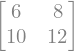
\includegraphics{module_1_files/figure-pdf/cell-3-output-2.png}

\begin{quote}
\emph{Example 2: Matrix Subtraction}
\end{quote}

\emph{Pseudocode:}

\begin{Shaded}
\begin{Highlighting}[]
\CommentTok{\# Define matrices A and B}
\NormalTok{A }\OperatorTok{=}\NormalTok{ [[}\DecValTok{5}\NormalTok{, }\DecValTok{6}\NormalTok{], [}\DecValTok{7}\NormalTok{, }\DecValTok{8}\NormalTok{]]}
\NormalTok{B }\OperatorTok{=}\NormalTok{ [[}\DecValTok{1}\NormalTok{, }\DecValTok{2}\NormalTok{], [}\DecValTok{3}\NormalTok{, }\DecValTok{4}\NormalTok{]]}

\CommentTok{\# Check if matrices A and B have the same dimensions}
\ControlFlowTok{if}\NormalTok{ dimensions\_of(A) }\OperatorTok{!=}\NormalTok{ dimensions\_of(B):}
    \ControlFlowTok{raise} \PreprocessorTok{ValueError}\NormalTok{(}\StringTok{"Matrices must have the same dimensions"}\NormalTok{)}

\CommentTok{\# Initialize result matrix with zeros}
\NormalTok{result }\OperatorTok{=}\NormalTok{ [[}\DecValTok{0} \ControlFlowTok{for}\NormalTok{ \_ }\KeywordTok{in} \BuiltInTok{range}\NormalTok{(}\BuiltInTok{len}\NormalTok{(A[}\DecValTok{0}\NormalTok{]))] }\ControlFlowTok{for}\NormalTok{ \_ }\KeywordTok{in} \BuiltInTok{range}\NormalTok{(}\BuiltInTok{len}\NormalTok{(A))]}

\CommentTok{\# Subtract corresponding elements from A and B}
\ControlFlowTok{for}\NormalTok{ i }\KeywordTok{in} \BuiltInTok{range}\NormalTok{(}\BuiltInTok{len}\NormalTok{(A)):}
    \ControlFlowTok{for}\NormalTok{ j }\KeywordTok{in} \BuiltInTok{range}\NormalTok{(}\BuiltInTok{len}\NormalTok{(A[}\DecValTok{0}\NormalTok{])):}
\NormalTok{        result[i][j] }\OperatorTok{=}\NormalTok{ A[i][j] }\OperatorTok{{-}}\NormalTok{ B[i][j]}

\CommentTok{\# Return the result matrix}
\ControlFlowTok{return}\NormalTok{ result}
\end{Highlighting}
\end{Shaded}

Python implementation of the above pseudocode is given below:

\begin{Shaded}
\begin{Highlighting}[]
\ImportTok{from}\NormalTok{ sympy }\ImportTok{import}\NormalTok{ Matrix}
\CommentTok{\# Define matrices A and B}
\NormalTok{A }\OperatorTok{=}\NormalTok{ Matrix([[}\DecValTok{5}\NormalTok{, }\DecValTok{6}\NormalTok{], [}\DecValTok{7}\NormalTok{, }\DecValTok{8}\NormalTok{]])}
\NormalTok{B }\OperatorTok{=}\NormalTok{ Matrix([[}\DecValTok{1}\NormalTok{, }\DecValTok{2}\NormalTok{], [}\DecValTok{3}\NormalTok{, }\DecValTok{4}\NormalTok{]])}

\CommentTok{\# Subtract matrices}
\NormalTok{C }\OperatorTok{=}\NormalTok{ A }\OperatorTok{{-}}\NormalTok{ B}

\CommentTok{\# Print the result in symbolic form}
\BuiltInTok{print}\NormalTok{(}\StringTok{"Matrix Subtraction Result:"}\NormalTok{)}
\NormalTok{display(C)}

\CommentTok{\# Convert to LaTeX code for documentation or presentation}
\NormalTok{latex\_code }\OperatorTok{=}\NormalTok{ sy.latex(C)}
\BuiltInTok{print}\NormalTok{(}\StringTok{"LaTeX Code for Subtraction Result:"}\NormalTok{)}
\BuiltInTok{print}\NormalTok{(latex\_code)}
\end{Highlighting}
\end{Shaded}

\begin{verbatim}
Matrix Subtraction Result:
\end{verbatim}

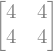
\includegraphics{module_1_files/figure-pdf/cell-4-output-2.png}

\begin{verbatim}
LaTeX Code for Subtraction Result:
\left[\begin{matrix}4 & 4\\4 & 4\end{matrix}\right]
\end{verbatim}

\begin{quote}
\textbf{Example 3: Matrix Multiplication}
\end{quote}

\emph{Pseudocode:}

\begin{Shaded}
\begin{Highlighting}[]
\CommentTok{\# Define matrices A and B}
\NormalTok{A }\OperatorTok{=}\NormalTok{ [[}\DecValTok{1}\NormalTok{, }\DecValTok{2}\NormalTok{], [}\DecValTok{3}\NormalTok{, }\DecValTok{4}\NormalTok{]]}
\NormalTok{B }\OperatorTok{=}\NormalTok{ [[}\DecValTok{5}\NormalTok{, }\DecValTok{6}\NormalTok{], [}\DecValTok{7}\NormalTok{, }\DecValTok{8}\NormalTok{]]}

\CommentTok{\# Check if the number of columns in A equals the number of rows in B}
\ControlFlowTok{if} \BuiltInTok{len}\NormalTok{(A[}\DecValTok{0}\NormalTok{]) }\OperatorTok{!=} \BuiltInTok{len}\NormalTok{(B):}
    \ControlFlowTok{raise} \PreprocessorTok{ValueError}\NormalTok{(}\StringTok{"Number of columns in A must equal number of rows in B"}\NormalTok{)}

\CommentTok{\# Initialize result matrix with zeros}
\NormalTok{result }\OperatorTok{=}\NormalTok{ [[}\DecValTok{0} \ControlFlowTok{for}\NormalTok{ \_ }\KeywordTok{in} \BuiltInTok{range}\NormalTok{(}\BuiltInTok{len}\NormalTok{(B[}\DecValTok{0}\NormalTok{]))] }\ControlFlowTok{for}\NormalTok{ \_ }\KeywordTok{in} \BuiltInTok{range}\NormalTok{(}\BuiltInTok{len}\NormalTok{(A))]}

\CommentTok{\# Multiply matrices A and B}
\ControlFlowTok{for}\NormalTok{ i }\KeywordTok{in} \BuiltInTok{range}\NormalTok{(}\BuiltInTok{len}\NormalTok{(A)):}
    \ControlFlowTok{for}\NormalTok{ j }\KeywordTok{in} \BuiltInTok{range}\NormalTok{(}\BuiltInTok{len}\NormalTok{(B[}\DecValTok{0}\NormalTok{])):}
        \ControlFlowTok{for}\NormalTok{ k }\KeywordTok{in} \BuiltInTok{range}\NormalTok{(}\BuiltInTok{len}\NormalTok{(B)):}
\NormalTok{            result[i][j] }\OperatorTok{+=}\NormalTok{ A[i][k] }\OperatorTok{*}\NormalTok{ B[k][j]}

\CommentTok{\# Return the result matrix}
\ControlFlowTok{return}\NormalTok{ result}
\end{Highlighting}
\end{Shaded}

Python implementation of the above pseudocode is given below:

\begin{Shaded}
\begin{Highlighting}[]
\CommentTok{\# Define matrices A and B}
\NormalTok{A }\OperatorTok{=}\NormalTok{ Matrix([[}\DecValTok{1}\NormalTok{, }\DecValTok{2}\NormalTok{], [}\DecValTok{3}\NormalTok{, }\DecValTok{4}\NormalTok{]])}
\NormalTok{B }\OperatorTok{=}\NormalTok{ Matrix([[}\DecValTok{5}\NormalTok{, }\DecValTok{6}\NormalTok{], [}\DecValTok{7}\NormalTok{, }\DecValTok{8}\NormalTok{]])}

\CommentTok{\# Multiply matrices}
\NormalTok{M }\OperatorTok{=}\NormalTok{ A }\OperatorTok{*}\NormalTok{ B}

\CommentTok{\# Print the result in symbolic form}
\BuiltInTok{print}\NormalTok{(}\StringTok{"Matrix Multiplication Result:"}\NormalTok{)}
\NormalTok{display(M)}

\CommentTok{\# Convert to LaTeX code for documentation or presentation}
\NormalTok{latex\_code }\OperatorTok{=}\NormalTok{ sy.latex(M)}
\BuiltInTok{print}\NormalTok{(}\StringTok{"LaTeX Code for Multiplication Result:"}\NormalTok{)}
\BuiltInTok{print}\NormalTok{(latex\_code)}
\end{Highlighting}
\end{Shaded}

\begin{verbatim}
Matrix Multiplication Result:
\end{verbatim}

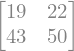
\includegraphics{module_1_files/figure-pdf/cell-5-output-2.png}

\begin{verbatim}
LaTeX Code for Multiplication Result:
\left[\begin{matrix}19 & 22\\43 & 50\end{matrix}\right]
\end{verbatim}

\begin{quote}
\textbf{Example 3: Matrix Multiplication}
\end{quote}

\emph{Pseudocode:}

\begin{Shaded}
\begin{Highlighting}[]
\CommentTok{\# Define matrices A and B}
\NormalTok{A }\OperatorTok{=}\NormalTok{ [[}\DecValTok{1}\NormalTok{, }\DecValTok{2}\NormalTok{], [}\DecValTok{3}\NormalTok{, }\DecValTok{4}\NormalTok{]]}
\NormalTok{B }\OperatorTok{=}\NormalTok{ [[}\DecValTok{5}\NormalTok{, }\DecValTok{6}\NormalTok{], [}\DecValTok{7}\NormalTok{, }\DecValTok{8}\NormalTok{]]}

\CommentTok{\# Check if the number of columns in A equals the number of rows in B}
\ControlFlowTok{if} \BuiltInTok{len}\NormalTok{(A[}\DecValTok{0}\NormalTok{]) }\OperatorTok{!=} \BuiltInTok{len}\NormalTok{(B):}
    \ControlFlowTok{raise} \PreprocessorTok{ValueError}\NormalTok{(}\StringTok{"Number of columns in A must equal number of rows in B"}\NormalTok{)}

\CommentTok{\# Initialize result matrix with zeros}
\NormalTok{result }\OperatorTok{=}\NormalTok{ [[}\DecValTok{0} \ControlFlowTok{for}\NormalTok{ \_ }\KeywordTok{in} \BuiltInTok{range}\NormalTok{(}\BuiltInTok{len}\NormalTok{(B[}\DecValTok{0}\NormalTok{]))] }\ControlFlowTok{for}\NormalTok{ \_ }\KeywordTok{in} \BuiltInTok{range}\NormalTok{(}\BuiltInTok{len}\NormalTok{(A))]}

\CommentTok{\# Multiply matrices A and B}
\ControlFlowTok{for}\NormalTok{ i }\KeywordTok{in} \BuiltInTok{range}\NormalTok{(}\BuiltInTok{len}\NormalTok{(A)):}
    \ControlFlowTok{for}\NormalTok{ j }\KeywordTok{in} \BuiltInTok{range}\NormalTok{(}\BuiltInTok{len}\NormalTok{(B[}\DecValTok{0}\NormalTok{])):}
        \ControlFlowTok{for}\NormalTok{ k }\KeywordTok{in} \BuiltInTok{range}\NormalTok{(}\BuiltInTok{len}\NormalTok{(B)):}
\NormalTok{            result[i][j] }\OperatorTok{+=}\NormalTok{ A[i][k] }\OperatorTok{*}\NormalTok{ B[k][j]}

\CommentTok{\# Return the result matrix}
\ControlFlowTok{return}\NormalTok{ result}
\end{Highlighting}
\end{Shaded}

Python code for implementing the above pseudocode is shown below:

\begin{Shaded}
\begin{Highlighting}[]
\CommentTok{\# Define matrices A and B}
\NormalTok{A }\OperatorTok{=}\NormalTok{ Matrix([[}\DecValTok{1}\NormalTok{, }\DecValTok{2}\NormalTok{], [}\DecValTok{3}\NormalTok{, }\DecValTok{4}\NormalTok{]])}
\NormalTok{B }\OperatorTok{=}\NormalTok{ Matrix([[}\DecValTok{5}\NormalTok{, }\DecValTok{6}\NormalTok{], [}\DecValTok{7}\NormalTok{, }\DecValTok{8}\NormalTok{]])}

\CommentTok{\# Multiply matrices}
\NormalTok{M }\OperatorTok{=}\NormalTok{ A }\OperatorTok{*}\NormalTok{ B}

\CommentTok{\# Print the result in symbolic form}
\BuiltInTok{print}\NormalTok{(}\StringTok{"Matrix Multiplication Result:"}\NormalTok{)}
\NormalTok{display(M)}

\CommentTok{\# Convert to LaTeX code for documentation or presentation}
\NormalTok{latex\_code }\OperatorTok{=}\NormalTok{ sy.latex(M)}
\BuiltInTok{print}\NormalTok{(}\StringTok{"LaTeX Code for Multiplication Result:"}\NormalTok{)}
\BuiltInTok{print}\NormalTok{(latex\_code)}
\end{Highlighting}
\end{Shaded}

\begin{verbatim}
Matrix Multiplication Result:
\end{verbatim}

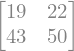
\includegraphics{module_1_files/figure-pdf/cell-6-output-2.png}

\begin{verbatim}
LaTeX Code for Multiplication Result:
\left[\begin{matrix}19 & 22\\43 & 50\end{matrix}\right]
\end{verbatim}

\begin{quote}
\textbf{Example 4: Matrix Power}
\end{quote}

\emph{Pseudocode:}

\begin{Shaded}
\begin{Highlighting}[]
\CommentTok{\# Define matrix A and power n}
\NormalTok{A }\OperatorTok{=}\NormalTok{ [[}\DecValTok{1}\NormalTok{, }\DecValTok{2}\NormalTok{], [}\DecValTok{3}\NormalTok{, }\DecValTok{4}\NormalTok{]]}
\NormalTok{n }\OperatorTok{=} \DecValTok{2}

\CommentTok{\# Initialize result matrix as identity matrix}
\NormalTok{result }\OperatorTok{=}\NormalTok{ identity\_matrix\_of(}\BuiltInTok{len}\NormalTok{(A))}

\CommentTok{\# Compute A raised to the power of n}
\ControlFlowTok{for}\NormalTok{ \_ }\KeywordTok{in} \BuiltInTok{range}\NormalTok{(n):}
\NormalTok{    result }\OperatorTok{=}\NormalTok{ matrix\_multiply(result, A)}

\CommentTok{\# Return the result matrix}
\ControlFlowTok{return}\NormalTok{ result}
\end{Highlighting}
\end{Shaded}

Python implementation of the above pseudocode is shown below:

\begin{Shaded}
\begin{Highlighting}[]
\CommentTok{\# Define matrix A}
\NormalTok{A }\OperatorTok{=}\NormalTok{ Matrix([[}\DecValTok{1}\NormalTok{, }\DecValTok{2}\NormalTok{], [}\DecValTok{3}\NormalTok{, }\DecValTok{4}\NormalTok{]])}

\CommentTok{\# Compute matrix A raised to the power of 2}
\NormalTok{n }\OperatorTok{=} \DecValTok{2}
\NormalTok{C }\OperatorTok{=}\NormalTok{ A}\OperatorTok{**}\NormalTok{n}

\CommentTok{\# Print the result in symbolic form}
\BuiltInTok{print}\NormalTok{(}\StringTok{"Matrix Power Result:"}\NormalTok{)}
\NormalTok{display(C)}

\CommentTok{\# Convert to LaTeX code for documentation or presentation}
\NormalTok{latex\_code }\OperatorTok{=}\NormalTok{ sy.latex(C)}
\BuiltInTok{print}\NormalTok{(}\StringTok{"LaTeX Code for Power Result:"}\NormalTok{)}
\BuiltInTok{print}\NormalTok{(latex\_code)}
\end{Highlighting}
\end{Shaded}

\begin{verbatim}
Matrix Power Result:
\end{verbatim}

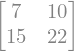
\includegraphics{module_1_files/figure-pdf/cell-7-output-2.png}

\begin{verbatim}
LaTeX Code for Power Result:
\left[\begin{matrix}7 & 10\\15 & 22\end{matrix}\right]
\end{verbatim}

\subsubsection{Introduction to PIL for Image
Manipulation}\label{introduction-to-pil-for-image-manipulation}

The \texttt{PIL} (Python Imaging Library), now known as \texttt{Pillow},
provides essential tools for opening, manipulating, and saving various
image file formats. In this session, we will use Pillow to perform image
operations such as resizing and blending to demonstrate the practical
applications of these matrix operations in digital image processing.

Matrix operations have significant applications in digital image
processing. These operations can manipulate images in various ways, from
blending to filtering. Below we will discuss how matrix addition,
subtraction, and multiplication are used in real-time image processing
tasks.

\begin{enumerate}
\def\labelenumi{\arabic{enumi}.}
\tightlist
\item
  \textbf{Matrix Addition: Image Blending}
\end{enumerate}

Matrix addition can be used to blend two images by adding their pixel
values. This process can be straightforward or involve weighted
blending.

Example 1: Simple Image Blending

\begin{Shaded}
\begin{Highlighting}[]
\ImportTok{import}\NormalTok{ numpy }\ImportTok{as}\NormalTok{ np}
\ImportTok{from}\NormalTok{ PIL }\ImportTok{import}\NormalTok{ Image}
\ImportTok{import}\NormalTok{ urllib.request}
\NormalTok{urllib.request.urlretrieve(}\StringTok{\textquotesingle{}http://lenna.org/len\_top.jpg\textquotesingle{}}\NormalTok{,}\StringTok{"input.jpg"}\NormalTok{)}
\NormalTok{img1 }\OperatorTok{=}\NormalTok{ Image.}\BuiltInTok{open}\NormalTok{(}\StringTok{"input.jpg"}\NormalTok{) }\CommentTok{\#loading first image}

\NormalTok{urllib.request.urlretrieve(}\StringTok{\textquotesingle{}https://www.keralatourism.org/images/destination/large/thekkekudi\_cave\_temple\_in\_pathanamthitta20131205062431\_315\_1.jpg\textquotesingle{}}\NormalTok{,}\StringTok{"input2.jpg"}\NormalTok{)}

\NormalTok{img2 }\OperatorTok{=}\NormalTok{ Image.}\BuiltInTok{open}\NormalTok{(}\StringTok{"input2.jpg"}\NormalTok{)}\CommentTok{\# loading second image}

\CommentTok{\# Resize second image to match the size of the first image}
\NormalTok{img2 }\OperatorTok{=}\NormalTok{ img2.resize(img1.size)}
\CommentTok{\# Convert images to numpy arrays}
\NormalTok{arr1 }\OperatorTok{=}\NormalTok{ np.array(img1)}
\NormalTok{arr2 }\OperatorTok{=}\NormalTok{ np.array(img2)}

\CommentTok{\# Add the images}
\NormalTok{blended\_arr }\OperatorTok{=}\NormalTok{ arr1 }\OperatorTok{+}\NormalTok{ arr2}

\CommentTok{\# Clip the values to be in the valid range [0, 255]}
\NormalTok{blended\_arr }\OperatorTok{=}\NormalTok{ np.clip(blended\_arr, }\DecValTok{0}\NormalTok{, }\DecValTok{255}\NormalTok{).astype(np.uint8)}

\CommentTok{\# Convert back to image}
\NormalTok{blended\_img }\OperatorTok{=}\NormalTok{ Image.fromarray(blended\_arr)}

\CommentTok{\# Save or display the blended image}
\CommentTok{\#blended\_img.save(\textquotesingle{}blended\_image.jpg\textquotesingle{})}
\CommentTok{\#blended\_img.show()}
\CommentTok{\#blended\_img \#display the blended image}
\end{Highlighting}
\end{Shaded}

The input and output images are shown below:

\begin{Shaded}
\begin{Highlighting}[]
\NormalTok{img1}
\end{Highlighting}
\end{Shaded}

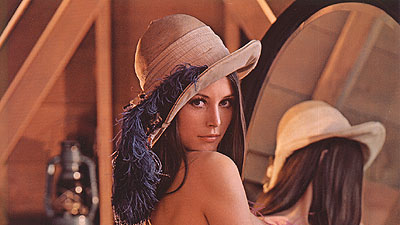
\includegraphics{module_1_files/figure-pdf/cell-9-output-1.png}

\begin{Shaded}
\begin{Highlighting}[]
\NormalTok{img2}
\end{Highlighting}
\end{Shaded}

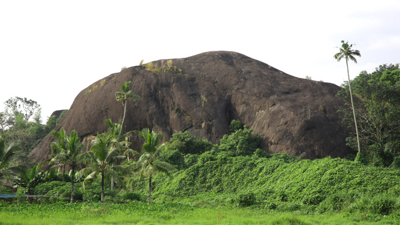
\includegraphics{module_1_files/figure-pdf/cell-10-output-1.png}

\begin{Shaded}
\begin{Highlighting}[]
\NormalTok{blended\_img}
\end{Highlighting}
\end{Shaded}

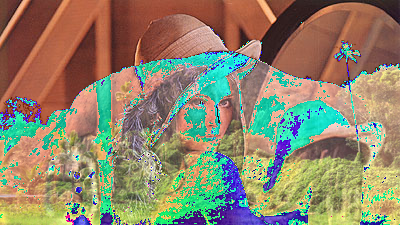
\includegraphics{module_1_files/figure-pdf/cell-11-output-1.png}

\begin{quote}
\textbf{Example 2: Weighted Image Blending}
\end{quote}

\begin{Shaded}
\begin{Highlighting}[]
\CommentTok{\# Blend with weights}
\NormalTok{alpha }\OperatorTok{=} \FloatTok{0.7}
\NormalTok{blended\_arr }\OperatorTok{=}\NormalTok{ alpha }\OperatorTok{*}\NormalTok{ arr1 }\OperatorTok{+}\NormalTok{ (}\DecValTok{1} \OperatorTok{{-}}\NormalTok{ alpha) }\OperatorTok{*}\NormalTok{ arr2}

\CommentTok{\# Clip the values to be in the valid range [0, 255]}
\NormalTok{blended\_arr }\OperatorTok{=}\NormalTok{ np.clip(blended\_arr, }\DecValTok{0}\NormalTok{, }\DecValTok{255}\NormalTok{).astype(np.uint8)}

\CommentTok{\# Convert back to image}
\NormalTok{blended\_img }\OperatorTok{=}\NormalTok{ Image.fromarray(blended\_arr)}

\CommentTok{\# Save or display the weighted blended image}
\CommentTok{\#blended\_img.save(\textquotesingle{}weighted\_blended\_image.jpg\textquotesingle{})}
\CommentTok{\#blended\_img.show()}
\NormalTok{blended\_img}
\end{Highlighting}
\end{Shaded}

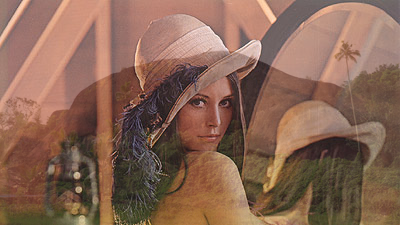
\includegraphics{module_1_files/figure-pdf/cell-12-output-1.png}

\subsubsection{Matrix Subtraction: Image
Sharpening}\label{matrix-subtraction-image-sharpening}

Matrix subtraction can be used to sharpen images by subtracting a
blurred version of the image from the original.

\begin{quote}
\textbf{Example 1: Sharpening by Subtracting Blurred Image}
\end{quote}

\begin{Shaded}
\begin{Highlighting}[]
\ImportTok{from}\NormalTok{ PIL }\ImportTok{import}\NormalTok{ Image, ImageFilter}
\CommentTok{\# Convert image to grayscale for simplicity}
\NormalTok{img\_gray }\OperatorTok{=}\NormalTok{ img1.convert(}\StringTok{\textquotesingle{}L\textquotesingle{}}\NormalTok{)}
\NormalTok{arr }\OperatorTok{=}\NormalTok{ np.array(img\_gray)}

\CommentTok{\# Apply Gaussian blur}
\NormalTok{blurred\_img }\OperatorTok{=}\NormalTok{ img\_gray.}\BuiltInTok{filter}\NormalTok{(ImageFilter.GaussianBlur(radius}\OperatorTok{=}\DecValTok{5}\NormalTok{))}
\NormalTok{blurred\_arr }\OperatorTok{=}\NormalTok{ np.array(blurred\_img)}

\CommentTok{\# Sharpen the image by subtracting blurred image}
\NormalTok{sharpened\_arr }\OperatorTok{=}\NormalTok{ arr }\OperatorTok{{-}}\NormalTok{ blurred\_arr}

\CommentTok{\# Clip the values to be in the valid range [0, 255]}
\NormalTok{sharpened\_arr }\OperatorTok{=}\NormalTok{ np.clip(sharpened\_arr, }\DecValTok{0}\NormalTok{, }\DecValTok{255}\NormalTok{).astype(np.uint8)}

\CommentTok{\# Convert back to image}
\NormalTok{sharpened\_img }\OperatorTok{=}\NormalTok{ Image.fromarray(sharpened\_arr)}

\CommentTok{\# Save or display the sharpened image}
\CommentTok{\#sharpened\_img.save(\textquotesingle{}sharpened\_image.jpg\textquotesingle{})}
\CommentTok{\#sharpened\_img.show()}
\NormalTok{sharpened\_img}
\end{Highlighting}
\end{Shaded}


\includegraphics{module_1_files/figure-pdf/cell-13-output-1.png}

\subsubsection{Matrix Multiplication: Image Filtering
(Convolution)}\label{matrix-multiplication-image-filtering-convolution}

Matrix multiplication is used in image filtering to apply convolution
kernels for various effects.

\begin{quote}
\textbf{Example 1: Applying a Convolution Filter}
\end{quote}

\begin{Shaded}
\begin{Highlighting}[]
\CommentTok{\# Define a simple convolution kernel (e.g., edge detection)}
\NormalTok{kernel }\OperatorTok{=}\NormalTok{ np.array([}
\NormalTok{    [}\DecValTok{1}\NormalTok{, }\DecValTok{0}\NormalTok{, }\OperatorTok{{-}}\DecValTok{1}\NormalTok{],}
\NormalTok{    [}\DecValTok{1}\NormalTok{, }\DecValTok{0}\NormalTok{, }\OperatorTok{{-}}\DecValTok{1}\NormalTok{],}
\NormalTok{    [}\DecValTok{1}\NormalTok{, }\DecValTok{0}\NormalTok{, }\OperatorTok{{-}}\DecValTok{1}\NormalTok{]}
\NormalTok{])}

\CommentTok{\# Convert the image to grayscale for simplicity}
\NormalTok{img\_gray }\OperatorTok{=}\NormalTok{ img1.convert(}\StringTok{\textquotesingle{}L\textquotesingle{}}\NormalTok{)}
\NormalTok{arr }\OperatorTok{=}\NormalTok{ np.array(img\_gray)}

\CommentTok{\# Apply convolution}
\NormalTok{filtered\_arr }\OperatorTok{=}\NormalTok{ np.zeros\_like(arr)}
\ControlFlowTok{for}\NormalTok{ i }\KeywordTok{in} \BuiltInTok{range}\NormalTok{(}\DecValTok{1}\NormalTok{, arr.shape[}\DecValTok{0}\NormalTok{] }\OperatorTok{{-}} \DecValTok{1}\NormalTok{):}
    \ControlFlowTok{for}\NormalTok{ j }\KeywordTok{in} \BuiltInTok{range}\NormalTok{(}\DecValTok{1}\NormalTok{, arr.shape[}\DecValTok{1}\NormalTok{] }\OperatorTok{{-}} \DecValTok{1}\NormalTok{):}
\NormalTok{        region }\OperatorTok{=}\NormalTok{ arr[i}\OperatorTok{{-}}\DecValTok{1}\NormalTok{:i}\OperatorTok{+}\DecValTok{2}\NormalTok{, j}\OperatorTok{{-}}\DecValTok{1}\NormalTok{:j}\OperatorTok{+}\DecValTok{2}\NormalTok{]}
\NormalTok{        filtered\_arr[i, j] }\OperatorTok{=}\NormalTok{ np.}\BuiltInTok{sum}\NormalTok{(region }\OperatorTok{*}\NormalTok{ kernel)}

\CommentTok{\# Convert back to image}
\NormalTok{filtered\_img }\OperatorTok{=}\NormalTok{ Image.fromarray(np.clip(filtered\_arr, }\DecValTok{0}\NormalTok{, }\DecValTok{255}\NormalTok{).astype(np.uint8))}

\CommentTok{\# Save or display the filtered image}
\CommentTok{\#filtered\_img.save(\textquotesingle{}filtered\_image.jpg\textquotesingle{})}
\CommentTok{\#filtered\_img.show()}
\NormalTok{filtered\_img}
\end{Highlighting}
\end{Shaded}

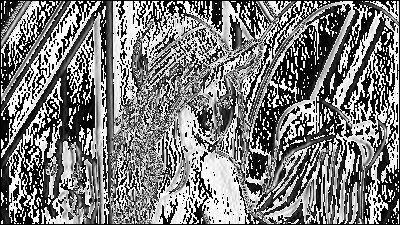
\includegraphics{module_1_files/figure-pdf/cell-14-output-1.png}

\begin{quote}
\textbf{Example 2: Applying a Gaussian Blur Filter}
\end{quote}

\begin{Shaded}
\begin{Highlighting}[]
\CommentTok{\# Define a Gaussian blur filter}
\NormalTok{blurred\_img }\OperatorTok{=}\NormalTok{ img1.}\BuiltInTok{filter}\NormalTok{(ImageFilter.GaussianBlur(radius}\OperatorTok{=}\DecValTok{5}\NormalTok{))}

\CommentTok{\# Save or display the blurred image}
\CommentTok{\#blurred\_img.save(\textquotesingle{}blurred\_image.jpg\textquotesingle{})}
\CommentTok{\#blurred\_img.show()}
\NormalTok{blurred\_img}
\end{Highlighting}
\end{Shaded}


\includegraphics{module_1_files/figure-pdf/cell-15-output-1.png}

\subsubsection{Solving Systems of Equations and
Applications}\label{solving-systems-of-equations-and-applications}

\textbf{Introduction}

Solving systems of linear equations is crucial in various image
processing tasks, such as image transformation, camera calibration, and
object detection. In this section, we will demonstrate how to solve
systems of linear equations using Python and explore practical
applications in image processing.

\begin{quote}
\textbf{Example 1: Solving a System of Equations}
\end{quote}

Consider the system:

\[\begin{cases}
2x + 3y& = 13 \\
4x - y &= 7
\end{cases}\]

\begin{quote}
\textbf{Python Implementation}
\end{quote}

\begin{Shaded}
\begin{Highlighting}[]
\ImportTok{from}\NormalTok{ sympy }\ImportTok{import}\NormalTok{ Matrix}
\CommentTok{\# Define the coefficient matrix and constant matrix}
\NormalTok{A }\OperatorTok{=}\NormalTok{ Matrix([[}\DecValTok{2}\NormalTok{, }\DecValTok{3}\NormalTok{], [}\DecValTok{4}\NormalTok{, }\OperatorTok{{-}}\DecValTok{1}\NormalTok{]])}
\NormalTok{B }\OperatorTok{=}\NormalTok{ Matrix([}\DecValTok{13}\NormalTok{, }\DecValTok{7}\NormalTok{])}
\CommentTok{\# Solve the system of equations}
\NormalTok{solution }\OperatorTok{=}\NormalTok{ A.solve\_least\_squares(B)}
\CommentTok{\# Print the solution}
\BuiltInTok{print}\NormalTok{(}\StringTok{"Solution to the System of Equations:"}\NormalTok{)}
\BuiltInTok{print}\NormalTok{(solution)}
\end{Highlighting}
\end{Shaded}

\begin{verbatim}
Solution to the System of Equations:
Matrix([[17/7], [19/7]])
\end{verbatim}

\section{Conclusion}\label{conclusion}

In this chapter, we transitioned from understanding fundamental matrix
operations to applying them in practical scenarios, specifically in the
realm of image processing. We began by covering essential matrix
operations such as addition, subtraction, multiplication, and
determinant calculations, providing both pseudocode and detailed
explanations. This foundational knowledge was then translated into
Python code, demonstrating how to perform these operations
computationally.

We further explored the application of these matrix operations to
real-world image processing tasks. By applying techniques such as image
blending, sharpening, filtering, and transformation, we illustrated how
theoretical concepts can be used to manipulate and enhance digital
images effectively. These practical examples highlighted the
significance of matrix operations in solving complex image processing
challenges.

By integrating theoretical understanding with practical implementation,
this chapter reinforced how matrix operations form the backbone of many
image processing techniques. This blend of theory and practice equips
you with essential skills for tackling advanced problems and developing
innovative solutions in the field of image processing and beyond.

\bookmarksetup{startatroot}

\chapter{Transforming Linear Algebra to Computational
Language}\label{transforming-linear-algebra-to-computational-language}

\section{Introduction}\label{introduction-2}

In the first module, we established a solid foundation in matrix algebra
by exploring pseudocode and implementing fundamental matrix operations
using \texttt{Python}. We practiced key concepts such as matrix
addition, subtraction, multiplication, and determinants through
practical examples in image processing, leveraging the \texttt{SymPy}
library for symbolic computation.

As we begin the second module, \textbf{``Transforming Linear Algebra to
Computational Language,''} our focus will shift towards applying these
concepts with greater depth and actionable insight. This module is
designed to bridge the theoretical knowledge from matrix algebra with
practical computational applications. You will learn to interpret and
utilize matrix operations, solve systems of equations, and analyze the
rank of matrices within a variety of real-world contexts.

A new concept we will introduce is the \textbf{Rank-Nullity Theorem},
which provides a fundamental relationship between the rank of a matrix
and the dimensions of its null space. This theorem is crucial for
understanding the solution spaces of linear systems and the properties
of linear transformations. By applying this theorem, you will be able to
gain deeper insights into the structure of solutions and the behavior of
matrix transformations.

This transition will not only reinforce your understanding of linear
algebra but also enhance your ability to apply these concepts
effectively in computational settings. Through engaging examples and
practical exercises, you will gain valuable experience in transforming
abstract mathematical principles into tangible solutions, setting a
strong groundwork for advanced computational techniques.

\section{Relearning of Terms and Operations in Linear
Algebra}\label{relearning-of-terms-and-operations-in-linear-algebra}

In this section, we will revisit fundamental matrix operations such as
addition, subtraction, scaling, and more through practical examples. Our
goal is to transform theoretical linear algebra into modern
computational applications. We will demonstrate these concepts using
\texttt{Python}, focusing on practical and industrial applications.

\subsection{Matrix Addition and Subtraction in Data
Analysis}\label{matrix-addition-and-subtraction-in-data-analysis}

Matrix addition and subtraction are fundamental operations that help in
combining datasets and analyzing differences.

\textbf{Simple Example: Combining Quarterly Sales Data}

We begin with quarterly sales data from different regions and combine
them to get the total sales. The sales data is given in
Table~\ref{tbl-qtb}. A ar plot of the total sales is shown in
Fig~\ref{fig-total1}.

\begin{longtable}[]{@{}lllll@{}}
\caption{Quarterly Sales Data}\label{tbl-qtb}\tabularnewline
\toprule\noalign{}
Region & Q1 & Q2 & Q3 & Q4 \\
\midrule\noalign{}
\endfirsthead
\toprule\noalign{}
Region & Q1 & Q2 & Q3 & Q4 \\
\midrule\noalign{}
\endhead
\bottomrule\noalign{}
\endlastfoot
A & 2500 & 2800 & 3100 & 2900 \\
B & 1500 & 1600 & 1700 & 1800 \\
\end{longtable}

\textbf{From Scratch \texttt{Python} Implementation:}

\begin{Shaded}
\begin{Highlighting}[]
\ImportTok{import}\NormalTok{ numpy }\ImportTok{as}\NormalTok{ np}
\ImportTok{import}\NormalTok{ matplotlib.pyplot }\ImportTok{as}\NormalTok{ plt}

\CommentTok{\# Quarterly sales data}
\NormalTok{sales\_region\_a }\OperatorTok{=}\NormalTok{ np.array([}\DecValTok{2500}\NormalTok{, }\DecValTok{2800}\NormalTok{, }\DecValTok{3100}\NormalTok{, }\DecValTok{2900}\NormalTok{])}
\NormalTok{sales\_region\_b }\OperatorTok{=}\NormalTok{ np.array([}\DecValTok{1500}\NormalTok{, }\DecValTok{1600}\NormalTok{, }\DecValTok{1700}\NormalTok{, }\DecValTok{1800}\NormalTok{])}

\CommentTok{\# Combine sales data}
\NormalTok{total\_sales }\OperatorTok{=}\NormalTok{ sales\_region\_a }\OperatorTok{+}\NormalTok{ sales\_region\_b}

\CommentTok{\# Visualization}
\NormalTok{quarters }\OperatorTok{=}\NormalTok{ [}\StringTok{\textquotesingle{}Q1\textquotesingle{}}\NormalTok{, }\StringTok{\textquotesingle{}Q2\textquotesingle{}}\NormalTok{, }\StringTok{\textquotesingle{}Q3\textquotesingle{}}\NormalTok{, }\StringTok{\textquotesingle{}Q4\textquotesingle{}}\NormalTok{]}
\NormalTok{plt.bar(quarters, total\_sales, color}\OperatorTok{=}\StringTok{\textquotesingle{}skyblue\textquotesingle{}}\NormalTok{)}
\NormalTok{plt.xlabel(}\StringTok{\textquotesingle{}Quarter\textquotesingle{}}\NormalTok{)}
\NormalTok{plt.ylabel(}\StringTok{\textquotesingle{}Total Sales\textquotesingle{}}\NormalTok{)}
\NormalTok{plt.title(}\StringTok{\textquotesingle{}Combined Quarterly Sales Data for Regions A and B\textquotesingle{}}\NormalTok{)}
\NormalTok{plt.show()}
\end{Highlighting}
\end{Shaded}

\begin{figure}[H]

\centering{

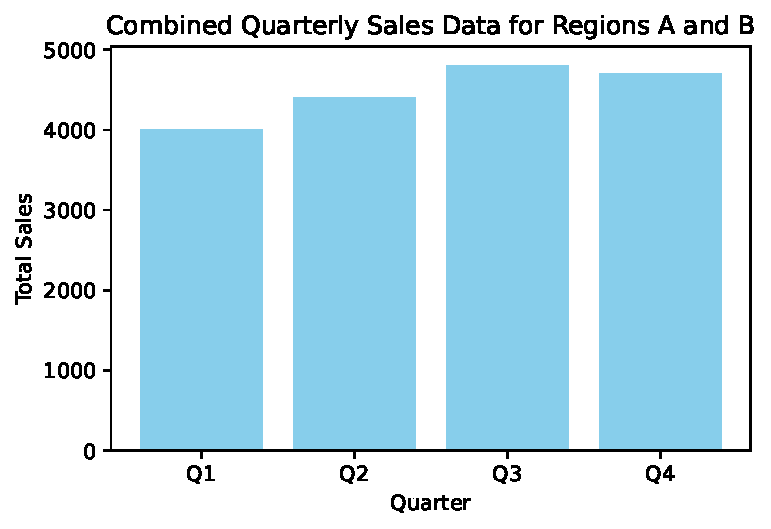
\includegraphics{module_2_files/figure-pdf/fig-total1-output-1.pdf}

}

\caption{\label{fig-total1}Computing Total Sales using \texttt{Numpy}
aggregation method}

\end{figure}%

In the above \texttt{Python} code, we have performed the aggregation
operation with the \texttt{NumPy} method. Same can be done in a more
data analysis style using \texttt{pandas} inorder to handle tabular data
meaningfully. In this approach, quarterly sales data of each region is
stored as \texttt{DataFrames}(like an excel sheet). The we combine these
two \texttt{DataFrames} into one. After that create a new row with index
`Total' and populate this row with sum of quarterly sales in Region A
and Region B. Finally a bar plot is created using this `Total' sales.
Advantage of this approach is that we don't need the \texttt{matplotlib}
library to create visualizations!. The EDA using this approach is shown
in Fig~\ref{fig-tot2}.

\begin{Shaded}
\begin{Highlighting}[]
\ImportTok{import}\NormalTok{ pandas }\ImportTok{as}\NormalTok{ pd}
\ImportTok{import}\NormalTok{ matplotlib.pyplot }\ImportTok{as}\NormalTok{ plt}

\CommentTok{\# DataFrames for quarterly sales data}
\NormalTok{df\_a }\OperatorTok{=}\NormalTok{ pd.DataFrame(\{}\StringTok{\textquotesingle{}Q1\textquotesingle{}}\NormalTok{: [}\DecValTok{2500}\NormalTok{], }\StringTok{\textquotesingle{}Q2\textquotesingle{}}\NormalTok{: [}\DecValTok{2800}\NormalTok{], }\StringTok{\textquotesingle{}Q3\textquotesingle{}}\NormalTok{: [}\DecValTok{3100}\NormalTok{], }\StringTok{\textquotesingle{}Q4\textquotesingle{}}\NormalTok{: [}\DecValTok{2900}\NormalTok{]\}, index}\OperatorTok{=}\NormalTok{[}\StringTok{\textquotesingle{}Region A\textquotesingle{}}\NormalTok{])}
\NormalTok{df\_b }\OperatorTok{=}\NormalTok{ pd.DataFrame(\{}\StringTok{\textquotesingle{}Q1\textquotesingle{}}\NormalTok{: [}\DecValTok{1500}\NormalTok{], }\StringTok{\textquotesingle{}Q2\textquotesingle{}}\NormalTok{: [}\DecValTok{1600}\NormalTok{], }\StringTok{\textquotesingle{}Q3\textquotesingle{}}\NormalTok{: [}\DecValTok{1700}\NormalTok{], }\StringTok{\textquotesingle{}Q4\textquotesingle{}}\NormalTok{: [}\DecValTok{1800}\NormalTok{]\}, index}\OperatorTok{=}\NormalTok{[}\StringTok{\textquotesingle{}Region B\textquotesingle{}}\NormalTok{])}

\CommentTok{\# Combine data}
\NormalTok{df\_combined }\OperatorTok{=}\NormalTok{ df\_a.add(df\_b, fill\_value}\OperatorTok{=}\DecValTok{0}\NormalTok{)}
\NormalTok{df\_combined.loc[}\StringTok{"Total"}\NormalTok{] }\OperatorTok{=}\NormalTok{ df\_combined.}\BuiltInTok{sum}\NormalTok{(axis}\OperatorTok{=}\DecValTok{0}\NormalTok{)}
\CommentTok{\# Visualization}
\NormalTok{df\_combined.loc[}\StringTok{"Total"}\NormalTok{].plot(kind}\OperatorTok{=}\StringTok{\textquotesingle{}bar\textquotesingle{}}\NormalTok{, color}\OperatorTok{=}\NormalTok{[}\StringTok{\textquotesingle{}green\textquotesingle{}}\NormalTok{])}
\NormalTok{plt.xlabel(}\StringTok{\textquotesingle{}Quarter\textquotesingle{}}\NormalTok{)}
\NormalTok{plt.ylabel(}\StringTok{\textquotesingle{}Total Sales\textquotesingle{}}\NormalTok{)}
\NormalTok{plt.title(}\StringTok{\textquotesingle{}Combined Quarterly Sales Data for Regions A and B\textquotesingle{}}\NormalTok{)}
\NormalTok{plt.show()}
\end{Highlighting}
\end{Shaded}

\begin{figure}[H]

\centering{

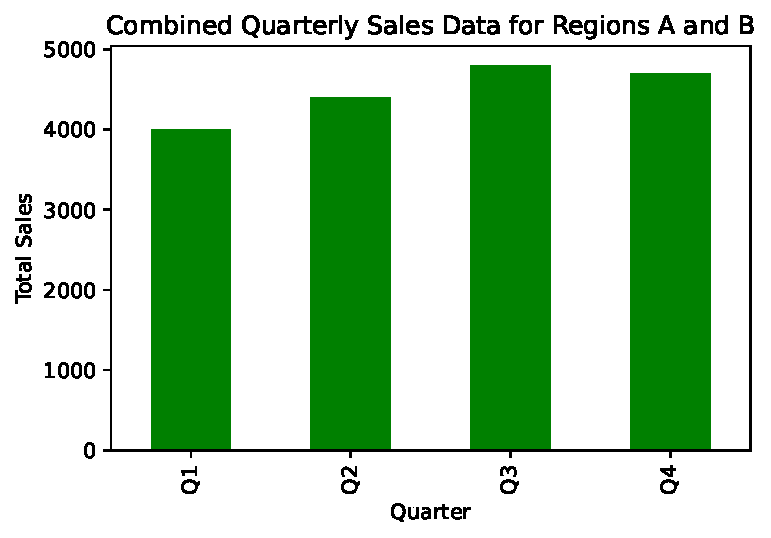
\includegraphics{module_2_files/figure-pdf/fig-tot2-output-1.pdf}

}

\caption{\label{fig-tot2}Computation of Total Sales using
\texttt{Pandas} method}

\end{figure}%

We can extend this in to more advanced examples. Irrespective to the
size of the data, for representation and aggregation tasks matrix models
are best options and are used in industry as a standard. Let us consider
an advanced example to analyse difference in stock prices. For this
example we are using a simulated data. The python code for this
simulation process is shown in Fig~\ref{fig-sim}.

\begin{Shaded}
\begin{Highlighting}[]
\ImportTok{import}\NormalTok{ numpy }\ImportTok{as}\NormalTok{ np}
\ImportTok{import}\NormalTok{ matplotlib.pyplot }\ImportTok{as}\NormalTok{ plt}

\CommentTok{\# Simulated observed and predicted stock prices}
\NormalTok{observed\_prices }\OperatorTok{=}\NormalTok{ np.random.uniform(}\DecValTok{100}\NormalTok{, }\DecValTok{200}\NormalTok{, size}\OperatorTok{=}\NormalTok{(}\DecValTok{100}\NormalTok{, }\DecValTok{5}\NormalTok{))}
\NormalTok{predicted\_prices }\OperatorTok{=}\NormalTok{ np.random.uniform(}\DecValTok{95}\NormalTok{, }\DecValTok{210}\NormalTok{, size}\OperatorTok{=}\NormalTok{(}\DecValTok{100}\NormalTok{, }\DecValTok{5}\NormalTok{))}

\CommentTok{\# Calculate the difference matrix}
\NormalTok{price\_differences }\OperatorTok{=}\NormalTok{ observed\_prices }\OperatorTok{{-}}\NormalTok{ predicted\_prices}

\CommentTok{\# Visualization}
\NormalTok{plt.imshow(price\_differences, cmap}\OperatorTok{=}\StringTok{\textquotesingle{}coolwarm\textquotesingle{}}\NormalTok{, aspect}\OperatorTok{=}\StringTok{\textquotesingle{}auto\textquotesingle{}}\NormalTok{)}
\NormalTok{plt.colorbar()}
\NormalTok{plt.title(}\StringTok{\textquotesingle{}Stock Price Differences\textquotesingle{}}\NormalTok{)}
\NormalTok{plt.xlabel(}\StringTok{\textquotesingle{}Stock Index\textquotesingle{}}\NormalTok{)}
\NormalTok{plt.ylabel(}\StringTok{\textquotesingle{}Day Index\textquotesingle{}}\NormalTok{)}
\NormalTok{plt.show()}
\end{Highlighting}
\end{Shaded}

\begin{figure}[H]

\centering{

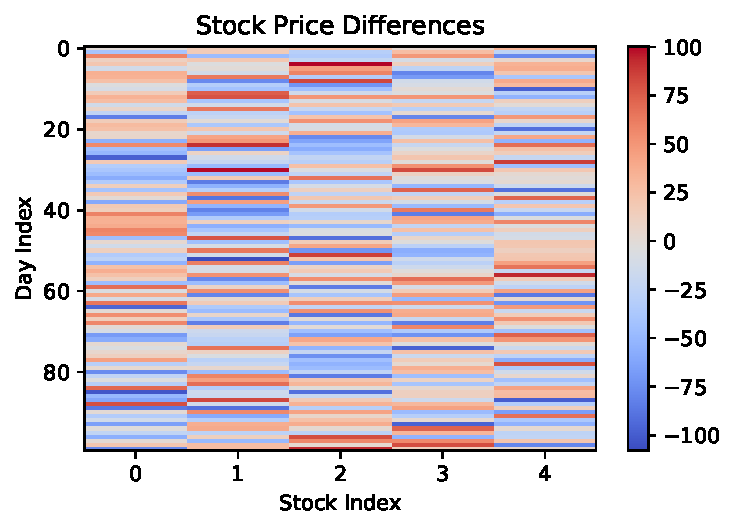
\includegraphics{module_2_files/figure-pdf/fig-sim-output-1.pdf}

}

\caption{\label{fig-sim}Demonstration of Stock Price simulated from a
Uniform Distribution}

\end{figure}%

Another important matrix operation relevant to data analytics and
Machine Learning application is scaling. This is considered as a
statistical tool to make various features (attributes) in to same scale
so as to avoid unnecessary misleading impact in data analysis and its
intepretation. In Machine Learning context, this pre-processing stage is
inevitable so as to make the model relevant and usable.

\textbf{Simple Example: Normalizing Employee Performance Data}

\begin{longtable}[]{@{}lll@{}}
\caption{Employee Performance Data}\label{tbl-EPD}\tabularnewline
\toprule\noalign{}
Employee & Metric A & Metric B \\
\midrule\noalign{}
\endfirsthead
\toprule\noalign{}
Employee & Metric A & Metric B \\
\midrule\noalign{}
\endhead
\bottomrule\noalign{}
\endlastfoot
X & 80 & 700 \\
Y & 90 & 800 \\
Z & 100 & 900 \\
A & 110 & 1000 \\
B & 120 & 1100 \\
\end{longtable}

Using simple python code we can simulate the model for \texttt{min-max}
scaling. The formula for \texttt{min-max} scaling is:
\[min_max(X)=\dfrac{X-min(X)}{max(X)-min(X)}\]

For example, while applying the \texttt{min-max} scaling in the first
value of Metric A, the scaled value is
\[min_max(80)\dfrac{80-80}{120-80}=0\]

Similarly

\[min_max(100)\dfrac{100-80}{120-80}=0.5\]

When we apply this formula to Metric A and Metric B, the scaled output
from Table~\ref{tbl-EPD} will be as follows:

\begin{longtable}[]{@{}lll@{}}
\caption{Employee Performance Data}\label{tbl-EPDu}\tabularnewline
\toprule\noalign{}
Employee & Metric A & Metric B \\
\midrule\noalign{}
\endfirsthead
\toprule\noalign{}
Employee & Metric A & Metric B \\
\midrule\noalign{}
\endhead
\bottomrule\noalign{}
\endlastfoot
X & 0.00 & 0.00 \\
Y & 0.25 & 0.25 \\
Z & 0.50 & 0.50 \\
A & 0.75 & 0.75 \\
B & 1.00 & 1.00 \\
\end{longtable}

It is interesting to look into the scaled data! In the orginal table
(Table~\ref{tbl-EPD}) it is looked like Metric B is superior. But from
the scaled table (Table~\ref{tbl-EPDu}), it is clear that both the
Metrics are representing same relative information. This will help us to
identify the redundency in measure and so skip any one of the Metric
before analysis!.

The same can be achieved through a matrix operation. The \texttt{Python}
implementation of this scaling process is shown in
Fig~\ref{fig-totalsales}.

\begin{Shaded}
\begin{Highlighting}[]
\ImportTok{import}\NormalTok{ numpy }\ImportTok{as}\NormalTok{ np}
\ImportTok{import}\NormalTok{ matplotlib.pyplot }\ImportTok{as}\NormalTok{ plt}

\CommentTok{\# Employee performance data with varying scales}
\NormalTok{data }\OperatorTok{=}\NormalTok{ np.array([[}\DecValTok{80}\NormalTok{, }\DecValTok{700}\NormalTok{], [}\DecValTok{90}\NormalTok{, }\DecValTok{800}\NormalTok{], [}\DecValTok{100}\NormalTok{, }\DecValTok{900}\NormalTok{], [}\DecValTok{110}\NormalTok{, }\DecValTok{1000}\NormalTok{], [}\DecValTok{120}\NormalTok{, }\DecValTok{1100}\NormalTok{]])}

\CommentTok{\# Manual scaling}
\NormalTok{min\_vals }\OperatorTok{=}\NormalTok{ np.}\BuiltInTok{min}\NormalTok{(data, axis}\OperatorTok{=}\DecValTok{0}\NormalTok{)}
\NormalTok{max\_vals }\OperatorTok{=}\NormalTok{ np.}\BuiltInTok{max}\NormalTok{(data, axis}\OperatorTok{=}\DecValTok{0}\NormalTok{)}
\NormalTok{scaled\_data }\OperatorTok{=}\NormalTok{ (data }\OperatorTok{{-}}\NormalTok{ min\_vals) }\OperatorTok{/}\NormalTok{ (max\_vals }\OperatorTok{{-}}\NormalTok{ min\_vals)}

\CommentTok{\# Visualization}
\NormalTok{plt.figure(figsize}\OperatorTok{=}\NormalTok{(}\DecValTok{8}\NormalTok{, }\DecValTok{5}\NormalTok{))}
\NormalTok{plt.subplot(}\DecValTok{1}\NormalTok{, }\DecValTok{2}\NormalTok{, }\DecValTok{1}\NormalTok{)}
\NormalTok{plt.imshow(data, cmap}\OperatorTok{=}\StringTok{\textquotesingle{}viridis\textquotesingle{}}\NormalTok{)}
\NormalTok{plt.title(}\StringTok{\textquotesingle{}Original Data\textquotesingle{}}\NormalTok{)}
\NormalTok{plt.colorbar()}

\NormalTok{plt.subplot(}\DecValTok{1}\NormalTok{, }\DecValTok{2}\NormalTok{, }\DecValTok{2}\NormalTok{)}
\NormalTok{plt.imshow(scaled\_data, cmap}\OperatorTok{=}\StringTok{\textquotesingle{}viridis\textquotesingle{}}\NormalTok{)}
\NormalTok{plt.title(}\StringTok{\textquotesingle{}Scaled Data\textquotesingle{}}\NormalTok{)}
\NormalTok{plt.colorbar()}

\NormalTok{plt.show()}
\end{Highlighting}
\end{Shaded}

\begin{figure}[H]

\centering{

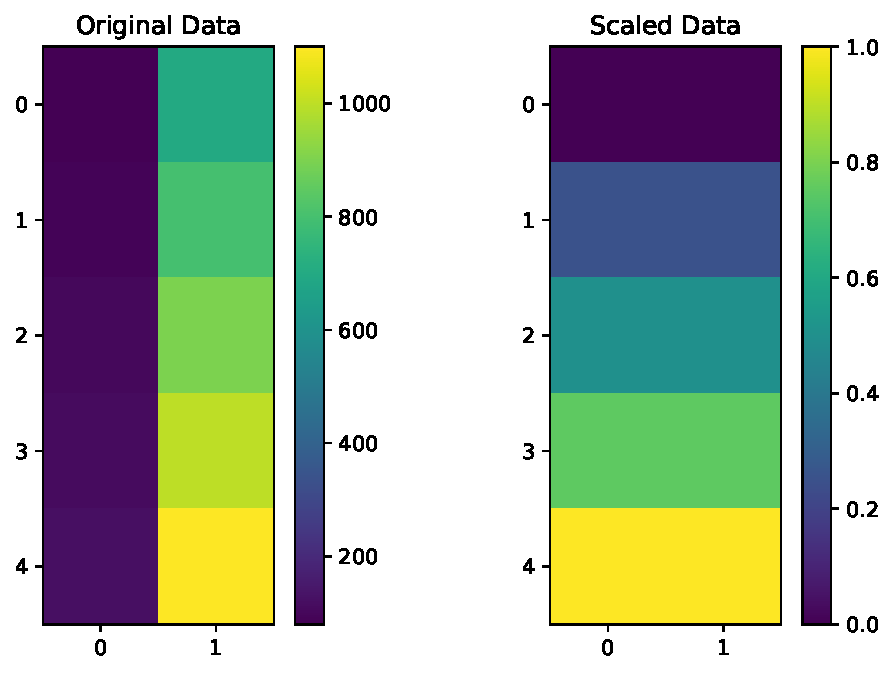
\includegraphics{module_2_files/figure-pdf/fig-totalsales-output-1.pdf}

}

\caption{\label{fig-totalsales}Total sales using \texttt{pandas} method}

\end{figure}%

From the first sub plot, it is clear that there is a significant
difference in the distributions (Metric A and Metric B values). But the
second sub plot shows that both the distributions have same pattern and
the values ranges between 0 and 1. In short the visualization is more
appealing and self explanatory in this case.

\begin{tcolorbox}[enhanced jigsaw, rightrule=.15mm, arc=.35mm, breakable, colback=white, toprule=.15mm, colframe=quarto-callout-note-color-frame, toptitle=1mm, opacityback=0, colbacktitle=quarto-callout-note-color!10!white, opacitybacktitle=0.6, title=\textcolor{quarto-callout-note-color}{\faInfo}\hspace{0.5em}{Note}, bottomrule=.15mm, left=2mm, titlerule=0mm, coltitle=black, bottomtitle=1mm, leftrule=.75mm]

The \texttt{min-max} scaling method will confine the feature values
(attributes) into the range \([0,1]\). So in effect all the features are
scaled proportionally to the data spectrum.

\end{tcolorbox}

Similarly, we can use the \texttt{standard\ scaling} (transformation to
normal distribution) using the transformation
\(\dfrac{x-\bar{x}}{\sigma}\). Scaling table is given as a practice task
to the reader. The python code for this operation is shown in
Fig~\ref{fig-minmax}.

\begin{Shaded}
\begin{Highlighting}[]
\CommentTok{\# Standard scaling from scratch}
\KeywordTok{def}\NormalTok{ standard\_scaling(data):}
\NormalTok{    mean }\OperatorTok{=}\NormalTok{ np.mean(data, axis}\OperatorTok{=}\DecValTok{0}\NormalTok{)}
\NormalTok{    std }\OperatorTok{=}\NormalTok{ np.std(data, axis}\OperatorTok{=}\DecValTok{0}\NormalTok{)}
\NormalTok{    scaled\_data }\OperatorTok{=}\NormalTok{ (data }\OperatorTok{{-}}\NormalTok{ mean) }\OperatorTok{/}\NormalTok{ std}
    \ControlFlowTok{return}\NormalTok{ scaled\_data}

\CommentTok{\# Apply standard scaling}
\NormalTok{scaled\_data\_scratch }\OperatorTok{=}\NormalTok{ standard\_scaling(data)}

\BuiltInTok{print}\NormalTok{(}\StringTok{"Standard Scaled Data (from scratch):}\CharTok{\textbackslash{}n}\StringTok{"}\NormalTok{, scaled\_data\_scratch)}

\CommentTok{\# Visualization}
\NormalTok{plt.figure(figsize}\OperatorTok{=}\NormalTok{(}\DecValTok{6}\NormalTok{, }\DecValTok{5}\NormalTok{))}
\NormalTok{plt.subplot(}\DecValTok{1}\NormalTok{, }\DecValTok{2}\NormalTok{, }\DecValTok{1}\NormalTok{)}
\NormalTok{plt.imshow(data, cmap}\OperatorTok{=}\StringTok{\textquotesingle{}viridis\textquotesingle{}}\NormalTok{)}
\NormalTok{plt.title(}\StringTok{\textquotesingle{}Original Data\textquotesingle{}}\NormalTok{)}
\NormalTok{plt.colorbar()}

\NormalTok{plt.subplot(}\DecValTok{1}\NormalTok{, }\DecValTok{2}\NormalTok{, }\DecValTok{2}\NormalTok{)}
\NormalTok{plt.imshow(scaled\_data\_scratch, cmap}\OperatorTok{=}\StringTok{\textquotesingle{}viridis\textquotesingle{}}\NormalTok{)}
\NormalTok{plt.title(}\StringTok{\textquotesingle{}Scaled Data\textquotesingle{}}\NormalTok{)}
\NormalTok{plt.colorbar()}

\NormalTok{plt.show()}
\end{Highlighting}
\end{Shaded}

\begin{verbatim}
Standard Scaled Data (from scratch):
 [[-1.41421356 -1.41421356]
 [-0.70710678 -0.70710678]
 [ 0.          0.        ]
 [ 0.70710678  0.70710678]
 [ 1.41421356  1.41421356]]
\end{verbatim}

\begin{figure}[H]

\centering{

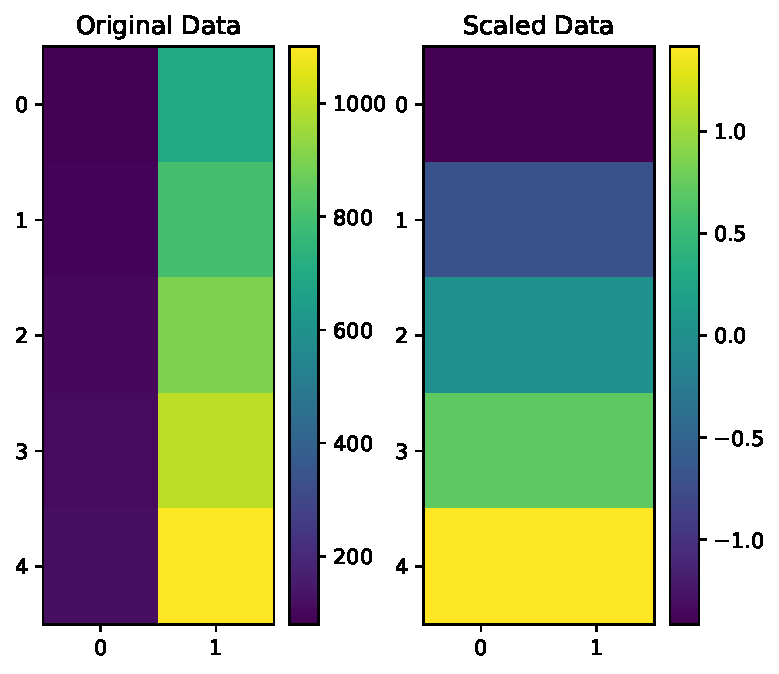
\includegraphics{module_2_files/figure-pdf/fig-minmax-output-2.pdf}

}

\caption{\label{fig-minmax}Min-max scaling using basic python}

\end{figure}%

To understand the effect of standard scaling, let us consider
Fig~\ref{fig-comp1}. This plot create the frequency distribution of the
data as a histogram along with the density function. From the first
sub-plot, it is clear that the distribution has multiple modes (peaks).
When we apply the standard scaling, the distribution become
un-modal(only one peek). This is demonstrated in the second sub-plot.

\begin{Shaded}
\begin{Highlighting}[]
\CommentTok{\# Standard scaling from scratch}
\ImportTok{import}\NormalTok{ seaborn }\ImportTok{as}\NormalTok{ sns}
\CommentTok{\# Create plots}
\NormalTok{plt.figure(figsize}\OperatorTok{=}\NormalTok{(}\DecValTok{6}\NormalTok{, }\DecValTok{5}\NormalTok{))}

\CommentTok{\# Plot for original data}
\NormalTok{plt.subplot(}\DecValTok{1}\NormalTok{, }\DecValTok{2}\NormalTok{, }\DecValTok{1}\NormalTok{)}
\NormalTok{sns.histplot(data, kde}\OperatorTok{=}\VariableTok{True}\NormalTok{, bins}\OperatorTok{=}\DecValTok{10}\NormalTok{, palette}\OperatorTok{=}\StringTok{"viridis"}\NormalTok{)}
\NormalTok{plt.title(}\StringTok{\textquotesingle{}Original Data Distribution\textquotesingle{}}\NormalTok{)}
\NormalTok{plt.xlabel(}\StringTok{\textquotesingle{}Value\textquotesingle{}}\NormalTok{)}
\NormalTok{plt.ylabel(}\StringTok{\textquotesingle{}Frequency\textquotesingle{}}\NormalTok{)}

\CommentTok{\# Plot for standard scaled data}
\NormalTok{plt.subplot(}\DecValTok{1}\NormalTok{, }\DecValTok{2}\NormalTok{, }\DecValTok{2}\NormalTok{)}
\NormalTok{sns.histplot(scaled\_data\_scratch, kde}\OperatorTok{=}\VariableTok{True}\NormalTok{, bins}\OperatorTok{=}\DecValTok{10}\NormalTok{, palette}\OperatorTok{=}\StringTok{"viridis"}\NormalTok{)}
\NormalTok{plt.title(}\StringTok{\textquotesingle{}Standard Scaled Data Distribution\textquotesingle{}}\NormalTok{)}
\NormalTok{plt.xlabel(}\StringTok{\textquotesingle{}Value\textquotesingle{}}\NormalTok{)}
\NormalTok{plt.ylabel(}\StringTok{\textquotesingle{}Frequency\textquotesingle{}}\NormalTok{)}

\NormalTok{plt.tight\_layout()}
\NormalTok{plt.show()}
\end{Highlighting}
\end{Shaded}

\begin{figure}[H]

\centering{

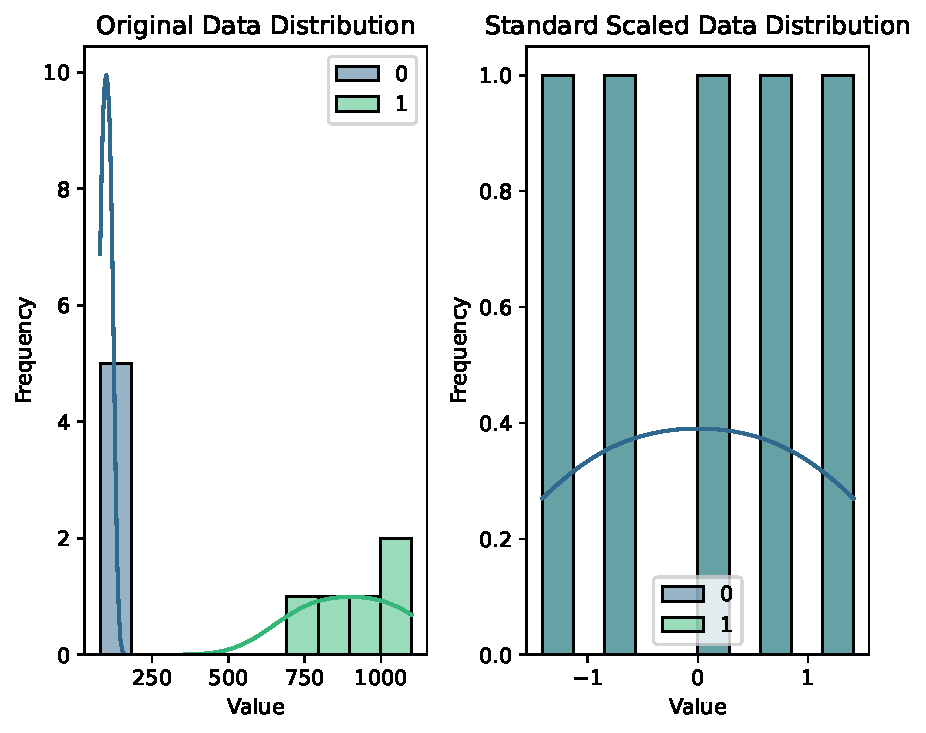
\includegraphics{module_2_files/figure-pdf/fig-comp1-output-1.pdf}

}

\caption{\label{fig-comp1}Impact of standard scaling on the
distribution}

\end{figure}%

A scatter plot showing the compare the impact of scaling on the given
distribution is shown in Fig~\ref{fig-scatter}.

\begin{Shaded}
\begin{Highlighting}[]
\CommentTok{\# Plot original and scaled data}
\NormalTok{plt.figure(figsize}\OperatorTok{=}\NormalTok{(}\DecValTok{6}\NormalTok{, }\DecValTok{5}\NormalTok{))}

\CommentTok{\# Original Data}
\NormalTok{plt.subplot(}\DecValTok{1}\NormalTok{, }\DecValTok{3}\NormalTok{, }\DecValTok{1}\NormalTok{)}
\NormalTok{plt.scatter(data[:, }\DecValTok{0}\NormalTok{], data[:, }\DecValTok{1}\NormalTok{], color}\OperatorTok{=}\StringTok{\textquotesingle{}blue\textquotesingle{}}\NormalTok{)}
\NormalTok{plt.title(}\StringTok{\textquotesingle{}Original Data\textquotesingle{}}\NormalTok{)}
\NormalTok{plt.xlabel(}\StringTok{\textquotesingle{}Metric A\textquotesingle{}}\NormalTok{)}
\NormalTok{plt.ylabel(}\StringTok{\textquotesingle{}Metric B\textquotesingle{}}\NormalTok{)}

\CommentTok{\# Standard Scaled Data}
\NormalTok{plt.subplot(}\DecValTok{1}\NormalTok{, }\DecValTok{3}\NormalTok{, }\DecValTok{2}\NormalTok{)}
\NormalTok{plt.scatter(scaled\_data\_scratch[:, }\DecValTok{0}\NormalTok{], scaled\_data\_scratch[:, }\DecValTok{1}\NormalTok{], color}\OperatorTok{=}\StringTok{\textquotesingle{}green\textquotesingle{}}\NormalTok{)}
\NormalTok{plt.title(}\StringTok{\textquotesingle{}Standard Scaled Data\textquotesingle{}}\NormalTok{)}
\NormalTok{plt.xlabel(}\StringTok{\textquotesingle{}Metric A (Standard Scaled)\textquotesingle{}}\NormalTok{)}
\NormalTok{plt.ylabel(}\StringTok{\textquotesingle{}Metric B (Standard Scaled)\textquotesingle{}}\NormalTok{)}

\CommentTok{\# Min{-}Max Scaled Data}
\NormalTok{plt.subplot(}\DecValTok{1}\NormalTok{, }\DecValTok{3}\NormalTok{, }\DecValTok{3}\NormalTok{)}
\NormalTok{plt.scatter(scaled\_data[:, }\DecValTok{0}\NormalTok{], scaled\_data[:, }\DecValTok{1}\NormalTok{], color}\OperatorTok{=}\StringTok{\textquotesingle{}red\textquotesingle{}}\NormalTok{)}
\NormalTok{plt.title(}\StringTok{\textquotesingle{}Min{-}Max Scaled Data\textquotesingle{}}\NormalTok{)}
\NormalTok{plt.xlabel(}\StringTok{\textquotesingle{}Metric A (Min{-}Max Scaled)\textquotesingle{}}\NormalTok{)}
\NormalTok{plt.ylabel(}\StringTok{\textquotesingle{}Metric B (Min{-}Max Scaled)\textquotesingle{}}\NormalTok{)}

\NormalTok{plt.tight\_layout()}
\NormalTok{plt.show()}
\end{Highlighting}
\end{Shaded}

\begin{figure}[H]

\centering{

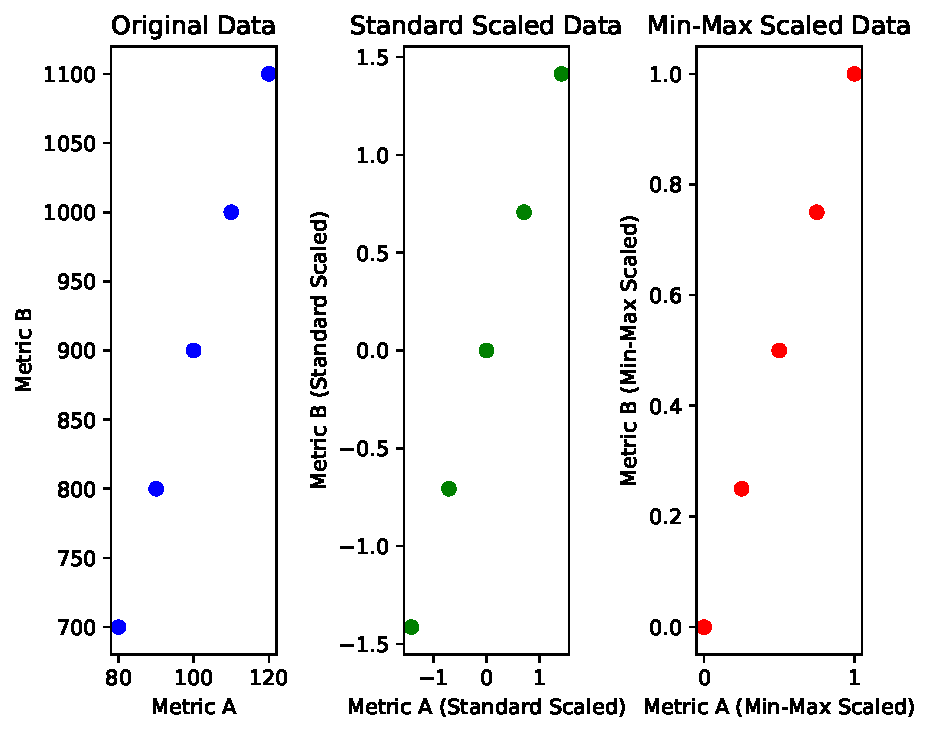
\includegraphics{module_2_files/figure-pdf/fig-scatter-output-1.pdf}

}

\caption{\label{fig-scatter}Comparison of impact of scaling on the
distribution}

\end{figure}%

From the Fig~\ref{fig-scatter}, it is clear that the scaling does not
affect the pattern of the data, instead it just scale the distribution
proportionally!

We can use the \texttt{scikit-learn} library for do the same thing in a
very simple handy approach. The \texttt{python} code for this job is
shown below.

\begin{Shaded}
\begin{Highlighting}[]
\ImportTok{from}\NormalTok{ sklearn.preprocessing }\ImportTok{import}\NormalTok{ MinMaxScaler}

\CommentTok{\# Min{-}max scaling using sklearn}
\NormalTok{scaler }\OperatorTok{=}\NormalTok{ MinMaxScaler()}
\NormalTok{min\_max\_scaled\_data\_sklearn }\OperatorTok{=}\NormalTok{ scaler.fit\_transform(data)}

\BuiltInTok{print}\NormalTok{(}\StringTok{"Min{-}Max Scaled Data (using sklearn):}\CharTok{\textbackslash{}n}\StringTok{"}\NormalTok{, min\_max\_scaled\_data\_sklearn)}
\end{Highlighting}
\end{Shaded}

\begin{verbatim}
Min-Max Scaled Data (using sklearn):
 [[0.   0.  ]
 [0.25 0.25]
 [0.5  0.5 ]
 [0.75 0.75]
 [1.   1.  ]]
\end{verbatim}

\begin{Shaded}
\begin{Highlighting}[]
\ImportTok{from}\NormalTok{ sklearn.preprocessing }\ImportTok{import}\NormalTok{ StandardScaler}

\CommentTok{\# Standard scaling using sklearn}
\NormalTok{scaler }\OperatorTok{=}\NormalTok{ StandardScaler()}
\NormalTok{scaled\_data\_sklearn }\OperatorTok{=}\NormalTok{ scaler.fit\_transform(data)}

\BuiltInTok{print}\NormalTok{(}\StringTok{"Standard Scaled Data (using sklearn):}\CharTok{\textbackslash{}n}\StringTok{"}\NormalTok{, scaled\_data\_sklearn)}
\end{Highlighting}
\end{Shaded}

\begin{verbatim}
Standard Scaled Data (using sklearn):
 [[-1.41421356 -1.41421356]
 [-0.70710678 -0.70710678]
 [ 0.          0.        ]
 [ 0.70710678  0.70710678]
 [ 1.41421356  1.41421356]]
\end{verbatim}

A scatter plot showing the impact on scaling is shown in
Fig~\ref{fig-comp2}. This plot compare the m\texttt{min-max} and
\texttt{standard-scaling}.

\begin{Shaded}
\begin{Highlighting}[]
\CommentTok{\# Plot original and scaled data}
\NormalTok{plt.figure(figsize}\OperatorTok{=}\NormalTok{(}\DecValTok{6}\NormalTok{, }\DecValTok{5}\NormalTok{))}

\CommentTok{\# Original Data}
\NormalTok{plt.subplot(}\DecValTok{1}\NormalTok{, }\DecValTok{3}\NormalTok{, }\DecValTok{1}\NormalTok{)}
\NormalTok{plt.scatter(data[:, }\DecValTok{0}\NormalTok{], data[:, }\DecValTok{1}\NormalTok{], color}\OperatorTok{=}\StringTok{\textquotesingle{}blue\textquotesingle{}}\NormalTok{)}
\NormalTok{plt.title(}\StringTok{\textquotesingle{}Original Data\textquotesingle{}}\NormalTok{)}
\NormalTok{plt.xlabel(}\StringTok{\textquotesingle{}Metric A\textquotesingle{}}\NormalTok{)}
\NormalTok{plt.ylabel(}\StringTok{\textquotesingle{}Metric B\textquotesingle{}}\NormalTok{)}

\CommentTok{\# Standard Scaled Data}
\NormalTok{plt.subplot(}\DecValTok{1}\NormalTok{, }\DecValTok{3}\NormalTok{, }\DecValTok{2}\NormalTok{)}
\NormalTok{plt.scatter(scaled\_data\_sklearn[:, }\DecValTok{0}\NormalTok{], scaled\_data\_sklearn[:, }\DecValTok{1}\NormalTok{], color}\OperatorTok{=}\StringTok{\textquotesingle{}green\textquotesingle{}}\NormalTok{)}
\NormalTok{plt.title(}\StringTok{\textquotesingle{}Standard Scaled Data\textquotesingle{}}\NormalTok{)}
\NormalTok{plt.xlabel(}\StringTok{\textquotesingle{}Metric A (Standard Scaled)\textquotesingle{}}\NormalTok{)}
\NormalTok{plt.ylabel(}\StringTok{\textquotesingle{}Metric B (Standard Scaled)\textquotesingle{}}\NormalTok{)}

\CommentTok{\# Min{-}Max Scaled Data}
\NormalTok{plt.subplot(}\DecValTok{1}\NormalTok{, }\DecValTok{3}\NormalTok{, }\DecValTok{3}\NormalTok{)}
\NormalTok{plt.scatter(min\_max\_scaled\_data\_sklearn[:, }\DecValTok{0}\NormalTok{], min\_max\_scaled\_data\_sklearn[:, }\DecValTok{1}\NormalTok{], color}\OperatorTok{=}\StringTok{\textquotesingle{}red\textquotesingle{}}\NormalTok{)}
\NormalTok{plt.title(}\StringTok{\textquotesingle{}Min{-}Max Scaled Data\textquotesingle{}}\NormalTok{)}
\NormalTok{plt.xlabel(}\StringTok{\textquotesingle{}Metric A (Min{-}Max Scaled)\textquotesingle{}}\NormalTok{)}
\NormalTok{plt.ylabel(}\StringTok{\textquotesingle{}Metric B (Min{-}Max Scaled)\textquotesingle{}}\NormalTok{)}

\NormalTok{plt.tight\_layout()}
\NormalTok{plt.show()}
\end{Highlighting}
\end{Shaded}

\begin{figure}[H]

\centering{

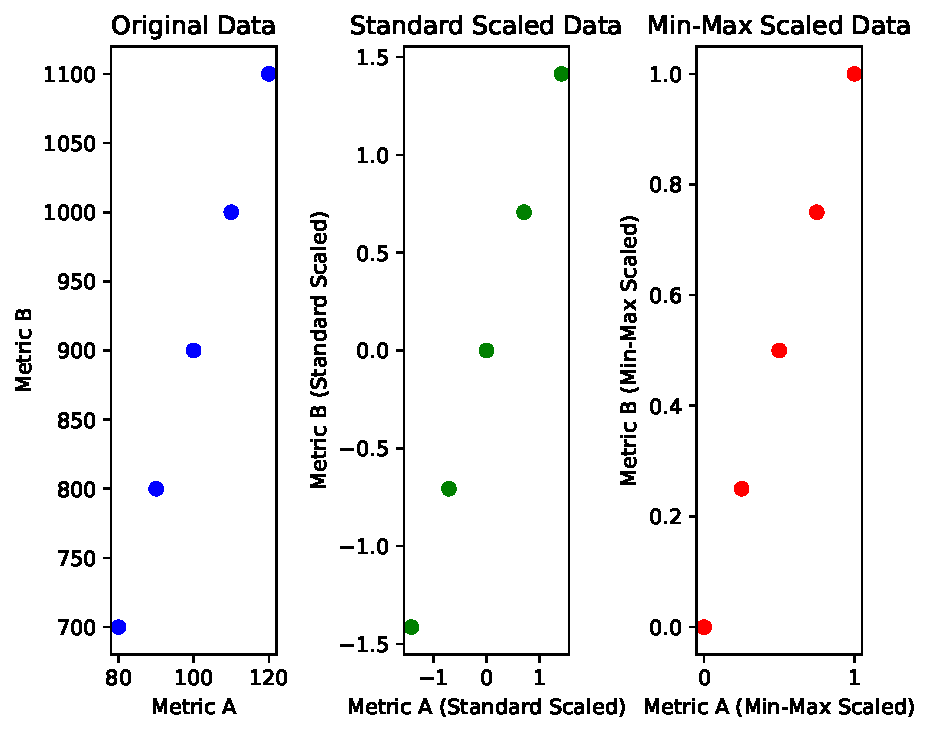
\includegraphics{module_2_files/figure-pdf/fig-comp2-output-1.pdf}

}

\caption{\label{fig-comp2}Camparison of Min-max and standard scalings
with original data}

\end{figure}%

\subsection{More on Matrix Product and its
Applications}\label{more-on-matrix-product-and-its-applications}

In the first module of our course, we introduced matrix products as
scalar projections, focusing on how matrices interact through basic
operations. In this section, we will expand on this by exploring
different types of matrix products that have practical importance in
various fields. One such product is the \emph{Hadamard product}, which
is particularly useful in applications ranging from image processing to
neural networks and statistical analysis. We will cover the definition,
properties, and examples of the Hadamard product, and then delve into
practical applications with simulated data.

\subsubsection{Hadamard Product}\label{hadamard-product}

The Hadamard product (or element-wise product) of two matrices is a
binary operation that combines two matrices of the same dimensions to
produce another matrix of the same dimensions, where each element is the
product of corresponding elements in the original matrices.

\begin{tcolorbox}[enhanced jigsaw, rightrule=.15mm, arc=.35mm, breakable, colback=white, toprule=.15mm, colframe=quarto-callout-important-color-frame, toptitle=1mm, opacityback=0, colbacktitle=quarto-callout-important-color!10!white, opacitybacktitle=0.6, title=\textcolor{quarto-callout-important-color}{\faExclamation}\hspace{0.5em}{Definition (Hadamard Product):}, bottomrule=.15mm, left=2mm, titlerule=0mm, coltitle=black, bottomtitle=1mm, leftrule=.75mm]

For two matrices \(A\) and \(B\) of the same dimension \(m \times n\),
the Hadamard product \(A \circ B\) is defined as:

\[(A \circ B)_{ij} = A_{ij} \cdot B_{ij}\]

where \(\cdot\) denotes element-wise multiplication.

\end{tcolorbox}

\begin{tcolorbox}[enhanced jigsaw, rightrule=.15mm, arc=.35mm, breakable, colback=white, toprule=.15mm, colframe=quarto-callout-note-color-frame, toptitle=1mm, opacityback=0, colbacktitle=quarto-callout-note-color!10!white, opacitybacktitle=0.6, title=\textcolor{quarto-callout-note-color}{\faInfo}\hspace{0.5em}{Properties of Hadamard Product}, bottomrule=.15mm, left=2mm, titlerule=0mm, coltitle=black, bottomtitle=1mm, leftrule=.75mm]

\begin{enumerate}
\def\labelenumi{\arabic{enumi}.}
\item
  \textbf{Commutativity}: \[A \circ B = B \circ A\]
\item
  \textbf{Associativity}: \[(A \circ B) \circ C = A \circ (B \circ C)\]
\item
  \textbf{Distributivity}:
  \[A \circ (B + C) = (A \circ B) + (A \circ C)\]
\end{enumerate}

\end{tcolorbox}

Some simple examples to demonstrate the Hadamard product is given below.

Example 1: Basic Hadamard Product

Given matrices:

\[A = \begin{pmatrix}1 & 2 \\3 & 4\end{pmatrix}, \quad B = \begin{pmatrix}5 & 6 \\7 & 8\end{pmatrix}\]

The Hadamard product \(A \circ B\) is:

\[A \circ B = \begin{pmatrix}1 \cdot 5 & 2 \cdot 6 \\3 \cdot 7 & 4 \cdot 8\end{pmatrix} = \begin{pmatrix}5 & 12 \\21 & 32\end{pmatrix}\]

Example 2: Hadamard Product with Larger Matrices

Given matrices:

\[A = \begin{pmatrix}1 & 2 & 3 \\4 & 5 & 6 \\7 & 8 & 9\end{pmatrix}, \quad B = \begin{pmatrix}9 & 8 & 7 \\6 & 5 & 4 \\3 & 2 & 1\end{pmatrix}\]

The Hadamard product \(A \circ B\) is:

\[A \circ B = \begin{pmatrix}1 \cdot 9 & 2 \cdot 8 & 3 \cdot 7 \\4 \cdot 6 & 5 \cdot 5 & 6 \cdot 4 \\7 \cdot 3 & 8 \cdot  & 9 \cdot 1\end{pmatrix} = \begin{pmatrix}9 & 16 & 21 \\24 & 25 & 24 \\21 & 16 & 9\end{pmatrix}\]

In the following code chunks the computational process of Hadamard
product is implemented in \texttt{Python}. Here both the from the
scratch and use of external module versions are included.

\textbf{1. Compute Hadamard Product from Scratch (without Libraries)}

Here's how you can compute the Hadamard product manually:

\begin{Shaded}
\begin{Highlighting}[]
\CommentTok{\# Define matrices A and B}
\NormalTok{A }\OperatorTok{=}\NormalTok{ [[}\DecValTok{1}\NormalTok{, }\DecValTok{2}\NormalTok{, }\DecValTok{3}\NormalTok{], [}\DecValTok{4}\NormalTok{, }\DecValTok{5}\NormalTok{, }\DecValTok{6}\NormalTok{]]}
\NormalTok{B }\OperatorTok{=}\NormalTok{ [[}\DecValTok{7}\NormalTok{, }\DecValTok{8}\NormalTok{, }\DecValTok{9}\NormalTok{], [}\DecValTok{10}\NormalTok{, }\DecValTok{11}\NormalTok{, }\DecValTok{12}\NormalTok{]]}

\CommentTok{\# Function to compute Hadamard product}
\KeywordTok{def}\NormalTok{ hadamard\_product(A, B):}
    \CommentTok{\# Get the number of rows and columns}
\NormalTok{    num\_rows }\OperatorTok{=} \BuiltInTok{len}\NormalTok{(A)}
\NormalTok{    num\_cols }\OperatorTok{=} \BuiltInTok{len}\NormalTok{(A[}\DecValTok{0}\NormalTok{])}
    
    \CommentTok{\# Initialize the result matrix}
\NormalTok{    result }\OperatorTok{=}\NormalTok{ [[}\DecValTok{0}\NormalTok{]}\OperatorTok{*}\NormalTok{num\_cols }\ControlFlowTok{for}\NormalTok{ \_ }\KeywordTok{in} \BuiltInTok{range}\NormalTok{(num\_rows)]}
    
    \CommentTok{\# Compute the Hadamard product}
    \ControlFlowTok{for}\NormalTok{ i }\KeywordTok{in} \BuiltInTok{range}\NormalTok{(num\_rows):}
        \ControlFlowTok{for}\NormalTok{ j }\KeywordTok{in} \BuiltInTok{range}\NormalTok{(num\_cols):}
\NormalTok{            result[i][j] }\OperatorTok{=}\NormalTok{ A[i][j] }\OperatorTok{*}\NormalTok{ B[i][j]}
    
    \ControlFlowTok{return}\NormalTok{ result}

\CommentTok{\# Compute Hadamard product}
\NormalTok{hadamard\_product\_result }\OperatorTok{=}\NormalTok{ hadamard\_product(A, B)}

\CommentTok{\# Display result}
\BuiltInTok{print}\NormalTok{(}\StringTok{"Hadamard Product (From Scratch):"}\NormalTok{)}
\ControlFlowTok{for}\NormalTok{ row }\KeywordTok{in}\NormalTok{ hadamard\_product\_result:}
    \BuiltInTok{print}\NormalTok{(row)}
\end{Highlighting}
\end{Shaded}

\begin{verbatim}
Hadamard Product (From Scratch):
[7, 16, 27]
[40, 55, 72]
\end{verbatim}

\textbf{2. Compute Hadamard Product Using \texttt{SymPy}}

Here's how to compute the Hadamard product using \texttt{SymPy}:

\begin{Shaded}
\begin{Highlighting}[]
\ImportTok{import}\NormalTok{ sympy }\ImportTok{as}\NormalTok{ sp}

\CommentTok{\# Define matrices A and B}
\NormalTok{A }\OperatorTok{=}\NormalTok{ sp.Matrix([[}\DecValTok{1}\NormalTok{, }\DecValTok{2}\NormalTok{, }\DecValTok{3}\NormalTok{], [}\DecValTok{4}\NormalTok{, }\DecValTok{5}\NormalTok{, }\DecValTok{6}\NormalTok{]])}
\NormalTok{B }\OperatorTok{=}\NormalTok{ sp.Matrix([[}\DecValTok{7}\NormalTok{, }\DecValTok{8}\NormalTok{, }\DecValTok{9}\NormalTok{], [}\DecValTok{10}\NormalTok{, }\DecValTok{11}\NormalTok{, }\DecValTok{12}\NormalTok{]])}

\CommentTok{\# Compute Hadamard product using SymPy}
\NormalTok{Hadamard\_product\_sympy }\OperatorTok{=}\NormalTok{ A.multiply\_elementwise(B)}

\CommentTok{\# Display result}
\BuiltInTok{print}\NormalTok{(}\StringTok{"Hadamard Product (Using SymPy):"}\NormalTok{)}
\BuiltInTok{print}\NormalTok{(Hadamard\_product\_sympy)}
\end{Highlighting}
\end{Shaded}

\begin{verbatim}
Hadamard Product (Using SymPy):
Matrix([[7, 16, 27], [40, 55, 72]])
\end{verbatim}

\textbf{Practical Applications}

\emph{Application 1: Image Masking}

The Hadamard product can be used for image masking. Here's how you can
apply a mask to an image and visualize it as shown in
Fig~\ref{fig-imgmask}.

\begin{Shaded}
\begin{Highlighting}[]
\ImportTok{import}\NormalTok{ matplotlib.pyplot }\ImportTok{as}\NormalTok{ plt}
\ImportTok{import}\NormalTok{ numpy }\ImportTok{as}\NormalTok{ np}

\CommentTok{\# Simulated large image (2D array) using NumPy}
\NormalTok{image }\OperatorTok{=}\NormalTok{ np.random.rand(}\DecValTok{100}\NormalTok{, }\DecValTok{100}\NormalTok{)}

\CommentTok{\# Simulated mask (binary matrix) using NumPy}
\NormalTok{mask }\OperatorTok{=}\NormalTok{ np.random.randint(}\DecValTok{0}\NormalTok{, }\DecValTok{2}\NormalTok{, size}\OperatorTok{=}\NormalTok{(}\DecValTok{100}\NormalTok{, }\DecValTok{100}\NormalTok{))}

\CommentTok{\# Compute Hadamard product}
\NormalTok{masked\_image }\OperatorTok{=}\NormalTok{ image }\OperatorTok{*}\NormalTok{ mask}

\CommentTok{\# Plot original image and masked image}
\NormalTok{fig, ax }\OperatorTok{=}\NormalTok{ plt.subplots(}\DecValTok{1}\NormalTok{, }\DecValTok{2}\NormalTok{, figsize}\OperatorTok{=}\NormalTok{(}\DecValTok{12}\NormalTok{, }\DecValTok{5}\NormalTok{))}
\NormalTok{ax[}\DecValTok{0}\NormalTok{].imshow(image, cmap}\OperatorTok{=}\StringTok{\textquotesingle{}gray\textquotesingle{}}\NormalTok{)}
\NormalTok{ax[}\DecValTok{0}\NormalTok{].set\_title(}\StringTok{\textquotesingle{}Original Image\textquotesingle{}}\NormalTok{)}
\NormalTok{ax[}\DecValTok{1}\NormalTok{].imshow(masked\_image, cmap}\OperatorTok{=}\StringTok{\textquotesingle{}gray\textquotesingle{}}\NormalTok{)}
\NormalTok{ax[}\DecValTok{1}\NormalTok{].set\_title(}\StringTok{\textquotesingle{}Masked Image\textquotesingle{}}\NormalTok{)}
\NormalTok{plt.show()}
\end{Highlighting}
\end{Shaded}

\begin{figure}[H]

\centering{

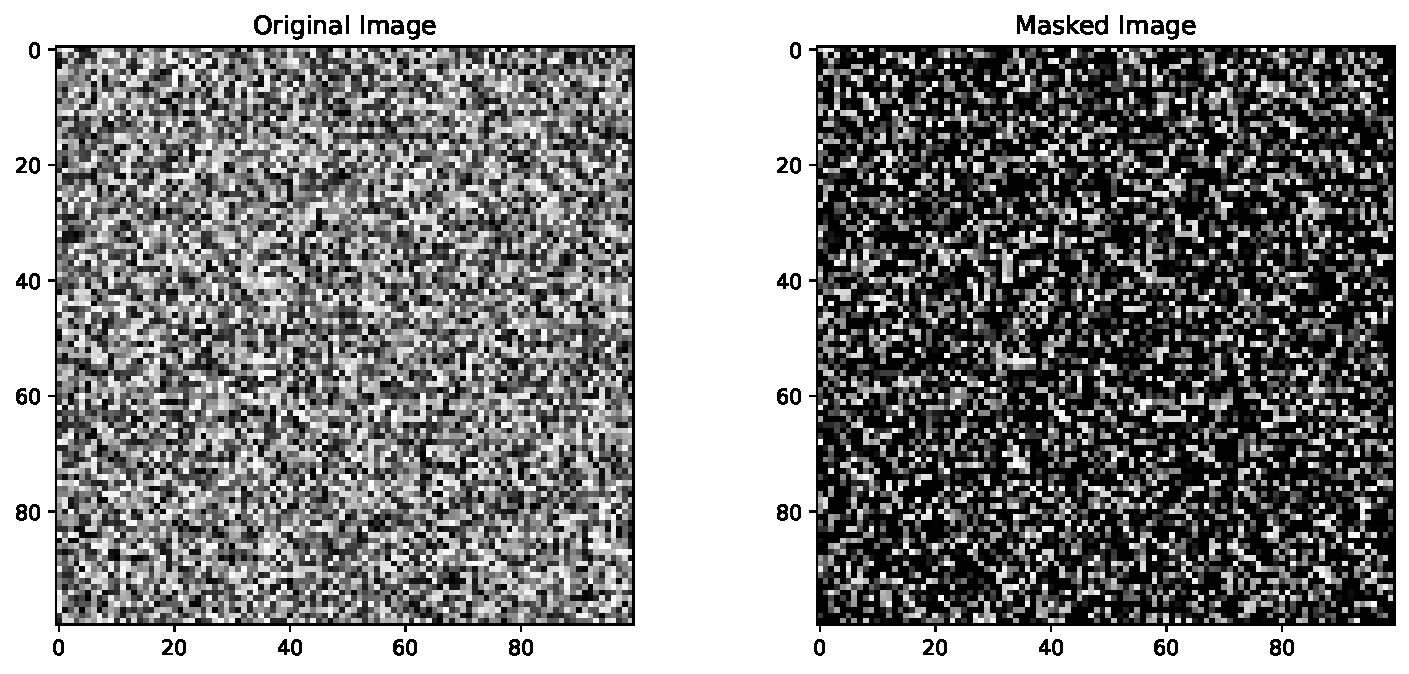
\includegraphics{module_2_files/figure-pdf/fig-imgmask-output-1.pdf}

}

\caption{\label{fig-imgmask}Demonstration of Masking in DIP using
Hadamard Product}

\end{figure}%

Application 2: Element-wise Scaling in Neural Networks

The Hadamard product can be used for dropout\footnote{A regularization
  techniques in Deep learning. This approach deactivate some selected
  neurons to control model over-fitting} in neural networks. A simple
simulated example is given below.

\begin{Shaded}
\begin{Highlighting}[]
\CommentTok{\# Simulated large activations (2D array) using NumPy}
\NormalTok{activations }\OperatorTok{=}\NormalTok{ np.random.rand(}\DecValTok{100}\NormalTok{, }\DecValTok{100}\NormalTok{)}

\CommentTok{\# Simulated dropout mask (binary matrix) using NumPy}
\NormalTok{dropout\_mask }\OperatorTok{=}\NormalTok{ np.random.randint(}\DecValTok{0}\NormalTok{, }\DecValTok{2}\NormalTok{, size}\OperatorTok{=}\NormalTok{(}\DecValTok{100}\NormalTok{, }\DecValTok{100}\NormalTok{))}

\CommentTok{\# Apply dropout}
\NormalTok{dropped\_activations }\OperatorTok{=}\NormalTok{ activations }\OperatorTok{*}\NormalTok{ dropout\_mask}

\CommentTok{\# Display results}
\BuiltInTok{print}\NormalTok{(}\StringTok{"Original Activations:"}\NormalTok{)}
\BuiltInTok{print}\NormalTok{(activations)}
\BuiltInTok{print}\NormalTok{(}\StringTok{"}\CharTok{\textbackslash{}n}\StringTok{Dropout Mask:"}\NormalTok{)}
\BuiltInTok{print}\NormalTok{(dropout\_mask)}
\BuiltInTok{print}\NormalTok{(}\StringTok{"}\CharTok{\textbackslash{}n}\StringTok{Dropped Activations:"}\NormalTok{)}
\BuiltInTok{print}\NormalTok{(dropped\_activations)}
\end{Highlighting}
\end{Shaded}

\begin{verbatim}
Original Activations:
[[0.1007953  0.48719122 0.24592139 ... 0.03832734 0.07613249 0.92387318]
 [0.25298548 0.55918157 0.52303492 ... 0.68604885 0.92870841 0.86914188]
 [0.96578376 0.88008027 0.9262686  ... 0.77042725 0.99727931 0.20447267]
 ...
 [0.96250255 0.87429133 0.9244299  ... 0.07194137 0.81818265 0.85395391]
 [0.47783031 0.63289769 0.1947535  ... 0.22386757 0.71172666 0.27496288]
 [0.98374551 0.98972032 0.97459696 ... 0.11221483 0.09372771 0.94129436]]

Dropout Mask:
[[0 1 1 ... 0 1 0]
 [0 0 1 ... 1 1 1]
 [1 1 0 ... 0 1 1]
 ...
 [1 1 1 ... 0 0 0]
 [1 0 0 ... 1 0 1]
 [0 1 0 ... 0 1 0]]

Dropped Activations:
[[0.         0.48719122 0.24592139 ... 0.         0.07613249 0.        ]
 [0.         0.         0.52303492 ... 0.68604885 0.92870841 0.86914188]
 [0.96578376 0.88008027 0.         ... 0.         0.99727931 0.20447267]
 ...
 [0.96250255 0.87429133 0.9244299  ... 0.         0.         0.        ]
 [0.47783031 0.         0.         ... 0.22386757 0.         0.27496288]
 [0.         0.98972032 0.         ... 0.         0.09372771 0.        ]]
\end{verbatim}

Application 3: Statistical Data Analysis

In statistics, the Hadamard product can be applied to scale covariance
matrices. Here's how we can compute the covariance matrix using matrix
operations and apply scaling. Following \texttt{Python} code demonstrate
this.

\begin{Shaded}
\begin{Highlighting}[]
\ImportTok{import}\NormalTok{ sympy }\ImportTok{as}\NormalTok{ sp}
\ImportTok{import}\NormalTok{ numpy }\ImportTok{as}\NormalTok{ np}

\CommentTok{\# Simulated large dataset (2D array) using NumPy}
\NormalTok{data }\OperatorTok{=}\NormalTok{ np.random.rand(}\DecValTok{100}\NormalTok{, }\DecValTok{10}\NormalTok{)}

\CommentTok{\# Compute the mean of each column}
\NormalTok{mean }\OperatorTok{=}\NormalTok{ np.mean(data, axis}\OperatorTok{=}\DecValTok{0}\NormalTok{)}

\CommentTok{\# Center the data}
\NormalTok{centered\_data }\OperatorTok{=}\NormalTok{ data }\OperatorTok{{-}}\NormalTok{ mean}

\CommentTok{\# Compute the covariance matrix using matrix product operation}
\NormalTok{cov\_matrix }\OperatorTok{=}\NormalTok{ (centered\_data.T }\OperatorTok{@}\NormalTok{ centered\_data) }\OperatorTok{/}\NormalTok{ (centered\_data.shape[}\DecValTok{0}\NormalTok{] }\OperatorTok{{-}} \DecValTok{1}\NormalTok{)}
\NormalTok{cov\_matrix\_sympy }\OperatorTok{=}\NormalTok{ sp.Matrix(cov\_matrix)}

\CommentTok{\# Simulated scaling factors (2D array) using SymPy Matrix}
\NormalTok{scaling\_factors }\OperatorTok{=}\NormalTok{ sp.Matrix(np.random.rand(}\DecValTok{10}\NormalTok{, }\DecValTok{10}\NormalTok{))}

\CommentTok{\# Compute Hadamard product}
\NormalTok{scaled\_cov\_matrix }\OperatorTok{=}\NormalTok{ cov\_matrix\_sympy.multiply(scaling\_factors)}

\CommentTok{\# Display results}
\BuiltInTok{print}\NormalTok{(}\StringTok{"Covariance Matrix:"}\NormalTok{)}
\BuiltInTok{print}\NormalTok{(cov\_matrix\_sympy)}
\BuiltInTok{print}\NormalTok{(}\StringTok{"}\CharTok{\textbackslash{}n}\StringTok{Scaling Factors:"}\NormalTok{)}
\BuiltInTok{print}\NormalTok{(scaling\_factors)}
\BuiltInTok{print}\NormalTok{(}\StringTok{"}\CharTok{\textbackslash{}n}\StringTok{Scaled Covariance Matrix:"}\NormalTok{)}
\BuiltInTok{print}\NormalTok{(scaled\_cov\_matrix)}
\end{Highlighting}
\end{Shaded}

\begin{verbatim}
Covariance Matrix:
Matrix([[0.0922379146366976, -0.00976709252586460, 0.0114116609529477, -0.00517600912096788, 0.0122097012859354, -0.00515294750757037, -0.00935445065763178, 0.0121090852373357, 0.0100914437950009, 0.0111033100525211], [-0.00976709252586460, 0.0797585884407984, 0.00263029018392435, -0.00907423965997043, -0.000132765049808362, -0.00543740560500525, 0.00320443497522094, -0.00829840306153171, 0.00351621236729423, 0.00975615494983111], [0.0114116609529477, 0.00263029018392435, 0.0900429767034669, 0.00107353021610307, -0.00342974358337094, 0.00712233971622679, 0.00167547412871273, 0.00740235324421338, 0.00650723416792581, 0.00124478129466236], [-0.00517600912096788, -0.00907423965997043, 0.00107353021610307, 0.0929441843970454, 0.0122309693376691, -0.00891048997209941, 0.00676964168924556, -0.0142016440502977, 0.00271402940561709, -0.00529229614566176], [0.0122097012859354, -0.000132765049808362, -0.00342974358337094, 0.0122309693376691, 0.0737220423520933, 0.00937991756689368, -0.00124175152541520, 0.00428794804268919, -0.00414810463654336, 0.0102084391380566], [-0.00515294750757037, -0.00543740560500525, 0.00712233971622679, -0.00891048997209941, 0.00937991756689368, 0.0876113884607199, -0.0106505967931530, -0.00225667918361245, 0.00808654683636813, -0.000995589093019014], [-0.00935445065763178, 0.00320443497522094, 0.00167547412871273, 0.00676964168924556, -0.00124175152541520, -0.0106505967931530, 0.0772752246094700, 0.00592598396114498, -0.000520503051019692, -0.00461519981313001], [0.0121090852373357, -0.00829840306153171, 0.00740235324421338, -0.0142016440502977, 0.00428794804268919, -0.00225667918361245, 0.00592598396114498, 0.0805619757641007, -0.00264247303792696, -0.0222547249604951], [0.0100914437950009, 0.00351621236729423, 0.00650723416792581, 0.00271402940561709, -0.00414810463654336, 0.00808654683636813, -0.000520503051019692, -0.00264247303792696, 0.0819296741707754, 0.00440522173009907], [0.0111033100525211, 0.00975615494983111, 0.00124478129466236, -0.00529229614566176, 0.0102084391380566, -0.000995589093019014, -0.00461519981313001, -0.0222547249604951, 0.00440522173009907, 0.0845777902787088]])

Scaling Factors:
Matrix([[0.965518770491802, 0.522123361002768, 0.484619509813199, 0.802383237899632, 0.580841530252410, 0.670758661504766, 0.969126215532161, 0.125406526616254, 0.547486950909253, 0.341257830270760], [0.444100646285325, 0.874174284511555, 0.578383014644058, 0.700459512330854, 0.545183692718459, 0.700028232470651, 0.0126278956270661, 0.574098994770229, 0.0996428673286411, 0.0364605735796198], [0.239647718935905, 0.727908754585243, 0.432324268237795, 0.346416258480508, 0.823371283385288, 0.846142725400600, 0.879929057585733, 0.441611605375608, 0.316836282221275, 0.686432492753615], [0.112746359950867, 0.311144524742372, 0.770150068778636, 0.398263361923193, 0.756542563389511, 0.874780753862866, 0.778183121113814, 0.831241916575416, 0.129609938097122, 0.952211333939139], [0.960220197041355, 0.877144596772967, 0.0103645704443167, 0.904222971758231, 0.337852012397866, 0.763534601784246, 0.402644880295197, 0.771378100368135, 0.735491556195428, 0.770482772429741], [0.320166868672737, 0.750029016443758, 0.630788048905561, 0.291633686342178, 0.124971724535679, 0.221347517316274, 0.752267419295383, 0.377224680358194, 0.988902479208956, 0.562038617863829], [0.0172056879092415, 0.482150061409474, 0.145913907335095, 0.506096871108297, 0.370319039800190, 0.716194795928193, 0.409398470475934, 0.874169339526082, 0.584656957123496, 0.110642540999108], [0.231562367470364, 0.817892134647635, 0.466725364154612, 0.109433020506892, 0.386660906093796, 0.553328307633047, 0.517279237466910, 0.794474884338932, 0.0751547836443156, 0.216598472884146], [0.676600112162640, 0.996354369455508, 0.941682444956854, 0.767386239200211, 0.115869987291861, 0.648042446149840, 0.784200102441548, 0.162437703715434, 0.330757541334665, 0.397414149663206], [0.892947134339148, 0.0952617153958398, 0.813938350106629, 0.573764937105987, 0.690038546635843, 0.187533195668101, 0.104063362787849, 0.509268513275933, 0.859856666043168, 0.572270889681409]])

Scaled Covariance Matrix:
Matrix([[0.116330866449071, 0.0696684543515319, 0.0597015554544676, 0.0893035937963723, 0.0672610001243607, 0.0769647115556121, 0.107823431266601, 0.0229082291755514, 0.0646809565065246, 0.0524890790058494], [0.0329537611853764, 0.0587104264868263, 0.0399616352488483, 0.0526318366975939, 0.0375037704807356, 0.0440761216446252, -0.0165571823531611, 0.0377776249430564, 0.00758430614738537, -0.00488077382051261], [0.0401301985505233, 0.0899325489389705, 0.0621035754450972, 0.0489604852468134, 0.0878402766201518, 0.0953281446167603, 0.104883854988153, 0.0526752037005788, 0.0444571493677635, 0.0732684809191026], [0.00453903993832599, 0.0169592785576490, 0.0514021086694053, 0.0362579361557980, 0.0599435680945152, 0.0775130555725445, 0.0633659704936832, 0.0703286379485762, 0.00807047784485916, 0.0872808405094513], [0.0933598852670699, 0.0790159303483302, 0.0266809761840964, 0.0852983978627013, 0.0472898949169684, 0.0749693197116204, 0.0545901529536194, 0.0773593351075839, 0.0776698130942699, 0.0805122846805137], [0.0342457917194407, 0.0698881950641711, 0.0501333509507283, 0.0250043022384221, 0.00271700944989097, 0.0137006572626100, 0.0646648053384100, 0.0219585915997521, 0.0866988034850643, 0.0518924089432407], [-0.0128178467584187, 0.0333123470105814, 0.00632159049436127, 0.0304961222346533, 0.0287269167705742, 0.0574229723966298, 0.0230183547850370, 0.0718828967940490, 0.0266447170094973, 0.00456347707215345], [0.00867074876554079, 0.0661015922816657, 0.00981507622287372, 0.00104935409514066, 0.0167085831082128, 0.0418632124058598, 0.0468323977221896, 0.0480966827933208, -0.00326114258982444, 0.00174283364857184], [0.0705228258066870, 0.0959889656268927, 0.0963136339859047, 0.0773494454364063, 0.0261172739114887, 0.0678184115083570, 0.0852029254981186, 0.0212620825935277, 0.0436185092625722, 0.0464230488581998], [0.0975096901465657, 0.0138118560201253, 0.0688929228882828, 0.0701438811885234, 0.0606719912703687, 0.0213713770294315, 0.0100767404771427, 0.0327160567866666, 0.0830941659464219, 0.0520868752913716]])
\end{verbatim}

\subsubsection{Practice Problems}\label{practice-problems-1}

\textbf{Problem 1: Basic Hadamard Product}

Given matrices: \[A=\begin{bmatrix}1&2\\3&4\end{bmatrix}\]
\[B=\begin{bmatrix}5&6\\7&8\end{bmatrix}\]

Find the Hadamard product \(C=A\circ B\).

\textbf{Solution:}

\[C=\begin{bmatrix}1\cdot 5&2\cdot 6\\3\cdot7&4\cdot 8 \end{bmatrix}=\begin{bmatrix}5&12\\21&32\end{bmatrix}\]

\textbf{Problem 2: Hadamard Product with Identity Matrix}

Given matrices: \[A=\begin{bmatrix}1&2&3\\4&5&6\end{bmatrix}\]
\[I=\begin{bmatrix}1&0&0\\0&1&0\end{bmatrix}\]

Find the Hadamard product \(C=A\circ I\).

\textbf{Solution:}

\[C=\begin{bmatrix}1\cdot1&2\cdot 0&3\cdot 0\\4\cdot 0&5\cdot 1&6\cdot 0 \end{bmatrix}= \begin{bmatrix} 1&0&0\\0&5&0\end{bmatrix}\]

\textbf{Problem 3: Hadamard Product with Zero Matrix}

Given matrices: \[A=\begin{bmatrix}3&4\\5&6\end{bmatrix}\]
\[Z=\begin{bmatrix}0&0\\0&0\end{bmatrix}\]

Find the Hadamard product \(C=A\circ Z\).

\textbf{Solution:}

\[C=\begin{bmatrix}3\cdot 0&4\cdot 0\\ 5\cdot 0&6\cdot 0 \end{bmatrix}=\begin{bmatrix}0&0\\0&0\end{bmatrix}\]

\textbf{Problem 4: Hadamard Product of Two Identity Matrices}

Given identity matrices: \[I_2=\begin{bmatrix}1&0\\0&1\end{bmatrix}\]
\[I_3=\begin{bmatrix}1&0&0\\0&1&0\\0&0&1\end{bmatrix}\]

Find the Hadamard product \(C=I_2\circ I_3\) (extend \(I_2\) to match
dimensions of \(I_3\)).

\textbf{Solution:}

Extend \(I_2\) to \(I_3\):
\[I_2=\begin{bmatrix}1&0&0\\0&1&0\\0&0&0\end{bmatrix}\]

\[C=\begin{bmatrix}1\cdot 1&0\cdot 0&0\cdot 0\\0\cdot 0&1\cdot 1&0\cdot 0\\0\cdot 0&0\cdot 0&0\cdot 1\end{bmatrix}=\begin{bmatrix}1&0&0\\0&1&0\\0&0&0\end{bmatrix}\]

\textbf{Problem 5: Hadamard Product with Random Matrices}

Given random matrices: \[A=\begin{bmatrix}2&3\\1&4\end{bmatrix}\]
\[B=\begin{bmatrix}0&5\\6&2\end{bmatrix}\]

Find the Hadamard product \(C=A\circ B\).

\textbf{Solution:}

\[C=\begin{bmatrix}2\cdot 0&3\cdot 5\\1\cdot 6&4\cdot 2\end{bmatrix}=\begin{bmatrix}0&15\\6&8\end{bmatrix}\]

\textbf{Problem 6: Hadamard Product of 3x3 Matrices}

Given matrices: \[A=\begin{bmatrix}1&2&3\\4&5&6\\7&8&9\end{bmatrix}\]
\[B=\begin{bmatrix}9&8&7\\6&5&4\\3&2&1\end{bmatrix}\]

Find the Hadamard product \(C=A\circ B\).

\textbf{Solution:}

\[C=\begin{bmatrix}1\cdot 9&2\cdot 8&3\cdot 7\\4\cdot 6&5\cdot 5&6\cdot 4\\7\cdot 3&8\cdot 2&9\cdot 1\end{bmatrix}=\begin{bmatrix}9&16&21\\24&25&24\\21&16&9\end{bmatrix}\]

\textbf{Problem 7: Hadamard Product of Column Vectors}

Given column vectors: \[u=\begin{bmatrix}2\\3\end{bmatrix}\]
\[v=\begin{bmatrix}5\\6\end{bmatrix}\]

Find the Hadamard product \(w=u\circ v\).

\textbf{Solution:}

\[w=\begin{bmatrix}2\cdot 5\\3\cdot 6\end{bmatrix}=\begin{bmatrix}10\\18\end{bmatrix}\]

\textbf{Problem 8: Hadamard Product with Non-Square Matrices}

Given matrices: \[A=\begin{bmatrix}1&2\\3&4\\5&6\end{bmatrix}\]
\[B=\begin{bmatrix}7&8\\9&10\end{bmatrix}\]

Find the Hadamard product \(C=A\circ B\) (extend \(B\) to match
dimensions of \(A\)).

\textbf{Solution:}

Extend \(B\) to match dimensions of \(A\):
\[B=\begin{bmatrix}7&8\\9&10\\7&8\end{bmatrix}\]

\[C=\begin{bmatrix}1\cdot 7&2\cdot 8\\3\cdot 9&4\cdot 10\\5\cdot 7&6\cdot 8\end{bmatrix}=\begin{bmatrix}7&16\\27&40\\35&48\end{bmatrix}\]

\textbf{Problem 9: Hadamard Product in Image Processing}

Given matrices representing image pixel values:
\[A=\begin{bmatrix}10&20\\30&40\end{bmatrix}\]
\[B=\begin{bmatrix}0.5&1.5\\2.0&0.5\end{bmatrix}\]

Find the Hadamard product \(C=A\circ B\).

\textbf{Solution:}

\[C=\begin{bmatrix}10\cdot 0.5&20\cdot 1.5\\30\cdot 2.0&40\cdot 0.5\end{bmatrix}=\begin{bmatrix}5&30\\60&20\end{bmatrix}\]

\textbf{Problem 10: Hadamard Product in Statistical Data}

Given matrices representing two sets of statistical data:

\[A=\begin{bmatrix}5&6&7\\8&9&10\end{bmatrix}\]
\[B=\begin{bmatrix}1&2&3\\4&5&6\end{bmatrix}\]

Find the Hadamard product \(C=A\circ B\).

\textbf{Solution:}

\[C=\begin{bmatrix}5\cdot 1&6\cdot 2&7\cdot 3\\8\cdot 4&9\cdot 5&10\cdot 6\end{bmatrix}=\begin{bmatrix}5&12&21\\32&45&60\end{bmatrix}\]

\subsubsection{Inner Product of
Matrices}\label{inner-product-of-matrices}

The inner product of two matrices is a generalized extension of the dot
product, where each matrix is treated as a vector in a high-dimensional
space. For two matrices \(A\) and \(B\) of the same dimension
\(m \times n\), the inner product is defined as the sum of the
element-wise products of the matrices.

\begin{tcolorbox}[enhanced jigsaw, rightrule=.15mm, arc=.35mm, breakable, colback=white, toprule=.15mm, colframe=quarto-callout-important-color-frame, toptitle=1mm, opacityback=0, colbacktitle=quarto-callout-important-color!10!white, opacitybacktitle=0.6, title=\textcolor{quarto-callout-important-color}{\faExclamation}\hspace{0.5em}{Definition (Inner product)}, bottomrule=.15mm, left=2mm, titlerule=0mm, coltitle=black, bottomtitle=1mm, leftrule=.75mm]

For two matrices \(A\) and \(B\) of dimension \(m \times n\), the inner
product \(\langle A, B \rangle\) is given by:

\[\langle A, B \rangle = \sum_{i=1}^{m} \sum_{j=1}^{n} A_{ij} \cdot B_{ij}\]

where \(\cdot\) denotes element-wise multiplication.

\end{tcolorbox}

\begin{tcolorbox}[enhanced jigsaw, rightrule=.15mm, arc=.35mm, breakable, colback=white, toprule=.15mm, colframe=quarto-callout-important-color-frame, toptitle=1mm, opacityback=0, colbacktitle=quarto-callout-important-color!10!white, opacitybacktitle=0.6, title=\textcolor{quarto-callout-important-color}{\faExclamation}\hspace{0.5em}{Properties}, bottomrule=.15mm, left=2mm, titlerule=0mm, coltitle=black, bottomtitle=1mm, leftrule=.75mm]

\begin{enumerate}
\def\labelenumi{\arabic{enumi}.}
\item
  \textbf{Commutativity}:
  \[\langle A, B \rangle = \langle B, A \rangle\]
\item
  \textbf{Linearity}:
  \[\langle A + C, B \rangle = \langle A, B \rangle + \langle C, B \rangle\]
\item
  \textbf{Positive Definiteness}: \[\langle A, A \rangle \geq 0\] with
  equality if and only if \(A\) is a zero matrix.
\end{enumerate}

\end{tcolorbox}

Some simple examples showing the mathematical process of calculating the
inner product is given bellow.

\textbf{Example 1: Basic Inner Product}

Given matrices:

\[A = \begin{pmatrix}1 & 2 \\3 & 4\end{pmatrix}, \quad B = \begin{pmatrix}5 & 6 \\7 & 8\end{pmatrix}\]

The inner product \(\langle A, B \rangle\) is:

\[\langle A, B \rangle = 1 \cdot 5 + 2 \cdot 6 + 3 \cdot 7 + 4 \cdot 8 = 5 + 12 + 21 + 32 = 70\]

\textbf{Example 2: Inner Product with Larger Matrices}

Given matrices:

\[A = \begin{pmatrix}1 & 2 & 3 \\4 & 5 & 6 \\7 & 8 & 9\end{pmatrix}, \quad B = \begin{pmatrix}9 & 8 & 7 \\6 & 5 & 4 \\3 & 2 & 1\end{pmatrix}\]

The inner product \(\langle A, B \rangle\) is calculated as:
\begin{align*}
\langle A, B \rangle &= 1 \cdot 9 + 2 \cdot 8 + 3 \cdot 7 + 4 \cdot 6 + 5 \cdot 5 + 6 \cdot 4 + 7 \cdot 3 + 8 \cdot 2 + 9 \cdot 1\\
&= 9 + 16 + 21 + 24 + 25 + 24 + 21 + 16 + 9\\
&= 175
\end{align*}

\subsubsection{Practice Problems}\label{practice-problems-2}

\textbf{Problem 1: Inner Product of 2x2 Matrices}

Given matrices: \[A=\begin{bmatrix}1&2\\3&4\end{bmatrix}\]
\[B=\begin{bmatrix}5&6\\7&8\end{bmatrix}\]

\textbf{Solution:}

\begin{align*}
\langle A,B \rangle &= \sum_{i,j} A_{ij} B_{ij} \\
&= 1\cdot5 + 2\cdot6 + 3\cdot7 + 4\cdot8 \\
&= 5 + 12 + 21 + 32 \\
&= 70
\end{align*}

\begin{center}\rule{0.5\linewidth}{0.5pt}\end{center}

\textbf{Problem 2: Inner Product of 3x3 Matrices}

Given matrices: \[A=\begin{bmatrix}1&0&2\\3&4&5\\6&7&8\end{bmatrix}\]
\[B=\begin{bmatrix}8&7&6\\5&4&3\\2&1&0\end{bmatrix}\]

\textbf{Solution:}

\begin{align*}
\langle A,B \rangle &= \sum_{i,j} A_{ij} B_{ij} \\
&= 1\cdot8 + 0\cdot7 + 2\cdot6 + \\
&\quad 3\cdot5 + 4\cdot4 + 5\cdot3 + \\
&\quad 6\cdot2 + 7\cdot1 + 8\cdot0 \\
&= 8 + 0 + 12 + 15 + 16 + 15 + 12 + 7 + 0 \\
&= 85
\end{align*}

\begin{center}\rule{0.5\linewidth}{0.5pt}\end{center}

\textbf{Problem 3: Inner Product of Diagonal Matrices}

Given diagonal matrices:
\[A=\begin{bmatrix}2&0&0\\0&3&0\\0&0&4\end{bmatrix}\]
\[B=\begin{bmatrix}5&0&0\\0&6&0\\0&0&7\end{bmatrix}\]

\textbf{Solution:}

\begin{align*}
\langle A,B \rangle &= \sum_{i,j} A_{ij} B_{ij} \\
&= 2\cdot5 + 0\cdot0 + 0\cdot0 + \\
&\quad 0\cdot0 + 3\cdot6 + 0\cdot0 + \\
&\quad 0\cdot0 + 0\cdot0 + 4\cdot7 \\
&= 10 + 0 + 0 + 0 + 18 + 0 + 0 + 0 + 28 \\
&= 56
\end{align*}

\begin{center}\rule{0.5\linewidth}{0.5pt}\end{center}

\textbf{Problem 4: Inner Product of Column Vectors}

Given column vectors: \[u=\begin{bmatrix}1\\2\\3\end{bmatrix}\]
\[v=\begin{bmatrix}4\\5\\6\end{bmatrix}\]

\textbf{Solution:}

\begin{align*}
\langle u,v \rangle &= \sum_{i} u_i v_i \\
&= 1\cdot4 + 2\cdot5 + 3\cdot6 \\
&= 4 + 10 + 18 \\
&= 32
\end{align*}

\begin{center}\rule{0.5\linewidth}{0.5pt}\end{center}

\textbf{Problem 5: Inner Product with Random Matrices}

Given matrices: \[A=\begin{bmatrix}3&2\\1&4\end{bmatrix}\]
\[B=\begin{bmatrix}5&7\\8&6\end{bmatrix}\]

\textbf{Solution:}

\begin{align*}
\langle A,B \rangle &= \sum_{i,j} A_{ij} B_{ij} \\
&= 3\cdot5 + 2\cdot7 + \\
&\quad 1\cdot8 + 4\cdot6 \\
&= 15 + 14 + 8 + 24 \\
&= 61
\end{align*}

\begin{center}\rule{0.5\linewidth}{0.5pt}\end{center}

\textbf{Problem 6: Inner Product of 2x3 and 3x2 Matrices}

Given matrices: \[A=\begin{bmatrix}1&2&3\\4&5&6\end{bmatrix}\]
\[B=\begin{bmatrix}7&8\\9&10\\11&12\end{bmatrix}\]

\textbf{Solution:}

\begin{align*}
\langle A,B \rangle &= \sum_{i,j} A_{ij} B_{ij} \\
&= 1\cdot7 + 2\cdot8 + 3\cdot11 + \\
&\quad 4\cdot9 + 5\cdot10 + 6\cdot12 \\
&= 7 + 16 + 33 + 36 + 50 + 72 \\
&= 214
\end{align*}

\begin{center}\rule{0.5\linewidth}{0.5pt}\end{center}

\textbf{Problem 7: Inner Product with Transpose Operation}

Given matrices: \[A=\begin{bmatrix}2&3\\4&5\end{bmatrix}\]
\[B=\begin{bmatrix}6&7\\8&9\end{bmatrix}\]

\textbf{Solution:}

\begin{align*}
\langle A,B \rangle &= \sum_{i,j} A_{ij} B_{ij} \\
&= 2\cdot6 + 3\cdot7 + \\
&\quad 4\cdot8 + 5\cdot9 \\
&= 12 + 21 + 32 + 45 \\
&= 110
\end{align*}

\begin{center}\rule{0.5\linewidth}{0.5pt}\end{center}

\textbf{Problem 8: Inner Product of Symmetric Matrices}

Given symmetric matrices: \[A=\begin{bmatrix}1&2\\2&3\end{bmatrix}\]
\[B=\begin{bmatrix}4&5\\5&6\end{bmatrix}\]

\textbf{Solution:}

\begin{align*}
\langle A,B \rangle &= \sum_{i,j} A_{ij} B_{ij} \\
&= 1\cdot4 + 2\cdot5 + \\
&\quad 2\cdot5 + 3\cdot6 \\
&= 4 + 10 + 10 + 18 \\
&= 42
\end{align*}

\begin{center}\rule{0.5\linewidth}{0.5pt}\end{center}

\textbf{Problem 9: Inner Product with Complex Matrices}

Given matrices: \[A=\begin{bmatrix}1+i&2-i\\3+i&4-i\end{bmatrix}\]
\[B=\begin{bmatrix}5-i&6+i\\7-i&8+i\end{bmatrix}\]

\textbf{Solution:}

\begin{align*}
\langle A,B \rangle &= \sum_{i,j} \text{Re}(A_{ij} \overline{B_{ij}}) \\
&= (1+i)\cdot(5+i) + (2-i)\cdot(6-i) + \\
&\quad (3+i)\cdot(7+i) + (4-i)\cdot(8+i) \\
&= (5+i+5i-i^2) + (12-i-6i+i^2) + \\
&\quad (21+i+7i-i^2) + (32+i-8i-i^2) \\
&= 5+5 + 12 - 6 + 21 + 32 - 2 \\
&= 62
\end{align*}

\begin{center}\rule{0.5\linewidth}{0.5pt}\end{center}

\textbf{Problem 10: Inner Product of 4x4 Matrices}

Given matrices:
\[A=\begin{bmatrix}1&2&3&4\\5&6&7&8\\9&10&11&12\\13&14&15&16\end{bmatrix}\]
\[B=\begin{bmatrix}16&15&14&13\\12&11&10&9\\8&7&6&5\\4&3&2&1\end{bmatrix}\]

\textbf{Solution:}

\begin{align*}
\langle A,B \rangle &= \sum_{i,j} A_{ij} B_{ij} \\
&= 1\cdot16 + 2\cdot15 + 3\cdot14 + 4\cdot13 + \\
&\quad 5\cdot12 + 6\cdot11 + 7\cdot10 + 8\cdot9 + \\
&\quad 9\cdot8 + 10\cdot7 + 11\cdot6 + 12\cdot5 + \\
&\quad 13\cdot4 + 14\cdot3 + 15\cdot2 + 16\cdot1 \\
&= 16 + 30 + 42 + 52 + 60 + 66 + 70 + 72 + \\
&\quad 72 + 70 + 66 + 60 + 52 + 42 + 30 + 16 \\
&= 696
\end{align*}

\begin{center}\rule{0.5\linewidth}{0.5pt}\end{center}

Now let's look into the computational part of \emph{inner product}.

\begin{enumerate}
\def\labelenumi{\arabic{enumi}.}
\tightlist
\item
  Compute Inner Product from Scratch (without Libraries)
\end{enumerate}

Here's how you can compute the inner product from the scratch:

\begin{Shaded}
\begin{Highlighting}[]
\CommentTok{\# Define matrices A and B}
\NormalTok{A }\OperatorTok{=}\NormalTok{ [[}\DecValTok{1}\NormalTok{, }\DecValTok{2}\NormalTok{, }\DecValTok{3}\NormalTok{], [}\DecValTok{4}\NormalTok{, }\DecValTok{5}\NormalTok{, }\DecValTok{6}\NormalTok{]]}
\NormalTok{B }\OperatorTok{=}\NormalTok{ [[}\DecValTok{7}\NormalTok{, }\DecValTok{8}\NormalTok{, }\DecValTok{9}\NormalTok{], [}\DecValTok{10}\NormalTok{, }\DecValTok{11}\NormalTok{, }\DecValTok{12}\NormalTok{]]}

\CommentTok{\# Function to compute inner product}
\KeywordTok{def}\NormalTok{ inner\_product(A, B):}
    \CommentTok{\# Get the number of rows and columns}
\NormalTok{    num\_rows }\OperatorTok{=} \BuiltInTok{len}\NormalTok{(A)}
\NormalTok{    num\_cols }\OperatorTok{=} \BuiltInTok{len}\NormalTok{(A[}\DecValTok{0}\NormalTok{])}
    
    \CommentTok{\# Initialize the result}
\NormalTok{    result }\OperatorTok{=} \DecValTok{0}
    
    \CommentTok{\# Compute the inner product}
    \ControlFlowTok{for}\NormalTok{ i }\KeywordTok{in} \BuiltInTok{range}\NormalTok{(num\_rows):}
        \ControlFlowTok{for}\NormalTok{ j }\KeywordTok{in} \BuiltInTok{range}\NormalTok{(num\_cols):}
\NormalTok{            result }\OperatorTok{+=}\NormalTok{ A[i][j] }\OperatorTok{*}\NormalTok{ B[i][j]}
    
    \ControlFlowTok{return}\NormalTok{ result}

\CommentTok{\# Compute inner product}
\NormalTok{inner\_product\_result }\OperatorTok{=}\NormalTok{ inner\_product(A, B)}

\CommentTok{\# Display result}
\BuiltInTok{print}\NormalTok{(}\StringTok{"Inner Product (From Scratch):"}\NormalTok{)}
\BuiltInTok{print}\NormalTok{(inner\_product\_result)}
\end{Highlighting}
\end{Shaded}

\begin{verbatim}
Inner Product (From Scratch):
217
\end{verbatim}

\begin{enumerate}
\def\labelenumi{\arabic{enumi}.}
\setcounter{enumi}{1}
\tightlist
\item
  Compute Inner Product Using \texttt{NumPy}
\end{enumerate}

Here's how to compute the inner product using Numpy:

\begin{Shaded}
\begin{Highlighting}[]
\ImportTok{import}\NormalTok{ numpy }\ImportTok{as}\NormalTok{ np}
\CommentTok{\# Define matrices A and B}
\NormalTok{A }\OperatorTok{=}\NormalTok{ np.array([[}\DecValTok{1}\NormalTok{, }\DecValTok{2}\NormalTok{, }\DecValTok{3}\NormalTok{], [}\DecValTok{4}\NormalTok{, }\DecValTok{5}\NormalTok{, }\DecValTok{6}\NormalTok{]])}
\NormalTok{B }\OperatorTok{=}\NormalTok{ np.array([[}\DecValTok{7}\NormalTok{, }\DecValTok{8}\NormalTok{, }\DecValTok{9}\NormalTok{], [}\DecValTok{10}\NormalTok{, }\DecValTok{11}\NormalTok{, }\DecValTok{12}\NormalTok{]])}
\CommentTok{\# calculating innerproduct}
\NormalTok{inner\_product }\OperatorTok{=}\NormalTok{ (A}\OperatorTok{*}\NormalTok{B).}\BuiltInTok{sum}\NormalTok{() }\CommentTok{\# calculate element{-}wise product, then column sum}

\BuiltInTok{print}\NormalTok{(}\StringTok{"Inner Product (Using numpy):"}\NormalTok{)}
\BuiltInTok{print}\NormalTok{(inner\_product)}
\end{Highlighting}
\end{Shaded}

\begin{verbatim}
Inner Product (Using numpy):
217
\end{verbatim}

The same operation can be done using \texttt{SymPy} functions as
follows.

\begin{Shaded}
\begin{Highlighting}[]
\ImportTok{import}\NormalTok{ sympy }\ImportTok{as}\NormalTok{ sp}
\ImportTok{import}\NormalTok{ numpy }\ImportTok{as}\NormalTok{ np  }
\CommentTok{\# Define matrices A and B}
\NormalTok{A }\OperatorTok{=}\NormalTok{ sp.Matrix([[}\DecValTok{1}\NormalTok{, }\DecValTok{2}\NormalTok{, }\DecValTok{3}\NormalTok{], [}\DecValTok{4}\NormalTok{, }\DecValTok{5}\NormalTok{, }\DecValTok{6}\NormalTok{]])}
\NormalTok{B }\OperatorTok{=}\NormalTok{ sp.Matrix([[}\DecValTok{7}\NormalTok{, }\DecValTok{8}\NormalTok{, }\DecValTok{9}\NormalTok{], [}\DecValTok{10}\NormalTok{, }\DecValTok{11}\NormalTok{, }\DecValTok{12}\NormalTok{]])}

\CommentTok{\# Compute element{-}wise product}
\NormalTok{elementwise\_product }\OperatorTok{=}\NormalTok{ A.multiply\_elementwise(B)}

\CommentTok{\# Calculate sum of each column}
\NormalTok{inner\_product\_sympy }\OperatorTok{=}\NormalTok{ np.}\BuiltInTok{sum}\NormalTok{(elementwise\_product)}

\CommentTok{\# Display result}
\BuiltInTok{print}\NormalTok{(}\StringTok{"Inner Product (Using SymPy):"}\NormalTok{)}
\BuiltInTok{print}\NormalTok{(inner\_product\_sympy)}
\end{Highlighting}
\end{Shaded}

\begin{verbatim}
Inner Product (Using SymPy):
217
\end{verbatim}

A vector dot product (in Physics) can be calculated using \texttt{SymPy}
\texttt{.dot()} function as shown below.

Let \(A=\begin{pmatrix}1&2&3\end{pmatrix}\) and
\(B=\begin{pmatrix}4&5&6\end{pmatrix}\), then the dot product,
\(A\cdot B\) is computed as:

\begin{Shaded}
\begin{Highlighting}[]
\ImportTok{import}\NormalTok{ sympy }\ImportTok{as}\NormalTok{ sp}
\NormalTok{A}\OperatorTok{=}\NormalTok{sp.Matrix([}\DecValTok{1}\NormalTok{,}\DecValTok{2}\NormalTok{,}\DecValTok{3}\NormalTok{])}
\NormalTok{B}\OperatorTok{=}\NormalTok{sp.Matrix([}\DecValTok{4}\NormalTok{,}\DecValTok{5}\NormalTok{,}\DecValTok{6}\NormalTok{])}
\NormalTok{display(A.dot(B)) }\CommentTok{\# calculate fot product of A and B}
\end{Highlighting}
\end{Shaded}

$\displaystyle 32$

\begin{tcolorbox}[enhanced jigsaw, rightrule=.15mm, arc=.35mm, breakable, colback=white, toprule=.15mm, colframe=quarto-callout-warning-color-frame, toptitle=1mm, opacityback=0, colbacktitle=quarto-callout-warning-color!10!white, opacitybacktitle=0.6, title=\textcolor{quarto-callout-warning-color}{\faExclamationTriangle}\hspace{0.5em}{A word of caution}, bottomrule=.15mm, left=2mm, titlerule=0mm, coltitle=black, bottomtitle=1mm, leftrule=.75mm]

In \texttt{SymPy} , \texttt{sp.Matrix({[}1,2,3{]})} create a column
vector. But \texttt{np.array({[}1,2,3{]})} creates a row vector. So be
careful while applying matrix/ dot product operations on these objects.

\end{tcolorbox}

The same dot product using \texttt{numpy} object can be done as follows:

\begin{Shaded}
\begin{Highlighting}[]
\ImportTok{import}\NormalTok{ numpy }\ImportTok{as}\NormalTok{ np}
\NormalTok{A}\OperatorTok{=}\NormalTok{np.array([}\DecValTok{1}\NormalTok{,}\DecValTok{2}\NormalTok{,}\DecValTok{3}\NormalTok{])}
\NormalTok{B}\OperatorTok{=}\NormalTok{np.array([}\DecValTok{4}\NormalTok{,}\DecValTok{5}\NormalTok{,}\DecValTok{6}\NormalTok{])}
\NormalTok{display(A.dot(B.T))}\CommentTok{\# dot() stands for dot product B.T represents the transpose of B}
\end{Highlighting}
\end{Shaded}

\begin{verbatim}
np.int64(32)
\end{verbatim}

\textbf{Practical Applications}

Application 1: Signal Processing

In signal processing, the inner product can be used to measure the
similarity between two signals. Here the most popular measure of
similarity is the \texttt{cosine} similarity. This measure is defined
as:

\[\cos \theta=\dfrac{A\cdot B}{||A|| ||B||}\]

Now consider two digital signals are given. It's cosine similarity
measure can be calculated with a simulated data as shown below.

\begin{Shaded}
\begin{Highlighting}[]
\ImportTok{import}\NormalTok{ numpy }\ImportTok{as}\NormalTok{ np}

\CommentTok{\# Simulated large signals (1D array) using NumPy}
\NormalTok{signal1 }\OperatorTok{=}\NormalTok{ np.sin(np.random.rand(}\DecValTok{1000}\NormalTok{))}
\NormalTok{signal2 }\OperatorTok{=}\NormalTok{ np.cos(np.random.rand(}\DecValTok{1000}\NormalTok{))}

\CommentTok{\# Compute inner product}
\NormalTok{inner\_product\_signal }\OperatorTok{=}\NormalTok{ np.dot(signal1, signal2)}
\CommentTok{\#cosine\_sim=np.dot(signal1,signal2)/(np.linalg.norm(signal1)*np.linalg.norm(signal2))}
\CommentTok{\# Display result}
\NormalTok{cosine\_sim}\OperatorTok{=}\NormalTok{inner\_product\_signal}\OperatorTok{/}\NormalTok{(np.sqrt(np.dot(signal1,signal1))}\OperatorTok{*}\NormalTok{np.sqrt(np.dot(signal2,signal2)))}
\BuiltInTok{print}\NormalTok{(}\StringTok{"Inner Product (Using numpy):"}\NormalTok{)}
\BuiltInTok{print}\NormalTok{(inner\_product\_signal)}
\BuiltInTok{print}\NormalTok{(}\StringTok{"Similarity of signals:"}\NormalTok{)}
\BuiltInTok{print}\NormalTok{(cosine\_sim)}
\end{Highlighting}
\end{Shaded}

\begin{verbatim}
Inner Product (Using numpy):
381.94706539781316
Similarity of signals:
0.8650431753837076
\end{verbatim}

Application 2: Machine Learning - Feature Similarity

In machine learning, the inner product is used to calculate the
similarity between feature vectors.

\begin{Shaded}
\begin{Highlighting}[]
\ImportTok{import}\NormalTok{ numpy }\ImportTok{as}\NormalTok{ np}

\CommentTok{\# Simulated feature vectors (2D array) using NumPy}
\NormalTok{features1 }\OperatorTok{=}\NormalTok{ np.random.rand(}\DecValTok{100}\NormalTok{, }\DecValTok{10}\NormalTok{)}
\NormalTok{features2 }\OperatorTok{=}\NormalTok{ np.random.rand(}\DecValTok{100}\NormalTok{, }\DecValTok{10}\NormalTok{)}

\CommentTok{\# Compute inner product for each feature vector}
\NormalTok{inner\_products }\OperatorTok{=}\NormalTok{ np.einsum(}\StringTok{\textquotesingle{}ij,ij{-}\textgreater{}i\textquotesingle{}}\NormalTok{, features1, features2) }\CommentTok{\# use Einstien\textquotesingle{}s sum}

\CommentTok{\# Display results}
\BuiltInTok{print}\NormalTok{(}\StringTok{"Inner Products of Feature Vectors:"}\NormalTok{)}
\NormalTok{display(inner\_products)}
\end{Highlighting}
\end{Shaded}

\begin{verbatim}
Inner Products of Feature Vectors:
\end{verbatim}

\begin{verbatim}
array([3.6566223 , 1.90252547, 2.85794793, 1.84044065, 1.87645257,
       2.98326526, 2.03777864, 3.05468297, 2.86424687, 2.1707826 ,
       2.83581801, 3.0952811 , 1.98072797, 3.21814606, 3.046215  ,
       2.72867878, 2.03616967, 2.14828941, 1.85269896, 2.71529365,
       1.08915518, 3.18280347, 3.59611818, 3.00970304, 2.77405063,
       2.99316759, 1.24427502, 1.4816544 , 2.07647649, 2.14782477,
       3.20379124, 3.27621681, 2.71963799, 1.85683955, 2.78586239,
       2.99868583, 1.38793439, 1.90807539, 2.04663768, 1.94387085,
       2.10563199, 2.557398  , 1.40129262, 1.74051264, 2.60688789,
       3.61794348, 2.02414721, 2.32558306, 2.36099351, 3.15022615,
       1.39945116, 2.80516962, 2.72264452, 2.95704286, 2.19887232,
       2.7630723 , 1.85469867, 2.41530008, 3.65581021, 2.62640133,
       1.98954972, 4.63116604, 2.30255044, 1.8494325 , 2.27858506,
       2.419967  , 2.4992339 , 2.49366004, 2.79527822, 2.06579044,
       3.41507733, 2.77243322, 2.01893177, 3.11981794, 3.10995012,
       2.63741212, 2.84701208, 2.15309679, 2.47709517, 2.60231038,
       3.61198062, 2.88451085, 2.81636898, 1.16085983, 1.28232368,
       1.69974072, 2.32999039, 2.93299847, 2.39917624, 2.1376526 ,
       2.53588023, 3.21766006, 2.47307923, 1.65398024, 1.82108885,
       3.56792693, 1.23756635, 3.20671979, 3.66925503, 1.9164012 ])
\end{verbatim}

Application 3: Covariance Matrix in Statistics

The inner product can be used to compute covariance matrices for
statistical data analysis. If \(X\) is a given distribution and
\(x=X-\bar{X}\). Then the covariance of \(X\) can be calculated as
\(cov(X)=\dfrac{1}{n-1}(x\cdot x^T)\) \footnote{Remember that the
  covariance of \(X\) is defined as
  \(Cov(X)=\dfrac{\sum (X-\bar{X})^2}{n-1}\)}. The python code a
simulated data is shown below.

\begin{Shaded}
\begin{Highlighting}[]
\ImportTok{import}\NormalTok{ sympy }\ImportTok{as}\NormalTok{ sp}
\ImportTok{import}\NormalTok{ numpy }\ImportTok{as}\NormalTok{ np}

\CommentTok{\# Simulated large dataset (2D array) using NumPy}
\NormalTok{data }\OperatorTok{=}\NormalTok{ np.random.rand(}\DecValTok{100}\NormalTok{, }\DecValTok{10}\NormalTok{)}

\CommentTok{\# Compute the mean of each column}
\NormalTok{mean }\OperatorTok{=}\NormalTok{ np.mean(data, axis}\OperatorTok{=}\DecValTok{0}\NormalTok{)}

\CommentTok{\# Center the data}
\NormalTok{centered\_data }\OperatorTok{=}\NormalTok{ data }\OperatorTok{{-}}\NormalTok{ mean}

\CommentTok{\# Compute the covariance matrix using matrix product operation}
\NormalTok{cov\_matrix }\OperatorTok{=}\NormalTok{ (centered\_data.T }\OperatorTok{@}\NormalTok{ centered\_data) }\OperatorTok{/}\NormalTok{ (centered\_data.shape[}\DecValTok{0}\NormalTok{] }\OperatorTok{{-}} \DecValTok{1}\NormalTok{)}
\NormalTok{cov\_matrix\_sympy }\OperatorTok{=}\NormalTok{ sp.Matrix(cov\_matrix)}

\CommentTok{\# Display results}
\BuiltInTok{print}\NormalTok{(}\StringTok{"Covariance Matrix:"}\NormalTok{)}
\NormalTok{display(cov\_matrix\_sympy)}
\end{Highlighting}
\end{Shaded}

\begin{verbatim}
Covariance Matrix:
\end{verbatim}

$\displaystyle \left[\begin{matrix}0.0847207723742961 & 0.00297458598224786 & 0.00376035886818551 & 0.00491810850481146 & -0.00220307120987895 & 0.011934160993325 & -0.00927194321622385 & 0.00210827110823463 & -0.000913402137247056 & -0.0105162195929207\\0.00297458598224786 & 0.0726034659754304 & -0.00807582651686631 & 0.00183904750152553 & -0.00493631612590998 & -0.00723390178622863 & 0.0072962541395807 & 0.00260245451484346 & 0.00450035615857657 & 0.00582211844552661\\0.00376035886818551 & -0.00807582651686631 & 0.0844946422409179 & 0.00396425033666086 & -0.00191830633561696 & -0.00258622532814569 & -0.00469907616223732 & 0.000523056526650864 & 0.00125367294429503 & 0.0007989402416245\\0.00491810850481146 & 0.00183904750152553 & 0.00396425033666086 & 0.0754299190569629 & 0.00899226624862693 & 0.010317413208558 & 0.00631216874992398 & -0.011641815725084 & 0.0069847775682799 & -0.00896994575544428\\-0.00220307120987895 & -0.00493631612590998 & -0.00191830633561696 & 0.00899226624862693 & 0.0812448606074403 & -4.94360573018311 \cdot 10^{-5} & -0.00492520775329627 & 0.00597590759404956 & 0.00789066335970459 & -0.00319033479799227\\0.011934160993325 & -0.00723390178622863 & -0.00258622532814569 & 0.010317413208558 & -4.94360573018311 \cdot 10^{-5} & 0.0910482461808297 & 0.0154822273040879 & -0.0106779753377557 & -0.00458413082756577 & 0.00574401246023691\\-0.00927194321622385 & 0.0072962541395807 & -0.00469907616223732 & 0.00631216874992398 & -0.00492520775329627 & 0.0154822273040879 & 0.0792458830901828 & -0.00340453316347879 & 0.000355546070896317 & -0.0108771413256249\\0.00210827110823463 & 0.00260245451484346 & 0.000523056526650864 & -0.011641815725084 & 0.00597590759404956 & -0.0106779753377557 & -0.00340453316347879 & 0.0863687435899811 & -0.0134638413106332 & -0.00843688425677671\\-0.000913402137247056 & 0.00450035615857657 & 0.00125367294429503 & 0.0069847775682799 & 0.00789066335970459 & -0.00458413082756577 & 0.000355546070896317 & -0.0134638413106332 & 0.0916400127131545 & 0.00564491486310541\\-0.0105162195929207 & 0.00582211844552661 & 0.0007989402416245 & -0.00896994575544428 & -0.00319033479799227 & 0.00574401246023691 & -0.0108771413256249 & -0.00843688425677671 & 0.00564491486310541 & 0.0863226746943386\end{matrix}\right]$

These examples demonstrate the use of inner product and dot product in
various applications.

\subsubsection{Outer Product}\label{outer-product}

The outer product of two vectors results in a matrix, and it is a way to
combine these vectors into a higher-dimensional representation.

\begin{tcolorbox}[enhanced jigsaw, rightrule=.15mm, arc=.35mm, breakable, colback=white, toprule=.15mm, colframe=quarto-callout-note-color-frame, toptitle=1mm, opacityback=0, colbacktitle=quarto-callout-note-color!10!white, opacitybacktitle=0.6, title=\textcolor{quarto-callout-note-color}{\faInfo}\hspace{0.5em}{Definition (Outer Product)}, bottomrule=.15mm, left=2mm, titlerule=0mm, coltitle=black, bottomtitle=1mm, leftrule=.75mm]

For two vectors \(\mathbf{u}\) and \(\mathbf{v}\) of dimensions \(m\)
and \(n\) respectively, the outer product
\(\mathbf{u} \otimes \mathbf{v}\) is an \(m \times n\) matrix defined
as:

\[(\mathbf{u} \otimes \mathbf{v})_{ij} = u_i \cdot v_j\]

where \(\cdot\) denotes the outer product operation. In matrix notation,
for two column vectors \(u,v\), \[u\otimes v=uv^T\]

\end{tcolorbox}

\begin{tcolorbox}[enhanced jigsaw, rightrule=.15mm, arc=.35mm, breakable, colback=white, toprule=.15mm, colframe=quarto-callout-note-color-frame, toptitle=1mm, opacityback=0, colbacktitle=quarto-callout-note-color!10!white, opacitybacktitle=0.6, title=\textcolor{quarto-callout-note-color}{\faInfo}\hspace{0.5em}{Properties}, bottomrule=.15mm, left=2mm, titlerule=0mm, coltitle=black, bottomtitle=1mm, leftrule=.75mm]

\begin{enumerate}
\def\labelenumi{\arabic{enumi}.}
\item
  \textbf{Linearity}:
  \[(\mathbf{u} + \mathbf{w}) \otimes \mathbf{v} = (\mathbf{u} \otimes \mathbf{v}) + (\mathbf{w} \otimes \mathbf{v})\]
\item
  \textbf{Distributivity}:
  \[\mathbf{u} \otimes (\mathbf{v} + \mathbf{w}) = (\mathbf{u} \otimes \mathbf{v}) + (\mathbf{u} \otimes \mathbf{w})\]
\item
  \textbf{Associativity}:
  \[(\mathbf{u} \otimes \mathbf{v}) \otimes \mathbf{w} = \mathbf{u} \otimes (\mathbf{v} \otimes \mathbf{w})\]
\end{enumerate}

\end{tcolorbox}

Some simple examples of outer product is given below.

\textbf{Example 1: Basic Outer Product}

Given vectors:

\[\mathbf{u} = \begin{pmatrix}1 \\2\end{pmatrix}, \quad\mathbf{v} = \begin{pmatrix}3 \\4 \\5\end{pmatrix}\]

The outer product \(\mathbf{u} \otimes \mathbf{v}\) is:

\[\mathbf{u} \otimes \mathbf{v} = \begin{pmatrix}1 \cdot 3 & 1 \cdot 4 & 1 \cdot 5 \\2 \cdot 3 & 2 \cdot 4 & 2 \cdot 5\end{pmatrix} = \begin{pmatrix}3 & 4 & 5 \\6 & 8 & 10\end{pmatrix}\]

\textbf{Example 2: Outer Product with Larger Vectors}

Given vectors:
\[\mathbf{u} = \begin{pmatrix}1 \\2 \\3\end{pmatrix}, \quad\mathbf{v} = \begin{pmatrix}4 \\5\end{pmatrix}\]

The outer product \(\mathbf{u} \otimes \mathbf{v}\) is:

\[\mathbf{u} \otimes \mathbf{v} = \begin{pmatrix}1 \cdot 4 & 1 \cdot 5 \\2 \cdot 4 & 2 \cdot 5 \\3 \cdot 4 & 3 \cdot 5\end{pmatrix} = \begin{pmatrix}4 & 5 \\8 & 10 \\12 & 15\end{pmatrix}\]

\subsubsection{Practice Problems}\label{practice-problems-3}

\textbf{Find the outer product of A and B where A and B are given as
follows:}

\textbf{Problem 1:}

Find the outer product of: \[A=\begin{bmatrix}1\\2\end{bmatrix}\]
\[B=\begin{bmatrix}3&4\end{bmatrix}\]

\textbf{Solution:}

\begin{align*}
A \otimes B &= \begin{bmatrix}1\\2\end{bmatrix} \otimes \begin{bmatrix}3&4\end{bmatrix} \\
&= \begin{bmatrix}
1 \cdot 3 & 1 \cdot 4 \\
2 \cdot 3 & 2 \cdot 4
\end{bmatrix} \\
&= \begin{bmatrix}
3 & 4 \\
6 & 8
\end{bmatrix}
\end{align*}

\begin{center}\rule{0.5\linewidth}{0.5pt}\end{center}

\textbf{Problem 2:}

Find the outer product of: \[A=\begin{bmatrix}1\\2\\3\end{bmatrix}\]
\[B=\begin{bmatrix}4&5&6\end{bmatrix}\]

\textbf{Solution:}

\begin{align*}
A \otimes B &= \begin{bmatrix}1\\2\\3\end{bmatrix} \otimes \begin{bmatrix}4&5&6\end{bmatrix} \\
&= \begin{bmatrix}
1 \cdot 4 & 1 \cdot 5 & 1 \cdot 6 \\
2 \cdot 4 & 2 \cdot 5 & 2 \cdot 6 \\
3 \cdot 4 & 3 \cdot 5 & 3 \cdot 6
\end{bmatrix} \\
&= \begin{bmatrix}
4 & 5 & 6 \\
8 & 10 & 12 \\
12 & 15 & 18
\end{bmatrix}
\end{align*}

\begin{center}\rule{0.5\linewidth}{0.5pt}\end{center}

\textbf{Problem 3:}

Find the outer product of: \[A=\begin{bmatrix}1&2\end{bmatrix}\]
\[B=\begin{bmatrix}3\\4\end{bmatrix}\]

\textbf{Solution:}

\begin{align*}
A \otimes B &= \begin{bmatrix}1&2\end{bmatrix} \otimes \begin{bmatrix}3\\4\end{bmatrix} \\
&= \begin{bmatrix}
1 \cdot 3 & 1 \cdot 4 \\
2 \cdot 3 & 2 \cdot 4
\end{bmatrix} \\
&= \begin{bmatrix}
3 & 4 \\
6 & 8
\end{bmatrix}
\end{align*}

\begin{center}\rule{0.5\linewidth}{0.5pt}\end{center}

\textbf{Problem 4:}

Find the outer product of: \[A=\begin{bmatrix}0\\1\end{bmatrix}\]
\[B=\begin{bmatrix}1&-1\end{bmatrix}\]

\textbf{Solution:}

\begin{align*}
A \otimes B &= \begin{bmatrix}0\\1\end{bmatrix} \otimes \begin{bmatrix}1&-1\end{bmatrix} \\
&= \begin{bmatrix}
0 \cdot 1 & 0 \cdot -1 \\
1 \cdot 1 & 1 \cdot -1
\end{bmatrix} \\
&= \begin{bmatrix}
0 & 0 \\
1 & -1
\end{bmatrix}
\end{align*}

\begin{center}\rule{0.5\linewidth}{0.5pt}\end{center}

\textbf{Problem 5:}

Find the outer product of: \[A=\begin{bmatrix}2\\3\end{bmatrix}\]
\[B=\begin{bmatrix}5&-2\end{bmatrix}\]

\textbf{Solution:}

\begin{align*}
A \otimes B &= \begin{bmatrix}2\\3\end{bmatrix} \otimes \begin{bmatrix}5&-2\end{bmatrix} \\
&= \begin{bmatrix}
2 \cdot 5 & 2 \cdot -2 \\
3 \cdot 5 & 3 \cdot -2
\end{bmatrix} \\
&= \begin{bmatrix}
10 & -4 \\
15 & -6
\end{bmatrix}
\end{align*}

\begin{center}\rule{0.5\linewidth}{0.5pt}\end{center}

\textbf{Problem 6:}

Find the outer product of: \[A=\begin{bmatrix}1\\0\\1\end{bmatrix}\]
\[B=\begin{bmatrix}2&-1&0\end{bmatrix}\]

\textbf{Solution:}

\begin{align*}
A \otimes B &= \begin{bmatrix}1\\0\\1\end{bmatrix} \otimes \begin{bmatrix}2&-1&0\end{bmatrix} \\
&= \begin{bmatrix}
1 \cdot 2 & 1 \cdot -1 & 1 \cdot 0 \\
0 \cdot 2 & 0 \cdot -1 & 0 \cdot 0 \\
1 \cdot 2 & 1 \cdot -1 & 1 \cdot 0
\end{bmatrix} \\
&= \begin{bmatrix}
2 & -1 & 0 \\
0 & 0 & 0 \\
2 & -1 & 0
\end{bmatrix}
\end{align*}

\begin{center}\rule{0.5\linewidth}{0.5pt}\end{center}

\textbf{Problem 7:}

Find the outer product of: \[A=\begin{bmatrix}1\\-1\end{bmatrix}\]
\[B=\begin{bmatrix}2&0\\3&-1\end{bmatrix}\]

\textbf{Solution:}

\begin{align*}
A \otimes B &=\begin{bmatrix}1\\-1\end{bmatrix}\otimes \begin{bmatrix}2&0\\3&-1\end{bmatrix}\\
&= \begin{bmatrix}
2 & 3&0&-1 \\
-2&-3&0&1
\end{bmatrix}
\end{align*}

\begin{center}\rule{0.5\linewidth}{0.5pt}\end{center}

\textbf{Problem 8:}

Find the outer product of: \[A=\begin{bmatrix}3\\4\end{bmatrix}\]
\[B=\begin{bmatrix}1&-2&3\end{bmatrix}\]

\textbf{Solution:}

\begin{align*}
A \otimes B &= \begin{bmatrix}3\\4\end{bmatrix} \otimes \begin{bmatrix}1&-2&3\end{bmatrix} \\
&= \begin{bmatrix}
3 \cdot 1 & 3 \cdot -2 & 3 \cdot 3 \\
4 \cdot 1 & 4 \cdot -2 & 4 \cdot 3
\end{bmatrix} \\
&= \begin{bmatrix}
3 & -6 & 9 \\
4 & -8 & 12
\end{bmatrix}
\end{align*}

\begin{center}\rule{0.5\linewidth}{0.5pt}\end{center}

\textbf{Problem 9:}

Find the outer product of: \[A=\begin{bmatrix}2\\3\\-1\end{bmatrix}\]
\[B=\begin{bmatrix}4&-2\end{bmatrix}\]

\textbf{Solution:}

\begin{align*}
A \otimes B &= \begin{bmatrix}2\\3\\-1\end{bmatrix} \otimes \begin{bmatrix}4&-2\end{bmatrix} \\
&= \begin{bmatrix}
2 \cdot 4 & 2 \cdot -2 \\
3 \cdot 4 & 3 \cdot -2 \\
-1 \cdot 4 & -1 \cdot -2
\end{bmatrix} \\
&= \begin{bmatrix}
8 & -4 \\
12 & -6 \\
-4 & 2
\end{bmatrix}
\end{align*}

\begin{center}\rule{0.5\linewidth}{0.5pt}\end{center}

\textbf{Problem 10:}

Find the outer product of: \[A=\begin{bmatrix}0\\5\end{bmatrix}\]
\[B=\begin{bmatrix}3&1\end{bmatrix}\]

\textbf{Solution:}

\begin{align*}
A \otimes B &= \begin{bmatrix}0\\5\end{bmatrix} \otimes \begin{bmatrix}3&1\end{bmatrix} \\
&= \begin{bmatrix}
0 \cdot 3 & 0 \cdot 1 \\
5 \cdot 3 & 5 \cdot 1
\end{bmatrix} \\
&= \begin{bmatrix}
0 & 0 \\
15 & 5
\end{bmatrix}
\end{align*}

\begin{center}\rule{0.5\linewidth}{0.5pt}\end{center}

\textbf{1. Compute Outer Product of Vectors from Scratch (without
Libraries)}

Here's how you can compute the outer product manually:

\begin{Shaded}
\begin{Highlighting}[]
\CommentTok{\# Define vectors u and v}
\NormalTok{u }\OperatorTok{=}\NormalTok{ [}\DecValTok{1}\NormalTok{, }\DecValTok{2}\NormalTok{]}
\NormalTok{v }\OperatorTok{=}\NormalTok{ [}\DecValTok{3}\NormalTok{, }\DecValTok{4}\NormalTok{, }\DecValTok{5}\NormalTok{]}

\CommentTok{\# Function to compute outer product}
\KeywordTok{def}\NormalTok{ outer\_product(u, v):}
    \CommentTok{\# Initialize the result}
\NormalTok{    result }\OperatorTok{=}\NormalTok{ [[a }\OperatorTok{*}\NormalTok{ b }\ControlFlowTok{for}\NormalTok{ b }\KeywordTok{in}\NormalTok{ v] }\ControlFlowTok{for}\NormalTok{ a }\KeywordTok{in}\NormalTok{ u]}
    \ControlFlowTok{return}\NormalTok{ result}

\CommentTok{\# Compute outer product}
\NormalTok{outer\_product\_result }\OperatorTok{=}\NormalTok{ outer\_product(u, v)}

\CommentTok{\# Display result}
\BuiltInTok{print}\NormalTok{(}\StringTok{"Outer Product of Vectors (From Scratch):"}\NormalTok{)}
\ControlFlowTok{for}\NormalTok{ row }\KeywordTok{in}\NormalTok{ outer\_product\_result:}
    \BuiltInTok{print}\NormalTok{(row)}
\end{Highlighting}
\end{Shaded}

\begin{verbatim}
Outer Product of Vectors (From Scratch):
[3, 4, 5]
[6, 8, 10]
\end{verbatim}

\textbf{2. Compute Outer Product of Vectors Using SymPy}

Here's how to compute the outer product using \texttt{SymPy}:

\begin{Shaded}
\begin{Highlighting}[]
\ImportTok{import}\NormalTok{ sympy }\ImportTok{as}\NormalTok{ sp}

\CommentTok{\# Define vectors u and v}
\NormalTok{u }\OperatorTok{=}\NormalTok{ sp.Matrix([}\DecValTok{1}\NormalTok{, }\DecValTok{2}\NormalTok{])}
\NormalTok{v }\OperatorTok{=}\NormalTok{ sp.Matrix([}\DecValTok{3}\NormalTok{, }\DecValTok{4}\NormalTok{, }\DecValTok{5}\NormalTok{])}

\CommentTok{\# Compute outer product using SymPy}
\NormalTok{outer\_product\_sympy }\OperatorTok{=}\NormalTok{ u }\OperatorTok{*}\NormalTok{ v.T}

\CommentTok{\# Display result}
\BuiltInTok{print}\NormalTok{(}\StringTok{"Outer Product of Vectors (Using SymPy):"}\NormalTok{)}
\NormalTok{display(outer\_product\_sympy)}
\end{Highlighting}
\end{Shaded}

\begin{verbatim}
Outer Product of Vectors (Using SymPy):
\end{verbatim}

$\displaystyle \left[\begin{matrix}3 & 4 & 5\\6 & 8 & 10\end{matrix}\right]$

\textbf{Outer Product of Matrices}

The outer product of two matrices extends the concept from vectors to
higher-dimensional tensors. For two matrices \(A\) and \(B\), the outer
product results in a higher-dimensional tensor and is generally
expressed as block matrices.

\begin{tcolorbox}[enhanced jigsaw, rightrule=.15mm, arc=.35mm, breakable, colback=white, toprule=.15mm, colframe=quarto-callout-note-color-frame, toptitle=1mm, opacityback=0, colbacktitle=quarto-callout-note-color!10!white, opacitybacktitle=0.6, title=\textcolor{quarto-callout-note-color}{\faInfo}\hspace{0.5em}{Definition (Outer Product of Matrices)}, bottomrule=.15mm, left=2mm, titlerule=0mm, coltitle=black, bottomtitle=1mm, leftrule=.75mm]

For two matrices \(A\) of dimension \(m \times p\) and \(B\) of
dimension \(q \times n\), the outer product \(A \otimes B\) results in a
tensor of dimension \(m \times q \times p \times n\). The entries of the
tensor are given by:

\[(A \otimes B)_{ijkl} = A_{ij} \cdot B_{kl}\]

where \(\cdot\) denotes the outer product operation.

\end{tcolorbox}

\begin{tcolorbox}[enhanced jigsaw, rightrule=.15mm, arc=.35mm, breakable, colback=white, toprule=.15mm, colframe=quarto-callout-note-color-frame, toptitle=1mm, opacityback=0, colbacktitle=quarto-callout-note-color!10!white, opacitybacktitle=0.6, title=\textcolor{quarto-callout-note-color}{\faInfo}\hspace{0.5em}{Properties}, bottomrule=.15mm, left=2mm, titlerule=0mm, coltitle=black, bottomtitle=1mm, leftrule=.75mm]

\begin{enumerate}
\def\labelenumi{\arabic{enumi}.}
\item
  \textbf{Linearity}:
  \[(A + C) \otimes B = (A \otimes B) + (C \otimes B)\]
\item
  \textbf{Distributivity}:
  \[A \otimes (B + D) = (A \otimes B) + (A \otimes D)\]
\item
  \textbf{Associativity}:
\end{enumerate}

\[(A \otimes B) \otimes C = A \otimes (B \otimes C)\]

\end{tcolorbox}

Here are some simple examples to demonstrate the mathematical procedure
to find outer product of matrices.

\textbf{Example 1: Basic Outer Product of Matrices}

Given matrices:
\[A = \begin{pmatrix}1 & 2 \\3 & 4\end{pmatrix}, \quad B = \begin{pmatrix}5 \\6\end{pmatrix}\]

The outer product \(A \otimes B\) is:

\[A \otimes B = \begin{pmatrix}1 \cdot 5 & 1 \cdot 6 \\2 \cdot 5 & 2 \cdot 6 \\3 \cdot 5 & 3 \cdot 6 \\4 \cdot 5 & 4 \cdot 6\end{pmatrix} = \begin{pmatrix}5 & 6 \\10 & 12 \\15 & 18 \\20 & 24\end{pmatrix}\]

\textbf{Example 2: Outer Product with Larger Matrices}

Given matrices:

\[A = \begin{pmatrix}1 & 2 & 3 \\4 & 5 & 6\end{pmatrix}, \quad B = \begin{pmatrix}7 \\8\end{pmatrix}\]

The outer product \(A \otimes B\) is:

\[A \otimes B = \begin{pmatrix}1 \cdot 7 & 1 \cdot 8 \\2 \cdot 7 & 2 \cdot 8 \\3 \cdot 7 & 3 \cdot 8 \\4 \cdot 7 & 4 \cdot 8 \\5 \cdot 7 & 5 \cdot 8 \\6 \cdot 7 & 6 \cdot 8\end{pmatrix} = \begin{pmatrix}7 & 8 \\14 & 16 \\21 & 24 \\28 & 32 \\35 & 40 \\42 & 48\end{pmatrix}\]

Example 3: Compute the outer product of the following vectors
\(\mathbf{u} = [0, 1, 2]\) and \(\mathbf{v} = [2, 3, 4]\).

To find the outer product, we calculate each element \((i, j)\) as the
product of the \((i)\)-th element of \(\mathbf{u}\) and the \((j)\)-th
element of \(\mathbf{v}\). Mathematically:

\[\mathbf{u} \otimes \mathbf{v} = \begin{bmatrix}0 \cdot 2 & 0 \cdot 3 & 0 \cdot 4 \\1 \cdot 2 & 1 \cdot 3 & 1 \cdot 4 \\2 \cdot 2 & 2 \cdot 3 & 2 \cdot 4\end{bmatrix}= \begin{bmatrix}0 & 0 & 0 \\2 & 3 & 4 \\4 & 6 & 8\end{bmatrix}\]

\textbf{1. Compute Outer Product of Matrices from Scratch (without
Libraries)}

Here's how you can compute the outer product manually:

\begin{Shaded}
\begin{Highlighting}[]
\CommentTok{\# Define matrices A and B}
\NormalTok{A }\OperatorTok{=}\NormalTok{ [[}\DecValTok{1}\NormalTok{, }\DecValTok{2}\NormalTok{], [}\DecValTok{3}\NormalTok{, }\DecValTok{4}\NormalTok{]]}
\NormalTok{B }\OperatorTok{=}\NormalTok{ [[}\DecValTok{5}\NormalTok{], [}\DecValTok{6}\NormalTok{]]}

\CommentTok{\# Function to compute outer product}
\KeywordTok{def}\NormalTok{ outer\_product\_matrices(A, B):}
\NormalTok{    m }\OperatorTok{=} \BuiltInTok{len}\NormalTok{(A)}
\NormalTok{    p }\OperatorTok{=} \BuiltInTok{len}\NormalTok{(A[}\DecValTok{0}\NormalTok{])}
\NormalTok{    q }\OperatorTok{=} \BuiltInTok{len}\NormalTok{(B)}
\NormalTok{    n }\OperatorTok{=} \BuiltInTok{len}\NormalTok{(B[}\DecValTok{0}\NormalTok{])}
\NormalTok{    result }\OperatorTok{=}\NormalTok{ [[}\DecValTok{0}\NormalTok{] }\OperatorTok{*}\NormalTok{ (n }\OperatorTok{*}\NormalTok{ p) }\ControlFlowTok{for}\NormalTok{ \_ }\KeywordTok{in} \BuiltInTok{range}\NormalTok{(m }\OperatorTok{*}\NormalTok{ q)]}

    \ControlFlowTok{for}\NormalTok{ i }\KeywordTok{in} \BuiltInTok{range}\NormalTok{(m):}
        \ControlFlowTok{for}\NormalTok{ j }\KeywordTok{in} \BuiltInTok{range}\NormalTok{(p):}
            \ControlFlowTok{for}\NormalTok{ k }\KeywordTok{in} \BuiltInTok{range}\NormalTok{(q):}
                \ControlFlowTok{for}\NormalTok{ l }\KeywordTok{in} \BuiltInTok{range}\NormalTok{(n):}
\NormalTok{                    result[i}\OperatorTok{*}\NormalTok{q }\OperatorTok{+}\NormalTok{ k][j}\OperatorTok{*}\NormalTok{n }\OperatorTok{+}\NormalTok{ l] }\OperatorTok{=}\NormalTok{ A[i][j] }\OperatorTok{*}\NormalTok{ B[k][l]}

    \ControlFlowTok{return}\NormalTok{ result}

\CommentTok{\# Compute outer product}
\NormalTok{outer\_product\_result\_matrices }\OperatorTok{=}\NormalTok{ outer\_product\_matrices(A, B)}

\CommentTok{\# Display result}
\BuiltInTok{print}\NormalTok{(}\StringTok{"Outer Product of Matrices (From Scratch):"}\NormalTok{)}
\ControlFlowTok{for}\NormalTok{ row }\KeywordTok{in}\NormalTok{ outer\_product\_result\_matrices:}
    \BuiltInTok{print}\NormalTok{(row)}
\end{Highlighting}
\end{Shaded}

\begin{verbatim}
Outer Product of Matrices (From Scratch):
[5, 10]
[6, 12]
[15, 20]
[18, 24]
\end{verbatim}

Here is the \texttt{Python} code to compute the outer product of these
vectors using the \texttt{NumPy} function \texttt{.outer()}:

\begin{Shaded}
\begin{Highlighting}[]
\ImportTok{import}\NormalTok{ numpy }\ImportTok{as}\NormalTok{ np}

\CommentTok{\# Define vectors}
\NormalTok{u }\OperatorTok{=}\NormalTok{ np.array([[}\DecValTok{1}\NormalTok{,}\DecValTok{2}\NormalTok{],[}\DecValTok{3}\NormalTok{,}\DecValTok{4}\NormalTok{]])}
\NormalTok{v }\OperatorTok{=}\NormalTok{ np.array([[}\DecValTok{5}\NormalTok{],[}\DecValTok{4}\NormalTok{]])}

\CommentTok{\# Compute outer product}
\NormalTok{outer\_product }\OperatorTok{=}\NormalTok{ np.outer(u, v)}

\BuiltInTok{print}\NormalTok{(}\StringTok{"Outer Product of u and v:"}\NormalTok{)}
\NormalTok{display(outer\_product)}
\end{Highlighting}
\end{Shaded}

\begin{verbatim}
Outer Product of u and v:
\end{verbatim}

\begin{verbatim}
array([[ 5,  4],
       [10,  8],
       [15, 12],
       [20, 16]])
\end{verbatim}

\textbf{Example 3: Real-world Application in Recommendation Systems}

In recommendation systems, the outer product can represent user-item
interactions. A simple context is here. Let the user preferences of
items is given as \(u=[4, 3, 5]\) and the item scores is given by
\(v=[2, 5, 4]\). Now the recommendation score can be calculated as the
outer product of these two vectors. Calculation of this score is shown
below. The outer product \(\mathbf{u} \otimes \mathbf{v}\) is calculated
as follows:

\[\mathbf{u} \otimes \mathbf{v} = \begin{bmatrix}4 \cdot 2 & 4 \cdot 5 & 4 \cdot 4 \\3 \cdot 2 & 3 \cdot 5 & 3 \cdot 4 \\5 \cdot 2 & 5 \cdot 5 & 5 \cdot 4\end{bmatrix}= \begin{bmatrix}8 & 20 & 16 \\6 & 15 & 12 \\10 & 25 & 20\end{bmatrix}\]

The python code for this task is given below.

\begin{Shaded}
\begin{Highlighting}[]
\ImportTok{import}\NormalTok{ numpy }\ImportTok{as}\NormalTok{ np}
\ImportTok{import}\NormalTok{ matplotlib.pyplot }\ImportTok{as}\NormalTok{ plt}

\CommentTok{\# Define the user and product ratings vectors}
\NormalTok{user\_ratings }\OperatorTok{=}\NormalTok{ np.array([}\DecValTok{4}\NormalTok{, }\DecValTok{3}\NormalTok{, }\DecValTok{5}\NormalTok{])}
\NormalTok{product\_ratings }\OperatorTok{=}\NormalTok{ np.array([}\DecValTok{2}\NormalTok{, }\DecValTok{5}\NormalTok{, }\DecValTok{4}\NormalTok{])}

\CommentTok{\# Compute the outer product}
\NormalTok{predicted\_ratings }\OperatorTok{=}\NormalTok{ np.outer(user\_ratings, product\_ratings)}

\CommentTok{\# Print the predicted ratings matrix}
\BuiltInTok{print}\NormalTok{(}\StringTok{"Predicted Ratings Matrix:"}\NormalTok{)}
\NormalTok{display(predicted\_ratings)}

\CommentTok{\# Plot the result}
\NormalTok{plt.imshow(predicted\_ratings, cmap}\OperatorTok{=}\StringTok{\textquotesingle{}coolwarm\textquotesingle{}}\NormalTok{, interpolation}\OperatorTok{=}\StringTok{\textquotesingle{}nearest\textquotesingle{}}\NormalTok{)}
\NormalTok{plt.colorbar()}
\NormalTok{plt.title(}\StringTok{\textquotesingle{}Predicted Ratings Matrix (Recommendation System)\textquotesingle{}}\NormalTok{)}
\NormalTok{plt.xlabel(}\StringTok{\textquotesingle{}Product Ratings\textquotesingle{}}\NormalTok{)}
\NormalTok{plt.ylabel(}\StringTok{\textquotesingle{}User Ratings\textquotesingle{}}\NormalTok{)}
\NormalTok{plt.xticks(ticks}\OperatorTok{=}\NormalTok{np.arange(}\BuiltInTok{len}\NormalTok{(product\_ratings)), labels}\OperatorTok{=}\NormalTok{product\_ratings)}
\NormalTok{plt.yticks(ticks}\OperatorTok{=}\NormalTok{np.arange(}\BuiltInTok{len}\NormalTok{(user\_ratings)), labels}\OperatorTok{=}\NormalTok{user\_ratings)}
\NormalTok{plt.show()}
\end{Highlighting}
\end{Shaded}

\begin{verbatim}
Predicted Ratings Matrix:
\end{verbatim}

\begin{verbatim}
array([[ 8, 20, 16],
       [ 6, 15, 12],
       [10, 25, 20]])
\end{verbatim}

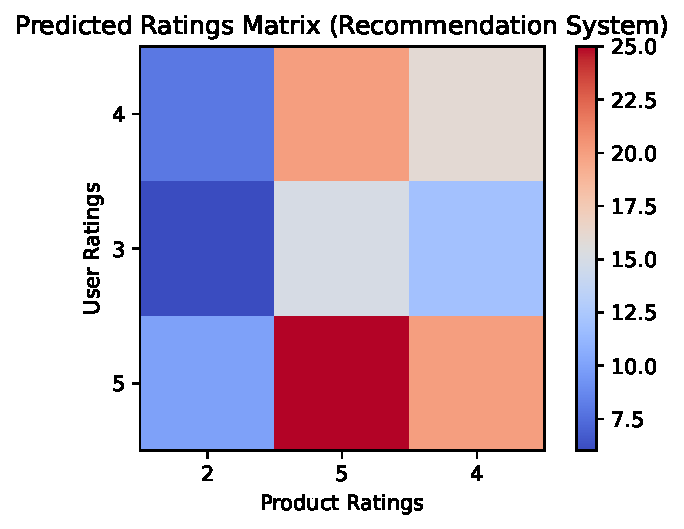
\includegraphics{module_2_files/figure-pdf/cell-29-output-3.pdf}

\begin{tcolorbox}[enhanced jigsaw, rightrule=.15mm, arc=.35mm, breakable, colback=white, toprule=.15mm, colframe=quarto-callout-note-color-frame, toptitle=1mm, opacityback=0, colbacktitle=quarto-callout-note-color!10!white, opacitybacktitle=0.6, title=\textcolor{quarto-callout-note-color}{\faInfo}\hspace{0.5em}{Additional Properties \& Definitions}, bottomrule=.15mm, left=2mm, titlerule=0mm, coltitle=black, bottomtitle=1mm, leftrule=.75mm]

\begin{enumerate}
\def\labelenumi{\arabic{enumi}.}
\item
  \textbf{Definition and Properties}

  Given two vectors:

  \begin{itemize}
  \tightlist
  \item
    \(\mathbf{u} \in \mathbb{R}^m\)
  \item
    \(\mathbf{v} \in \mathbb{R}^n\)
  \end{itemize}

  The outer product \(\mathbf{u} \otimes \mathbf{v}\) results in an
  \(m \times n\) matrix where each element \((i, j)\) of the matrix is
  calculated as:
  \[(\mathbf{u} \otimes \mathbf{v})_{ij} = u_i \cdot v_j\]
\item
  \textbf{Non-Symmetry}

  The outer product is generally not symmetric. For vectors
  \(\mathbf{u}\) and \(\mathbf{v}\), the matrix
  \(\mathbf{u} \otimes \mathbf{v}\) is not necessarily equal to
  \(\mathbf{v} \otimes \mathbf{u}\):
  \[\mathbf{u} \otimes \mathbf{v} \neq \mathbf{v} \otimes \mathbf{u}\]
\item
  \textbf{Rank of the Outer Product}

  The rank of the outer product matrix \(\mathbf{u} \otimes \mathbf{v}\)
  is always 1, provided neither \(\mathbf{u}\) nor \(\mathbf{v}\) is a
  zero vector. This is because the matrix can be expressed as a single
  rank-1 matrix.
\item
  \textbf{Distributive Property}

  The outer product is distributive over vector addition. For vectors
  \(\mathbf{u}_1, \mathbf{u}_2 \in \mathbb{R}^m\) and
  \(\mathbf{v} \in \mathbb{R}^n\):
  \[(\mathbf{u}_1 + \mathbf{u}_2) \otimes \mathbf{v} = (\mathbf{u}_1 \otimes \mathbf{v}) + (\mathbf{u}_2 \otimes \mathbf{v})\]
\item
  \textbf{Associativity with Scalar Multiplication}

  The outer product is associative with scalar multiplication. For a
  scalar \(\alpha\) and vectors \(\mathbf{u} \in \mathbb{R}^m\) and
  \(\mathbf{v} \in \mathbb{R}^n\):
  \[\alpha (\mathbf{u} \otimes \mathbf{v}) = (\alpha \mathbf{u}) \otimes \mathbf{v} = \mathbf{u} \otimes (\alpha \mathbf{v})\]
\item
  \textbf{Matrix Trace}

  The trace of the outer product of two vectors is given by:
  \[\text{tr}(\mathbf{u} \otimes \mathbf{v}) = (\mathbf{u}^T \mathbf{v})= (\mathbf{v}^T \mathbf{u})\]
  Here, \(\text{tr}\) denotes the trace of a matrix, which is the sum of
  its diagonal elements.
\item
  \textbf{Matrix Norm}

  The Frobenius norm of the outer product matrix can be expressed in
  terms of the norms of the original vectors:
  \[\| \mathbf{u} \otimes \mathbf{v} \|_F = \| \mathbf{u} \|_2 \cdot \| \mathbf{v} \|_2\]
  where \(\| \cdot \|_2\) denotes the Euclidean norm.
\end{enumerate}

\end{tcolorbox}

\textbf{Example Calculation in \texttt{Python}}

Here's how to compute and visualize the outer product properties using
\texttt{Python}:

\begin{Shaded}
\begin{Highlighting}[]
\ImportTok{import}\NormalTok{ numpy }\ImportTok{as}\NormalTok{ np}
\ImportTok{import}\NormalTok{ matplotlib.pyplot }\ImportTok{as}\NormalTok{ plt}

\CommentTok{\# Define vectors}
\NormalTok{u }\OperatorTok{=}\NormalTok{ np.array([}\DecValTok{1}\NormalTok{, }\DecValTok{2}\NormalTok{, }\DecValTok{3}\NormalTok{])}
\NormalTok{v }\OperatorTok{=}\NormalTok{ np.array([}\DecValTok{4}\NormalTok{, }\DecValTok{5}\NormalTok{])}

\CommentTok{\# Compute outer product}
\NormalTok{outer\_product }\OperatorTok{=}\NormalTok{ np.outer(u, v)}

\CommentTok{\# Display results}
\BuiltInTok{print}\NormalTok{(}\StringTok{"Outer Product Matrix:"}\NormalTok{)}
\BuiltInTok{print}\NormalTok{(outer\_product)}

\CommentTok{\# Compute and display rank}
\NormalTok{rank }\OperatorTok{=}\NormalTok{ np.linalg.matrix\_rank(outer\_product)}
\BuiltInTok{print}\NormalTok{(}\SpecialStringTok{f"Rank of Outer Product Matrix: }\SpecialCharTok{\{}\NormalTok{rank}\SpecialCharTok{\}}\SpecialStringTok{"}\NormalTok{)}

\CommentTok{\# Compute Frobenius norm}
\NormalTok{frobenius\_norm }\OperatorTok{=}\NormalTok{ np.linalg.norm(outer\_product, }\StringTok{\textquotesingle{}fro\textquotesingle{}}\NormalTok{)}
\BuiltInTok{print}\NormalTok{(}\SpecialStringTok{f"Frobenius Norm: }\SpecialCharTok{\{}\NormalTok{frobenius\_norm}\SpecialCharTok{\}}\SpecialStringTok{"}\NormalTok{)}

\CommentTok{\# Plot the result}
\NormalTok{plt.imshow(outer\_product, cmap}\OperatorTok{=}\StringTok{\textquotesingle{}viridis\textquotesingle{}}\NormalTok{, interpolation}\OperatorTok{=}\StringTok{\textquotesingle{}nearest\textquotesingle{}}\NormalTok{)}
\NormalTok{plt.colorbar()}
\NormalTok{plt.title(}\StringTok{\textquotesingle{}Outer Product Matrix\textquotesingle{}}\NormalTok{)}
\NormalTok{plt.xlabel(}\StringTok{\textquotesingle{}Vector v\textquotesingle{}}\NormalTok{)}
\NormalTok{plt.ylabel(}\StringTok{\textquotesingle{}Vector u\textquotesingle{}}\NormalTok{)}
\NormalTok{plt.xticks(ticks}\OperatorTok{=}\NormalTok{np.arange(}\BuiltInTok{len}\NormalTok{(v)), labels}\OperatorTok{=}\NormalTok{v)}
\NormalTok{plt.yticks(ticks}\OperatorTok{=}\NormalTok{np.arange(}\BuiltInTok{len}\NormalTok{(u)), labels}\OperatorTok{=}\NormalTok{u)}
\NormalTok{plt.show()}
\end{Highlighting}
\end{Shaded}

\begin{verbatim}
Outer Product Matrix:
[[ 4  5]
 [ 8 10]
 [12 15]]
Rank of Outer Product Matrix: 1
Frobenius Norm: 23.958297101421877
\end{verbatim}

\begin{figure}[H]

\centering{

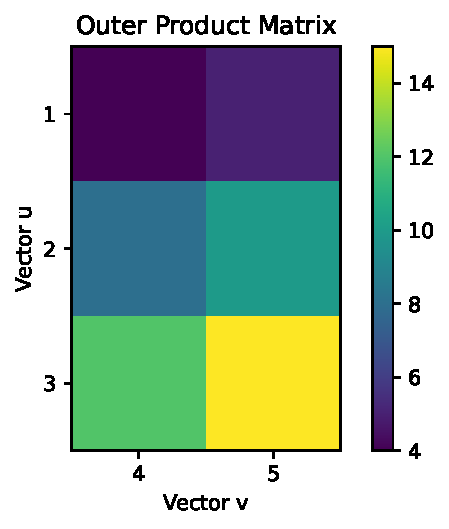
\includegraphics{module_2_files/figure-pdf/fig-op-output-2.pdf}

}

\caption{\label{fig-op}Demonstration of Outer Product and its
Properties}

\end{figure}%

\subsubsection{Kronecker Product}\label{kronecker-product}

In mathematics, the Kronecker product, sometimes denoted by \(\otimes\),
is an operation on two matrices of arbitrary size resulting in a
\emph{block matrix}. It is a specialization of the tensor product (which
is denoted by the same symbol) from vectors to matrices and gives the
matrix of the tensor product linear map with respect to a standard
choice of basis. The Kronecker product is to be distinguished from the
usual matrix multiplication, which is an entirely different operation.
The Kronecker product is also sometimes called \emph{matrix direct
product}.

\begin{tcolorbox}[enhanced jigsaw, rightrule=.15mm, arc=.35mm, breakable, colback=white, toprule=.15mm, colframe=quarto-callout-note-color-frame, toptitle=1mm, opacityback=0, colbacktitle=quarto-callout-note-color!10!white, opacitybacktitle=0.6, title=\textcolor{quarto-callout-note-color}{\faInfo}\hspace{0.5em}{Note}, bottomrule=.15mm, left=2mm, titlerule=0mm, coltitle=black, bottomtitle=1mm, leftrule=.75mm]

If \(A\) is an \(m \times n\) matrix and \(B\) is a \(p \times q\)
matrix, then the Kronecker product \(A\otimes B\) is the
\(pm \times qn\) block matrix defined as: Each \(a_{ij}\) of \(A\) is
replaced by the matrix \(a_{ij}B\). Symbolically this will result in a
block matrix defined by:

\[A\otimes B=\begin{bmatrix}A \otimes B = \begin{bmatrix}a_{11}B & a_{12}B & \cdots & a_{1n}B \\a_{21}B & a_{22}B & \cdots & a_{2n}B \\\vdots & \vdots & \ddots & vdots \\a_{m1}B & a_{m2}B & \cdots & a_{mn}B\end{bmatrix} \end{bmatrix}\]

\end{tcolorbox}

\begin{tcolorbox}[enhanced jigsaw, rightrule=.15mm, arc=.35mm, breakable, colback=white, toprule=.15mm, colframe=quarto-callout-note-color-frame, toptitle=1mm, opacityback=0, colbacktitle=quarto-callout-note-color!10!white, opacitybacktitle=0.6, title=\textcolor{quarto-callout-note-color}{\faInfo}\hspace{0.5em}{Properties of the Kronecker Product}, bottomrule=.15mm, left=2mm, titlerule=0mm, coltitle=black, bottomtitle=1mm, leftrule=.75mm]

\begin{enumerate}
\def\labelenumi{\arabic{enumi}.}
\item
  \textbf{Associativity}

  The Kronecker product is associative. For matrices
  \(A \in \mathbb{R}^{m \times n}\), \(B \in \mathbb{R}^{p \times q}\),
  and \(C \in \mathbb{R}^{r \times s}\):
  \[(A \otimes B) \otimes C = A \otimes (B \otimes C)\]
\item
  \textbf{Distributivity Over Addition}

  The Kronecker product distributes over matrix addition. For matrices
  \(A \in \mathbb{R}^{m \times n}\), \(B \in \mathbb{R}^{p \times q}\),
  and \(C \in \mathbb{R}^{p \times q}\):
  \[A \otimes (B + C) = (A \otimes B) + (A \otimes C)\]
\item
  \textbf{Mixed Product Property}

  The Kronecker product satisfies the mixed product property with the
  matrix product. For matrices \(A \in \mathbb{R}^{m \times n}\),
  \(B \in \mathbb{R}^{p \times q}\), \(C \in \mathbb{R}^{r \times s}\),
  and \(D \in \mathbb{R}^{r \times s}\):
  \[(A \otimes B) (C \otimes D) = (A C) \otimes (B D)\]
\item
  \textbf{Transpose}

  The transpose of the Kronecker product is given by:
  \[(A \otimes B)^T = A^T \otimes B^T\]
\item
  \textbf{Norm}

  The Frobenius norm of the Kronecker product can be computed as:
  \[\| A \otimes B \|_F = \| A \|_F \cdot \| B \|_F\] where
  \(\| \cdot \|_F\) denotes the Frobenius norm.
\end{enumerate}

\end{tcolorbox}

\begin{center}\rule{0.5\linewidth}{0.5pt}\end{center}

\begin{tcolorbox}[enhanced jigsaw, rightrule=.15mm, arc=.35mm, breakable, colback=white, toprule=.15mm, colframe=quarto-callout-tip-color-frame, toptitle=1mm, opacityback=0, colbacktitle=quarto-callout-tip-color!10!white, opacitybacktitle=0.6, title=\textcolor{quarto-callout-tip-color}{\faLightbulb}\hspace{0.5em}{Frobenius Norm}, bottomrule=.15mm, left=2mm, titlerule=0mm, coltitle=black, bottomtitle=1mm, leftrule=.75mm]

The Frobenius norm, also known as the Euclidean norm for matrices, is a
measure of a matrix's magnitude. It is defined as the square root of the
sum of the absolute squares of its elements. Mathematically, for a
matrix \(A\) with elements \(a_{ij}\), the Frobenius norm is given by:

\[\|A\|_F = \sqrt{\sum_{i,j} |a_{ij}|^2}\]

\end{tcolorbox}

Example 1: Calculation of Frobenius Norm

Consider the matrix \(A\):

\[A = \begin{bmatrix}1 & 2 \\3 & 4\end{bmatrix}\]

To compute the Frobenius norm:

\[\|A\|_F = \sqrt{1^2 + 2^2 + 3^2 + 4^2}= \sqrt{1 + 4 + 9 + 16}= \sqrt{30}\approx 5.48\]

Example 2: Frobenius Norm of a Sparse Matrix

Consider the sparse matrix \(B\):

\[B = \begin{bmatrix}0 & 0 & 0 \\0 & 5 & 0 \\0 & 0 & 0\end{bmatrix}\]

To compute the Frobenius norm:

\[\|B\|_F = \sqrt{0^2 + 0^2 + 0^2 + 5^2 + 0^2 + 0^2}= \sqrt{25}= 5\]

Example 3: Frobenius Norm in a Large Matrix

Consider the matrix \(C\) of size \$3 \times 3 \$:

\[C = \begin{bmatrix}1 & 2 & 3 \\4 & 5 & 6 \\7 & 8 & 9\end{bmatrix}\]

To compute the Frobenius norm:

\begin{align*}
\|C\|_F &= \sqrt{1^2 + 2^2 + 3^2 + 4^2 + 5^2 + 6^2 + 7^2 + 8^2 + 9^2}\\
&= \sqrt{1 + 4 + 9 + 16 + 25 + 36 + 49 + 64 + 81}
&= \sqrt{285}
&\approx 16.88
\end{align*}

\textbf{Applications of the Frobenius Norm}

\begin{itemize}
\item
  \emph{Application 1: Image Compression:} In image processing, the
  Frobenius norm can measure the difference between the original and
  compressed images, indicating how well the compression has preserved
  the original image quality.
\item
  \emph{Application 2: Matrix Factorization:} In numerical analysis,
  Frobenius norm is used to evaluate the error in matrix approximations,
  such as in Singular Value Decomposition (SVD). A lower Frobenius norm
  of the error indicates a better approximation.
\item
  \emph{Application 3: Error Measurement in Numerical Solutions:} In
  solving systems of linear equations, the Frobenius norm can be used to
  measure the error between the true solution and the computed solution,
  providing insight into the accuracy of numerical methods.
\end{itemize}

The \texttt{linalg} sub module of \texttt{NumPy} library can be used to
calculate various norms. Basically norm is the generalized form of
Euclidean distance.

\begin{Shaded}
\begin{Highlighting}[]
\ImportTok{import}\NormalTok{ numpy }\ImportTok{as}\NormalTok{ np}

\CommentTok{\# Example 1: Simple Matrix}
\NormalTok{A }\OperatorTok{=}\NormalTok{ np.array([[}\DecValTok{1}\NormalTok{, }\DecValTok{2}\NormalTok{], [}\DecValTok{3}\NormalTok{, }\DecValTok{4}\NormalTok{]])}
\NormalTok{frobenius\_norm\_A }\OperatorTok{=}\NormalTok{ np.linalg.norm(A, }\StringTok{\textquotesingle{}fro\textquotesingle{}}\NormalTok{)}
\BuiltInTok{print}\NormalTok{(}\SpecialStringTok{f"Frobenius Norm of A: }\SpecialCharTok{\{}\NormalTok{frobenius\_norm\_A}\SpecialCharTok{:.2f\}}\SpecialStringTok{"}\NormalTok{)}

\CommentTok{\# Example 2: Sparse Matrix}
\NormalTok{B }\OperatorTok{=}\NormalTok{ np.array([[}\DecValTok{0}\NormalTok{, }\DecValTok{0}\NormalTok{, }\DecValTok{0}\NormalTok{], [}\DecValTok{0}\NormalTok{, }\DecValTok{5}\NormalTok{, }\DecValTok{0}\NormalTok{], [}\DecValTok{0}\NormalTok{, }\DecValTok{0}\NormalTok{, }\DecValTok{0}\NormalTok{]])}
\NormalTok{frobenius\_norm\_B }\OperatorTok{=}\NormalTok{ np.linalg.norm(B, }\StringTok{\textquotesingle{}fro\textquotesingle{}}\NormalTok{)}
\BuiltInTok{print}\NormalTok{(}\SpecialStringTok{f"Frobenius Norm of B: }\SpecialCharTok{\{}\NormalTok{frobenius\_norm\_B}\SpecialCharTok{:.2f\}}\SpecialStringTok{"}\NormalTok{)}

\CommentTok{\# Example 3: Large Matrix}
\NormalTok{C }\OperatorTok{=}\NormalTok{ np.array([[}\DecValTok{1}\NormalTok{, }\DecValTok{2}\NormalTok{, }\DecValTok{3}\NormalTok{], [}\DecValTok{4}\NormalTok{, }\DecValTok{5}\NormalTok{, }\DecValTok{6}\NormalTok{], [}\DecValTok{7}\NormalTok{, }\DecValTok{8}\NormalTok{, }\DecValTok{9}\NormalTok{]])}
\NormalTok{frobenius\_norm\_C }\OperatorTok{=}\NormalTok{ np.linalg.norm(C, }\StringTok{\textquotesingle{}fro\textquotesingle{}}\NormalTok{)}
\BuiltInTok{print}\NormalTok{(}\SpecialStringTok{f"Frobenius Norm of C: }\SpecialCharTok{\{}\NormalTok{frobenius\_norm\_C}\SpecialCharTok{:.2f\}}\SpecialStringTok{"}\NormalTok{)}
\end{Highlighting}
\end{Shaded}

\begin{verbatim}
Frobenius Norm of A: 5.48
Frobenius Norm of B: 5.00
Frobenius Norm of C: 16.88
\end{verbatim}

\textbf{Frobenius norm of Kronecker product}

Let us consider two matrices,

\[A = \begin{bmatrix}1 & 2 \\3 & 4\end{bmatrix}\]

and

\[B = \begin{bmatrix}0 & 5 \\6 & 7\end{bmatrix}\]

The Kronecker product \(C = A \otimes B\) is:

\[C = \begin{bmatrix}1 \cdot B & 2 \cdot B \\3 \cdot B & 4 \cdot B\end{bmatrix}= \begin{bmatrix}\begin{bmatrix}0 & 5 \\6 & 7\end{bmatrix} & \begin{bmatrix}0 \cdot 2 & 5 \cdot 2 \\6 \cdot 2 & 7 \cdot 2\end{bmatrix} \\\begin{bmatrix}0 \cdot 3 & 5 \cdot 3 \\6 \cdot 3 & 7 \cdot 3\end{bmatrix} & \begin{bmatrix}0 \cdot 4 & 5 \cdot 4 \\6 \cdot 4 & 7 \cdot 4\end{bmatrix}\end{bmatrix}\]

This expands to:

\[C = \begin{bmatrix}0 & 5 & 0 & 10 \\6 & 7 & 12 & 14 \\0 & 15 & 0 & 20 \\18 & 21 & 24 & 28\end{bmatrix}\]

\emph{Computing the Frobenius Norm}

To compute the Frobenius norm of \(C\):

\[\|C\|_F = \sqrt{\sum_{i=1}^{4} \sum_{j=1}^{4} |c_{ij}|^2}\]

\[\|C\|_F = \sqrt{0^2 + 5^2 + 0^2 + 10^2 + 6^2 + 7^2 + 12^2 + 14^2 + 0^2 + 15^2 + 0^2 + 20^2 + 18^2 + 21^2 + 24^2 + 28^2}\]

\[\|C\|_F = \sqrt{0 + 25 + 0 + 100 + 36 + 49 + 144 + 196 + 0 + 225 + 0 + 400 + 324 + 441 + 576 + 784}\]

\[\|C\|_F = \sqrt{2896}\] \[\|C\|_F \approx 53.87\]

\begin{center}\rule{0.5\linewidth}{0.5pt}\end{center}

\subsubsection{Practice Problems}\label{practice-problems-4}

\textbf{Find the Kronecker product of A and B where A and B are given as
follows:}

\textbf{Problem 1:}

Find the Kronecker product of:
\[A=\begin{bmatrix}1&2\\3&4\end{bmatrix}\]
\[B=\begin{bmatrix}0&1\\1&0\end{bmatrix}\]

\textbf{Solution:}

\begin{align*}
A \otimes B &= \begin{bmatrix}1&2\\3&4\end{bmatrix} \otimes \begin{bmatrix}0&1\\1&0\end{bmatrix} \\
&= \begin{bmatrix}
1 \cdot \begin{bmatrix}0&1\\1&0\end{bmatrix} & 2 \cdot \begin{bmatrix}0&1\\1&0\end{bmatrix} \\
3 \cdot \begin{bmatrix}0&1\\1&0\end{bmatrix} & 4 \cdot \begin{bmatrix}0&1\\1&0\end{bmatrix}
\end{bmatrix} \\
&= \begin{bmatrix}
0 & 1 & 0 & 2 \\
1 & 0 & 2& 0\\
0 & 3 & 0 & 4 \\
3 & 0 & 4 & 0
\end{bmatrix}
\end{align*}

\begin{center}\rule{0.5\linewidth}{0.5pt}\end{center}

\textbf{Problem 2:}

Find the Kronecker product of:
\[A=\begin{bmatrix}1&0\\0&1\end{bmatrix}\]
\[B=\begin{bmatrix}2&3\\4&5\end{bmatrix}\]

\textbf{Solution:}

\begin{align*}
A \otimes B &= \begin{bmatrix}1&0\\0&1\end{bmatrix} \otimes \begin{bmatrix}2&3\\4&5\end{bmatrix} \\
&= \begin{bmatrix}
1 \cdot \begin{bmatrix}2&3\\4&5\end{bmatrix} & 0 \cdot \begin{bmatrix}2&3\\4&5\end{bmatrix} \\
0 \cdot \begin{bmatrix}2&3\\4&5\end{bmatrix} & 1 \cdot \begin{bmatrix}2&3\\4&5\end{bmatrix}
\end{bmatrix} \\
&= \begin{bmatrix}
2 & 3 & 0 & 0 \\
4 & 5 & 0 & 0 \\
0 & 0 & 2 & 3 \\
0 & 0 & 4 & 5
\end{bmatrix}
\end{align*}

\begin{center}\rule{0.5\linewidth}{0.5pt}\end{center}

\textbf{Problem 3:}

Find the Kronecker product of: \[A=\begin{bmatrix}1&2\end{bmatrix}\]
\[B=\begin{bmatrix}3\\4\end{bmatrix}\]

\textbf{Solution:}

\begin{align*}
A \otimes B &= \begin{bmatrix}1&2\end{bmatrix} \otimes \begin{bmatrix}3\\4\end{bmatrix} \\
&= \begin{bmatrix}
1 \cdot \begin{bmatrix}3\\4\end{bmatrix} & 2 \cdot \begin{bmatrix}3\\4\end{bmatrix}
\end{bmatrix} \\
&= \begin{bmatrix}
3 & 6 \\
4 & 8
\end{bmatrix}
\end{align*}

\begin{center}\rule{0.5\linewidth}{0.5pt}\end{center}

\textbf{Problem 4:}

Find the Kronecker product of: \[A=\begin{bmatrix}0&1\end{bmatrix}\]
\[B=\begin{bmatrix}1&-1\\2&0\end{bmatrix}\]

\textbf{Solution:}

\begin{align*}
A \otimes B &= \begin{bmatrix}0&1\end{bmatrix} \otimes \begin{bmatrix}1&-1\\2&0\end{bmatrix} \\
&= \begin{bmatrix}
0 \cdot \begin{bmatrix}1&-1\\2&0\end{bmatrix} & 1 \cdot \begin{bmatrix}1&-1\\2&0\end{bmatrix}
\end{bmatrix} \\
&= \begin{bmatrix}
0 & 0 &1&-1\\
0 & 0&2&0 \\
\end{bmatrix}
\end{align*}

\begin{center}\rule{0.5\linewidth}{0.5pt}\end{center}

\textbf{Problem 5:}

Find the Kronecker product of: \[A=\begin{bmatrix}2\\3\end{bmatrix}\]
\[B=\begin{bmatrix}4&-2\end{bmatrix}\]

\textbf{Solution:}

\begin{align*}
A \otimes B &= \begin{bmatrix}2\\3\end{bmatrix} \otimes \begin{bmatrix}4&-2\end{bmatrix} \\
&= \begin{bmatrix}
2 \cdot \begin{bmatrix}4&-2\end{bmatrix} \\
3 \cdot \begin{bmatrix}4&-2\end{bmatrix}
\end{bmatrix} \\
&= \begin{bmatrix}
8 & -4 \\
12 & -6
\end{bmatrix}
\end{align*}

\begin{center}\rule{0.5\linewidth}{0.5pt}\end{center}

\textbf{Problem 6:}

Find the Kronecker product of:
\[A=\begin{bmatrix}1&-1\\0&2\end{bmatrix}\]
\[B=\begin{bmatrix}0&1\\1&0\end{bmatrix}\]

\textbf{Solution:}

\begin{align*}
A \otimes B &= \begin{bmatrix}1&-1\\0&2\end{bmatrix} \otimes \begin{bmatrix}0&1\\1&0\end{bmatrix} \\
&= \begin{bmatrix}
1 \cdot \begin{bmatrix}0&1\\1&0\end{bmatrix} & -1 \cdot \begin{bmatrix}0&1\\1&0\end{bmatrix} \\
0 \cdot \begin{bmatrix}0&1\\1&0\end{bmatrix} & 2 \cdot \begin{bmatrix}0&1\\1&0\end{bmatrix}
\end{bmatrix} \\
&= \begin{bmatrix}
0 & 1 & 0 & -1 \\
1 & 0 & -1 & 0 \\
0 & 0 & 0 & 2 \\
0 & 0 & 2 & 0
\end{bmatrix}
\end{align*}

\begin{center}\rule{0.5\linewidth}{0.5pt}\end{center}

\textbf{Problem 7:}

Find the Kronecker product of: \[A=\begin{bmatrix}2\end{bmatrix}\]
\[B=\begin{bmatrix}3&4\\5&6\end{bmatrix}\]

\textbf{Solution:}

\begin{align*}
A \otimes B &= \begin{bmatrix}2\end{bmatrix} \otimes \begin{bmatrix}3&4\\5&6\end{bmatrix} \\
&= 2 \cdot \begin{bmatrix}3&4\\5&6\end{bmatrix} \\
&= \begin{bmatrix}
6 & 8 \\
10 & 12
\end{bmatrix}
\end{align*}

\begin{center}\rule{0.5\linewidth}{0.5pt}\end{center}

\textbf{Problem 8:}

Find the Kronecker product of: \[A=\begin{bmatrix}0&1\end{bmatrix}\]
\[B=\begin{bmatrix}1&0\\0&1\end{bmatrix}\]

\textbf{Solution:}

\begin{align*}
A \otimes B &= \begin{bmatrix}0&1\end{bmatrix} \otimes \begin{bmatrix}1&0\\0&1\end{bmatrix} \\
&= \begin{bmatrix}
0 \cdot \begin{bmatrix}1&0\\0&1\end{bmatrix} & 1 \cdot \begin{bmatrix}1&0\\0&1\end{bmatrix}
\end{bmatrix} \\
&= \begin{bmatrix}
0 & 0 \\
0 & 1
\end{bmatrix}
\end{align*}

\begin{center}\rule{0.5\linewidth}{0.5pt}\end{center}

\textbf{Problem 9:}

Find the Kronecker product of:
\[A=\begin{bmatrix}1&0\\0&1\end{bmatrix}\]
\[B=\begin{bmatrix}1&1\\1&1\end{bmatrix}\]

\textbf{Solution:}

\begin{align*}
A \otimes B &= \begin{bmatrix}1&0\\0&1\end{bmatrix} \otimes \begin{bmatrix}1&1\\1&1\end{bmatrix} \\
&= \begin{bmatrix}
1 \cdot \begin{bmatrix}1&1\\1&1\end{bmatrix} & 0 \cdot \begin{bmatrix}1&1\\1&1\end{bmatrix} \\
0 \cdot \begin{bmatrix}1&1\\1&1\end{bmatrix} & 1 \cdot \begin{bmatrix}1&1\\1&1\end{bmatrix}
\end{bmatrix} \\
&= \begin{bmatrix}
1 & 1 & 0 & 0 \\
1 & 1 & 0 & 0 \\
0 & 0 & 1 & 1 \\
0 & 0 & 1 & 1
\end{bmatrix}
\end{align*}

\begin{center}\rule{0.5\linewidth}{0.5pt}\end{center}

\textbf{Problem 10:}

Find the Kronecker product of:
\[A=\begin{bmatrix}2&-1\\3&4\end{bmatrix}\]
\[B=\begin{bmatrix}0&5\\-2&3\end{bmatrix}\]

\textbf{Solution:}

\begin{align*}
A \otimes B &= \begin{bmatrix}2&-1\\3&4\end{bmatrix} \otimes \begin{bmatrix}0&5\\-2&3\end{bmatrix} \\
&= \begin{bmatrix}
2 \cdot \begin{bmatrix}0&5\\-2&3\end{bmatrix} & -1 \cdot \begin{bmatrix}0&5\\-2&3\end{bmatrix} \\
3 \cdot \begin{bmatrix}0&5\\-2&3\end{bmatrix} & 4 \cdot \begin{bmatrix}0&5\\-2&3\end{bmatrix}
\end{bmatrix} \\
&= \begin{bmatrix}
0 & 10 & 0 & -5 \\
-4 & 6 & 2 & -3 \\
0 & 15 & 0 & 20 \\
-6 & 9 & -8 & 12
\end{bmatrix}
\end{align*}

\begin{center}\rule{0.5\linewidth}{0.5pt}\end{center}

\subsubsection{Connection Between Outer Product and Kronecker
Product}\label{connection-between-outer-product-and-kronecker-product}

\begin{enumerate}
\def\labelenumi{\arabic{enumi}.}
\item
  \textbf{Conceptual Connection:}

  \begin{itemize}
  \item
    The \textbf{outer product} is a special case of the
    \textbf{Kronecker product}. Specifically, if \(\mathbf{A}\) is a
    column vector and \(\mathbf{B}\) is a row vector, then
    \(\mathbf{A}\) is a \(m \times 1\) matrix and \(\mathbf{B}\) is a
    \(1 \times n\) matrix. The Kronecker product of these two matrices
    will yield the same result as the outer product of these vectors.
  \item
    For matrices \(\mathbf{A}\) and \(\mathbf{B}\), the Kronecker
    product involves taking the outer product of each element of
    \(\mathbf{A}\) with the entire matrix \(\mathbf{B}\).
  \end{itemize}
\item
  \textbf{Mathematical Formulation:}

  \begin{itemize}
  \tightlist
  \item
    Let
    \(\mathbf{A} = \begin{bmatrix}a_{11} & a_{12}\\ a_{21} & a_{22}\end{bmatrix}\)
    and
    \(\mathbf{B} = \begin{bmatrix}b_{11} & b_{12}\\ b_{21} & b_{22}\end{bmatrix}\).
    Then:
  \end{itemize}

  \[\mathbf{A} \otimes \mathbf{B} = \begin{bmatrix} a_{11} \mathbf{B} & a_{12} \mathbf{B} \\ a_{21} \mathbf{B} & a_{22} \mathbf{B} \end{bmatrix}\]

  \begin{itemize}
  \tightlist
  \item
    If \(\mathbf{A} = \mathbf{u} \mathbf{v}^T\) where \(\mathbf{u}\) is
    a column vector and \(\mathbf{v}^T\) is a row vector, then the
    Kronecker product of \(\mathbf{u}\) and \(\mathbf{v}^T\) yields the
    same result as the outer product \(\mathbf{u} \otimes \mathbf{v}\).
  \end{itemize}
\end{enumerate}

\begin{tcolorbox}[enhanced jigsaw, rightrule=.15mm, arc=.35mm, breakable, colback=white, toprule=.15mm, colframe=quarto-callout-note-color-frame, toptitle=1mm, opacityback=0, colbacktitle=quarto-callout-note-color!10!white, opacitybacktitle=0.6, title=\textcolor{quarto-callout-note-color}{\faInfo}\hspace{0.5em}{Note}, bottomrule=.15mm, left=2mm, titlerule=0mm, coltitle=black, bottomtitle=1mm, leftrule=.75mm]

\textbf{Summary}

\begin{itemize}
\tightlist
\item
  The \textbf{outer product} is a specific case of the \textbf{Kronecker
  product} where one of the matrices is a vector (either row or column).
\item
  The \textbf{Kronecker product} generalizes the outer product to
  matrices and is more versatile in applications involving tensor
  products and higher-dimensional constructs.
\end{itemize}

\end{tcolorbox}

\subsubsection{Matrix Multiplication as Kronecker
Product}\label{matrix-multiplication-as-kronecker-product}

Given matrices \(\mathbf{A}\) and \(\mathbf{B}\), where: -
\(\mathbf{A}\) is an \(m \times n\) matrix - \(\mathbf{B}\) is an
\(n \times p\) matrix

The product \(\mathbf{C} = \mathbf{A} \mathbf{B}\) can be expressed
using Kronecker products as:

\[\mathbf{C} = \sum_{k=1}^n (\mathbf{A}_{:,k} \otimes \mathbf{B}_{k,:})\]

where: - \(\mathbf{A}_{:,k}\) denotes the \(k\)-th column of matrix
\(\mathbf{A}\) - \(\mathbf{B}_{k,:}\) denotes the \(k\)-th row of matrix
\(\mathbf{B}\)

\textbf{Example:}

Let:

\[\mathbf{A} = \begin{bmatrix}1 & 2 \\3 & 4\end{bmatrix}\]

and:

\[\mathbf{B} = \begin{bmatrix}0 & 1 \\1 & 0\end{bmatrix}\]

To find \(\mathbf{C} = \mathbf{A} \mathbf{B}\) using Kronecker products:

\begin{enumerate}
\def\labelenumi{\arabic{enumi}.}
\item
  \textbf{Compute the Kronecker Product of Columns of \(\mathbf{A}\) and
  Rows of \(\mathbf{B}\):}

  \begin{itemize}
  \item
    For column
    \(\mathbf{A}_{:,1} = \begin{bmatrix} 1 \\ 3 \end{bmatrix}\) and row
    \(\mathbf{B}_{1,:} = \begin{bmatrix} 0 & 1 \end{bmatrix}\):
    \[\mathbf{A}_{:,1} \otimes \mathbf{B}_{1,:} = \begin{bmatrix}     0 & 1 \\     0 & 3     \end{bmatrix}\]
  \item
    For column
    \(\mathbf{A}_{:,2} = \begin{bmatrix} 2 \\ 4 \end{bmatrix}\) and row
    \(\mathbf{B}_{2,:} = \begin{bmatrix} 1 & 0 \end{bmatrix}\):
    \[\mathbf{A}_{:,2} \otimes \mathbf{B}_{2,:} = \begin{bmatrix}2 & 0 \\ 4 & 0\end{bmatrix}\]
  \end{itemize}
\item
  \textbf{Sum the Kronecker Products:}

  \[\mathbf{C} = \begin{bmatrix}0 & 1 \\ 0 & 3\end{bmatrix} +\begin{bmatrix} 2 & 0 \\ 4 & 0 \end{bmatrix}  = \begin{bmatrix} 2 & 1 \\ 4 & 3\end{bmatrix}\]
\end{enumerate}

\begin{center}\rule{0.5\linewidth}{0.5pt}\end{center}

In the previous block we have discussed the Frobenius norm and its
applications. Now came back to the discussions on the Kronecker product.
The Kronecker product is particularly useful in scenarios where
interactions between different types of data need to be modeled
comprehensively. In recommendation systems, it allows us to integrate
user preferences with item relationships to improve recommendation
accuracy.

In addition to recommendation systems, Kronecker products are used in
various fields such as:

\begin{itemize}
\tightlist
\item
  Signal Processing: For modeling multi-dimensional signals.
\item
  Machine Learning: In building features for complex models.
\item
  Communication Systems: For modeling network interactions.
\end{itemize}

By understanding the Kronecker product and its applications, we can
extend it to solve complex problems and enhance systems across different
domains. To understand the practical use of Kronecker product in a
Machine Learning scenario let us consider the following problem
statement and its solution.

\begin{tcolorbox}[enhanced jigsaw, rightrule=.15mm, arc=.35mm, breakable, colback=white, toprule=.15mm, colframe=quarto-callout-note-color-frame, toptitle=1mm, opacityback=0, colbacktitle=quarto-callout-note-color!10!white, opacitybacktitle=0.6, title=\textcolor{quarto-callout-note-color}{\faInfo}\hspace{0.5em}{Problem statement}, bottomrule=.15mm, left=2mm, titlerule=0mm, coltitle=black, bottomtitle=1mm, leftrule=.75mm]

In the realm of recommendation systems, predicting user preferences for
various product categories based on past interactions is a common
challenge. Suppose we have data on user preferences for different
products and categories. We can use this data to recommend the best
products for each user by employing mathematical tools such as the
Kronecker product. The User Preference and Category relationships are
given in Table~\ref{tbl-UPM} and Table~\ref{tbl-CRM} .

\begin{longtable}[]{@{}llll@{}}
\caption{User Preference}\label{tbl-UPM}\tabularnewline
\toprule\noalign{}
User/Item & Electronics & Clothing & Books \\
\midrule\noalign{}
\endfirsthead
\toprule\noalign{}
User/Item & Electronics & Clothing & Books \\
\midrule\noalign{}
\endhead
\bottomrule\noalign{}
\endlastfoot
User 1 & 5 & 3 & 4 \\
User 2 & 2 & 4 & 5 \\
User 3 & 3 & 4 & 4 \\
\end{longtable}

\begin{longtable}[]{@{}llll@{}}
\caption{Category Relationships}\label{tbl-CRM}\tabularnewline
\toprule\noalign{}
Category/Feature & Feature 1 & Feature 2 & Feature 3 \\
\midrule\noalign{}
\endfirsthead
\toprule\noalign{}
Category/Feature & Feature 1 & Feature 2 & Feature 3 \\
\midrule\noalign{}
\endhead
\bottomrule\noalign{}
\endlastfoot
Electronics & 1 & 0 & 0 \\
Clothing & 0 & 1 & 1 \\
Books & 0 & 1 & 1 \\
\end{longtable}

Predict user preferences for different product categories using the
Kronecker product matrix.

\end{tcolorbox}

\begin{quote}
\textbf{Solution Procedure}
\end{quote}

\begin{enumerate}
\def\labelenumi{\arabic{enumi}.}
\item
  \emph{Compute the Kronecker Product:} Calculate the Kronecker product
  of matrices \(U\) and \(C\) to obtain matrix \(K\).

  To model the problem, we use the Kronecker product of the user
  preference matrix \(U\) and the category relationships matrix \(C\).
  This product allows us to predict the user's rating for each category
  by combining their preferences with the category features.
\end{enumerate}

\emph{Formulating Matrices}

User Preference Matrix (U): - Dimension: \(3\times 3\) (3 users, 3
items) - from the User preference data, we can create the User
Preference Matrix as follows:

\[U = \begin{pmatrix}5 & 3 & 4 \\2 & 4 & 5 \\3 & 4 & 4 \end{pmatrix}\]

Category Relationships Matrix (C): - Dimension: \(3 \times 3\) (3
categories) - from the Category Relationships data, we can create the
Category Relationship Matrix as follows:

\[C = \begin{pmatrix}1 & 0 & 0 \\ 0 & 1 & 1 \\ 0 & 1 & 1\end{pmatrix}\]

\emph{Kronecker Product Calculation}

The Kronecker product \(K\) of \(U\) and \(C\) is calculated as follows:

\begin{enumerate}
\def\labelenumi{\arabic{enumi}.}
\tightlist
\item
  \textbf{Matrix Dimensions:}
\end{enumerate}

\begin{itemize}
\tightlist
\item
  \(U\) is \(3 \times 3\) (3 users, 3 items).
\item
  \(C\) is \(3 \times 3\) (3 categories, 3 features).
\end{itemize}

\begin{enumerate}
\def\labelenumi{\arabic{enumi}.}
\setcounter{enumi}{1}
\tightlist
\item
  \textbf{Calculate Kronecker Product:}
\end{enumerate}

\begin{itemize}
\tightlist
\item
  For each element \(u_{ij}\) in \(U\), multiply by the entire matrix
  \(C\).
\end{itemize}

The Kronecker product \(K\) is computed as:

\[K = U \otimes C\]

Explicitly, the Kronecker product \(K\) is:

\[K = \begin{pmatrix}5 \cdot C & 3 \cdot C & 4 \cdot C \\ 2 \cdot C & 4 \cdot C & 5 \cdot C \\    3 \cdot C & 4 \cdot C & 4 \cdot C\end{pmatrix}\]

As an example the blocks in first row are:

\[5 \cdot C = \begin{pmatrix}   5 & 0 & 0 \\   0 & 5 & 5 \\   0 & 5 & 5   \end{pmatrix}, \quad    3 \cdot C = \begin{pmatrix}   3 & 0 & 0 \\   0 & 3 & 3 \\   0 & 3 & 3   \end{pmatrix}, \quad   4 \cdot C = \begin{pmatrix}   4 & 0 & 0 \\   0 & 4 & 4 \\   0 & 4 & 4   \end{pmatrix}\]

Combining these blocks:

\[K = \begin{pmatrix}   5 & 0 & 0 & 3 & 0 & 0 & 4 & 0 & 0\\   0 & 5 & 5 & 0 & 3 & 3 & 0 & 4 & 4\\   0 & 5 & 5 & 0 & 3 & 3 & 0 & 4 & 4\\   2 & 0 & 0 & 4 & 0 & 0 & 5 & 0 & 0\\   0 & 2 & 2 & 0 & 4 & 4 & 0 & 5 & 5\\   0 & 2 & 2 & 0 & 4 & 4 & 0 & 5 & 5\\   3 & 0 & 0 & 4 & 0 & 0 & 4 & 0 & 0\\   0 & 3 & 3 & 0 & 4 & 4 & 0 & 4 & 4\\   0 & 3 & 3 & 0 & 4 & 4 & 0 & 4 & 4\end{pmatrix}\]

\begin{enumerate}
\def\labelenumi{\arabic{enumi}.}
\setcounter{enumi}{1}
\item
  \textbf{Interpret the Kronecker Product Matrix:} The resulting matrix
  \(K\) represents all possible combinations of user preferences and
  category features.
\item
  \textbf{Predict Ratings:} For each user, use matrix \(K\) to predict
  the rating for each category by summing up the values in the
  corresponding rows.
\item
  \textbf{Generate Recommendations:} Identify the top categories with
  the highest predicted ratings for each user.
\end{enumerate}

The \texttt{python} code to solve this problem computationally is given
below.

\begin{Shaded}
\begin{Highlighting}[]
\ImportTok{import}\NormalTok{ numpy }\ImportTok{as}\NormalTok{ np}
\ImportTok{import}\NormalTok{ pandas }\ImportTok{as}\NormalTok{ pd}
\ImportTok{import}\NormalTok{ matplotlib.pyplot }\ImportTok{as}\NormalTok{ plt}

\CommentTok{\# Define the matrices}
\NormalTok{U }\OperatorTok{=}\NormalTok{ np.array([[}\DecValTok{5}\NormalTok{, }\DecValTok{3}\NormalTok{, }\DecValTok{4}\NormalTok{],}
\NormalTok{              [}\DecValTok{2}\NormalTok{, }\DecValTok{4}\NormalTok{, }\DecValTok{5}\NormalTok{],}
\NormalTok{              [}\DecValTok{3}\NormalTok{, }\DecValTok{4}\NormalTok{, }\DecValTok{4}\NormalTok{]])}

\NormalTok{C }\OperatorTok{=}\NormalTok{ np.array([[}\DecValTok{1}\NormalTok{, }\DecValTok{0}\NormalTok{, }\DecValTok{0}\NormalTok{],}
\NormalTok{              [}\DecValTok{0}\NormalTok{, }\DecValTok{1}\NormalTok{, }\DecValTok{1}\NormalTok{],}
\NormalTok{              [}\DecValTok{0}\NormalTok{, }\DecValTok{1}\NormalTok{, }\DecValTok{1}\NormalTok{]])}

\CommentTok{\# Compute the Kronecker product}
\NormalTok{K }\OperatorTok{=}\NormalTok{ np.kron(U, C)}

\CommentTok{\# Create a DataFrame to visualize the Kronecker product matrix}
\NormalTok{df\_K }\OperatorTok{=}\NormalTok{ pd.DataFrame(K, }
\NormalTok{                    columns}\OperatorTok{=}\NormalTok{[}\StringTok{\textquotesingle{}Electronics\_F1\textquotesingle{}}\NormalTok{, }\StringTok{\textquotesingle{}Electronics\_F2\textquotesingle{}}\NormalTok{, }\StringTok{\textquotesingle{}Electronics\_F3\textquotesingle{}}\NormalTok{, }
                             \StringTok{\textquotesingle{}Clothing\_F1\textquotesingle{}}\NormalTok{, }\StringTok{\textquotesingle{}Clothing\_F2\textquotesingle{}}\NormalTok{, }\StringTok{\textquotesingle{}Clothing\_F3\textquotesingle{}}\NormalTok{, }
                             \StringTok{\textquotesingle{}Books\_F1\textquotesingle{}}\NormalTok{, }\StringTok{\textquotesingle{}Books\_F2\textquotesingle{}}\NormalTok{, }\StringTok{\textquotesingle{}Books\_F3\textquotesingle{}}\NormalTok{],}
\NormalTok{                    index}\OperatorTok{=}\NormalTok{[}\StringTok{\textquotesingle{}User 1 Electronics\textquotesingle{}}\NormalTok{, }\StringTok{\textquotesingle{}User 1 Clothing\textquotesingle{}}\NormalTok{, }\StringTok{\textquotesingle{}User 1 Books\textquotesingle{}}\NormalTok{, }
                           \StringTok{\textquotesingle{}User 2 Electronics\textquotesingle{}}\NormalTok{, }\StringTok{\textquotesingle{}User 2 Clothing\textquotesingle{}}\NormalTok{, }\StringTok{\textquotesingle{}User 2 Books\textquotesingle{}}\NormalTok{, }
                           \StringTok{\textquotesingle{}User 3 Electronics\textquotesingle{}}\NormalTok{, }\StringTok{\textquotesingle{}User 3 Clothing\textquotesingle{}}\NormalTok{, }\StringTok{\textquotesingle{}User 3 Books\textquotesingle{}}\NormalTok{])}

\CommentTok{\# Print the Kronecker product matrix}
\BuiltInTok{print}\NormalTok{(}\StringTok{"Kronecker Product Matrix (K):}\CharTok{\textbackslash{}n}\StringTok{"}\NormalTok{, df\_K)}

\CommentTok{\# Predict ratings and create recommendations}
\KeywordTok{def}\NormalTok{ recommend(user\_index, top\_n}\OperatorTok{=}\DecValTok{3}\NormalTok{):}
    \CommentTok{""" Recommend top\_n categories for a given user based on Kronecker product matrix. """}
\NormalTok{    user\_ratings }\OperatorTok{=}\NormalTok{ K[user\_index }\OperatorTok{*} \BuiltInTok{len}\NormalTok{(C):(user\_index }\OperatorTok{+} \DecValTok{1}\NormalTok{) }\OperatorTok{*} \BuiltInTok{len}\NormalTok{(C), :]}
\NormalTok{    predicted\_ratings }\OperatorTok{=}\NormalTok{ np.}\BuiltInTok{sum}\NormalTok{(user\_ratings, axis}\OperatorTok{=}\DecValTok{0}\NormalTok{)}
\NormalTok{    recommendations }\OperatorTok{=}\NormalTok{ np.argsort(predicted\_ratings)[::}\OperatorTok{{-}}\DecValTok{1}\NormalTok{][:top\_n]}
    \ControlFlowTok{return}\NormalTok{ recommendations}

\CommentTok{\# Recommendations for User 1}
\NormalTok{user\_index }\OperatorTok{=} \DecValTok{0}  \CommentTok{\# User 1}
\NormalTok{top\_n }\OperatorTok{=} \DecValTok{3}
\NormalTok{recommendations }\OperatorTok{=}\NormalTok{ recommend(user\_index, top\_n)}

\BuiltInTok{print}\NormalTok{(}\SpecialStringTok{f"}\CharTok{\textbackslash{}n}\SpecialStringTok{Top }\SpecialCharTok{\{}\NormalTok{top\_n}\SpecialCharTok{\}}\SpecialStringTok{ recommendations for User }\SpecialCharTok{\{}\NormalTok{user\_index }\OperatorTok{+} \DecValTok{1}\SpecialCharTok{\}}\SpecialStringTok{:"}\NormalTok{)}
\ControlFlowTok{for}\NormalTok{ rec }\KeywordTok{in}\NormalTok{ recommendations:}
    \BuiltInTok{print}\NormalTok{(df\_K.columns[rec])}
\end{Highlighting}
\end{Shaded}

\begin{verbatim}
Kronecker Product Matrix (K):
                     Electronics_F1  Electronics_F2  Electronics_F3  \
User 1 Electronics               5               0               0   
User 1 Clothing                  0               5               5   
User 1 Books                     0               5               5   
User 2 Electronics               2               0               0   
User 2 Clothing                  0               2               2   
User 2 Books                     0               2               2   
User 3 Electronics               3               0               0   
User 3 Clothing                  0               3               3   
User 3 Books                     0               3               3   

                    Clothing_F1  Clothing_F2  Clothing_F3  Books_F1  Books_F2  \
User 1 Electronics            3            0            0         4         0   
User 1 Clothing               0            3            3         0         4   
User 1 Books                  0            3            3         0         4   
User 2 Electronics            4            0            0         5         0   
User 2 Clothing               0            4            4         0         5   
User 2 Books                  0            4            4         0         5   
User 3 Electronics            4            0            0         4         0   
User 3 Clothing               0            4            4         0         4   
User 3 Books                  0            4            4         0         4   

                    Books_F3  
User 1 Electronics         0  
User 1 Clothing            4  
User 1 Books               4  
User 2 Electronics         0  
User 2 Clothing            5  
User 2 Books               5  
User 3 Electronics         0  
User 3 Clothing            4  
User 3 Books               4  

Top 3 recommendations for User 1:
Electronics_F2
Electronics_F3
Books_F3
\end{verbatim}

A simple visualization of this recomendation system is shown in
Fig~\ref{fig-reco}.

\begin{Shaded}
\begin{Highlighting}[]
\CommentTok{\# Visualization}
\KeywordTok{def}\NormalTok{ plot\_recommendations(user\_index):}
    \CommentTok{""" Plot the predicted ratings for each category for a given user. """}
\NormalTok{    user\_ratings }\OperatorTok{=}\NormalTok{ K[user\_index }\OperatorTok{*} \BuiltInTok{len}\NormalTok{(C):(user\_index }\OperatorTok{+} \DecValTok{1}\NormalTok{) }\OperatorTok{*} \BuiltInTok{len}\NormalTok{(C), :]}
\NormalTok{    predicted\_ratings }\OperatorTok{=}\NormalTok{ np.}\BuiltInTok{sum}\NormalTok{(user\_ratings, axis}\OperatorTok{=}\DecValTok{0}\NormalTok{)}
\NormalTok{    categories }\OperatorTok{=}\NormalTok{ df\_K.columns}
\NormalTok{    plt.figure(figsize}\OperatorTok{=}\NormalTok{(}\DecValTok{6}\NormalTok{, }\DecValTok{5}\NormalTok{))}
\NormalTok{    plt.bar(categories, predicted\_ratings)}
\NormalTok{    plt.xlabel(}\StringTok{\textquotesingle{}Categories\textquotesingle{}}\NormalTok{)}
\NormalTok{    plt.ylabel(}\StringTok{\textquotesingle{}Predicted Ratings\textquotesingle{}}\NormalTok{)}
\NormalTok{    plt.title(}\SpecialStringTok{f\textquotesingle{}Predicted Ratings for User }\SpecialCharTok{\{}\NormalTok{user\_index }\OperatorTok{+} \DecValTok{1}\SpecialCharTok{\}}\SpecialStringTok{\textquotesingle{}}\NormalTok{)}
\NormalTok{    plt.xticks(rotation}\OperatorTok{=}\DecValTok{45}\NormalTok{)}
\NormalTok{    plt.show()}

\CommentTok{\# Plot recommendations for User 1}
\NormalTok{plot\_recommendations(user\_index)}
\end{Highlighting}
\end{Shaded}

\begin{figure}[H]

\centering{

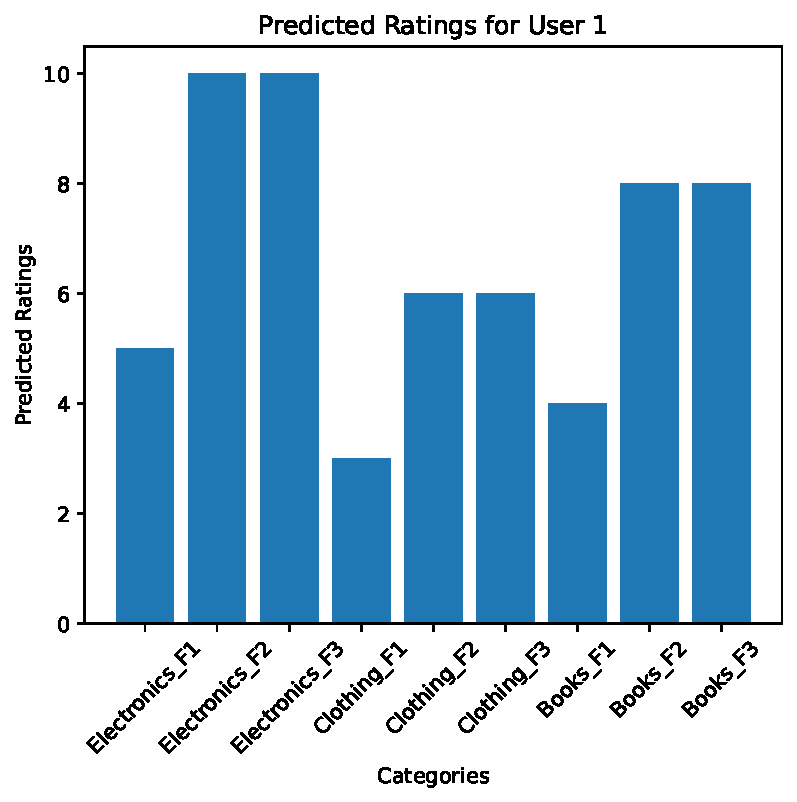
\includegraphics{module_2_files/figure-pdf/fig-reco-output-1.pdf}

}

\caption{\label{fig-reco}EDA for the Recommendation System}

\end{figure}%

This micro project illustrate one of the popular use of Kronecker
product on ML application.

\subsection{Matrix Measures of Practical
Importance}\label{matrix-measures-of-practical-importance}

Matrix measures, such as rank and determinant, play crucial roles in
linear algebra. While both rank and determinant provide valuable
insights into the properties of a matrix, they serve different purposes.
Understanding their roles and applications is essential for solving
complex problems in computer science, engineering, and applied
mathematics.

\subsubsection{Determinant}\label{determinant-1}

Determinant of a \(2\times 2\) matrix
\(A=\begin{pmatrix}a&b\\c&d\end{pmatrix}\) is defined as \(|A|=ad-bc\).
Determinant of higher order square matrices can be found using the
Laplace method or Sarrus method.

The determinant of a matrix provides information about the matrix's
invertibility and scaling factor for volume transformation.
Specifically:

\begin{enumerate}
\def\labelenumi{\arabic{enumi}.}
\item
  \emph{Invertibility:} A matrix is invertible if and only if its
  determinant is non-zero.
\item
  \emph{Volume Scaling:} The absolute value of the determinant gives the
  scaling factor by which the matrix transforms volume.
\item
  \emph{Parallelism:} If the determinant of a matrix composed of vectors
  is zero, the vectors are linearly dependent, meaning they are parallel
  or redundant.
\item
  \emph{Redundancy:} A zero determinant indicates that the vectors span
  a space of lower dimension than the number of vectors, showing
  redundancy.
\end{enumerate}

\begin{tcolorbox}[enhanced jigsaw, rightrule=.15mm, arc=.35mm, breakable, colback=white, toprule=.15mm, colframe=quarto-callout-important-color-frame, toptitle=1mm, opacityback=0, colbacktitle=quarto-callout-important-color!10!white, opacitybacktitle=0.6, title=\textcolor{quarto-callout-important-color}{\faExclamation}\hspace{0.5em}{Least Possible Values of Determinant}, bottomrule=.15mm, left=2mm, titlerule=0mm, coltitle=black, bottomtitle=1mm, leftrule=.75mm]

\begin{enumerate}
\def\labelenumi{\arabic{enumi}.}
\tightlist
\item
  \emph{Least Positive Determinant:} For a \(1\times 1\) matrix, the
  smallest non-zero determinant is any positive value, typically
  \(\epsilon\), where \(\epsilon\) is a small positive number.
\item
  Least Non-Zero Determinant: For higher-dimensional matrices, the
  smallest non-zero determinant is a non-zero value that represents the
  smallest area or volume spanned by the matrix's rows or columns. For
  example a \(2\times 2\) matrix with determinant \(\epsilon\) could be:
  \[B=\begin{pmatrix}\epsilon&0\\ 0&\epsilon\end{pmatrix}\] Here,
  \(\epsilon\) is a small positive number, indicating a very small but
  \emph{non-zero} area.
\end{enumerate}

\end{tcolorbox}

Now let's look into the most important matrix measure for advanced
application in Linear Algebra.

As we know the matrix is basically a representation tool that make
things abstract- remove unnecessary details. Then the matrix itself can
be represented in many ways. This is the real story telling with this
most promising mathematical structure. Consider a context of collecting
feedback about a product in three aspects- cost, quality and
practicality. For simplicity in calculation, we consider responses from
3 customers only. The data is shown in Table~\ref{tbl-RT}.

\begin{longtable}[]{@{}llll@{}}
\caption{User rating of a consumer product}\label{tbl-RT}\tabularnewline
\toprule\noalign{}
User & Cost & Quality & Practicality \\
\midrule\noalign{}
\endfirsthead
\toprule\noalign{}
User & Cost & Quality & Practicality \\
\midrule\noalign{}
\endhead
\bottomrule\noalign{}
\endlastfoot
User-1 & 1 & 4 & 5 \\
User-2 & 3 & 2 & 5 \\
User-3 & 2 & 1 & 3 \\
\end{longtable}

It's perfect and nice looking. But both mathematics and a computer can't
handle this table as it is. So we create an abstract representation of
this data- the rating matrix. Using the traditional approach, let's
represent this rating data as:
\[A=\begin{bmatrix}1&4&5\\3&2&5\\2&1&3\end{bmatrix}\]

Now both the column names and row indices were removed and the data is
transformed into the abstract form. This representation has both
advantages and disadvantages. Be positive! So we are focused only in the
advantages.

Just consider the product. Its sales fully based on its features. So the
product sales perspective will be represented in terms of the features-
cost, quality and practicality. These features are columns of our rating
matrix. Definitly peaple will have different rating for these features.
Keeping all these in mind let's introduce the concept of \emph{linear
combination}. This leads to a new matrix product as shown below.
\begin{align*}
Ax&=\begin{bmatrix}1&4&5\\3&2&5\\2&1&3\end{bmatrix}x\\
&=\begin{bmatrix}1&4&5\\3&2&5\\2&1&3\end{bmatrix}\cdot\begin{bmatrix}x_1\\x_2\\x_3\end{bmatrix}\\
&=\begin{bmatrix}\begin{bmatrix}1\\3\\2\end{bmatrix}x_1+\begin{bmatrix}4\\2\\1\end{bmatrix}x_2+\begin{bmatrix}5\\5\\3\end{bmatrix}x_3
\end{align*}

As the number of users increases, the product sales perspective become
more informative. In short the span of the features define the feature
space of the product. In real cases, a manufacture wants to know what
are the features really inflence the customers. This new matrix product
will help the manufactures to identify that features!

So we are going to define this new matrix product as the feature space,
that will provide more insights to this context as:

\[A=CR\]

Where \(C\) is the column space and \(R\) is the row reduced Echelon
form of \(A\). But the product is not the usual scalar projection,
Instead the weight of linear combination of elements in the column
space.

Let's formally illustrate this in our example. From the first
observation itself, it is clear that last column is just the sum of
first and second columns (That is in our context the feature
`practicality' is just depends on `cost' and `quality'. meaningful?). So
only first columns are independent and so spans the column space.

\[C=\begin{bmatrix}1&4\\3&2\\2&1\end{bmatrix}\]

Now look into the matrix \(R\). Applying elementary row tansformations,
\(A\) will transformed into:

\[R=\begin{bmatrix}1&0&1\\0&1&1\\0&0&0\end{bmatrix}\]

Hence we can form a decomposition for the given rating matrix, \(A\) as:
\begin{align*}
A&=CR\\
&=\begin{bmatrix}1&4\\3&2\\2&1\end{bmatrix}\begin{bmatrix}1&0&1\\0&1&1\\\mbox{}&&\end{bmatrix}
\end{align*}

This decomposition says that there are only two independent features
(columns) and the third feature (column) is the sum of first two
features (columns).

\begin{tcolorbox}[enhanced jigsaw, rightrule=.15mm, arc=.35mm, breakable, colback=white, toprule=.15mm, colframe=quarto-callout-important-color-frame, toptitle=1mm, opacityback=0, colbacktitle=quarto-callout-important-color!10!white, opacitybacktitle=0.6, title=\textcolor{quarto-callout-important-color}{\faExclamation}\hspace{0.5em}{Interpretation of the \(R\) matrix}, bottomrule=.15mm, left=2mm, titlerule=0mm, coltitle=black, bottomtitle=1mm, leftrule=.75mm]

Each column in the \(R\) matrix represents the weights for linear
combination of vectors in the column space to get that column in \(A\).
In this example, third column of \(R\) is
\(\begin{bmatrix}1\\1\end{bmatrix}\). This means that third column of
\(A\) will be \(1\times C_1+1\times C_2\) of the column space, \(C\)!

\end{tcolorbox}

This first matrix decompostion donate a new type of matrix product
(outer product) and a new measure- the number of independent columns and
number of independent rows. This count is called the \emph{rank} of the
matrix \(A\). In the case of features, if the rank of the column space
is less than the number of features then definitly a less number of
feature set will perfectly represent the data. This will help us to
reduce the dimension of the dataset and there by reducing computational
complexities in data analysis and machine Learning jobs.

In the above discussion, we consider only the columns of \(A\). Now we
will mention the row space. It is the set of all linearly independent
rows of \(A\). For any matrix \(A\), both the row space and column space
are of same rank. This correspondance is a helpful result in many
practical applications.

Now we consider a stable equation, \(Ax=0\). With the usual notation of
dot product, it implies that \(x\) is orthogonal to \(A\). Set of all
those independent vectors which are orthogonal to \(A\) constitute a new
space of interest. It is called the \emph{null space} of \(A\). If \(A\)
represents a linear transformation, then the null space will be
populated by those non-zero vectors which are \emph{nullified} by the
transformation \(A\). As a summary of this discussion, the row space and
null space of a matrix \(A\) creates an orthogonal system. Considering
the relationship between \(A\) and \(A^T\), it is clear that row space
of \(A\) is same as the column space of \(A^T\) and vice verse are. So
we can restate the orthogonality as: `the null space of \(A\) is
orthogonal to the column space of \(A^T\)' and `the null space of
\(A^T\) is orthogonal to the column space of \(A\)'. Mathematically this
property can be represents as follows.

\begin{tcolorbox}[enhanced jigsaw, rightrule=.15mm, arc=.35mm, breakable, colback=white, toprule=.15mm, colframe=quarto-callout-note-color-frame, toptitle=1mm, opacityback=0, colbacktitle=quarto-callout-note-color!10!white, opacitybacktitle=0.6, title=\textcolor{quarto-callout-note-color}{\faInfo}\hspace{0.5em}{Note}, bottomrule=.15mm, left=2mm, titlerule=0mm, coltitle=black, bottomtitle=1mm, leftrule=.75mm]

\begin{align*}
\mathcal{N}(A)&\perp \mathcal{C}(A^T)\\
\mathcal{N}(A^T)&\perp \mathcal{C}(A)
\end{align*}

\end{tcolorbox}

In the given example, solving \(Ax=0\) we get
\(x=\begin{bmatrix}1&1&-1\end{bmatrix}^T\).

So the rank of \(\mathcal{N}(A)=1\). Already we have rank of \(A=2\).
This leads to an interesting result:

\[\text{Rank}(A)+\text{Rank}(\mathcal{N}(A))=3\]

This observation can be framed as a theorem.

\subsection{Rank Nullity Theorem}\label{rank-nullity-theorem}

The rank-nullity theorem is a fundamental theorem in linear algebra that
is important for understanding the connections between mathematical
operations in engineering, physics, and computer science. It states that
the sum of the rank and nullity of a matrix equals the number of columns
in the matrix. The rank is the maximum number of linearly independent
columns, and the nullity is the dimension of the nullspace.

\begin{theorem}[Rank Nullitty
Theorem]\protect\hypertarget{thm-RNT}{}\label{thm-RNT}

The Rank-Nullity Theorem states that for any \(m \times n\) matrix
\(A\), the following relationship holds:

\[
\text{Rank}(A) + \text{Nullity}(A) = n
\]

where: - \textbf{Rank} of \(A\) is the dimension of the column space of
\(A\), which is also equal to the dimension of the row space of \(A\). -
\textbf{Nullity} of \(A\) is the dimension of the null space of \(A\),
which is the solution space to the homogeneous system
\(A \mathbf{x} = \mathbf{0}\).

\end{theorem}

\emph{Steps to Formulate for Matrix \(A\)}

\begin{enumerate}
\def\labelenumi{\arabic{enumi}.}
\item
  \textbf{Find the Rank of \(A\)}: The rank of a matrix is the maximum
  number of linearly independent columns (or rows). It can be determined
  by transforming \(A\) into its row echelon form or reduced row echelon
  form (RREF).
\item
  \textbf{Find the Nullity of \(A\)}: The nullity is the dimension of
  the solution space of \(A \mathbf{x} = \mathbf{0}\). This can be found
  by solving the homogeneous system and counting the number of free
  variables.
\item
  \textbf{Apply the Rank-Nullity Theorem}: Use the rank-nullity theorem
  to verify the relationship.
\end{enumerate}

\begin{center}\rule{0.5\linewidth}{0.5pt}\end{center}

\emph{Example 1:} Calculate the rank and nullity of
\(A=\begin{bmatrix}   1 & 4 & 5 \\   3 & 2 & 5 \\   2 & 1 & 3   \end{bmatrix}\)
and verify the rank nullity theorem.

\begin{enumerate}
\def\labelenumi{\arabic{enumi}.}
\item
  \textbf{Row Echelon Form}:

  Perform Gaussian elimination on \(A\):

  \[A = \begin{bmatrix} 1 & 4 & 5 \\  3 & 2 & 5 \\   2 & 1 & 3   \end{bmatrix}\]

  Perform row operations to get it to row echelon form:

  \begin{itemize}
  \item
    Subtract 3 times row 1 from row 2:
    \[\begin{bmatrix}     1 & 4 & 5 \\     0 & -10 & -10 \\     2 & 1 & 3     \end{bmatrix}\]
  \item
    Subtract 2 times row 1 from row 3:
    \[\begin{bmatrix}     1 & 4 & 5 \\     0 & -10 & -10 \\     0 & -7 & -7     \end{bmatrix}\]
  \item
    Add \(\frac{7}{10}\) times row 2 to row 3:
    \[\begin{bmatrix}     1 & 4 & 5 \\     0 & -10 & -10 \\     0 & 0 & 0     \end{bmatrix}\]
  \end{itemize}

  The matrix is now in row echelon form.

  \textbf{Rank} is the number of non-zero rows, which is 2.
\item
  \textbf{Find the Nullity}: The matrix \(A\) has 3 columns. The number
  of free variables in the solution of \(A \mathbf{x} = \mathbf{0}\) is
  \(3 - \text{Rank}\).

  So, \[\text{Nullity}(A) = 3 - 2 = 1\]
\item
  \textbf{Apply the Rank-Nullity Theorem}:
  \[\text{Rank}(A) + \text{Nullity}(A) = 2 + 1 = 3\]

  This matches the number of columns of \(A\), confirming the theorem.
\end{enumerate}

\subsection{Fundamental Subspaces}\label{fundamental-subspaces}

In section (\textbf{note-ortho?}), we have seen that for any matrix
\(A\), there is two pairs of inter-related orthogonal spaces. This leads
to the concept of Fundamental sup spaces.

Matrices are not just arrays of numbers; they can represent linear
transformations too. A linear transformation maps vectors from one
vector space to another while preserving vector addition and scalar
multiplication. The matrix \(A\) can be viewed as a representation of a
linear transformation \(T\) from \(\mathbb{R}^n\) to \(\mathbb{R}^m\)
where:

\[T(\mathbf{x}) = A \mathbf{x}\]

In this context:

\begin{itemize}
\tightlist
\item
  The column space of \(A\) represents the range of \(T\), which is the
  set of all possible outputs.
\item
  The null space of \(A\) represents the kernel of \(T\), which is the
  set of vectors that are mapped to the zero vector.
\end{itemize}

\textbf{The Four Fundamental Subspaces}

Understanding the four fundamental subspaces helps in analyzing the
properties of a linear transformation. These subspaces are:

\begin{definition}[Four Fundamental
Subspaces]\protect\hypertarget{def-FFS}{}\label{def-FFS}

Let \(T:\mathbb{R^n}\longrightarrow \mathbb{R^m}\) be a linear
transformation and \(A\) represents the matrix of transformation. The
four fundamental subspaces are defined as:

\begin{enumerate}
\def\labelenumi{\arabic{enumi}.}
\item
  \textbf{Column Space (Range)}: The set of all possible outputs of the
  transformation. For matrix \(A\), this is the span of its columns. It
  represents the image of \(\mathbb{R}^n\) under \(T\).
\item
  \textbf{Null Space (Kernel)}: The set of all vectors that are mapped
  to the zero vector by the transformation. For matrix \(A\), this is
  the solution space of \(A \mathbf{x} = \mathbf{0}\).
\item
  \textbf{Row Space}: The span of the rows of \(A\). This space is
  crucial because it helps in understanding the rank of \(A\). The
  dimension of the row space is equal to the rank of \(A\), which
  represents the maximum number of linearly independent rows.
\item
  \textbf{Left Null Space}: The set of all vectors \(\mathbf{y}\) such
  that \(A^T \mathbf{y} = \mathbf{0}\). It provides insight into the
  orthogonal complement of the row space.
\end{enumerate}

\end{definition}

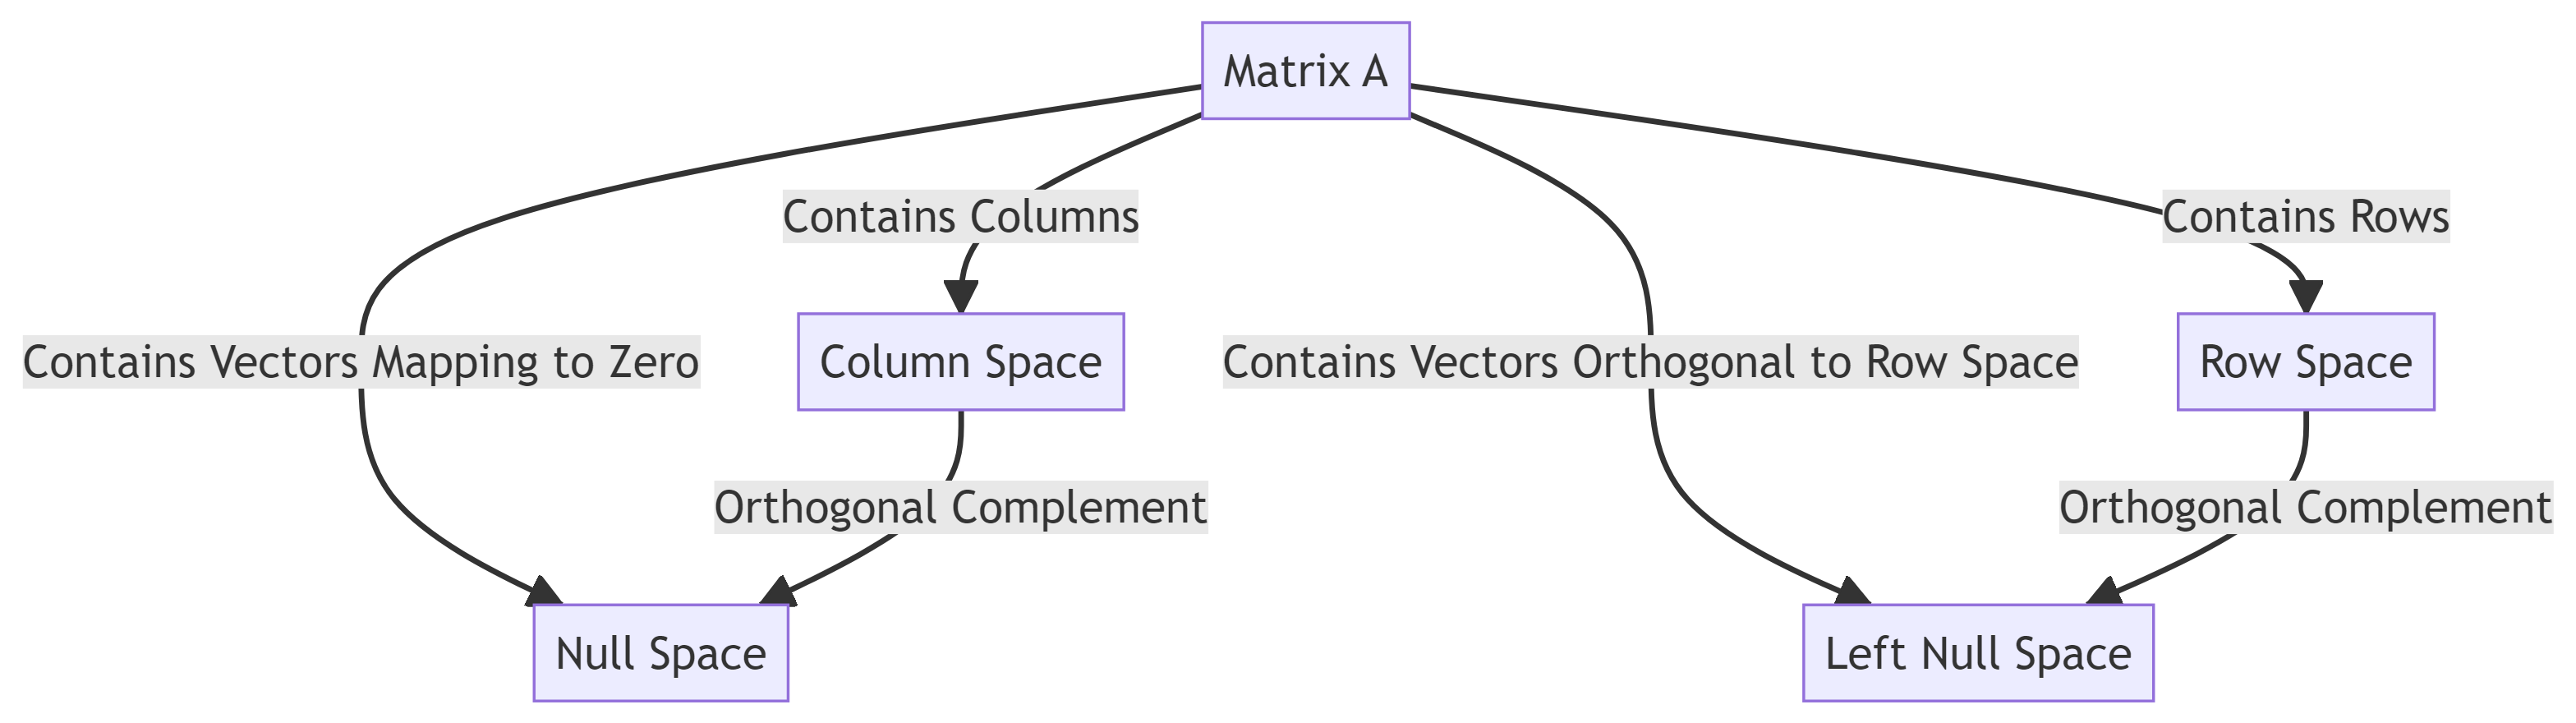
\includegraphics[width=9.49in,height=2.67in]{module_2_files/figure-latex/mermaid-figure-1.png}

This idea is depicted as a `Big picture of the four sub spaces of a
matrix' in the Strang's text book on Linear algebra for every one
(Strang 2020). This `Big Picture' is shown in Fig-~\ref{fig-big-pic}.

\begin{figure}

\centering{

\includegraphics[width=0.8\textwidth,height=\textheight]{index_files/mediabag/fbc5f91d82681dd7341d.png}

}

\caption{\label{fig-big-pic}The Big Pictue of Fundamental Subspaces}

\end{figure}%

A video session from Strang's session is here:

\url{https://youtu.be/rwLOfdfc4dw?si=DsJb8KJTF05hHc76}

\subsubsection{Practice Problems}\label{practice-problems-5}

\textbf{Problem 1:} Express the vector \((1,-2,5)\) as a linear
combination of the vectors \((1,1,1)\), \((1,2,3)\) and \((2,-1,1)\).

\textbf{Problem 2:} Show that the feature vector \((2,-5,3)\) is not
linearly associated with the features \((1,-3,2)\), \((2,-4,-1)\) and
\((1,-5,7)\).

\textbf{Problem 3:} Show that the feature vectors \((1,1,1)\),
\((1,2,3)\) and \((2,-1,1)\) are non-redundant.

\textbf{Problem 4:} Prove that the features \((1,-1,1)\), \((0,1,2)\)
and \((3,0,-1)\) form basis for the feature space.

\textbf{Problem 5:} Check whether the vectors \((1,2,1)\), \((2,1,4)\)
and \((4,5,6)\) form a basis for \(\mathbb{R}^3\).

\textbf{Problem 6:} Find the four fundamental subspaces of the feature
space created by \((1,2,1)\), \((2,1,4)\) and \((4,5,6)\).

\textbf{Problem 7:} Find the four fundamental subspaces and its
dimensions of the matrix
\(\begin{bmatrix}1&2&4\\2&1&5\\1&4&6\end{bmatrix}\).

\textbf{Problem 8:} Express
\(A=\begin{bmatrix}1&2&-1\\3&1&-1\\2&-1&0\end{bmatrix}\) as the
Kronecker product of the column space and the row space in the form
\(A=C\otimes R\).

\textbf{Problem 9:} Find the four fundamental subspaces of
\(A=\begin{bmatrix} 1&2&0&2&5\\-2&-5&1&-1&-8\\0&-3&3&4&1\\3&6&0&-7&2\end{bmatrix}\).

\textbf{Problem 10:} Find the four fundamental subspaces of
\(A=\begin{bmatrix}-1&2&-1&5&6\\4&-4&-4&-12&-8\\2&0&-6&-2&4\\-3&1&7&-2&12\end{bmatrix}\).

\textbf{Problem 11:} Express
\(A=\begin{bmatrix}2&3&-1&-1\\1&-1&-2&-4\\3&1&3&-2\\6&3&0&-7\end{bmatrix}\)
in \(A=C\otimes R\), where \(C\) is the column space and \(R\) is the
row space of \(A\).

\textbf{Problem 12:} Express
\(A=\begin{bmatrix}0&1&-3&-1\\1&0&1&1\\3&1&0&2\\1&1&-2&0\end{bmatrix}\)
in \(A=C\otimes R\), where \(C\) is the column space and \(R\) is the
row space of \(A\).

\textbf{Problem 13:} Show that the feature vectors \((2,3,0)\),
\((1,2,0)\) and \((8,13,0)\) are redundant and hence find the
relationship between them.

\textbf{Problem 14:} Show that the feature vectors \((1,2,1)\),
\((4,1,2)\), \((-3,8,1)\) and \((6,5,4)\) are redundant and hence find
the relationship between them.

\textbf{Problem 15:} Show that the feature vectors \((1,2,-1,0)\),
\((1,3,1,2)\), \((4,2,1,0)\) and \((6,1,0,1)\) are redundant and hence
find the relationship between them.

\begin{tcolorbox}[enhanced jigsaw, rightrule=.15mm, arc=.35mm, breakable, colback=white, toprule=.15mm, colframe=quarto-callout-important-color-frame, toptitle=1mm, opacityback=0, colbacktitle=quarto-callout-important-color!10!white, opacitybacktitle=0.6, title=\textcolor{quarto-callout-important-color}{\faExclamation}\hspace{0.5em}{Important}, bottomrule=.15mm, left=2mm, titlerule=0mm, coltitle=black, bottomtitle=1mm, leftrule=.75mm]

\textbf{Three Parts of the \emph{Fundamental theorem}} The fundamental
theorem of linear algebra relates all four of the fundamental subspaces
in a number of different ways. There are main parts to the theorem:

\textbf{Part 1:(Rank nullity theorem)} The column and row spaces of an
\(m\times n\) matrix \(A\) both have dimension \(r\), the rank of the
matrix. The nullspace has dimension \(n−r\), and the left nullspace has
dimension \(m−r\).

\textbf{Part 2:(Orthogonal subspaces)} The nullspace and row space are
orthogonal. The left nullspace and the column space are also orthogonal.

\textbf{Part 3:(Matrix decomposition)} The final part of the fundamental
theorem of linear algebra constructs an orthonormal basis, and
demonstrates a singular value decomposition: any matrix \(M\) can be
written in the form \(M=U\Sigma V^T\) , where \(U_{m\times m}\) and
\(V_{n\times n}\) are unitary matrices, \(\Sigma_{m\times n}\) matrix
with nonnegative values on the diagonal.

This part of the fundamental theorem allows one to immediately find a
basis of the subspace in question. This can be summarized in the
following table.

\begin{longtable}[]{@{}
  >{\centering\arraybackslash}p{(\columnwidth - 8\tabcolsep) * \real{0.2083}}
  >{\centering\arraybackslash}p{(\columnwidth - 8\tabcolsep) * \real{0.1250}}
  >{\centering\arraybackslash}p{(\columnwidth - 8\tabcolsep) * \real{0.2000}}
  >{\centering\arraybackslash}p{(\columnwidth - 8\tabcolsep) * \real{0.1000}}
  >{\centering\arraybackslash}p{(\columnwidth - 8\tabcolsep) * \real{0.3667}}@{}}
\toprule\noalign{}
\begin{minipage}[b]{\linewidth}\centering
Subspace
\end{minipage} & \begin{minipage}[b]{\linewidth}\centering
Subspace of
\end{minipage} & \begin{minipage}[b]{\linewidth}\centering
Symbol
\end{minipage} & \begin{minipage}[b]{\linewidth}\centering
Dimension
\end{minipage} & \begin{minipage}[b]{\linewidth}\centering
Basis
\end{minipage} \\
\midrule\noalign{}
\endhead
\bottomrule\noalign{}
\endlastfoot
Column space & \(\mathbb{R}^m\) & \(\operatorname{im}(A)\) & \(r\) &
First \(r\) columns of \(U\) \\
Nullspace (kernel) & \(\mathbb{R}^n\) & \(\ker(A)\) & \(n - r\) & Last
\(n - r\) columns of \(V\) \\
Row space & \(\mathbb{R}^n\) & \(\operatorname{im}(A^T)\) & \(r\) &
First \(r\) columns of \(V\) \\
Left nullspace (kernel) & \(\mathbb{R}^m\) & \(\ker(A^T)\) & \(m - r\) &
Last \(m - r\) columns of \(U\) \\
\end{longtable}

\end{tcolorbox}

\subsubsection{Computational methods to find all the four fundamental
subspaces of a
matrix}\label{computational-methods-to-find-all-the-four-fundamental-subspaces-of-a-matrix}

There are different approaches to find the four fundamental subspaces of
a matrix using \texttt{Python}. Simplest method is just convert our
mathematical procedure into \texttt{Python} functions and call them to
find respective spaces. This method is illustrated below.

\begin{Shaded}
\begin{Highlighting}[]
\CommentTok{\# importing numpy library for numerical computation}
\ImportTok{import}\NormalTok{ numpy }\ImportTok{as}\NormalTok{ np}
\CommentTok{\# define the function create the row{-}reduced Echelon form of given matrix}
\KeywordTok{def}\NormalTok{ row\_echelon\_form(A):}
    \CommentTok{"""Convert matrix A to its row echelon form."""}
\NormalTok{    A }\OperatorTok{=}\NormalTok{ A.astype(}\BuiltInTok{float}\NormalTok{)}
\NormalTok{    rows, cols }\OperatorTok{=}\NormalTok{ A.shape}
    \ControlFlowTok{for}\NormalTok{ i }\KeywordTok{in} \BuiltInTok{range}\NormalTok{(}\BuiltInTok{min}\NormalTok{(rows, cols)):}
        \CommentTok{\# Pivot: find the maximum element in the current column}
\NormalTok{        max\_row }\OperatorTok{=}\NormalTok{ np.argmax(np.}\BuiltInTok{abs}\NormalTok{(A[i:, i])) }\OperatorTok{+}\NormalTok{ i}
        \ControlFlowTok{if}\NormalTok{ A[max\_row, i] }\OperatorTok{==} \DecValTok{0}\NormalTok{:}
            \ControlFlowTok{continue}  \CommentTok{\# Skip if the column is zero}
        \CommentTok{\# Swap the current row with the max\_row}
\NormalTok{        A[[i, max\_row]] }\OperatorTok{=}\NormalTok{ A[[max\_row, i]]}
        \CommentTok{\# Eliminate entries below the pivot}
        \ControlFlowTok{for}\NormalTok{ j }\KeywordTok{in} \BuiltInTok{range}\NormalTok{(i }\OperatorTok{+} \DecValTok{1}\NormalTok{, rows):}
\NormalTok{            factor }\OperatorTok{=}\NormalTok{ A[j, i] }\OperatorTok{/}\NormalTok{ A[i, i]}
\NormalTok{            A[j, i:] }\OperatorTok{{-}=}\NormalTok{ factor }\OperatorTok{*}\NormalTok{ A[i, i:]}
    \ControlFlowTok{return}\NormalTok{ A}

\CommentTok{\# define function to generate null space from the row{-}reduced echelon form}
\KeywordTok{def}\NormalTok{ null\_space\_of\_matrix(A, rtol}\OperatorTok{=}\FloatTok{1e{-}5}\NormalTok{):}
    \CommentTok{"""Compute the null space of a matrix A using row reduction."""}
\NormalTok{    A\_reduced }\OperatorTok{=}\NormalTok{ row\_echelon\_form(A)}
\NormalTok{    rows, cols }\OperatorTok{=}\NormalTok{ A\_reduced.shape}
    \CommentTok{\# Identify pivot columns}
\NormalTok{    pivots }\OperatorTok{=}\NormalTok{ []}
    \ControlFlowTok{for}\NormalTok{ i }\KeywordTok{in} \BuiltInTok{range}\NormalTok{(rows):}
        \ControlFlowTok{for}\NormalTok{ j }\KeywordTok{in} \BuiltInTok{range}\NormalTok{(cols):}
            \ControlFlowTok{if}\NormalTok{ np.}\BuiltInTok{abs}\NormalTok{(A\_reduced[i, j]) }\OperatorTok{\textgreater{}}\NormalTok{ rtol:}
\NormalTok{                pivots.append(j)}
                \ControlFlowTok{break}
\NormalTok{    free\_vars }\OperatorTok{=} \BuiltInTok{set}\NormalTok{(}\BuiltInTok{range}\NormalTok{(cols)) }\OperatorTok{{-}} \BuiltInTok{set}\NormalTok{(pivots)}
    
\NormalTok{    null\_space }\OperatorTok{=}\NormalTok{ []}
    \ControlFlowTok{for}\NormalTok{ free\_var }\KeywordTok{in}\NormalTok{ free\_vars:}
\NormalTok{        null\_vector }\OperatorTok{=}\NormalTok{ np.zeros(cols)}
\NormalTok{        null\_vector[free\_var] }\OperatorTok{=} \DecValTok{1}
        \ControlFlowTok{for}\NormalTok{ pivot, row }\KeywordTok{in} \BuiltInTok{zip}\NormalTok{(pivots, A\_reduced[:}\BuiltInTok{len}\NormalTok{(pivots)]):}
\NormalTok{            null\_vector[pivot] }\OperatorTok{=} \OperatorTok{{-}}\NormalTok{row[free\_var]}
\NormalTok{        null\_space.append(null\_vector)}
    
    \ControlFlowTok{return}\NormalTok{ np.array(null\_space).T}

\CommentTok{\# define the function to generate the row{-}space of A}

\KeywordTok{def}\NormalTok{ row\_space\_of\_matrix(A):}
    \CommentTok{"""Compute the row space of a matrix A using row reduction."""}
\NormalTok{    A\_reduced }\OperatorTok{=}\NormalTok{ row\_echelon\_form(A)}
    \CommentTok{\# The non{-}zero rows of the reduced matrix form the row space}
\NormalTok{    non\_zero\_rows }\OperatorTok{=}\NormalTok{ A\_reduced[}\OperatorTok{\textasciitilde{}}\NormalTok{np.}\BuiltInTok{all}\NormalTok{(A\_reduced }\OperatorTok{==} \DecValTok{0}\NormalTok{, axis}\OperatorTok{=}\DecValTok{1}\NormalTok{)]}
    \ControlFlowTok{return}\NormalTok{ non\_zero\_rows}

\CommentTok{\# define the function to generate the column space of A}

\KeywordTok{def}\NormalTok{ column\_space\_of\_matrix(A):}
    \CommentTok{"""Compute the column space of a matrix A using row reduction."""}
\NormalTok{    A\_reduced }\OperatorTok{=}\NormalTok{ row\_echelon\_form(A)}
\NormalTok{    rows, cols }\OperatorTok{=}\NormalTok{ A\_reduced.shape}
    \CommentTok{\# Identify pivot columns}
\NormalTok{    pivots }\OperatorTok{=}\NormalTok{ []}
    \ControlFlowTok{for}\NormalTok{ i }\KeywordTok{in} \BuiltInTok{range}\NormalTok{(rows):}
        \ControlFlowTok{for}\NormalTok{ j }\KeywordTok{in} \BuiltInTok{range}\NormalTok{(cols):}
            \ControlFlowTok{if}\NormalTok{ np.}\BuiltInTok{abs}\NormalTok{(A\_reduced[i, j]) }\OperatorTok{\textgreater{}} \FloatTok{1e{-}5}\NormalTok{:}
\NormalTok{                pivots.append(j)}
                \ControlFlowTok{break}
\NormalTok{    column\_space }\OperatorTok{=}\NormalTok{ A[:, pivots]}
    \ControlFlowTok{return}\NormalTok{ column\_space}
\end{Highlighting}
\end{Shaded}

\subsubsection{Examples:}\label{examples}

\begin{enumerate}
\def\labelenumi{\arabic{enumi}.}
\tightlist
\item
  Find all the fundamental subspaces of
  \(A=\begin{pmatrix}1&2&3\\ 4&5&6\\7&8&9\end{pmatrix}\).
\end{enumerate}

\begin{Shaded}
\begin{Highlighting}[]
\NormalTok{A }\OperatorTok{=}\NormalTok{ np.array([[}\DecValTok{1}\NormalTok{, }\DecValTok{2}\NormalTok{, }\DecValTok{3}\NormalTok{],}
\NormalTok{              [}\DecValTok{4}\NormalTok{, }\DecValTok{5}\NormalTok{, }\DecValTok{6}\NormalTok{],}
\NormalTok{              [}\DecValTok{7}\NormalTok{, }\DecValTok{8}\NormalTok{, }\DecValTok{9}\NormalTok{]])}

\BuiltInTok{print}\NormalTok{(}\StringTok{"Matrix A:"}\NormalTok{)}
\BuiltInTok{print}\NormalTok{(A)}

\CommentTok{\# Null Space}
\NormalTok{null\_space\_A }\OperatorTok{=}\NormalTok{ null\_space\_of\_matrix(A)}
\BuiltInTok{print}\NormalTok{(}\StringTok{"}\CharTok{\textbackslash{}n}\StringTok{Null Space of A:"}\NormalTok{)}
\BuiltInTok{print}\NormalTok{(null\_space\_A)}

\CommentTok{\# Row Space}
\NormalTok{row\_space\_A }\OperatorTok{=}\NormalTok{ row\_space\_of\_matrix(A)}
\BuiltInTok{print}\NormalTok{(}\StringTok{"}\CharTok{\textbackslash{}n}\StringTok{Row Space of A:"}\NormalTok{)}
\BuiltInTok{print}\NormalTok{(row\_space\_A)}

\CommentTok{\# Column Space}
\NormalTok{column\_space\_A }\OperatorTok{=}\NormalTok{ column\_space\_of\_matrix(A)}
\BuiltInTok{print}\NormalTok{(}\StringTok{"}\CharTok{\textbackslash{}n}\StringTok{Column Space of A:"}\NormalTok{)}
\BuiltInTok{print}\NormalTok{(column\_space\_A)}
\end{Highlighting}
\end{Shaded}

\begin{verbatim}
Matrix A:
[[1 2 3]
 [4 5 6]
 [7 8 9]]

Null Space of A:
[[-9.        ]
 [-1.71428571]
 [ 1.        ]]

Row Space of A:
[[7.00000000e+00 8.00000000e+00 9.00000000e+00]
 [0.00000000e+00 8.57142857e-01 1.71428571e+00]
 [0.00000000e+00 5.55111512e-17 1.11022302e-16]]

Column Space of A:
[[1 2]
 [4 5]
 [7 8]]
\end{verbatim}

\subsubsection{Rank and Solution of System of Linear
Equations}\label{rank-and-solution-of-system-of-linear-equations}

In linear algebra, the rank of a matrix is a crucial concept for
understanding the structure of a system of linear equations. It provides
insight into the solutions of these systems, helping us determine the
number of independent equations and the nature of the solution space.

\begin{definition}[Rank and System
Consistency]\protect\hypertarget{def-soln}{}\label{def-soln}

The rank of a matrix \(A\) is defined as the maximum number of linearly
independent rows or columns. When solving a system of linear equations
represented by \(A\mathbf{x} = \mathbf{b}\), where \(A\) is an
\(m \times n\) matrix and \(\mathbf{b}\) is a vector, the rank of \(A\)
plays a crucial role in determining the solution's existence and
uniqueness.

\textbf{Consistency of the System}

\begin{enumerate}
\def\labelenumi{\arabic{enumi}.}
\tightlist
\item
  \textbf{Consistent System:} A system of linear equations is consistent
  if there exists at least one solution. This occurs if the rank of the
  coefficient matrix \(A\) is equal to the rank of the augmented matrix
  \([A|\mathbf{b}]\). Mathematically, this can be expressed as:
  \[\text{rank}(A) = \text{rank}([A|\mathbf{b}])\] If this condition is
  met, the system has solutions. The solutions can be:

  \begin{itemize}
  \tightlist
  \item
    \textbf{Unique} if the rank equals the number of variables.
  \item
    \textbf{Infinitely many} if the rank is less than the number of
    variables.
  \end{itemize}
\item
  \textbf{Inconsistent System:} A system is inconsistent if there are no
  solutions. This occurs when:
  \[\text{rank}(A) \ne \text{rank}([A|\mathbf{b}])\] In this case, the
  equations represent parallel or conflicting constraints that cannot be
  satisfied simultaneously.
\end{enumerate}

\end{definition}

\begin{tcolorbox}[enhanced jigsaw, rightrule=.15mm, arc=.35mm, breakable, colback=white, toprule=.15mm, colframe=quarto-callout-note-color-frame, toptitle=1mm, opacityback=0, colbacktitle=quarto-callout-note-color!10!white, opacitybacktitle=0.6, title=\textcolor{quarto-callout-note-color}{\faInfo}\hspace{0.5em}{Use of Null space in creation of general solution from particular
solution}, bottomrule=.15mm, left=2mm, titlerule=0mm, coltitle=black, bottomtitle=1mm, leftrule=.75mm]

If the system \(AX=b\) has many solutions, then the general solution of
the system can be found using a particular solution and the elements in
the null space of the coefficient matrix \(A\) as

\[X=x_p+tX_N\]

where \(X\) is the general solution and \(t\) is a free variable
(parameter) and \(X_N\in N(A)\).

\end{tcolorbox}

\subsubsection{Computational method to solve system of linear
equations.}\label{computational-method-to-solve-system-of-linear-equations.}

If for a system \(AX=b\), \(det(A)\neq 0\), then the system has a unique
solution and can be found by \texttt{solve()} function from
\texttt{NumPy}. If the system is consistant and many solutions, then
computationally we will generate the general solution using the
\(N(A)\). A detailed \texttt{Python} code is given below.

\begin{Shaded}
\begin{Highlighting}[]
\ImportTok{import}\NormalTok{ numpy }\ImportTok{as}\NormalTok{ np}

\KeywordTok{def}\NormalTok{ check\_consistency(A, b):}
    \CommentTok{"""}
\CommentTok{    Check the consistency of a linear system Ax = b and return the solution if consistent.}
\CommentTok{    }
\CommentTok{    Parameters:}
\CommentTok{    A (numpy.ndarray): Coefficient matrix.}
\CommentTok{    b (numpy.ndarray): Right{-}hand side vector.}
\CommentTok{    }
\CommentTok{    Returns:}
\CommentTok{    tuple: A tuple with consistency status, particular solution (if consistent), and null space (if infinite solutions).}
\CommentTok{    """}
\NormalTok{    A }\OperatorTok{=}\NormalTok{ np.array(A)}
\NormalTok{    b }\OperatorTok{=}\NormalTok{ np.array(b)}
    
    \CommentTok{\# Augment the matrix A with vector b}
\NormalTok{    augmented\_matrix }\OperatorTok{=}\NormalTok{ np.column\_stack((A, b))}
    
    \CommentTok{\# Compute ranks}
\NormalTok{    rank\_A }\OperatorTok{=}\NormalTok{ np.linalg.matrix\_rank(A)}
\NormalTok{    rank\_augmented }\OperatorTok{=}\NormalTok{ np.linalg.matrix\_rank(augmented\_matrix)}
    
    \CommentTok{\# Check for consistency}
    \ControlFlowTok{if}\NormalTok{ rank\_A }\OperatorTok{==}\NormalTok{ rank\_augmented:}
        \ControlFlowTok{if}\NormalTok{ rank\_A }\OperatorTok{==}\NormalTok{ A.shape[}\DecValTok{1}\NormalTok{]:}
            \CommentTok{\# Unique solution}
\NormalTok{            solution }\OperatorTok{=}\NormalTok{ np.linalg.solve(A, b)}
            \ControlFlowTok{return} \StringTok{"Consistent and has a unique solution"}\NormalTok{, solution, }\VariableTok{None}
        \ControlFlowTok{else}\NormalTok{:}
            \CommentTok{\# Infinitely many solutions}
\NormalTok{            particular\_solution }\OperatorTok{=}\NormalTok{ np.linalg.lstsq(A, b, rcond}\OperatorTok{=}\VariableTok{None}\NormalTok{)[}\DecValTok{0}\NormalTok{]}
\NormalTok{            null\_space }\OperatorTok{=}\NormalTok{ null\_space\_of\_matrix(A)}
            \ControlFlowTok{return} \StringTok{"Consistent but has infinitely many solutions"}\NormalTok{, particular\_solution, null\_space}
    \ControlFlowTok{else}\NormalTok{:}
        \ControlFlowTok{return} \StringTok{"Inconsistent system (no solution)"}\NormalTok{, }\VariableTok{None}\NormalTok{, }\VariableTok{None}

\KeywordTok{def}\NormalTok{ null\_space\_of\_matrix(A):}
    \CommentTok{"""}
\CommentTok{    Compute the null space of matrix A, which gives the set of solutions to Ax = 0.}
\CommentTok{    }
\CommentTok{    Parameters:}
\CommentTok{    A (numpy.ndarray): Coefficient matrix.}
\CommentTok{    }
\CommentTok{    Returns:}
\CommentTok{    numpy.ndarray: Basis for the null space of A.}
\CommentTok{    """}
\NormalTok{    u, s, vh }\OperatorTok{=}\NormalTok{ np.linalg.svd(A)}
\NormalTok{    null\_mask }\OperatorTok{=}\NormalTok{ (s }\OperatorTok{\textless{}=} \FloatTok{1e{-}10}\NormalTok{)  }\CommentTok{\# Singular values near zero}
\NormalTok{    null\_space }\OperatorTok{=}\NormalTok{ np.compress(null\_mask, vh, axis}\OperatorTok{=}\DecValTok{0}\NormalTok{)}
    \ControlFlowTok{return}\NormalTok{ null\_space.T}
\end{Highlighting}
\end{Shaded}

\begin{quote}
\emph{Example 1:} Solve
\begin{align*}2x-y+z&=1\\ x+2y&=3\\ 3x+2y+z&=4\end{align*}
\end{quote}

\begin{Shaded}
\begin{Highlighting}[]
\CommentTok{\# Example usage 1: System with a unique solution}
\NormalTok{A1 }\OperatorTok{=}\NormalTok{ np.array([[}\DecValTok{2}\NormalTok{, }\OperatorTok{{-}}\DecValTok{1}\NormalTok{, }\DecValTok{1}\NormalTok{], [}\DecValTok{1}\NormalTok{, }\DecValTok{0}\NormalTok{, }\DecValTok{2}\NormalTok{], [}\DecValTok{3}\NormalTok{, }\DecValTok{2}\NormalTok{, }\DecValTok{1}\NormalTok{]])}
\NormalTok{b1 }\OperatorTok{=}\NormalTok{ np.array([}\DecValTok{1}\NormalTok{, }\DecValTok{3}\NormalTok{, }\DecValTok{4}\NormalTok{])}

\NormalTok{status1, solution1, null\_space1 }\OperatorTok{=}\NormalTok{ check\_consistency(A1, b1)}
\BuiltInTok{print}\NormalTok{(}\StringTok{"Example 1 {-} Status:"}\NormalTok{, status1)}

\ControlFlowTok{if}\NormalTok{ solution1 }\KeywordTok{is} \KeywordTok{not} \VariableTok{None}\NormalTok{:}
    \BuiltInTok{print}\NormalTok{(}\StringTok{"Solution:"}\NormalTok{, solution1)}
\ControlFlowTok{if}\NormalTok{ null\_space1 }\KeywordTok{is} \KeywordTok{not} \VariableTok{None}\NormalTok{:}
    \BuiltInTok{print}\NormalTok{(}\StringTok{"Null Space:"}\NormalTok{, null\_space1)}
\end{Highlighting}
\end{Shaded}

\begin{verbatim}
Example 1 - Status: Consistent and has a unique solution
Solution: [0.27272727 0.90909091 1.36363636]
\end{verbatim}

\begin{quote}
\emph{Example 2:} Solve the system of equations,
\textbackslash begin\{align*\}x+2y+z\&=3\textbackslash{}
2x+4y+2z\&=6\textbackslash{} x+y+z\&=2\textbackslash end\{align\}
\end{quote}

\begin{Shaded}
\begin{Highlighting}[]
\CommentTok{\# Example usage 2: System with infinitely many solutions}
\NormalTok{A2 }\OperatorTok{=}\NormalTok{ np.array([[}\DecValTok{1}\NormalTok{, }\DecValTok{2}\NormalTok{, }\DecValTok{1}\NormalTok{], [}\DecValTok{2}\NormalTok{, }\DecValTok{4}\NormalTok{, }\DecValTok{2}\NormalTok{], [}\DecValTok{1}\NormalTok{, }\DecValTok{1}\NormalTok{, }\DecValTok{1}\NormalTok{]])}
\NormalTok{b2 }\OperatorTok{=}\NormalTok{ np.array([}\DecValTok{3}\NormalTok{, }\DecValTok{6}\NormalTok{, }\DecValTok{2}\NormalTok{])}

\NormalTok{status2, solution2, null\_space2 }\OperatorTok{=}\NormalTok{ check\_consistency(A2, b2)}
\BuiltInTok{print}\NormalTok{(}\StringTok{"}\CharTok{\textbackslash{}n}\StringTok{Example 2 {-} Status:"}\NormalTok{, status2)}

\ControlFlowTok{if}\NormalTok{ solution2 }\KeywordTok{is} \KeywordTok{not} \VariableTok{None}\NormalTok{:}
    \BuiltInTok{print}\NormalTok{(}\StringTok{"Particular Solution:"}\NormalTok{, solution2)}
\ControlFlowTok{if}\NormalTok{ null\_space2 }\KeywordTok{is} \KeywordTok{not} \VariableTok{None}\NormalTok{:}
    \BuiltInTok{print}\NormalTok{(}\StringTok{"Null Space (Basis for infinite solutions):"}\NormalTok{, null\_space2)}
\end{Highlighting}
\end{Shaded}

\begin{verbatim}

Example 2 - Status: Consistent but has infinitely many solutions
Particular Solution: [0.5 1.  0.5]
Null Space (Basis for infinite solutions): [[ 7.07106781e-01]
 [ 1.11022302e-16]
 [-7.07106781e-01]]
\end{verbatim}

\begin{tcolorbox}[enhanced jigsaw, rightrule=.15mm, arc=.35mm, breakable, colback=white, toprule=.15mm, colframe=quarto-callout-note-color-frame, toptitle=1mm, opacityback=0, colbacktitle=quarto-callout-note-color!10!white, opacitybacktitle=0.6, title=\textcolor{quarto-callout-note-color}{\faInfo}\hspace{0.5em}{Connection between fundamental subspaces and Singular Value
Decomposition}, bottomrule=.15mm, left=2mm, titlerule=0mm, coltitle=black, bottomtitle=1mm, leftrule=.75mm]

Every non zero matrix can be expressed as a decomposition known as the
SVD as follows:

\begin{align}
  \mathbf{A} &=
  \mathbf{U} \, \Sigma \, \mathbf{V}^{*} \\
%
 &=
% U 
  \left[ \begin{array}{cc}
     \color{blue}{\mathbf{U}_{\mathcal{R}}} & \color{red}{\mathbf{U}_{\mathcal{N}}}
  \end{array} \right]  
% Sigma
  \left[ \begin{array}{cccc|cc}
     \sigma_{1} & 0 & \dots &  &   & \dots &  0 \\
     0 & \sigma_{2}  \\
     \vdots && \ddots \\
       & & & \sigma_{\rho} \\\hline
       & & & & 0 & \\
     \vdots &&&&&\ddots \\
     0 & & &   &   &  & 0 \\
  \end{array} \right]
% V 
  \left[ \begin{array}{c}
     \color{blue}{\mathbf{V}_{\mathcal{R}}}^{*} \\ 
     \color{red}{\mathbf{V}_{\mathcal{N}}}^{*}
  \end{array} \right]  \\
%
  & =
% U
   \left[ \begin{array}{cccccccc}
    \color{blue}{u_{1}} & \dots & \color{blue}{u_{\rho}} & \color{red}{u_{\rho+1}} & \dots & \color{red}{u_{m}}
  \end{array} \right]
% Sigma
  \left[ \begin{array}{cc}
     \mathbf{S}_{\rho\times \rho} & \mathbf{0} \\
     \mathbf{0} & \mathbf{0} 
  \end{array} \right]
% V
   \left[ \begin{array}{c}
    \color{blue}{v_{1}^{*}} \\ 
    \vdots \\
    \color{blue}{v_{\rho}^{*}} \\
    \color{red}{v_{\rho+1}^{*}} \\
    \vdots \\ 
    \color{red}{v_{n}^{*}}
  \end{array} \right]
%
\end{align}

The column vectors form spans for the subspaces:

\begin{align} 
% R A
\color{blue}{\mathcal{R} \left( \mathbf{A} \right)} &=
\text{span} \left\{
 \color{blue}{u_{1}}, \dots , \color{blue}{u_{\rho}}
\right\} \\
% R A*
\color{blue}{\mathcal{R} \left( \mathbf{A}^{*} \right)} &=
\text{span} \left\{
 \color{blue}{v_{1}}, \dots , \color{blue}{v_{\rho}}
\right\} \\
% N A*
\color{red}{\mathcal{N} \left( \mathbf{A}^{*} \right)} &=
\text{span} \left\{
\color{red}{u_{\rho+1}}, \dots , \color{red}{u_{m}}
\right\} \\
% N A
\color{red}{\mathcal{N} \left( \mathbf{A} \right)} &=
\text{span} \left\{
\color{red}{v_{\rho+1}}, \dots , \color{red}{v_{n}}
\right\} \\
%
\end{align}

The conclusion is that the full SVD provides an orthonormal span for not
only the two null spaces, but also both range spaces.

\end{tcolorbox}

\bookmarksetup{startatroot}

\chapter*{References}\label{references}
\addcontentsline{toc}{chapter}{References}

\markboth{References}{References}

\phantomsection\label{refs}
\begin{CSLReferences}{1}{0}
\bibitem[\citeproctext]{ref-knuth84}
Knuth, Donald E. 1984. {``Literate Programming.''} \emph{Comput. J.} 27
(2): 97--111. \url{https://doi.org/10.1093/comjnl/27.2.97}.

\bibitem[\citeproctext]{ref-strang2020linear}
Strang, Gilbert. 2020. \emph{Linear Algebra for Everyone}. SIAM.

\bibitem[\citeproctext]{ref-strang2022introduction}
---------. 2022. \emph{Introduction to Linear Algebra}. SIAM.

\end{CSLReferences}




\end{document}
